\documentclass[b5j,11pt]{jsbook}
%\documentclass[b5j,10pt,tombo]{jsbook}

%\usepackage[dviout]{graphicx}

\usepackage[dvipdfmx]{graphicx}

% フォントメトリック指定
\usepackage{minijs}
\usepackage{otf}

\usepackage{makeidx}
\usepackage{booktabs}
\usepackage{tabularx}
\usepackage{wrapfig}
\usepackage{moreverb}
\usepackage{amsmath}
\usepackage{amssymb}
\usepackage{fancybox}
\usepackage{ascmac}
\usepackage{listings,jlisting}
\usepackage[avantgarde]{quotchap}

%\renewcommand{\baselinestretch}{0.5}
%\renewcommand{\baselinestretch}{0.6}
\renewcommand{\baselinestretch}{0.7}

\begin{document}
\title{同人版TCP/IP入門 第四版 IPv6対応版}
\author{AliceSystem ありす ゆう インフラエンジニアの毒舌な妹 共著}
\date{第四版発行 2016年8月14日}
\maketitle
\frontmatter
\section*{謝辞}
\begin{center}
この本を読んでくださる方に \\
気力をくれる友人に \\
大切な人に \\
感謝と本書をささげます
\end{center}

\section*{初版前書き}
ネットワーク対応製品を開発していても、プログラマはTCP/IPやイーサネットのことをあまりよく理解していない。そんな現状があります。

そうでなくても、ゲーム用のNICなんてオカルトな製品が出てくる世の中。同じお金で、Intelか3comのNICを買っておいたほうが幸せになれる、ということを理解するためには、ネットワーク技術の知識が欠かせません。

本書は、そのための解説書として作成しました。TCP/IP理解の一助となれば幸いです。


\section*{改訂版前書き}
コミックマーケット78で本書の初版を出しました。90ページ近いとはいえ、コピー本としては500円という無茶な値段\footnote{キンコーズでのコピー代とホチキスの3号針の代金を回収させていただいた程度です。}にもかかわらず、もっていった20部が午前中に完売という、ありがたくも自分にとっての誤算となる事態となりました。

その後、見本誌を自分でチェックすると細かい間違いも誤字脱字もいっぱいみつけて…テクノポリスかゲーメストか、という有様に、単なる再版でなく、全面的なリライトをしたのが、本書です。

IPv4という、当面使い続けることになるとしても、いつかIPv6に取って代わられてほしいテクノロジーをもとに解説していくのもどうかと思いました。せっかく同人誌なのだから、IPv6でTCP/IPの教科書というのも…さすがに無理です。

本というのは、著者が理解していない項目を文章にしても、読者には理解してもらえません。本書は、著者の判る範囲でTCP/IPについてまとめています。

\section*{第三版前書き}
コミックマーケット79ではじめてオンデマンド本にした改訂版も、コミックマーケット80にて完売させていただきました。
そうなるとまた直したくなるもので…それなんてオライリー商法、という感じではありますが、現在の知識をもとに、記事の追加修正を行いました。こっそり間違いも直しています。

一番大きな変更は、章立てを見直したことでしょう。本書の二章と三章、七章から九章までは、前の版ではひとつの章でした。分割することで、異なることの詰め込み感があったことを少しなりとも解消できたかなと思います。、

またIPv4か、という感想を頂く覚悟はしていますが、やはりIPv4は現在のインターネット技術の基本です。完売した\footnote{本書改訂版でなくもちろんIPv4アドレスのことです。}とはいえまだまだ現場では現役でしょう。\footnote{IPv6環境での疑似ヘッダってどうなるんだろう…}
IPv6を理解する基礎体力作りに、是非本書をご活用ください。

インターネットで使用されている技術の基礎を、少しなりとも理解していただく助けになれば幸いです。少なくとも、参考文献に期した書籍をひもとくきっかけになれればと思います。

\section*{第四版前書き}
当サークルで毎回サークルカットに書いているくせに、出そうで出ない本であった本書ですが、5年のブランクを経て、ようやく、更なる改訂版が出せました。今回は、念願のIPv6対応です。

今回は、章立てを大胆に入れ替えてみました。これまではネットワークアクセス層から上のレイヤに向かっての説明を行っていたのですが、アプリケーション層からトランスポート層への説明、ネットワークアクセス層の説明を経て、、いわば上のレイヤと下のレイヤの知識を付けてから、インターネットプロトコル層について学ぶ形にしてみました。

また、本書ではUDPが一番最後の章という変則的な後世になっています。これは、パケットそのものであるUDPは、いわばパンツをはいたIPである、という理屈のもと、UDPの理解にはIPの理解が必要なのではないか、そう考えたからです。

また、すっかり当サークルの顔になっている、インフラエンジニアの毒舌な妹に、章の序文と、いもうとコラムというコーナーを担当して貰いました。本書では、インフラエンジニアの毒舌名妹は、TCP/IPについて、いろいろな関連知識の説明を担当しています。


特にIPv6についてはまだまだ書き足りないところもありますが、IPv4を使うTCP/IPと、IPv6を使うTCP/IP、その同じところ、違うところの知見を得ていただければ、筆者としては幸いです。

\section*{第六版前書き}
世の中は、スマホアプリを始めとして、ネットワーク対応のアプリケーションがあふれています。
その状況で、TCP/IPについて、基本的な部分を纏めた本というのはあまりありません。流行りの言語やフレームワークと比べると、新規性がないせいか数量的な見劣りがします。

そんな中、本書は、TCP/IPのことをわからないと言えないままネットワークアプリケーションを開発しているエンジニアが、TCP/IPの基本を理解するための本として、加筆訂正を行いました。

特に、IPv6については、IPv4ベースのTCP/IPの理解を前提としているネットワークエンジニア向けの本が多いため、TCP/IPの一部として初学者が学ぶためのテキストとは多くありません。
そこで、今回の版では、第四版からIPv6に関する記述を増やし、TCP/IPのなかにあるiPv6を意識して貰えるようにしました。
また、第四版は、TCP/IPのレイヤーの順番に拘らない解説を試みたのですが、立ち入った説明をするための前提条件の説明のため、代三版以前の構成に戻しています。

あわせて、プロキシ、`NATN、NAPTに関する記事を追加しました。これらは現在では家庭のネットワークにも存在するものです。ネットワークアプリケーションを開発するときに意識しておくべきものであるため、コミックマーケット92で出した同人誌から再録し、本書の内容に合わせての加筆訂正を行っています。

皆様が、TCP/IPについて知る一助となれば、著者としてこれに勝る喜びはありません。

\section*{想定する読者}
IT関連でプログラマなどをしていて、普段はネットワークのことを気にしない人に、TCP/IPと、その物理インフラの代表であるイーサネットについて、について最低限理解してもらう、というコンセプトで書いています。想定する読者は、TCP/IPについて、正面から勉強したことはないけれど、何となくネットワークアプリケーションのプログラムを書いている、そんなエンジニアです。

そのため、インフラエンジニアの視点で見ると若干物足りない部分があるかと思います。この点は今後の本で埋めていきたいところです。


\section*{本書の内容}
本書では、TCP/IPについて、IPv4とIPv6を一度に学習するというコンセプトで、TCP/IPの解説を行っています。

\paragraph{第一章}
TCP/IPというプロトコルの概論と、おおまかな全体像と、プロトコルスタックの概念についてについて説明します。TCP/IPは、複数のプロトコルが、役割を分担しながら他のプロトコルにサービスしたり、他のプロトコルからサービスを受けたりして通信をすることについての説明です。

\paragraph{第二章}
ネットワークの物理媒体とその上での通信である、ネットワークアクセス層の概論と、一番簡単なネットワークである、エンドとエンドにホストがある、一対一通信のネットワークについての説明です。

\paragraph{第三章}
ネットワークアクセス層で、一つの伝送媒体を複数のホストが共有するネットワークについて、説明を行います。その代表として、イーサネットの説明を行います。

\paragraph{第四章}
トランスポート層についての概論的な説明です。トランスポート層における確実な通信とは何か、確実な通信が要らない場合、どのように通信を行うか、上位のアプリケーションとの対応付けはどのようにおこなうか、UDPやTCPの理解のために必要な知識についての説明をします。

\paragraph{第五章}
トランスポート層のプロトコルのひとつであるUDPについて説明します。UDPは、インターネットプロトコル層の機能に、ポートによる通信多重化とエラー検出を付加した、比較的簡単な簡単なトランスポート層となります。

\paragraph{第六章}
トランスポート層のプロトコルのひとつ、ストリーム通信を提供するTCPについて説明します。TCPは下位のプロトコルが何であるかにもかかわらず、確実な通信を提供するプロトコルです。

\paragraph{第七章}
アプリケーション層についての説明となります。電子メールのSMTPなど、アプリケーション層のプロトコルについて説明をします。また、アプリケーションでIPv6対応ついても説明をします。

\paragraph{第八章}
アプリケーション層での通信を中継するプロキシについて説明します。
プロキシという、ルータと別の概念で中継をするというのはどういうことかについての解説です。

\paragraph{第九章}
プロキシという概念でインターネットプロトコル層の中継をおこなうNATについての説明をします。TCP/IPの知識を踏まえて、中継のためにヘッダ情報を書き換えることの副作用について乃解説を行います。



\paragraph{第十章}
トランスポート層の中継を行うプロキシであるNAPTについて説明します。IPv4ベースのネットワークで、少ないグローバルアドレスを共有するための技術であり、現在のインターネットを理解するためには必要な概念です。


\section*{免責事項}
本書に書いてあることは、筆者知識のレベルでまとめたものです。ですが、内容が正しいとは言い切れません。初版でも改訂版でも相当やらかしています。また、学校のレポート、業務などのコードを書く際に、本書の内容を信じて書いて損害が生じても、筆者にその責任はありません。

くれぐれも、自己責任と十分な検証の上、ご利用ください。

\section*{表紙イラスト}
ゆうちゃん (コース英知)
\tableofcontents
\listoffigures
\mainmatter
\chapter{TCP/IPの概論}

TCP/IPはいまいちわかりにくいですよね。

インターネットを経由しての通信は、TCP/IPで行われているのは知っているでしょう。でも、アプリケーションから見たとき、TCPとかIPとかがどんな役割をしているから、離れたサーバとクライアントが通信できるのか。また、LANとインターネットとはどんな風に繋がっているのか。そんな部分がよくわからない。

まずは、TCP/IPというもののイメージを掴んでみることにしましょう。

この章では、通信を行う両社を、慣例に従ってAliceとBobという名前で表記します。

\section{鳥類キャリアによるIP伝送}

伝書鳩でインターネット通信ができる。そのための規格があることをご存知だろうか。

インターネットにおける規格を提案するRFC\footnote{Request for Comment}の1149番で、鳥類キャリアによるIP伝送(IPoAC IP over Avian Carrier)という規格が提案されている。\footnote{https://tools.ietf.org/html/rfc1149}

IPoACについて簡単に説明すれば、紙に通信したいデータを書いて、伝書鳩\footnote{規格ではavian carrierであり、伝書『鳩』と明記はされていない}にくくりつけて飛ばす、そうやってインターネットの通信を行う手順の提案である。
このように、IPoACは、鳩に持たせるための紙に書いたデータを作成する規約、鳩の挙動などについて言及し、伝書鳩をインターネットの通信に使用できるようにした規格の提案として提出されたものだ。

種を明かせば、IPoACは1990年4月1日に発行された提案であり、ジョークRFCと呼ばれるもののひとつである。RFCでは、毎年4月1日非は、このようなジョークRFCを発行する習慣がある。

IPoACはジョークRFCではあったが、実証実験が行われている。その実証実験では、鳩が宛先に辿り着かなかったことによって生ずるデータの損失が多く、鳩なので伝送遅延も大きい。つまり、通信のやり直しや通信そのものにかかる時間が大きいという、ある意味当然の結論が出た。
だが、IPoACは、これらの問題を許容すれば、伝書鳩でインターネットの通信を行うことが可能であることも、その実証実験でしめした。



\section*{}
\begin{itembox}[l]{いもうとコラム 惑星間インターネット}
RFC1149はいわゆるジョークRFCでしたが、、インターネット通信において、送ったデータのロストや応答時間(レイテンシ)が大きくなる環境があります。
それは、宇宙です。さよならジュピターでも、カイパーベルト領域ま行った探査船のコンピュータであるナヴァホと、月に設置されたコンピュータのティム・ラビットがレイテンシを越えて会話するシーンがありました。

このような環境のインターネット通信は、惑星間インターネット(Interplanetary Internet)として研究開発が行われています。
\end{itembox}


\section{伝書鳩でインターネットの通信をするための仕組み}
鳩は遅い。そして、送り出した鳩が、目的とする通信相手にたどり着くわけでもない。また、順番通りに届くわけでもない。だが、鳩を伝送媒体に用いて、でインターネットで行われている通信が成立する。

そのような条件で通信ができるようにするには、どうすればよいのだろうか。それは、伝送遅延を許容し、鳩は確率的にしか相手のところにたどり着かず、送り出した順番と到着した順番が一致しないことを前提に通信の仕組みを作る。つまり、鳩に完璧さを求めず、それをサポートする仕組みをつくれがよい。

伝書鳩の役割とは、通信を行う双方の間で、情報を物理的な空間を越えて運ぶことである。
鳩なので、途中で餌になる虫を見つけたり、発情期で交尾相手を見つけたり、鷹に追いかけられて逃げたりするかもしれない。これらの可能性は、IPoACでも検討されている。
鳩は、通信の焚いての所に到着する時間がわからない。それどころか、相手のところに到着しないこともある。送り出した順番に鳩が到着することもないだろう。

まず、鳩なのだから、必ずしも通信の相手側に到着するわけではない。これを前提条件として、伝書鳩で通信をするための仕組みを考えて聞くことにしよう。


\subsection{鳩を使って確実な通信をする方法}

現在のインターネットは、確実な通信を行っている。だが、IPoACを使ってインターネットの通信を行うのうなら、データを運ぶ手段が鳩であるという前提で、確実な通信をおこなう手段をかなが得なければならない。
それは、相手にデータが届いたことがわかるまで、同じデータを送り直し続ける、ということである。この過程をくりかえしていけば、確率的にいつか通信が成功するだろう。


最初に、AliceとBobで、鳩が行き来できる状況なのかを確認する。その確認が取れないと、いくら鳩を飛ばしても通信が成立しない可能性があるということだ。

次に、鳩が届けたデータを受け取った側は、Aliceに向けて飛ぶ鳩を使って、データを受け取ったという返事をすることにする。
このとき、データを運ぶ手段は鳩しかない。電話など、鳩以外の手段で通信を届けることはできない。

三つ目、データを送信した側は、一定時間待って、データを受け取ったことを知らせる鳩が通信お相手から来なければ、送り出した鳩が到着しなかったとみなして、もう一度鳩を送り出す。
これは、相手がデータを受け取ったことが確認できるまで3は、そのデータは届いていないと見なして再送する、ということである。

最後に、送信するデータには、送信した順番を再現するための通し番号を書いておく。受信したというメッセージには、その番号も書き添え、何番目のデータを受け取ったかがわかるようにする。

この手順は、TCP/IPで、確実な通信を行うため仕組みを、ごく簡単にしたものである。


\subsection{鳩の遣り取りができるかの確認}

最初に、Aliceから、鳩が相手にたどり着ける状況にあるのかを確認する。その方法は、通信を開始したい、という内容のデータを持った鳩を、Bobにとばす。
そのはとを受け取ったBobは、鳩が届いた、こちらも通信できる、というデータを持たせた鳩を、Aliceにとばす。Aliceにその鳩が到着したら、Aliceは、鳩を飛ばしても大丈夫だと知ることができる。
次にAliceは、鳩が到着した、というデータを持たせた鳩を、Bobに送る。これによって、Bobは、Aliceと鳩の遣り取りができる状況なのを知ることができる。

このように、AliceとBobが鳩を送りあって状況を確認することは、TCPの3way-Handshakeという動作似相当する。


\subsubsection{AliceとBobの協調}
次に、IPoACで、AliceとBobはどのくらい協調して通信を行うのだろうか。
前提として、この両者は、鳩以外の情報伝達手段を持っていないことを再度確認しておきたい。変な言い方ではあるが、我々はインターネットで通信を行う際に、インターネットしか情報伝達手段を持っていない。

Aliceは、データを送る必要がある場合は、Bobへの事前連絡なしに鳩を放つ。
IPoACでは鳩より早い情報伝達手段がない前提である。そのため、事前連絡のしようもない。
そのため、Bobは、いつ鳩がきてもいいように受け入れる準備をしている。だが、鳩がこない限りは何もしない。大切なことなのでもう一度書くと、鳩より速い通信手段はないのだ。なので、Aliceに事前の連絡を取ることはできないない。

Bobから送られる、到着したという情報についても同様である。Bobは、Aliceへの事前連絡なしに、到着したという返事を持たせた鳩を放つ。
Aliceは、到着した、という連絡を持った鳩がいつ来てもいいように準備している。だが、鳩が来ずにに時間切れになったら、こんどはAliceがBobへの事前連絡なしに、先ほど送り出した鳩と同じデータを持った鳩を送り出す。

これは、TCP/IPにおける、TCPがデータを確実に届ける手順二層等する。

\subsubsection{到着した鳩の順番が違っていた場合}
到着した鳩が持っていたメッセージの順番が違っていた場合は、どのようにすれば良いだろうか。たとえば、1番データを持った鳩が来たが、次に来たのは3番のデータを持った鳩であった場合である。2番のデータが来てないことはどう連絡すればいいだろうか。

Bobは、1番のデータが届いた、という応答を、鳩を使ってAliceに送る。だが、2番のデータに関しては何もしない。そもそも、2番のデータが存在するかわからないのだ。来ないという連絡のしようもない

Aliceは、2番のデータが「受信できた」というメッセージが来なかったことで、2番以降のデータを送り直す。2番のデータだけ送り直すのではない。一見無駄が多いようだが、こうすることで、どの鳩の到着の連絡があったかの管理をせずに済むというメリットがある。


\subsection{鳩の到着の連絡を省略する通信}
ここまで説明した方法は、データを受け取った、というメッセージのやりとりが成立するまで、り鳩が再び放たれ続ける。正直なところ、これは面倒だし、鳩の到着と、それを知らせる鳩の送出のコスとは、、Alice、Bobのどちらにとっても高い。そのため、受信した、という確認を省略する通信というものがある。

たとえば、一匹の鳩の脚にくくれる程度の問い合わせと、おなじく一匹の鳩の脚にくくれる答えで終了する通信があるとする。このとき、到着した、という連絡にかける手間は、行われる通信のデータ量に対して、あまりにも大きい。
そのため、確実性がなくてもかまわない場合は、到着したという連絡を省略することで、通信のコストダウンを計ることができる。

このような、受信の確認を省略する通信は、TCP/IPにおけるUDPに沿うとする。

\subsection{鳩が飛ぶ先の表し方}
IPoACで通信を行うとき、鳩はどこに向けて飛ばすのか。伝書鳩は、ある宛先にむけて飛ぶように訓練される。つまり、宛先ことに、そこに向けて飛ぶ鳩を用意して、決定した宛先によって鳩を選択する。

鳩を飛ばす人間は、宛先をどのように管理するのだろうか。それには、住所表示を使うことにしよう。そうすることで、鳩を管理する人間が、どこに飛ぶ鳩を使うのか管理しやすくなる。

\subsection{二つの住所表示}

京都市は、住所の表し方が二つある。何区何町何丁目何番地、という表し方は、通常の住所表示として使われる。
だが、古い表現として、街路が碁盤の目になっている京都では、場所のブロックがどの通りに面しているかを、東西方向、南北方向の通りの交差点から、東西南北どちらに進めばいいかで表現するやりかたがある。

たとえば、京都市役所は、現在使用されている住所表記では京都市中京区押小路河原町西入榎木町450-2であるが、古い表記では京都市中京区寺町通り御池上ル本能寺前となる。
だが、京都市役所を宛先とする郵便を出すときは、このどちらで記載しても届く。\footnote{京都では、古い住所表記に使われる通りの名前を、「まるたけえびすに、おしおいけ、あねさんろっかく」というような歌にして覚えていた。この歌はいくつかあるので、興味があれば調べてみてほしい。}

京都の住所表記に着いて説明したのは、ひとつの場所を表す住居放棄に、複数の表現方法がある場所としてだ。古い表記は比較的おおざっぱ、新しい表記は細かい。だが、実際の地図上の場所は同じである。
新しい表記は、より細かく場所を特定することができる。つまり、本能寺前に市役所以外の建物があったとしても、番地の番号まで使えば、市役所とは別の住所としてで表すことができるだろう。

だが、そんな違いがあったとして、メッセージを作る人間は、京都市役所という場所を宛先として指定する。住所の表記の違いは、京都市中京区寺町通り御池上ル本能寺前「」に向けて飛ぶ鳩を使うのか、京都市中京区押小路河原町西入榎木町450-2「」にむけて飛ぶ鳩を使うのか、という使い分けを行うことに相当する。

この二種類の表記は、後に説明するIPv4とIPv6に対応する。



\subsection{鳩と人間の役割分担}
次に、IPoACを使った通信での、鳩と人間の役割分担について考えてみよう。そのために、鳩と人間がIPoACにおいてどのように振る舞うかを再確認したい。





\subsection{IPoACとインターネットプロトコルモデル}
では、実際のインターネットにおいて、鳩はどこにいるのだろうか。正確に言えば、鳩に相当するのはどの部分なのだろうか。
それを考えるために、IPoACを、実際のインターネットに相当するモデルに当てはめてみよう。
ここまで説明した内容で、メッセージを作ってからはとを送り出すまでの手順を分けて書いてみると、表\ref{hatostack}のように現せる。

\begin{table}[hbtp] 			
\begin{center} \label{hatostack}
	\begin{tabular}{l}  \toprule
		役割 \\ \midrule
		メッセージをデータとしてを作る \\
		データの送受信の管理 \\
		鳩を飛ばし受け入れる \\
		鳩がデータを運ぶ \\ \bottomrule
	\end{tabular}
\end{center} \caption{人と鳩の役割分担}
\end{table}

これをインターネットの用語に置き換えてみよう。説明はこの先で行うので、今はインターネットでの用語が何になるかだけ見てもらうのでかまわない。

\begin{table}[hbtp] 
\begin{center} \label{hatostack2}
	\begin{tabular}{ll} \toprule
		役割 & インターネットでの名称 \\ \midrule
		メッセージをデータとしてを作る & アプリケーション層 \\
		データの送受信の管理 & トランスポート層 \\
		鳩を飛ばし受け入れる & インターネットプロトコル層 \\
		鳩がデータを運ぶ & ネットワークコミュニケーション層 \\ \bottomrule
	\end{tabular}
\end{center} \caption{インターネットの用語との対応関係}
\end{table} 

表\ref{hatostack2}のように、メッセージを作るものをアプリケーション層、データの送受信を管理するトランスポート層、鳩を送り出し、受け入れるのがインターネットプロトコル層、鳩そのものが、ネットワークアクセス層とよばれる、それぞれの層(レイヤー)に相当する。

この四つの機能が菱餅のように重なり合っているイメージでとらえられることから、いわyるるTCP/IPのことを、インターネットプロトコルモデルと呼ぶ。

\subsection{プロトコル}
プロトコル(Protocol)という言葉は、何を意味するのだろうか。辞書では、外交手順、儀礼、議定書、という意味の単語である。ネットワークにおけるプロトコルとは、ネットワーク機器が相互に通信を行うための規約、規格のことである。TCP/IPという名前は、Transmission Control Protocol/Internet Protocolsというように、二つのプロトコルという言葉が含まれている。

IPは、複数の異なるネットワークの間で通信を行うための規約である。また、TCPは、IPのサービスをデータの伝送のために利用して、確実にデータを届けるための規約である。

TCP/IPは、TCPとIPだけでなく、UDPや各種のアプリケーション層のプロトコルというように、複数のプロトコルが集まった規格である。このような、各種のプロトコルが集まって成り立っている規約を、プロトコルスイートと呼ぶ。
インターネットプロトコルスイートは、インターネットの通信のための規約の集合体である。

\section*{}
\begin{itembox}[l]{いもうとコラム IPoACは何を定義しているのか}
実際のところ、IPoACは何を定義しているのでしょうか。それをインターネットプロトコルスイートの言葉を使うと、ネットワークコミュニケーション層である鳩に、どのようにインターネットプロトコル層でのデータを載せ、取り扱うのか、という部分になります。

これは名前からもわかることで、IPデータグラムを鳩に乗せて運ぶから、IP over Avian Carriersとなるのです。

\end{itembox}


\section{インターネットプロトコルスイートとTCP/IP}

\begin{table}[hbtp] 
\begin{center} \label{internetprotocolsuite}
	\begin{tabular}{l}  \toprule 
		レイヤ名 \\ \midrule
		アプリケーション層 \\
		トランスポート層 \\
		インターネットプロトコル層 \\
		ネットワークアクセス層 \\ \bottomrule
	\end{tabular} \caption{インターネットプロトコルスイート}
\end{center}
\end{table}

インターネットの通信方法であるTCP/IPは、このように、役割分担した機能を組み合わせることでできている。そのため、このモデルをインターネットプロトコルスイート、と呼んでいる。また、その機能の一つ一つに層(レイヤ)という言葉がつくのは、表\ref{internetprotocolsuite}のように、上下に層となって重なっているように表されるためだ。


では、ここまで何となく使ってきたTCP/IPという用語は何であろうか。TCPはトランスポート層のプロトコルの一つ、IPはインターネットプロトコル層のプロトコルの名称である。一見すると、表\ref{internetprotocolsuite}の、トランスポート層とインターネットプロトコル層のプロトコルの名前をつなげただけに見える。
だが、TCP/IPと言うときは、インターネットプロトコルスイートそのものを現す名前となる。

\subsection{レイヤの上下関係とサービス}

\begin{wrapfigure}[17]{r}{6cm}
	\includegraphics[width=6cm, clip]{draw/service.eps}
	\caption{レイヤの上下関係}
	\label{fig:service}
\end{wrapfigure}

インターネットプロトコルスイートの各層は、自分より下の層が自分にサービスすることを前提に、自分より上の層に対してサービスを行う。

もういちどIPoACで説明すれば、インターネットプロトコル層は、ネットワークコミュニケーション層である、鳩がデータを運ぶのを利用してデータを送り出し、受け入れる。そして、受け入れたデータをトランスポート層にわたし、トランスポート層から送り出すべきデータを受け取る。インターネットプロトコル層は、鳩がデータを運んでくれれば、途中でどんな飛び方をするか、そして、鳩が到着するかどうかについては、全く関知しない。
そして、トランスポート層には求められるサービスを提供するだけで、トランスポート層が何をしているかは全く関知しない。

このことを、あるレイヤーが下から数えて$n$番目にあるとき、$n$層のサービスは、$n-1$層からサービスを受け、$n+1$層にサービスする、といううように言い表す。

\subsection{レイヤ間の依存関係とプロトコルスタック}

層の間の依存関係はどうであろうか。実は、それぞれの層は、お互いに全く依存しあわない。
ネトワークコミュニケーション層として鳩を使うかわりに、糸電話を使っても、瓶詰めの手紙を海に流しても、はじめてのお使いをする姪っ子に持たせても、通信は成立する。このことを表す言葉として、Two can and tin. というフレーズがある。意訳すれば「糸電話でもいいよ」となる。

これは、あるレイヤは、直接に接していないレイヤのことは全く気にする必要がないということでもある。トランスポート層は、情報を運ぶ何かが鳩なのか糸電話なのか、それとも姪っ子なのかを考える必要がない。

また、本書ではインターネットプロトコル層について、バージョン4のIPv4とバージョン6のIPv6の両方について、説明を行う。
インターネットプロトコル層が、IPv4とIPv6のどちらでも、トランスポート層、ネットワークアクセス層は、プロトコルの変更なく通信を行うことができる。\footnote{実装の観点で見れば、インタフェイスの違いなどから、全く変更が必要ないわけではない。}

トランスポート層の置き換えの例もある。インターネットの通信でWAN高速化を行う機器がある。これは、対向する機器の間でトランスポート層で、TCPやUDPなどの従来のプロトコルと違うものに置き換えて、通信時間の短縮を計る。このような通信が成立するのは、インターネット層が、トランスポート層が何をやっているかを関知しないためである。

ここまで説明したように、TCP/IPは異なった役割をもつプロトコルが、お互いにサービスを提供したりされたりして成り立っている。図にすると、各層のプロトコルを上下に重ねたように表される。このように、役割を分けたプロトコルが上下に重なる形で全体像が作られるプロトコルスイートを、プロトコルスタックと呼ぶ。


\section{エンドツーエンド原則}
TCP/IPには、二つの意味を持つエンドツーエンド原則というルールがある。ひとつは、通信の処理は、通信の当事者である両端でのみ行い、途中経路は関与しないという設計思想である。そして、もうひとつは、通信の当事者は対等であるべきという思想的なものとなる。

\subsection{処理は両端(エンド)でのみ行なう}

アプリケーション層やトランスポート層による制御は、通信の端点(エンド)側だけで行い、途中の経路は通信の導管に徹する、という宇設計思想である。
TCP/IPの用語では、途中の経路は、ネットワークコミュニケーション層と、インターネットプロトコル層までが関与する。そして、トランスポート層やアプリケーション層での通中に介在しない。そうすることで、通信のエンドとなる機器にのみ、トランスポート層やアプリケーション層を実装すればよいことになる。

TCP/IPは、途中経路の実装を簡単にして、経路の敷設を行いやすくする設計思想であった。トランスポート層以上の動作には、かなりのリCPUのソースを必要とした。そのため、重い処理をするノードを減らしたかったという、歴史的な事情もある。

設計士粗糖としての根戸ツーエンド原則は、コンピューターリソースが潤沢となった現在では、厳密に守られることはなくなった。プロキシなど、トランスポート層以上の動作をする者が、通信の途中に介在することもあるためである。

\subsection{通信の両端は常に対等である}

もう一つは、インターネットに接続されたすべてのエンドは、対等な立場で通信が可能であるべきという原則である。対等な立場というのは、インターネットに接続されたすべてのホストは、自分を含むすべてのホストに対して送信を行うことができ、逆に、すべてのホストからの通信を受信できるべき、ということである。

もっとも、現在のインターネットはこのエンドツーエンド原則の理念は失われている。犯罪対策のブロッキングは、経路で他のホストへの通信を制限してしまう措置である。
だが、エンドツーエンド原則が提唱された当時は、インターネットに接続していた組織がすべて顔見知りであった、いわゆる性善説が成り立っていた時代であることを記載しておかなければ不公平になるであろう。

\section*{}
\begin{itembox}[l]{いもうとコラム 実際のエンドツーエンド}
エンドツーエンドは、今ではあまり現実的でない考えであるという見方もあります。たとえば、プロキシやファイアウオールは、インターネットプロトコル層よりも上のレイヤーで通信を処理し、中継したり、通信を遮断します。

それでも、両端から見てインターネット層の通信で結ばれているように見えれば、通信は成立するということでもあります。それが、インターネットプロトコルの通信を、アプリケーション層のデータとして運ぶ「トンネル」の考え方につながっています。


\end{itembox}


\section{レイヤごとの役目とデータの名前}
では、各層の役目を、もう少しだけ、インターネットの用語を使って説明し直そう。また、隠れいやーで取り扱うデータには、それぞれ名前がある。

\subsection{ネットワークコミュニケーション層}
同じネットワークの中で、ネットワークに接続されたインタフェイスを区別し、通信するための層である。同じネットワークとは、二つ以上の機器が、共有する伝送媒体によって直接に接続されたものである。
ケーブルや信号などの電気的な規格と、それを利用してでどのような情報を送るか、それらをまとめが概念がネットワークコミュニケーション層である。

概念と書いたのは、ネットワークアクセス層そのものはTCP/IPでは定義されていないためだ。本書では後の章で、説明のためにPPPやイーサネットを取り上げているが、これらはインターネットプロトコルスイートの中でなく、別の規格をネットワークコミュニケーション層として利用しているものである。

ネットワークコミュニケーション層のデータを、フレームと呼ぶ。

\subsection{インターネットプロトコル層}
インターネットプロトコル層は、ネットワークコミュニケーション層でいうネットワークが複数あった場合に、そのネットワークとネットワークの間での通信を担当する。ただし、インターネットプロトコル層は、ネットワーク間の通信手段を提供するのが役目であり、確実に通信が成立しているかは保証しない。

IPアドレスは、インターネットプロトコル層でネットワークとそこに接続されたホストを特定するための識別手段であり、インターネットにおける文字通りの住所である。

インターネットプロトコル層では、これまで使われてきたIPバージョン4と、より多くのIPアドレスが使える、新しい規格のIPバージョン6という、二つのバージョンのインターネットプロトコル層の規格が、2018年現在は併用されている。IPv4とIPv6は同時に使用することが可能であり、同時に使用されていることを、IPv4をインターネットプロトコル層とするスタックと、IPv6をインターネットプロトコル層とするスタックの二つガルという意味で、デュアルスタックという。

インターネットプロトコル層のデータを、IPデータグラムと呼ぶ。また、IPパケット、という呼ぶこともある。これは、送り出され卯だけのデータを、電信(テレグラム)や小包(パケット)に見立てたものである。

\subsection{トランスポート層}
トランスポート層には大きく二つの役割がある。一つは、ポート番号とよばれる、通信を行うアプリケーションを特定するための番号を提供して、一つのIPアドレスを用いて複数のアプリケーションが同時に通信できるようにする、多重化である。
多重化は、TCPとUDPに共通する機能である。

もう一つは、TCPの昨日で、エンドツーエンドでの確実な通信を担保することである。確実な通信が成立している条件は、通信相手がデータを受信したことを確認した状態であるとする。また、データの到着順、つまり通信内容の送信順を確認して、データのっじゅしん側でその順番を再現する、つまり、通信の順番も担保している。

トランスポート層のデータは、プロトコルごとに異なる名前で呼ばれる。TCPのデータをセグメント、UDPのデータを、UDPデータグラムと呼ぶ。後ほど説明するが、UDPのデータは、IPデータグラムとほぼ同じ性質を持つため、区別してUDPデータグラムと呼ばれる。

\subsubsection{コネクションとコネクションレス}
TCPのように、確実な通信を行うプロトコルは、その動作から通信のエンド同士が直接接続されているかのような状態をエミュレートしていると考えることができる。そのため、コネクション型、もしくはコネクション指向の通信と呼ぶ。古い資料では、電話交換網でエンドとエンドの間が電話線で結ばれている状態に見立てて、仮装交換回路(バーチャルサーキット)と呼んでいるものがある。

一方のUDPは、確実な通信を行うために必要な、「受信した」追う乙の送出やデータの到着順の管理などは行わない。つまり、コネクション指向の動作はおこなわない。そのため コネクションレス型と呼ぶ。


\subsection{アプリケーション層}
アプリケーション層は、通信のエンドとエンドで通信を行う主体である。つまり、TCP/IPというのは、このアプリケーション間の通信を行うために存在すると言っていい。アプリケーション間の通信を、プロセス間通信とよぶ場合がある。

アプリケーション層とは、トランスポート層以下が提供する通信を使って、他のアプリケーション層と通信する。
他のホストの別のアプリケーションと通信するときの規約は、アプリケーション層のプロトコルと呼ばれる。また、アプリケーション層のプロトコルごとに、トランスポート層でTCPを使うか、UDPを使うかが決められる。

たとえば、SMTPやHTTPといった、確実な通信を前提としたプロトコルを使用するときは、トランスポート層にTCPを使用する。また、DNSのような、問い合わせと応答に対して、受信したという通信のコストが大きいプロトコルや、SNMPのようにひたすらデータを待つプロトコルの場合は、UDPが使用されることが多い。

最も現在は、コンピュータリソース全体で、TCPの通信を行うために占めるコストが下がったこともあって、これまでUDPを使用してきたプロトコルをTCPで置き換える場合がある。

アプリケーションのデータは、下位のプロトコルにTCPを用いるときには、ストリームと呼ばれることが多い。UDPの場合は、特別な名称はない。だが、問い合わせと応答の組み合わせとなるアプリケーションでは、クエリとリザルトというように呼ばれることもある。

\section{カプセル化トンネリング}

実際にインターネットプロトコルスイートで通信を行う場合は、カプセル化とトンネリング、という二つの概念を意識することとなる。それについて説明を行おう。

\subsection{カプセル化}

\begin{figure}
	\includegraphics[width=12cm,clip]{draw/encupselation.eps}
	\caption{カプセル化}
	\label{fig:encupselation}
\end{figure}

TCP/IPのように、複数のレイヤからなるプロトコルには、カプセル化という概念がある。この概念を、アプリケーション層からどのようにデータがネットワークコミュニケーション層に送り出されるかを見てみよう。

アプリケーション層から発行されたデータは、トランスポート層で扱えるデータにしてやらないと、トランスポート層から送り出すことができない。
トランスポート層から送り出せるデータにするには、トランスポート層のデータとして必要なデータを追加する。具体的伊は、アプリケーション層のデータの先頭に、トランスポート層のヘッダを付加する。また、インターネットプロトコル層で扱えるデータのサイズに切り分けることも、トランスポート層で行う。

通信に使うための情報部分を、データの先頭にあることか羅、ヘッダ情報、あるいは単にヘッダという。ネットワークコミュニケーション層では末尾に着けることもあり、そのような付加情報をトレイラとよぶ。
また、上位レイヤーから受け取ったデータを、ペイロードと呼ぶ。

あるレイヤーが、上位のレイヤーのデータを加工して、自分のレイヤーのデータにしてから、会のレイヤーに渡すことを、カプセル化と呼ぶ。粉薬をカプセルに入れて、固形の薬という形に変えるイメージでカプセル化と呼ぶ。
このカプセル化は、アプリケーション層のデータをトランスポート層に送り出すときだけではない。トランスポート層から送り出されたデータは、インターネットプロトコル層で扱えるようにする必要がある。このときも、インターネットプロトコル層に必要なデータを付加する、カプセル化が行われる。
更に、インターネットプロトコル層からネットワークアクセス層にデータが送り出される際も、同様にカプセル化が行われる。

最終的に、アプリケーション層のデータは、トランスポート層、インターネットプロトコル層、ネットワークアクセス層という三重のカプセルに包まれて、ビット列としてネットワークに送り出されるされる。

\subsection{カプセルをはがす}
では、受信側に届いたデータはどうなるのであろうか。データを受信したネットワークコミュニケーション層は、ネットワークコミュニケーション層で通信するためのデータを外し、インターネットプロトコル層にデータを渡す。インターネットプロトコル層、トランスポート層でも同様に、自分が通信に使うデータを外して、一つ上のレイヤに残りデータを渡す。

最終的に、アプリケーション層は、送信元のアプリケーション層が発信したデータのみ受け取る。

\subsection{トンネリング}
トンネリングという言葉には、二つの似て異なる意味がある。それは、エンドツーエンドにおける、設計思想としてのトンネリングと、プロセス間通信の手段に一般名称としてのトンネリングである。

\subsubsection{設計思想としてのトンネリング}

設計思想としてのトンネリングは、カプセル化を、通信のエンドから見た視点で説明したものである。

インターネットプロトコルスイートのあるレイヤとレイヤの間の通信は、いわば同じ階層にあるレイヤの間でトンネルを通して、途中に何があるかを無視して、直接向かい合っているイメージである。そのため、同じ階層にあるあるレイヤからレイヤへの通信を、トンネリングという。これは、エンドツーエンド原則における、通信の両端のトランスポート層、アプリケーション層は、そのしたの経路が何であれ、直接通信をしているものとしてやりとりする、ということである。


\subsubsection{プロセス間通信の手段としてのトンネリング}

トンネリングにはもう一つの側面がある。同じ階層にあるレイヤからレイヤの通信は、かならずしもひとつ下のレイヤの通信を使う必要はない。例えば、ネットワークコミュニケーション層のフレームのビット列を、アプリケーションのストリームとしてして送ったと考えてみよう。
そうすれば、本来は同じネットワークでしかできないネットワークコミュニケーション層の通信が、違うネットワークに置かれた機器同士で可能となる。
当然、エンドにはそれぞれ、ネットワークアクセス層のフレームをキャプチャし、それをアプリケーションのデータとして送り出すアプリケーションを動かしておかなければならない。

また、インターネットプロトコル層のペイロードとして、IPデータグラムを載せて通信することで、インターネットプロトコルでは直接通信できない
ネットワーク間の通信が可能となる。これが、VPN(Virtual Private Network)の概念である。
\section*{}
\begin{itembox}[l]{いもうとコラム 闘士ゴーディアン}
1979年に放送された、闘士ゴーディアンというタツノコプロのロボットアニメを知っていますか、あるいは、覚えていますか。
この作品の主役ロボットは、いわば着用型のパワードスーツです。

主人公のダイゴ大滝は、プロテッサーという小型ロボットを着用します。
ユニークなのはここからで、プロテッサーは、デリンガーという一回り大きいロボットを着用します。更にデリンガーは、ガービンというもう一回り大きいロボットを着用します。

長々とゴーディアンの話をしたのは、TCP/IPにおけるカプセル化のイメージがまさにこの形だからです。アプリケーション層のデータがダイゴ大滝であるとすれば、プロテッサー、デリンガー、ガービンの着用は、各層のカプセル化に相当する、というわけです。

余談ながら、ゴーディアンは玩具先行のデザインなので、DX超合金では、関節の処理に破綻がありません。ダイゴ大滝、プロテッサー、デリンガー、ガービンと着用した状態で、ガービンの間接が稼動するという今見てもすごいおもちゃです。


\end{itembox}


\section{TCP/IPとOSI参照モデル}
ネットワークの役目を層として表すものとして、OSI参照モデル(Open Systems Interconnection Reference Model)\footnote{レイヤーが七つあることから、OSI7階層モデルと記載されることもある}、と呼ばれるモデルがある。OSI参照モデルは、TCP/IPとは全く別に、IEEEによって制定された規格である。

古いネットワークの教科書では、TCP/IPでなく、OSI参照モデルが取り上げられていることがある。かつては、研究所発祥のTCP/IPは、そのうち役目を終えて、OSI参照モデルという正しい存在に置き換えられると洋装されていた。
だが、実際には、TCP/IPは研究所のネットワークを飛び出し、世界中でネットワークを繋ぐために使われている。

OSI参照モデルは七つのレイヤを持つ。そのレイヤの名前と、対応するレイヤ番号は、表\ref{osirm}となる。

\begin{table}[hbtp] 
\begin{center} \label{osirm}
	\begin{tabular}{cl} \toprule 
		レイヤ番号 & レイヤ名 \\ \midrule
		L7 & アプリケーション層 \\
		L6 & プレゼンテーション層 \\
		L5 & セッション層 \\
		L4 & トランスポート層 \\
		L3 & ネットワーク層 \\
		L2 & データリンク層 \\
		L1 & 物理層 \\ \bottomrule
	\end{tabular}
\end{center} \caption{OSI参照モデル}
\end{table} 

TCP/IPとOSI参照モデルをにマッピングして説明することが多い。それは、機能がおおまかにマッピングできるからである。

たとえば、TCP/IPのネットワークコミュニケーション層は、OSI参照モデルでは、物理層とデータリンク層をあわせたものに相当するとされる。同様に、OSI参照モデルのネットワーク層はインターネット層、OSI参照モデルのトランスポート層はTCP/IPでもトランスポート層に相当する。また、OSI参照モデルのそこから上の層は、TCP/IPのアプリケーション層に相当する。名前は同じだが、OSI参照モデルとインターネットプロトコルスイートのアプリケーション層とが、直接対応しているわけではない。

このように、OSI参照モデルとインターネットプロトコルスイートは、一対一でマッピングすることができない。それが、大まかにマッピングできるという表現になった理由である。
また、TCP/IPのある層の機能が、OSI参照モデルでは複数の層にまたがっていたり、OSI参照モデルのある層の機能が、TCP/IPでは対応するとされている層には実装されていなかったりするという事情もある。では、そのような例を、いくつか挙げてみよう。

前述の通り、インターネットプロトコルスイートのネットワークコミュニケーション層はOSI参照モデルでは物理層とデータリンク層になる。また、OSI参照モデルのトランスポート層に対応するインターネットプロトコルスイートのトランスポート層の機能の一部は、OSI参照モデルのセッション層にも含まれている。

また、インターネットプロトコルスイートでは、回線の全二重、半二重の判別が必要であれば、ネットワークコミュニケーション層以下で実装される。だが、OSI参照モデルでは回線の全二重、半二重の判別とそれぞれに対応した通信は、セッション層で実現することになっている。

OSI参照モデルのレイヤ3であるネットワーク層では、確実な通信を行うためのコネクション型通信と、そうでない場合のコネクションレス通信の両方が規定されている。だが、TCP/IPのインターネットプロトコル層は、コネクションレス通信のプロトコルである。コネクション型のプロトコルは、その上位のトランスポート層が担当する。

OSI参照モデルでは、トランスポート層がエラー訂正の機能を持つとされている。だが、TCP/IPには、エラー訂正の機能はない。データの破損を検出する機能は存在する。だが、その場合は単にデータを破棄する。そして、確実に届かなければならないデータであれば、相手が再送することを期待する。
インターネットプロトコルスイートの通信で、エラー訂正が必要であれば、アプリケーション層が送出するデータにエラー訂正のための冗長な情報を含めておくか、ネットワークアクセス層で同様に実現するかとなる。ネットワークアクセス層でエラー訂正機能を実装する必要があるのは、たとえば、衛星通信のように、エラー訂正の情報でデータが大きくなる以上に、エラーによる再送のコストが高くなる場合に行われる。


\subsection{OSI参照モデルとネットワーク機器の機能}
現在では、OSI参照モデルは、その概念のみが残っており、OSI参照モデルをリファレンスにした実装は存在しない。
現在では、OSI参照モデルは、ネットワーク機器の機能を表すための用語として、レイヤ番号のみが使われている。この、レイヤ番号を用いた表見は、ネトワークやインフラのエンジニアが用いることが多い。

先ほど説明したように、TCP/IPとOSI参照モデルのレイヤーは一対一対応しているわけではない。だが、ネットワーク機器の機能を表現するのには、ネットワークコミュニケーション層機器ではなくL(レイヤ)2機器というような言い方をする。同様に、インターネットプロトコル層機器でなくL3機器、というように、インターネットプロトコルスイートの各層と「おおむね対応している」OSI参照モデルの層のレイヤ番号を用いる。

ネットワーク機器のスイッチングHUBは、インターネットプロトコルスイートでは、ネットワークコミュニケーション層に対応する機器である。そのため、ネットワークコミュニケーション層におおむね対応するOSIのレイヤ番号を用いて、L2スイッチ、あるいはレイヤ2スイッチと呼ぶ。SW-HUBが用いるネットワークコミュニケーション層での機能は、OSI参照モデルでは下から2層目、データリンク層に相当する機能の機器であるためだ。

唯一の例外はL1で、レイヤー1でなく、物理層と呼ばれることが多い。たとえば、ケーブルの断線は物理層ので発生した障害である。
だが、光ファイバの中の信号を、光学的に多重化するPONや、光とイーサネットのメディアコンバータなど、インターネットプロトコル層に直接サービスしない機器は、L1機器とよばれることがある。

また、TCP/IPでインターネットプロトコル層の機器であるルータは、OSI参照モデルではおおむねネットワーク層に相当するとされる。そのため、ネットワーク層のレイヤ番号3を用いて、L3機器と表現する。また、L3スイッチという機器は、見た目こそスイッチングHUBであるが、インターネットプロトコル層の機能を持っていることを意味する。

\subsection{高レイヤ機器}

ネットワーク機器には、L4機器、L5機器、L7機器と呼ばれる機器もある。
これらの機器は、L2やL3の機器と対比して、高レイヤ機器と呼ばれることがある。

\subsubsection{L4機器}

L4の機器はトランスポート層に対応する。L5の機器は、セッション層、L7の機器は、アプリケーション層である。
これらの高レイヤ機器は何を行うための機器なのだろうか。

L4の機器は、インターネットプロトコル層のIPアドレスと、レイヤ4におおむね対応するトランスポート層のポート番号を識別する。それを利用することで、通信がどのサーバのどのアプリケーションにタイして行われているかを判別する。
IPアドレスとポート番号の情報を利用して、通信を許可するかどうかを判別するファイアウォールが、代表的なL4機器である。

\subsubsection{L5機器}

L5は、TCP/IPと対比するとき、トランスポート層とアプリケーション層の中間という位置づけになる。
そのため、トランスポート層とアプリケーション層の中間でストリームを暗号化するSSL/TLSを、L5に対応づけることがある。\footnote{SSL/TLSは、アプリケーションのストリームを暗号化するという動作から、どうしてもOSI参照モデルに対応づけたいなら、L6に置くべきと考えられる。}

L5に割り当てたSSL/TLSを、SSLアクセラレータやSSL-VPNとして提供する機器が、L5機器と言われることがある。

\subsubsection{L7機器}

L7機器は、レイヤ7におおむね対応するアプリケーション層のプロトコルとその状態を判別して、通信を制御する。
たとえばWebサーバが複数ある環境で、どれかのサーバに接続するという方法で負荷を分散しつつ、特定のサーバに接続し続ける必要がある、HTTPのセッション維持を行う、ロードバランサを実現することがが可能となる。

また、アプリケーションプロトコルのデータを監査してウィルスやマルウェアのチェックを行うスクリーニング用のプロキシをL7機器と呼ぶこともある。さらに、Webサーバへのアクセスをスクリーニングするソフトウェアとsちえ実装され宇WAF(Web Application Firewall)も、ネットワークから見れば、L7相当となる。

\subsection{OSI参照モデルのL8、L9、L10}

パイソンズのスケッチ、スペイン宗教裁判\footnote{Nobody expects the Spanish Inquisition!}ではないのだが、七階層あるOSI参照モデルには、レイヤ8からレイヤ10までの3層が存在する。
スペイン宗教裁判では、罪が三つしかないはずなのに、、異端審問官が四つ数え上げる、というのが笑うところだが、OSI参照モデルは、七層のはずが実際には十層のレイヤーで構成されている。
その構成は、L8が経済層、L9が政治層、L10が宗教層となるとするもの、L8がユーザ層、L9が経済層、L10が宗教層とするものなど、諸説ある。

ここまで説目下が、L8から上は、OSIの公式の規格ではなくジョークの類である。

ネットワークの問題は、往々にして、ネットワークの外で、技術的では内理由によって発生する。つまり、事件はデータセンタで起きても障害は会議室で起こるのだ。それは経済的事情で機器やそのサポートが買えない、社内政治の事情でベンダや代理店が変更される、上司がクラウドを使わなければ安全、という宗教的な進行に捕らわれている、など、現場ではどうにもならない理由で発生する障害を皮肉ったものだ。

つまり、L8以上の問題とは、技術的に解決できるはずのことが解決できない状況である。そして、本書で取り扱い範囲を超えるため、詳細は割愛する。


\chapter{ネットワークアクセス層 (その1)概論と二つの端点を直結するネットワーク}

今度は、インターネットプロトコル層はいったんおいておいて、インターネットプロトコルスイートを下から見ていくことにします。インターネットプロトコル層は、サービスとしてネットワークアクセス層を利用します。そのサービスについて、見ていくことにしましょう。

この章では、一番簡単なネットワークとして、二つの機器を直接繋ぐネットワークから考えていくことにします。


\section{ネットワークアクセス層}
ネットワークアクセス層というレイヤーについて説明を創める前に、もういちどその役割を定義しておこう。ネットワークアクセス層は、物理的に接続されたホストとホストの間での通信を提供するレイヤーである。インターネットプロトコルスイートにおいては、ケーブルやNICといった物理的なもの、それを利用して、接続された機器どうしの通信を提供するソフトウェアを総合したものである。

ただし、インターネットプロトコルスイートにおいて、ネットワークアクセ数層はプロトコルとしての定義があるわけではない。インターネットプロトコル層が通信のためにりっようで着るサービスであれば、なんでもかまわないということである。そのため、PPPやイーサネットという、レイヤーとしてのネットワークアクセス層に分類される規格はいずれも、インターネットプロトコルスイートで定義されたものではない。

なので、鳩でもかまわないのだ。

\subsection{同じネットワーク}
ネットワークアクセス層、そして今後説明をするインターネットプロトコル層について考えるとき、「同じネットワーク」という概念が登場する。この、同じネットワークとは何であろうか。

同じネットワーク、というのは、ネットワークアクセス層のサービスのみで通信が可能な範囲である。たとえば、本章で説明する、通信を行うエンド同士が直接接続されたネットワークは、同じネットワークということができる。同様に、次章で説明する、イーサネットによって構成されたLANに接続されたホストは、同じネットワークに接続されている、という表現になる。

また、ネットワークアクセス層の説明において、単にネットワークと表現する場合は、この「同じネットワーク」を意図している。

\subsection{違うネットワーク}

では、同じネットワークがあれば「違うネットワーク」もあるのだろうか。違うネットワークという言葉はあまり使われないが、その概念は存在する。

ネットワークアクセス層のサービスのみで通信できない、独立したネットワークが複数有るとき、それらのネットワークは互いに、。たとえば、ビルのフロア毎にLANがあるとする。そして、そのフロアとフロアの間は接続がされていない。このとき、各フロアのネットワークは、それぞれ「違うネットワークということになる。

この、違うネットワークの間での通信を行うためのレイヤーが、後の章で説明するインターネットプロトコル層である。つまり、異なるネットワークを接続するためのプロトコルであるから、「インターネット」プロトコル層、というわけだ。

これは、上位のレイヤーがかその下にあるレイヤーのサービスを利用して通信する、というこれまでの説明に照らせば、全く逆の概念のおうに思えるかもしれない。だが、ネットワークアクセス層は、インターネットプロトコル層のサービスを使用しての通信は行わないことに注意すれば、上位のレイヤーがカイノレイヤーのサービスを利用して通信する、というインターネットプロトコルスイートの原則は守られていることがわかる。

あるホストが違うネットワークに接続されたホストと通信しようとしたときに使うサービスはインターネットプロトコル層のサービスである。そのとき、ネットワークアクセス爽雨のサービスを利用するのであって、その逆ではない。

\section{いちばん簡単なネットワーク}

いちばん簡単なネットワークとは、なんであろうか。複数の機器を何らかの手段で接続したものがネットワークであるとすれば、その最小数である二つの機器を接続したものであろう。

例えば、PC2台をクロス接続のLANケーブルで接続したものがネットワークであることに、おそらく異論はないであろう。では、その2台のPCを結ぶケーブルがシリアルケーブルであっても、相互に通信をすることができればネットワークであろう。それならば、2台の機器を接続するのがパラレルケーブルでも、ネットワークになるであろう。

本章では、ネットワークアクセス層のさわりとして、二つの端点を結ぶことで校正される、最小のネットワークについての説明を行う。


\subsection{電話線を介したネットワーク}
2台のPCの間に距離があり、その接続に電話線を使用した場合は、ネットワークになるのであろうか?

そして、電話線の向こうにあるのがルータであり、電話線をネットワークアクセス層として、電話線の向こうにあるルータとインターネットプロトコルで通信できたとする。そのとき、電話線の向こうにあるルータがインターネットに接続していたらどうなるか。

ルータと電話線経由で接続すると、そのルータ経由でインターネット接続ができることにある。このとき、ルータとPCは電話線を介して直接接続されている。つまり、この電話線を用いた接続\footnote{ダイヤルアップ接続という。}は、ネットワークアクセス層である。

\subsection{一対一のネットワークに使われるインタフェイス}
二つの端点を直結するネットワークアクセス層は、電話線を介したもの以外にも存在する。たとえば、イーサネットのネットワークインタフェイスカードが高価だったり、そもそも搭載することができなかったりする場合、シリアルインタフェイスやパラレルインタフェイスを通じて、他のホストに接続する方法を取るときに使われる


\subsection{一対一のネットワークの特徴}
二つの端点を直結するネットワーク、つまり、一対一のネットワークの特徴とは何であろうか。

それは、そのネットワークにおける自分以外の存在は、必ず唯一の通信相手になるということである。これを言い換えれば、通信の相手は一つしかないのだから、自分、それ以外という以上の区別を必要としない。そのため、一対一のネットワークでは、それぞれの端点を区別する方法を持たない。

これがどういうことかというと、一対一のネットワークでは、端点にアドレスなり名前なりを付ける必要がないということである。\footnote{この概念をIP層に持ち込んだ考え方が、UnnumberdIPである。}そのため、一対一のネットワークは、実装が簡単になり、計算機のリソースも比較的小さい。

では、一対一のネットワークとして使用される規格として、SLIPとPPPを紹介することにしよう。

\section{SLIP}

シリアルケーブルを用いたネットワークアクセス層の規格に、SLIPというものがある。

SLIPとは、Serial Line IPの略で、シリアルポート接続で、IPv4のインターネットプロトコル層の通信を行うためのネットワークアクセス層プロトコルである。プロトコルの構造からIPv6にも対応可能かと思われるが、IPv6での実用例はない。

RFC1055で定義されていて、上位のインターネットプロトコルに依存した実装である。、また、SLIPには、一度で送信できるデータの長さであるフレーム長の上限がないという特徴がある。そのため、SLIPのフレーム町の最大は、次章で説明するインターネットプロトコル層から一度に送信される最大サイズのデータグラム\footnote{IPデータグラムの最大長は64kbyteとなる}となる。

SLIPのフレームは、データグラムに対して1バイトのヘッダとトレイラを追加して、フレームの最初と最後を判別できるようにしたものである。規格上はSLIPにヘッダはないが、ほとんどの実装では回線ノイズ対策としてトレイラと同じ符号を送信する。\footnote{ノイズが発生した場合、ヘッダのキャラクタがトレイラのキャラクタと同じであることを利用して、エラーの生じたデータグラムを終了させる。}

データグラム中に出現する、ヘッダと同じキャラクタを2バイトのコードでエスケープする。エスケープと同じキャラクタは、更に別の2バイトのコードでエスケープする。

ネットワークアクセス層の規格としては単純な構造である。だが、現在ではほとんど使われていない。簡単をもって尊しと為すインターネットにおいて、SLIPが使われなくなった理由として、以下が挙げられる。

\begin{itemize}
\item 両端点は予めIPアドレスが割り当ててある必要がある。IPアドレスがわからないときの問い合わせと通知という、インタフェイスとIPアドレスを動的にマッピングする機能がない。
\item エラーチェックの仕組みがない。データ破損のチェックは、IP層やトランスポート層で行う必要がある。
\item ユーザ認証に関する機能がない\footnote{ここでいうユーザ認証とは、ネットワークアクセス層での接続を許可するかの判定である}
\item インターネットプロトコル層の位置に相当するプロトコルを複数混ぜて使うことができない\footnote{イーサネットには、直上の層のプロトコルを認識するために、ヘッダにタイプフィールドがある。この機能は、TCP/IP専用ではなく、他のネットワークアクセス槽プロトコルでも使用される}
\end{itemize}

\subsection{SLIPはどこで使われていたか}

では、SLIPはどこで使われていたのだろうか。それを明らかにするには、少しばかり昔話をしなければならない。

アメリカでは、ごく初期の、ダイアルアップによるインターネット接続にSLIPが使われていた。これは、利用者に対してグローバルなIPアドレスを固定的に割り当てていたためである。\footnote{そのころはグローバルIPアドレスと言ってもアメリカしか使っていなかった。また、アメリカの大学や研究期間の関係者しかインターネットを使用する機会がなかった。}

また、現代でも、ごくまれにネットワークインタフェイスはないがシリアルインタフェイスはある、というホストに、OSのネットワークインストールを行うために使用されることもある。

SLIPは実装が簡単という利点がある。それは実装に必要なコードが少ないということであり、実行バイナリも小さいということである。そのため、フロッピーディスク起動をしなければならないOSのインストール時にも、起動メディアに導入しやすかったという事情がある。

\subsubsection{CSLIP}

TCP/IPを用いてアプリケーションが通信するとき、送信したいデータの先頭に付加する通信情報であるヘッダ部分が、データに対して大きくなりやすい。そのため、小さなデータを多量にやり取りする場合は、通信全体を通してみたときに、送信したビット列に占めるヘッダの割合が大きくなる。

それは遅い伝送媒体をネットワークアクセス層に使用する場合、より顕著な問題となる。ただでさえ遅い回線で、データの半分以上がトランスポート層とインターネットプロトコル層のヘッダで占められるという状態になってしまう。\footnote{トランスポート層でこの問題を解決する方法として、Nagleのアルゴリズムが提案されている。Nagleのアルゴリズムは、小さなデータをある程度まとめて送信することで、通信におけるヘッダの割合を減らす。}

SLIPでそれを解消する方法として、CSLIP(圧縮SLIP RFC1144)という規格が提唱された。アプリケーション間のセッションにおいて、トランスポート層のヘッダとIPヘッダの不変な部分を利用して仮想的な16 本の通信路としてセッションを管理する。そして、トランスポート層のヘッダ、IPヘッダで送出毎に変更のある部分(チェックサムなど)のみ送出することで、ヘッダを5バイト程度まで圧縮する。

\section{PPP}

次に、ダイヤルアップ接続などで名前を聞くことが多い、PPP(Point to Point Protocol)について説明しよう。

PPPは、上位層としてどのようなプロトコルを採用するかに依存しない。インターネットプロトコル以外にも、NetBIOSやAppleTalkなど、各種のプロトコルの宇手段として使用することができる。いわば、純然たるネットワークアクセス層のプロトコルである。

PPPとは、Point to Point Protocolの略で、その名の通り、一対一の通信を行うためのプロトコルである。電話線を経由したダイアルアップによるインターネットプロバイダへの接続などで、多くの場合PPPが用いられる。

\subsection{PPPの接続と切断の手順}
PPPと、先に説明したSLIPは、一対一の通信で用いられるプロトコルである。その違いは、接続手順と切断手順が存在すること、それに伴い、ネットワークアクセス層の接続について認証を行う仕組みがあることである。つまり、ネットワークアクセス層での接続の制御が可能ということだ。そのため、ダイアルアップ接続の際に、ネットワークアクセス層として用いられる。

\begin{enumerate}
\item LCP(Link Control Protocol リンク制御プロトコル)のリンク開始フレームを送信して、ネットワークアクセス層での通信条件を決定する。
\item PAP(Password Authentication Protocol パスワード認証プロトコル)やCHAP(Challenge Handshake Authentication Protocol チャレンジハンドシェークプロトコル)を使用して、接続時の認証を行うことが可能。\footnote{正確には認証情報のやり取りが可能、であり、PPPにはユーザデータベースや認証を行う機能はない。この部分はRADIUSが担当することが多い。}
\item NCP(Nwtwork Control Protocl ネットワーク制御プロトコル)のフレームを送信して、PPPを使用する上位のプロトコルの情報や、制御情報を交換する。TCP/IPであれば、必要であればエンドのIPアドレスはNCPを使って通知される。
\item 上位の層から来たデータグラムは、PPPヘッダとPPPトレイラを前後に追加されて、PPPフレームとなる。PPPヘッダにはプロトコル番号のフィールドがあり、それによって、到着先のPPPがデータグラムを渡す上位層を判別する。
\item 切断時は、LCPのリンク終了フレームを送信して、接続を終了する
\end{enumerate}

ここでわざわざ「インターネットプロトコル層」でなく「上位の層」と書いたのは、PPPは運んでいるデータグラムのプロトコルが何であるかの情報をヘッダ情報として持っているからである。そのため、AppleTalkやNetBEUIなど、TCP/IPのインターネットプロトコル層と同じ層に位置する、PPPからみた上位プロトコルも、PPPをネットワークアクセス層として使用することができる\footnote{TCP/IPほぼ一択である現在では実質的に使われることのない機能である。}

\subsection{PPPとSLIPの比較}

では、一対一の通信を実現するプロトコルであるPPPとSLIPを、表\ref{pppslip}で比較してみよう。SLIPの利点は、実装が簡単なこと、実行バイナリが小さいこと、ヘッダ情報などの通信のオーバヘッドが小さいことである。だが、ネットワークと計算機の資源が富豪化した現在では、PPPを選択することがほとんどである。\footnote{組み込みなど、計算機資源が乏しく認証の必要がない場合などは、SLIPを選択する場合があり得る。}

\begin{table}[hbtp] \caption{PPPとSLIPの比較} \label{pppslip}
\begin{center}
	\begin{tabularx}{110mm}{lXX} \toprule
		項目 & PPP & SLIP \\ \midrule
		対応する上位層プロトコル & ネットワークアクセス層の直情にくる各種プロトコル  & TCP/IPのみ \\
		エラーチェック & CRCによって行える & エラーチェックなし \\
		IPアドレス配布 & NCPで行う & 行えない。端点のIPアドレスは事前に決めておく必要がある \\
		TCP/IP通信の圧縮 & 可能 & CSLIPは可能 \\
		認証 & 可能 & 不可能 \\
		接続開始、終了 & 状態遷移がある & 状態遷移がない \\
		MTUとフラグメント & 最大1500byte 上位層でフラグメントが必要 & データグラムの上限がない \\
		実装の難易度 & 複雑 & 簡単 \\
		通信のオーバヘッド & LCPやNCPの送受信とPPPヘッダ・トレイラ & (ヘッダ)、トレイラ、エスケープ \\ \bottomrule
	\end{tabularx}
\end{center}
\end{table}

\section{ループバックインタフェイスと自分宛の通信}

\begin{figure}[htbp]
	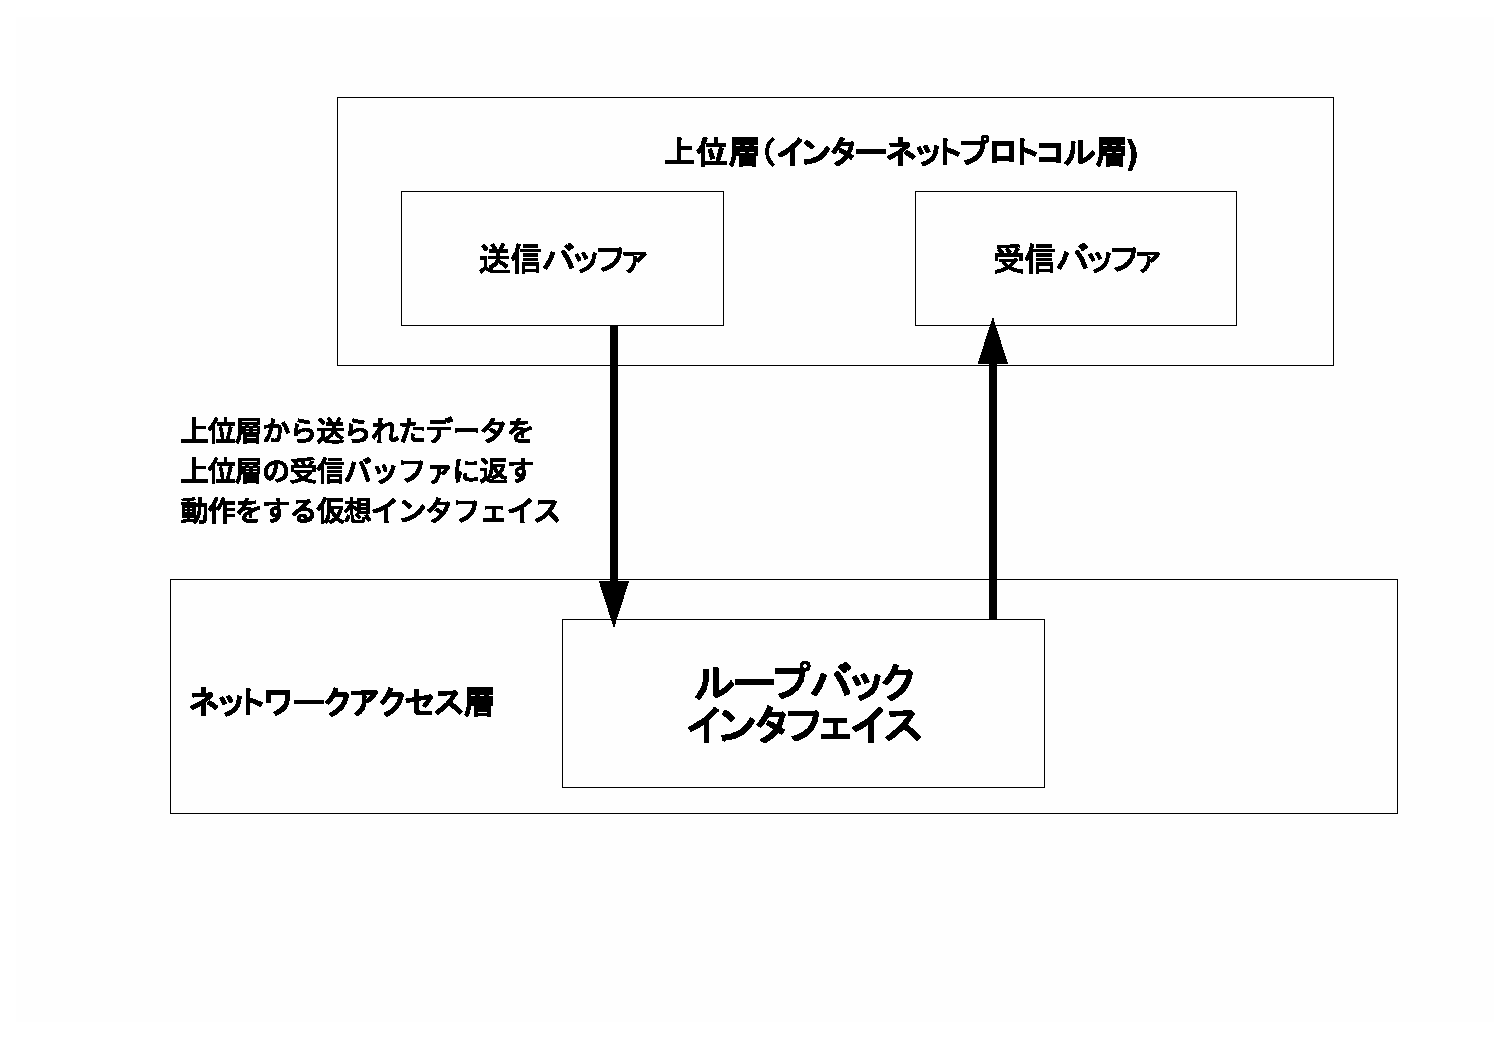
\includegraphics[width=12cm,clip]{draw/loopback.eps}
	\caption{ループバックインタフェイス}
	\label{fig:loopback}
\end{figure}

本章の最後に、仮想的な一対一通信のインタフェイスである、ループバックインタフェイスを説明しよう。では、ループバックインタフェイスは、何と何の間の通信のインタフェイスなのだろうか。

ループバックインタフェイスは、自分と自分の通信のためのインタフェイスである。

ループバックインタフェイスは、ネットワークアクセス層がインターネットプロトコル層に対して提供する、仮想的なネットワークいたフェイスである。

ループバックインタフェイスは、ループバックインタフェイス宛に送信されたデータを、そのまま自分自身のインターネットプロトコル層に、「受信したデータ」として渡す、それによって、物理的なインタフェイス、ネットワークを介さずに、自分自身とインターネットプロトコル層レベルの通信が可能となる。

つまり、同一ホスト上で動作しているアプrケーション間で、TCP/IPによるプロセス間通信が可能となるということだ。

ループバックインタフェイスは実在するインタフェイスと派対応していない。そのため、MACアドレスなど、物理デバイスと対応づけるための名前をもたない。\footnote{ifconfigコマンドでループバックインタフェイスの情報を見ると、MACアドレスは設定されていないことがわかる。}

\chapter{ネットワークアクセス層(その2) 複数の端点を結ぶネットワーク}



ネットワークとは、共有する通信路を介して、相互に直接通信が可能な端点と、その通信路であるとします。では、複数の端点を結ぶネットワークとはどんなものでしょうか。

ここでは、例外はありますが、「誰かに中継してもらわなくても複数の相手と相互に通信できる範囲」であると考えることにします。
本章では、その考えに基づいて、ネットワークアクセス層で、複数の端点を相互に接続するネットワークについて説明をしていきます。


\section{複数の端点を結ぶネットワーク}
複数の端点を結ぶネットワークの特徴は、一対一のネットワークの特徴と全く逆である。自分以外の相手に、区別してもらうための名前なりアドレスなりを全ての端点が持っている。

そして、宛先としてそのアドレスもしくは名前を使い、複数の端点が共有する通信路の上で、特定の相手と通信を行う。

\subsection{ブロードキャストとマルチキャスト}
複数の端点を結ぶネットワークを考えるとき、一対一のネットワークにはない概念が登場する。それは、データの送信先の、その宛先を指定する方法として、ブロードキャストとマルチキャストという概念が現れることである。

ブロードキャストは、同じネットワークの中に接続された端点全てが受信しなければならない通信である。これは、宛先にかかわらず全ての受信者が受信し、処理しなければならない。そのため、一斉放送という意味でブロードキャストという名前が付けられている。

マルチキャストは、同じネットワークの中に、それを受信する必要がある端点が複数ある場合の通信である。受信する側は、宛先のマルチキャストアドレスを参照して、自分が受信しなければならない場合のみ受信し、処理を行う。

最もこれらの概念は、ネットワークアクセス層に固有のものではない。次章以降で説明する、インターネットプロトコル層でも、同様の会年を用いる。だが、ネットワークアクセス層のそれと、インターネットプロトコル層のそれを区別するよう、注意したい。

\section{イーサネット}

では、複数の端点を結ぶネットワークの代表格であり、現在ではLANを構成する規格としてどこででも使用されているイーサネットについて解説しよう。

イーサネットは伝送媒体にケーブルを使用する方式、つまり有線である。だが、イーサネットの技術はALOHAという、無線によるデータ通信技術を基にしている。そのため、無線通信であったことに由来する性質や問題がある。なにより、イーサネットのトラブルはそれを理解していないからこそ「発生させてしまう」ことが多い。

\subsection*{}
\begin{itembox}[l]{いもうとコラム イーサネットの歴史}
まずは、イーサネットの大まかな歴史を追いかけてみましょう。イーサネットの起源までさかのぼれば、その歴史は1960年代後半のハワイ大学にはじまります。

\begin{description}
\item[1960年後半]ハワイ大学で、イーサネットの原型であるALOHA-netの構築が行われました。このALOHA-netは無線ネットワークでした
\item[1972年]XeroxのPARCでロバート・メトカーフがALTO ALOHAネットワークの実験を行いました。これが初のイーサネットの実装です。ALTO ALOHAは、PARCで開発されていたALTOのネットワーク構築に用いられました。通信速度はALTOのクロックに準拠した2.94Mbps\footnote{ALTOのベースクロックが5.88MHzでした}
\item[1973年]メトカーフによって、はじめてEthernetの名称が用いられました同年、特許出願
\item[1976年]メトカーフがNCC(National Computer Conferende)でイーサネットの概念を発表
\item[1977年]イーサネットの特許を米国で取得
\item[1978年]イーサネットリピータの特許を取得。このときまではイーサネットはXeroxの独占でした。
\item[1979年]DEC,Intel,Xeroxの三社がDIX仕様を公開。Xeroxが特許を開放しました。このときの速度は10Mbps
\item[1980年]DIX仕様をベースに、IEEEにEthernet1.0として提出
\item[1985年]IEEE802.3 Carrier Sense Multiple access with Collision Detection(CSMA/CD) Access Method and physical Layer Specification策定。同年、802.3aとして10Base2シンイーサネットと802.3c 10Mbpsリピータの規格も策定されました。
\item[1990年]IEEE802.3i 10BaseT策定
\item[1995年]IEEE802.3u 100BaseT及びAuto Negotioation策定
\item[1999年]IEEE802.3ab 1000BaseT策定
\end{description}

\end{itembox}


\subsection{ALOHA}

イーサネットの歴史的経緯をひもとくと、必ずALOHAという無線ネットワークの名称が出てくる。このALOHAを有線化したのが、最も初期のイーサネットである。では、最初にALOHAがどのようなネットワークであったかの説明を行なおう。

ALOHAとは、1960年代後半から1970年代前半にかけて構築・運用された、ハワイ諸島に分散設置されたハワイ大学の施設と中央のホストコンピュータを結ぶネットワーク、ALOHA-netで使用された方式である。\footnote{ネットワークの直径400Kmであった}当時のハワイは電話線の品質が低く、専用ケーブルを引く費用は莫大であったため、無線によるネットワークが構築された。

ALOHA-netでは、全ての拠点で同一の無線周波数を使用した。そのため、複数の拠点が同時に電波を出したときに発生する混信を回避する制御が必要となることが判明し、それが機能として実装されていった。つまり、同一の伝送媒体を複数の端点が共用するネットワークであったわけだ。

では、そのALOHAの進化の過程についてk、簡単に説明していこう。

\subsection{pure ALOHA}

一番最初に、ALOHA-netの通信方式として実用化されたものを、特にpure ALOHAという。pure ALOHAの通信手順は、以下のような簡単な者である。

\begin{enumerate}
\item 送信者は任意のタイミングでパケットを送出
\item パケットを正常に受信したら、受信者は、受信完了を伝える符号のACKを送出
\item 一定時間内にACKが戻らなければ送信者は再送出
\end{enumerate}
送信タイミングは完全に任意であり、他のホストが送信を行っていても、とりあえず送信を開始してしまう。そのため、混信が多く発生した。そのため、単位時間で有効なデータを送信できるという意味のスループットは 18%程度であった。\footnote{つまり、混信による時間消費、再送などに82%が消費されていたことになる。}

\subsection{改良型ALOHA}

ALOHAの運用によって、単一の無線周波数を複数の拠点からの送受信に使用する、つまり、共有の伝送路を複数の拠点が使用するには、その利用を制御する必要があることが判明した。ALOHAの改良についても簡単に説明しよう。

\subsubsection{Slotted-ALOHA}

ALOHA-netの通信効率を改善するために、時分割したスロットを単位としてデータを送出するSlotted-ALOHAが登場した。これは、同期した時計を使い、送信可能な時間枠をスロットとして管理する。それによって、衝突したスロットのデータを特定し、それだけ再送すればよいようにした方式である。\footnote{時間によって送信できるノードを制限する方式ではない。あくまで、衝突したデータの切片を明らかにするために時計を用いただけである。}Slotted-ALOHAによって、ネットワーク利用率が36\% まで向上した。

\subsubsection{r-ALOHA}

Slotted-ALOHAの改良としてr-ALOHA(reservation-ALOHA予約ALOHA)という方式ができた。これは予約情報を先行して送信し、それを受信した他ノードは送信を行わないという方式である。送信を行う拠点は、予約に成功したのを確認してから送信する。予約の確認とは、予約後一定時間他のホストが電波を出さなかったことを確認することである。その後、送信を行う拠点はパケット送信を開始する。

この方式は、予約を行い、その成功を確認するというオーバヘッドがある。だが、それは確率的に発生する混信で失われる時間よりも小さい。

その後更に、ALOHA-Reservationという予約方式を改良したALOHAも運用されている。だが、本書ではそのような改良が行われたという記述に留めることにする。

\subsection{ALOHAとはどんな通信方式であったのか}

ここで、ALOHAとはどのような通信方式であったか、それを見直してみよう。

\begin{itemize}
\item 伝送媒体を共有する。単一の終発数の電波を使用するので、どこかが送信中は、伝送媒体を専有させる必要がある。
\item 自分が送信したパケットは、自分に返ってこない\footnote{理想環境での話なので、地形や電離層で反射することは考えない。}。つまり伝送路におけるループは存在しない
\item 送信は、全ての拠点で受信可能である。一対一の通信路を確保しない。逆に全ての拠点は伝送路を常時監視する、つまり常時受信待ちを行い、何かパケットが受信できた場合、自分宛化を判別する。自分宛でない場合はその場でパケットを捨てる。
\item 送信する側は、受信する側に事前の連絡は行わない。受信する側が受信することを期待するのみである。
\end{itemize}

これらのアイディアを有線のネットワークに持ち込んだのが、メトカーフであり、次に説明するALTO ALOHAの実装である。

\subsection{ALOHAからALTO ALOHA、そしてイーサネットへ}

現在の、UTP(Unshielded Twist Pair 遮蔽なし撚り対線)とHUBを使用するイーサネットからは、無線通信を祖とした姿をイメージするのは困難である。イーサネットの祖が無線通信であった歴史を見るために、最初のイーサネット実装であるALTO ALOHAまで戻ることにしよう。

1972年、ロバート・メトカーフは、空中に電波を流すかわりに、電気信号の伝送に使用する同軸ケーブルを伝送媒体とした、有線のALOHAネットワークを構築する。当時はまだイーサネットという名前ではなく、パロアルト研究所のコンピュータ、ALTOを結ぶALOHA方式のネットワークということで、ALTO ALOHAという名称が付けられた。

同軸ケーブルとは、電気信号を伝送するケーブルである。身近なところではテレビのアンテナ線に使われているので、目にしたり取り扱ったりすることも多いであろう。構造を簡単に説明すると、中心に信号を伝送する内部胴体があり、その周りにポリエチレンなどの絶縁体がある。その外部にメッシュ状の外部導体、一番外側がビニールなどの保護皮膜となる。外部導体がシールドとなるので、外のノイズが内部導体に乗ったり、内部導体の信号が外に向けて放出されにくい構造となっている。

ALTO ALOHAの伝送媒体は、両端にターミネータをつけた1本の同軸ケーブルであった。ターミネータとは、終端抵抗器と呼ばれることもある電気素子である。ケーブルの端に達した電気信号が反射して、ケーブルの中を戻っていかないように、エネルギーを消費させる役目を持つ。\footnote{無線通信では、試験のためにアンテナと同様の電気抵抗を持つが、電波を発射しないダミーロードと呼ばれる抵抗器を用いることがある。これも、原理と目的はターミネータと同様である。ターミネータがない場合は、開放端から信号が電波として飛んでいったり、反射してケーブルの中を帰ってきたりする。}わかりやすくいうと、信号の発信者から見たときに、理想的な空中のように、送信した信号が自分のところに戻ってくることがない伝送媒体を用意した。

では、各ホストから伝送媒体である同軸ケーブルには、どのように接続するのだろうか。ALTO ALOHAでは、同軸ケーブルの内部導体を伝送媒体として信号を送受信する装置、トランシーバを、同軸ケーブルに直接取り付けた。このトランシーバが、コンピュータと接続され、同軸ケーブルの上を流れる信号を受信し、同軸ケーブルに対して信号を送信した。

ALTO ALOHAがEthernetという名称になるのは、翌1973年のことである。
このALTO ALOHAの構造が、そのままイーサネットの基本原理として40年近く使い続けられていくこととなる。

\begin{figure}[htbp]
	\includegraphics[width=12cm,clip]{draw/altoaloha.eps}
	\caption{ALTO ALOHAの概念図}
	\label{fig:altoaloha}
\end{figure}

\subsection{トランシーバ}

ALTO ALOHAにおけるトランシーバ(Transciever)とは、どのような装置なのであろうか。その答えを先に書いてしまえば、ALTO ALOHAのトランシーバは、同軸ケーブルに対して、信号の送信と受信の両方が可能な装置という意味である。

トランシーバという言葉で、無線通信用の手持ちの無線機を思い浮かべる人も多いであろう。このように、トランシーバという言葉に、なんとなく「無線でお互い話ができる機械」というとらえ方をしている人も多いと思われる。そこで、トランシーバについて簡単に説明をしよう。。

トランシーバ(Transciever)という言葉は、送信機と受信機(Transmitter-Reciever)の合成語である。その意味は、送信機と無線機が一つの箱に入った機械、ということである。

もともと無線機は、送信機と受信機が分かれていた。それだと持ち運びに不便ということで、送信機と受信機を一つの箱に入れるようになる。そうすると、送信機と受信機の両方に存在する、電源系やチューナーなど、一部の電気回路の共用も可能となった。そうして、送信と受信の両方ができる機械として、トランシーバが成立したという経緯がある。だが、送信機能と受信機能は基本的に別回路として構成され、同じ箱に入っているにすぎない。

\subsection*{}
\begin{itembox}[l]{いもうとコラム イーサネットという名前}
Ethernetという名称は、共有伝送媒体を、真空中で電磁波を伝播する仮想の媒体「エーテル」に見立てた名称です。物理メディアが全てのホストにビット列を伝播する様子が、光の伝播媒体であるとされたluminiferous etherと同じであるとして、イーサネットという名前がつけられました。

イーサはエーテルの英語読みです。なお、エーテルの存在は現在では否定されています。電磁波の伝送媒体としてのエーテルの存在を否定したのが、有名なマイケルソン・モーリーの実験です。つまり非実在(ry
\end{itembox}

\section{イーサネットにおける共有伝送媒体の制御}

ALOHAでは、共有する伝送媒体、つまり、同じ周波数の電波をどう管理し、複数の拠点が同時に送信する「衝突」を回避するか、それが改良の歴史であった。では、イーサネットでは、ALOHAの知見と成果をどのように取り入れたのだろうか。

イーサネットでは、共有する伝送媒体である同軸ケーブル、に二つ以上のホストが同時に信号を出さないようにする、「調停」を行う。その調停方法は、CSMA/CD(Carrier Sense Multiple Access/Collision Detect キャリア検知多重アクセス/衝突検出)という名前である。では、CSMA/CDはどのような手順で調停をするのだろうか。。

ここからの説明では、一度に送信される一連の信号を、フレームと呼ぶことにする。イーサネットを流れる一連の信号は、イーサネットフレームと呼ばれる。

\begin{enumerate}
	\item データを送信する前に、伝送媒体上に、最短4マイクロ秒、最長9.6マイクロ秒の信号を送信するだけの時間、信号が流れていないことを確認する。これは、 10Mbpsで、40ビット~96ビットを送出する時間に相当する。
	\item 信号が流れていなければ、伝送媒体に信号を発信する。
	\item 伝送媒体が使用されていないときに信号を送る権利は、全てのホストで等しい。優先順位はないし、特権的に調停を行うノードも存在しない。  \item 信号を送信するホストは、送信中を含む常時、伝送媒体を監視する。他の信号と衝突した場合は、直ちに送信を中止する。その際JAM信号と呼ばれる特別な信号送信して、各ホストに現在受信したフレームを破棄するよう通知する。
	\item JAM信号送出後、ランダムな時間待ったのちに再度送信を試みる
\end{enumerate}

イーサネットでは衝突は必ず発生する。これは異常な状態ではなく、共有の伝送媒体状を有限の速度の電気信号が伝播していくので、タイミングによっては「信号が届いていない」状態と、送信しているホストがいない状態が区別できないためである。

衝突が発生した後ははランダムな待ち時間の後に再送信を試みる。そうすることで、次回以降衝突が発生する確率を下げることができる。

CSMA/CDにおいて、Collision Detectという用語は、ALOHAに由来する問題とその解決方法を正直に説明している。だが、それ故に過去ではイーサネットの性能に疑問の余地を与えていた面もある。\footnote{オライリーの「詳説イーサネット」の筆者であるCharles E. Spurgeonは、その誤解を避けるためには、「調停(arbitation)」という用語を使うべきと記している。}



\subsection{衝突の検出とケーブルの総延長・最小フレームサイズ}

\begin{figure}[htbp]
	\includegraphics[width=12cm,clip]{draw/colision.eps}
	\caption{衝突の検出}
	\label{fig:colision}
\end{figure}


伝送媒体である同軸ケーブル上を伝播していく信号は、有限の速度で、トランシーバの接続されている位置からケーブルの両端に向けて進行していく。上記の通り、信号が届いていない状態と送信しているホストがない状態を区別できない。そのため、あるホストがフレームを送信しているときに、他のホストがそれと衝突するフレームを送信することが起こる。繰り返すが、これは障害ではなく、イーサネットでは確率的に起こりうることである。

では、衝突が発生した際に、その衝突を、その原因となったフレームを送出した複数のホスト\footnote{二つのホストからのフレームが衝突するのではなく、二つ以上のホストからのフレームが衝突する。}が検出(Collision Detect)できる条件を考えてみよう。

まず、同軸ケーブルを伝播する電気信号は、注入された点から、両端に向けて光速以下の一定の速度で進行する。この注入された点とは、トランシーバの取り付け位置になる。電気信号の早さは、内部導体に銅を使う同軸ケーブルで、およそ光速の7割とされる。

電気信号が同軸ケーブルを伝わっていく様子は、波の進行をイメージするとよいだろう。\footnote{ALOHAとイーサネットを比較すると、電気信号か電磁波かという違いだけで、どちらも波である} また、波の合成は単純に足し算である。つまり、二つ以上のフレームが衝突すると、その電気信号は、その二つ以上のフレームの波を合成した、「異常な」波形となる。

イーサネットでは、フレームを送信する側は、フレームの送信開始から送信完了までの間、衝突が発生するかしないかを監視する。送信側が衝突の発生を検知できるのは、別のホストが送出したフレームの先頭が、自分が送信している間に届くことで、自分が送信している信号と同軸ケーブル上の信号が一致しない状態になるからである。

送信開始から送信終了まで衝突が起こらないという状態は、フレームが最も遠いところ\footnote{ここでいう最も遠いところとは、同軸ケーブルの長さで考える。純粋に、伝送路の物理的な距離である。}まで伝播するまで、他のすべてのホストが全く送信しないということである。そして、最悪のケースで衝突が起こった状態というのは、フレームが送信したホストから最も遠いホストのトランシーバに伝播する直前に、送信したホストから最も遠いところにあるホストが送信を始めてしまうことである。この最悪のケースで双方が衝突を検知するには、自分が送信したフレームの先頭が、衝突するフレームを送出した相手に届くまでの時間の、倍の時間が必要である。これは、自分が送出したフレームが相手に届くまでの時間と、その信号が到着する直前という最悪のタイミングで相手が送出した信号が自分に届くまでの時間の合計である。

それだけの時間かかって検知できる「最悪のタイミング」の衝突を検知するにはどうすればよいだろうか。それは、自分が送出した信号が、最も遠い位置にいる相手に届くまでの時間の倍の時間、フレームを送出し続けることである。そうすることで、最悪のタイミングで送出された、衝突するフレームの信号と、自分が送出したフレームの信号が合成されて、異常な信号が発生していることで、衝突を検知できる。これを図示したものが、図\ref{fig:colision}である。

ここまでの話で予想がついたかもしれないが、フレームの最小サイズ、フレーム送出時のビット送信速度、、同軸ケーブルの総延長の三つのパラメータは、相互に影響しあう関係にある。フレーム送出時のビット送信速度は、イーサネットの規格ごとの通信速度となる。また、フレームの最小サイズは、互換性維持のために過去の規格と同一の、固定パラメータである。\footnote{GbE以上の規格では、フレームの最小サイズを古い規格にあわせると、ケーブル長が短くなりすぎる。そのため、ジャンボフレームという巨大なフレームを導入することで、ケーブル長を稼いでいる。}そのため、イーサネットのそれぞれの規格では、通信速度で最大のケーブル長が決まると考えて良いだろう。

\subsection{半二重と全二重}

\begin{figure}[htbp]
	\includegraphics[width=12cm,clip]{draw/duplex.eps}
	\caption{半二重と全二重}
	\label{fig:duplex}
\end{figure}

ここまでに説明したCSMA/CDは、同じ衝突ドメインで、あるホストが送信していると、他のホストは受信しかできない。この状況を単純にするためにホスト2台からなるネットワークで考えてみよう。この場合、片方のホストが送信している間は、もう片方のホストは受信しかできない。同時に送信しようとすると、「衝突」が発生する。

このように、二つのホストが相互に通信できるが、送信はどちらかしかできない通信方法を、半二重(half-duplex)という。つまり、片方が送信しているときは受信、というように、送受信を交代して通信を行うわけだ。

HUBとホストの接続を説明した際、、ホストのTDとHUBのRD、HUBのTDとホストのRDが接続される信号交差が行われている。信号交差を行っているということは、それぞれ信号の伝達をする方向が決まっている、いわば、「上り」と「下り」の経路が別々に存在する。そこで、「経路が別なんだし、送信と受信を同時にやってもいいんじゃね?」というアイディアに繋がった。このような、送信と受信を同時に行う通信方法を、全二重(full-duplex)という。

全二重は、二つのホストが一対一で接続して通信する場合のみ成立する。便宜上、このホストにAとBという名前をつけて説明していこう。AからBに信号を送る経路と、BからAに信号を送る経路が、それぞれ別に存在しなければならない。また、このAとBの間の経路を、第三のホストCと共有することはできないということである。。

では、一対一で、送信と受信の線が別々にあると、イーサネットではどんな利点があるのだろう。それは、CSMA/MDでいうところの「衝突」が発生しなくなる。つまり、CSMA/CDによる制御を行う必要がなくなるということである。

また、全二重方式では、AからBへの送信と、BからAへの送信を同時に行うことができる。実効的に、表記された通信速度の倍で通信することが可能となる。たとえば、100BaseTXというイーサネットの規格では、全二重方式を用いることができる。その場合、AからBへの送信とBからAへの送信で、それぞれ100Mbpsで通信することが可能となる。つまり、単純に計算すれば200Mbpsで半二重通信しているのと同じになる。

繰り返すが、イーサネットで全二重方式を実現するには二つのホストの間で一対一の通信を行わなければならない。つまり、衝突ドメインが存在してはならない。つまり、全二重はスイッチングHUBのみでサポートされる。また、伝送媒体で、送受信の往復には別の経路が存在しなければならない。

逆に、全二重方式のみで構成されたネットワークは衝突ドメインが存在しないと言うこともできる。これは、接続された機器が全て一対一通信を行い、送受信の往復に別の伝送経路を使用するということである。つまり、ALOHAに由来するイーサネットの基本、複数の機器が共有して使用する伝送媒体というものが存在しなくなることである。



\subsection*{}
\begin{itembox}[l]{いもうとコラム 全二重と半二重のマッチング}
現在では、イーサネットのネットワーク機器を相互に接続した場合は、全二重、半二重のマッチングは、多くの場合自動で行われます。そのため、全二重、半二重を明示的に指定しなければならない場面はあまりありません。また、多くの場合は、機器が自動で全二重の通信を選択します。

ですが、業務用のネットワーク機器など、手動で明示的に全二重と半二重どちらを使うか設定することができる機器も、多く存在します。

では、自動で行われるマッチングが失敗したり、手動での設定を間違えて、ホストの一方が全二重、もう一方が半二重で通信しようとした場合は、何が起こるのでしょうか。

全二重と半二重のミスマッチングが発生している場合、はっきり分かる現象として、通信が遅くなります。\footnote{接続したネットワーク機器間の通信が異常なレベルで遅い場合は、全二重、半二重のネゴシエーションの失敗や設定ミスを疑ったほうがいいでしょう。}これは、片方がCSMA/CDに従って通信を行っているのに対し、もう片方がCSMA/CD手順関係なしに送信を行うためです。

そのため、半二重側から見たとき、衝突の発生頻度が高くなります。その結果、通信速度が遅くなるというわけなのです。

一方、全二重側から見ると、通信の相手は高い確率で通信の中断を求めるJAM信号を送信してくるように見えます。そのため、確率的に、単位時間内で成功する送信が減り、結果、通信速度が遅くなるというしくみです。\footnote{実際には、トランスポート層の応答待ちなどで、イーサネットで通信が遅くなることがトリガーとなって、雪達磨式にアプリケーション層の通信の遅延の原因となっていきます。}
\end{itembox}





\section{イーサネットでホストを区別する}

\begin{figure}[htbp]
	\includegraphics[width=12cm,clip]{draw/macaddr.eps}
	\caption{MACアドレスの構造}
	\label{fig:macaddress}
\end{figure}

本章の冒頭で、複数の端点が通信経路を共有するネットワークでは、端点を区別するための名前もしくはアドレスが必要になる、という話をした。では、イーサネットでは、どのようにお互いを区別しているのだろうか。

イーサネットは、一つのホストが送信した信号を、全ホストで受信し、自分宛でないフレームは破棄するというALOHA以来の方法で、特定の宛先にフレームを届けている。そのため、イーサネットでは、共有の伝送媒体に接続されたホストを区別する方法が必要になる。

その区別を行うのに、MAC(Media Access Control メディアアクセス制御)アドレスという48bit(6octet)長のアドレスを使用する。このMACアドレスは、イーサネットのフレームを送受信する全てのインタフェイスに、世界唯一のユニークなものとして割り当てられる。つまり、ネットワーク内で重複することがない。そのため、イーサネットのプロトコルには、ホストのインタフェイスにMACアドレスを割り当てたり、同じネットワーク上のMACアドレスを管理したりする仕組みがない。



MACアドレスの構造は、図\ref{fig:macaddress}のように、48ビット長のアドレスである。
MACアドレスはネットワークインタフェイス毎にユニークであり、上位24ビットがベンダに割り当てられたOUI(Organizationally Unique Identifier 管理組織識別番号)となる。このOUIは、ベンダコードと通称されることが多い。また、下位24ビットが、ベンダがネットワークインタフェイスに割り当てるアドレスとなる。

MACアドレスには、同じ同軸ケーブルに接続されているの全てのホスト宛を意味するブロードキャストアドレスと、その中で特定のグループをつくり、グループに属するホスト全てのみを宛先とするマルチキャストアドレスとがある。これは、上位層のブロードキャストアドレス、マルチキャストアドレスとは別のものである。

\subsection{イーサネットの通信手順}

イーサネットでの通信手順を、MACプロトコルという。このMACプロトコルが、前述したCSMA/CDとMACアドレスを使用して、どのような手順で行われるかを説明しよう。
\begin{enumerate}
\item ホストは、通常は共有通信チャネルを監視する。共有通信チャネルとは、同じネットワークを構成するための伝送媒体である。
\item あるホストが送信するときは、前述のCSMA/CDの手順で行う。
\item 共有通信チャネルに送り出されたイーサネットフレームがあれば、とりあえず受信する。その後、宛先を自分のMACアドレスと比較、同じであればヘッダとフッタを抜いたデータ部分を上のレイヤに渡す。自分のMACアドレスと一致しなければ、そのフレームは無視する。
\end{enumerate}

MACプロトコルの動作は、これだけしかない。イーサネットでは、同一の伝送媒体にフレームを送信し、同一の伝送媒体に接続されている全てのホストで受信する。その後、自分宛でないデータは破棄するという手順である。

イーサネットは、送信が全てのホストで受信可能であることから、ブロードキャスト型の通信と言われることがある。

また、イーサネットでは、エンドツーエンドの通信路を確保したり、受信の確認を送出したりはしない。イーサネットでは、相手が受信したことを期待するだけである。確実な通信を行う必要があれば、上位層のレイヤが、イーサネットを通信手段に使って行うであろう。そして、TCP/IPにおいて確実な通信を行うために何かをするのは、トランスポート層のTCPだけである。イーサネットなど、ネットワークアクセス層の仕事ではない。


\subsection{MACアドレスのブロードキャストアドレス}

MACアドレスには、ブロードキャストアドレスと呼ばれる特別なアドレスがある。ブロードキャストアドレスは、そのネットワークに接続された、全てのインタフェイスを宛先とする。\footnote{インターネットプロトコル層にもブロードキャストアドレスが存在する。それは、ここで説明するMACアドレスのブロードキャストアドレスとは全く別のものである。}MACプロトコルの手順で、全てのホストは、送出されたフレームをいちど受信する。そのフレームの宛先がブロードキャストアドレスであれば、そのフレームは自分宛として処理する。

つまり、ブロードキャストアドレスは、同じネットワークに接続された全てのインタフェイスが受信する宛先アドレスである。ブロードキャストアドレスは、MACアドレスの全てのビットを1にしたものであり、十六進表記するとFF:FF:FF:FF:FF:FFとなる。

ブロードキャストアドレスは、宛先としてのみ指定可能である。送信元MACアドレスとして使用することはできない。

\subsection{MACアドレスのマルチキャストアドレス}
MACアドレスには、マルチキャストアドレスとよばれるアドレスもある。マルチキャストアドレスは、同じネットワークの中で、受信する必要のあるネットワークインタフェイスのみが受信するアドレスとである。。

マルチキャストアドレスは、先頭16bitが、00110011-00110011、つまり16進で33-33となる。

ブロードキャストアドレスと同様に、送出されたフレームは、MACプロトコルに従って、全てのホストに到達する。そして、その宛先アドレスが、自分に似設定されたマルチキャストアドレスであれば、そのフレームを受信する。それが自分に設定されたマルチキャストアドレスでないばあいは、破棄する。

マルチキャストアドレスも、ブロードキャストアドレス同様、送信元MACアドレスにすることはできない。

\subsection{ブロードキャストアドレス、マルチキャストアドレスの区別}
ブロードキャストアドレス、もしくはマルチキャストアドレスを宛先としたフレームは、とりあえず全てのホストのいたフェイスに到達する必要がある。つまり、同じネットワークの中にある中継機器は、それを見分けて中継しなければならない。

ブロードキャストアドレス、マルチキャストアドレスとも、MACアドレスの先頭バイトの最終ビットが1である。ネット枠アクセス層に対応した機器は、それを判別して、全てのインタフェイスに中継をする。

\section{イーサネットの接続と衝突ドメイン}

\begin{figure}[htbp]
	\includegraphics[width=12cm,clip]{draw/collisiondomain.eps}
	\caption{衝突ドメイン}
	\label{fig:collisiondomain}
\end{figure}

ここまで、イーサネットは同軸ケーブルを使用していた、という説明を行っていた。つまり、同じ一本の同軸ケーブルに繋がっている全てのホストが、一つのネットワークを構成しているということである。これは、一本の同軸ケーブルが、「どのネットワークか」という、ネットワークを区別する単位であると言うこともできるであろう。

では、ネットワークを区別する単位である同軸ケーブルが複数あった場合はどうなるだろうか。そして、その複数のネットワークを接続していくことを考えたら、何が起こるであろうか。

同軸ケーブルが複数ある、つまり、ネットワークが複数ある場合に、ネットワークアクセス層のレベルで接続して、一つのネットワークにする方法について説明する。この複数のネットワークの接続を考えるときに出てくるのが、衝突ドメイン(Collision Domain)という概念である。この衝突ドメインは、どのように定義されるのだろうか。

衝突ドメインとは、同じ共有通信チャネルに接続されたホスト全てである。また、その中の一台が送信している間、同じ衝突ドメインになるホスト全てが、CSMA/CDによる調停に従って送信できなくなる。つまり、同じ衝突ドメインに属する複数のホストが同時に送信すると、衝突が発生する

イーサネットにおいて、同じ同軸ケーブルに接続されている、同一のネットワークのホストは、同じ衝突ドメインに属していると言うこともできる。

\subsection{複数の衝突ドメインを接続する}




では、次に、複数の衝突ドメイン、つまり、同軸ケーブルからなるネットワークを相互接続することを考えてみよう。

二つのネットワークを接続する機器は、その機能の違いから二種類存在する。その機器はそれぞれ、リピータ、ブリッジと呼ばれている。リピータとブリッジは、どちらも、二つのネットワークに接続して、接続したネットワークの間で、フレームを中継する機器である。

では、二つのネットワークの間でフレームを中継する、という機能では同じなのに、なぜリピータとブリッジの二種類の機器があるのだろうか。実は、リピータは増幅器として電気的にフレームの信号を中継する機器であり、ブリッジは二つのネットワークに同時に接続してフレームを転送するコンピュータである。このように、フレームを中継するという機能は同じでも、中身が全く異なる機器なのだ。

では、リピータとブリッジについて、もう少し説明をしていくことにしよう。

\subsection{リピータ}

二つのネットワークを、単純に接続して、ひとつの同じネットワーク「するための機器を、リピータ(中継器)という。

接続したネットワーク片方のネットワークでフレームの送信があり、そのフレームがリピータに届いたら、リピータによって、そのままもう片方のネットワークにも伝送される。だが、受信した電気信号ものをそのまま流すのではなく、イーサネットフレームとして再度送り出す。単純に内部でケーブルを接続しているだけではない。

リピータで接続された二つのネットワークは、同じ衝突ドメインとなる。また、ケーブルの総延長という観点で見ると、リピータによる接続は、同軸ケーブルを継ぎ足すのと等価である。

\subsection{ブリッジ}

ブリッジは、二つのネットワーク、つまり、衝突ドメインに同時に接続されるコンピュータである。ブリッジは、中継するフレームの送信元MACアドレスを参照して、それぞれの衝突ドメインにどのMACアドレスをもつインタフェイスが接続されているかを学習する。

ブリッジは、学習したMACアドレスの一覧を持つ。このMACアドレスの一覧は、宛先となる機器が二つあるどちらのネットワークに接続されているかを判断するのに用いられる。フレームの宛先が送信したホストと同じネットワークであれば、ブリッジはフレームをもう一方のネットワークに転送しない。宛先が、送信したホストと違う方のネットワークにあることがわかっている場合、もしくは、そのMACアドレスがまだ一覧表になくて、宛先がどちらのネットワークにあるかわかっていない場合は、ブリッジはフレームをもう一方のネットワークへ転送する。

学習が進んで、それぞれのネットワークに接続されたインタフェイスのMACアドレスをすべて学習したら、違うネットワークにあると分かっているフレーム、もしくはすべてのインタフェイスに届けるフレーム以外は、ブリッジで中継されることがなくなる。

そのため、ブリッジに接続された二本の同軸ケーブルそれぞれの中で完結する通信であれば、ブリッジによって同じネットワークになったにもかかわらず、衝突せずに同時に通信することができる。

つまり、ブリッジで接続されたそれぞれの部分は、同じネットワークであるが、同じ衝突ドメインではない、独立した二つの衝突ドメインとなる。

\begin{figure}[htbp]
	\includegraphics[width=12cm,clip]{draw/repeaterbridge.eps}
	\caption{リピータとブリッジ}
	\label{fig:repeaterbridge}
\end{figure}

\subsection{ネットワークを接続したときの総延長}

ネットワークをリピータで接続して同一の衝突ドメインとした場合、最も離れているホスト同士の距離を、ケーブルの総延長という。

繰り返すが、イーサネットは、CSMA/CDで同一の衝突ドメインで発生する衝突を検知するために、通信速度によってケーブルの総延長が規定される。では、リピータやブリッジで二つのネットワークを接続した場合、そのケーブルの総延長はどのように考えればよいだろうか。

リピータの場合は、接続したケーブルは、論理的に一本のケーブルと見なすことができる。つまり、接続した全てのケーブルの長さを合計して、そのイーサネットの規格で定められたケーブル長より短くしなければならない。

ブリッジの場合は、少し複雑である。接続されるネットワークは、電気的にはそれぞれ独立している。だが、ブリッジは、有限の速度で動作するコンピュータである、フレームからMACアドレスを読み取り、必要であれば適切なネットワークに転送する処理に、ゼロでない時間が必要である。つまり、ブリッジを介した通信に時間が必要であり、それは、ケーブルの総延長が伸びたことと等価である。

ブリッジ接続の場合は、ケーブルの総延長と、ブリッジを何段まで繋ぐかを同時に考慮する必要がある。

\subsection{ブロードキャストフレームの中継}
先ほど、ブロードキャストアドレスは、同じネットワークのホスト全てを宛先としたMACアドレスであると説明した。つまり、ブロードキャストアドレス宛のフレームは、同じネットワークに接続された全てのインタフェイスに届く必要がある。

リピータは、二つの衝突ドメインを連結している。そのため、ブロードキャストアドレス宛を含む全てのフレームは、リピータで接続された、ネットワーク全てに伝播する。

ブリッジは、二つの衝突ドメインを独立した衝突ドメインとしたまま、同じネットワークとして接続する。だが、これまで書いたように、ブロードキャストアドレス当てということは、同じネットワークの全てのホストにフレームが届く必要がある。
そのため、ブリッジは、ブロードキャストアドレス宛のフレームは、全ての衝突ドメインに対して送出する。そうすることで、同じネットワークのインタフェイス全てに、ブロードキャストアドレス宛のフレームが届く。

\subsection{マルチキャストフレームの中継}
マルチキャストフレームが発信された場合、ブリッジはどのような動作をするであろうか。

先に説明したとおり、マルチキャストアドレスは送信元のMACアドレスとすることはできない。そのため、ブリッジがマルチキャストアドレスを受信するホストがどこに存在するかを受信することはない。そのため、ブリッジはマルチキャストアドレス宛のフレームを全ての衝突ドメインに対して送出する。

そのフレームを受信するかどうかは、受信するインタフェイスがマルチキャストアドレスのグループに所属するかどうかで決定される。


\section{現在のイーサネット}

ここまでイーサネットの説明を行ったが、一度もHUBを使用した現在のイーサネットの説明をしてこなかった。それは、イーサネットの動作を理解するには、ALOHA方式や同軸ケーブルを使用していた頃の昔話から入らないと納得できない点が多いためである。

では、現在、イーサネットによるネットワークを構築するのに使用されるHUBとは、ここまで説明してきた何なのだろうか。

HUBとは、集めるもの、中心、というように、「何かを集中させる部分」という意味がある。その名の通り、HUBには、複数のLANケーブルが接続される。HUBにもうけられた、LANケーブルを接続するための口を、ポートと呼ぶ。HUBのポートの数は、そのHUBに接続することができるLANケーブルの数でもある。\footnote{古いHUBでは、他のHUBに接続する専用のポートと、ホストに接続するポートの一つが排他利用となっている場合がある。そのため、必ずポートの数だけホストを接続できるわけではない。}ここから先は、、現在LANに使用されるケーブル、UTPをHUBに接続するという、現代のイーサネットを説明していきたい。

HUBという名前で呼ばれる機器は、リピータHUBとスイッチングHUB(SW-HUB)に分けられる。このそれぞれについて説明をしていくことにしよう。
\subsection{リピータHUB}

リピータHUBの内部をここまでに沿って説明すれば、共有の伝送路である同軸ケーブルと、そのケーブルに取り付けていた複数のトランシーバを一つの箱に置き換えたものと考えればいいだろう。LAN ケーブルを接続するポートのどれかから共有の伝送路に向けて送信されたフレームは、全てのポートに送信される。

そのため、リピータによって構成されたHUBというおkとで、リピータHUBという名称で呼ばれる。つまり、リピータHUBによって構成されるネットワークは、同じ衝突ドメインとなる。

\subsection{スイッチングHUB}

スイッチングHUBは、ブリッジが発展したものである。スイッチングHUBのポートは、すべて独立した衝突メインである。つまり、スイッチングHUBには、ポートの数だけ衝突ドメインがある。

そして、そのポートの数だけある衝突ドメインを全て、相互にブリッジで接続している。古い解説では、クロスバー式の電話交換機のような模式図で描かれることもあった。

では、個々の衝突ドメイン間の接続はのように行っているのだろうか。スイッチングHUBは、ブリッジの集合体と言うこともできる。つまり、コンピュータである。そのメモリ上のテーブルに、ポートごとに接続されている機器のインタフェイスのMACアドレス一覧表を、ブリッジとしての学習で獲得する。そして、あるポートへ送信されたフレームは、この一覧表を参照して、受信するインタフェイスが接続されたポートにのみ、そのフレームを送出する。

ただし、スイッチングHUBも、全てのポートにフレームを送信するブロードキャストを行う場合がある。学習していないMACアドレス宛のフレームを送信する場合と、ブロードキャスト、マルチキャストのMACアドレスを宛先とするフレームは、全てのポートに送信される。

\subsection{LANケーブル}

ここまでで、LANケーブルとUTPという名称を同じ本野として使用してきた。そのUTPとは何であろうか。

UTPとは、Unsielded Twisted Pair(遮蔽なし撚り対線)の略称である。

撚り対線とは外部にノイズを出しにくく、また、ノイズの影響を受けにくい。では、撚り対線がノイズの影響を受けにくい理由について、簡単に説明しよう。

一本のケーブルに電流を流すと、その周囲に、右ねじの法則に従った回転磁束が発生する。その回転磁束が電磁誘導をおこし、エネルギーの一部が電磁波として放出される。逆に、電磁波にさらされているケーブルは、電磁波による回転磁束によって、電磁誘導による誘導電流を生ずる。つまり、ケーブルはそれだけでアンテナになる)。これが、ノイズを出すということであり、ノイズを受けるということである。

撚り対線は、流す電流の向きが逆になるケーブル2本を撚りあわせた構造になっている。電流の向きが逆であるケーブルが撚られているので、撚り合わせ毎に、発生する磁束は、打ち消しあう方向で隣り合う。それによって、撚り対線のそれぞれのケーブルから発生している磁束は互いにうち消しあう。

次に、撚り対線が電磁波にさらされている場合、つまり、撚り対線を横切る磁束がある場合を考えよう。この磁束でより対線には誘導電流が生じる。だが、「撚ってある」形状のため、その誘導電流は一本のケーブルの中で、常にうち消しあう方向に生ずる。

それによって、撚り対線はノイズを出しにくく、ノイズを受けにくい。

\subsection{UTPのカテゴリ}

UTPは、2芯で一対と数える撚り対線を、複数パッケージして1本のケーブルにしたものである。UTPの規格はカテゴリの後に数字をつけてあらわす。表記としては、カテゴリをCat.と省略して書くことが多い。

このカテゴリは、単位長の1フィート(約30cm)あたり、何回撚りあわせてあるかで決められる。たとえば、カテゴリ3では1フィートあたり2回撚り合わせる。カテゴリ5では、ケーブルのメーカによっては19から25回撚り合わせている製品もある。

カテゴリ6の製品では、4対の依り対線を内部で分離するイソレータを入れることになっている。余談ながら、Cat5で芯にイソレーターっぽいなにかとして光ファイバが入っているオーディオ用の製品が存在するが、その効果はオカルトの領分である。

また、カテゴリ毎に何対の接続が必要かという規定はあるが、撚り対線を何対使用しているかは、カテゴリの数字が多いからという理由で多くなるわけではない。たとえば、 ISDNの接続に使用されるUTP カテゴリ2は8芯4対のツイストペアをコネクタに接続しなければならない。だが、10BaseTに使用するカテゴリ3は、4芯2対の接続となる。また、カテゴリ5を使用する 

また、100BaseTXは、その通信には4芯2対しか使用しない。だが、カテゴリ5の規格では8芯4線の接続をしなければならない。そのため、イーサーネットで使用するLANケーブルは、ネットワークの規格を理解した上で、その規格に対応したカテゴリのケーブルを選択する必要がある。



\subsection{UTPとSTP}

\begin{figure}[htbp]
	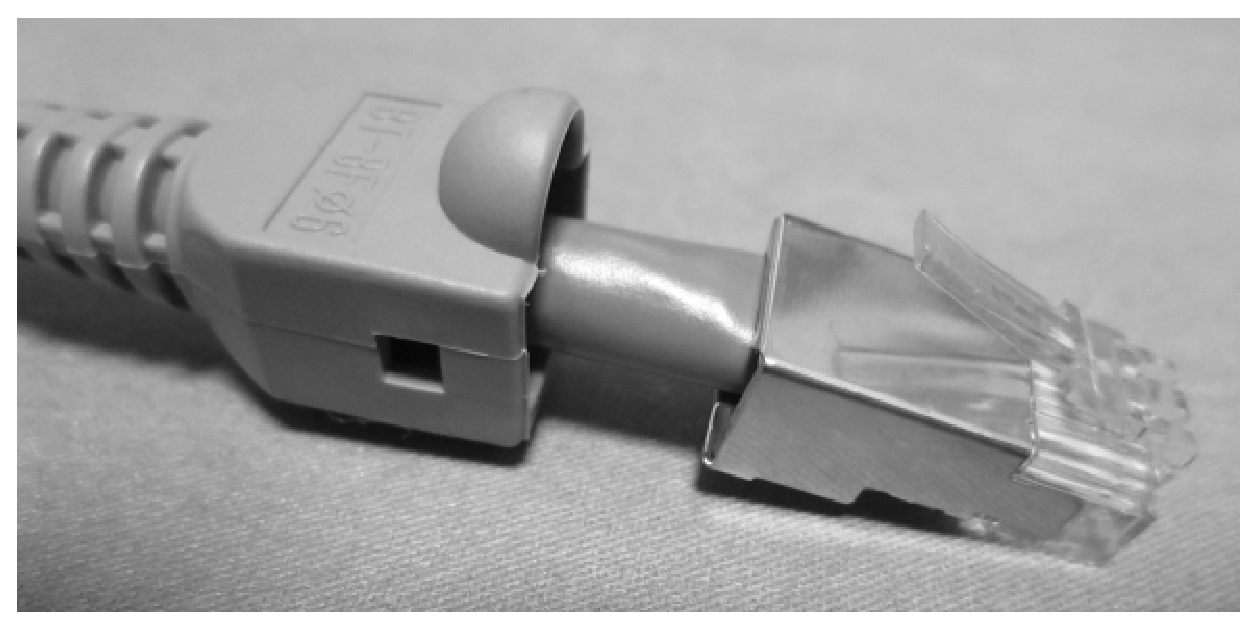
\includegraphics[width=12cm,clip]{draw/stp.eps}
	\caption{STPケーブル}
	\label{fig:stp}
\end{figure}

さて、UTPに関するここまでの説明で、一つ疑問に思わなかっただろうか。撚り対線ならTP(Twisted Pair)でいいのではないか。なぜわざわざUTPと、Unshieldedとつけるのか。

それは、UTPに対してSTP(Shielded TP 遮蔽あり撚り対線)というケーブルが存在するためである。STPは、撚り対線ごとに、同軸ケーブルの外部導体のようなシールドをつけ、よりノイズを受けにくい構造にしたケーブルである。図\ref{fig:stp}でわかるように、コネクタ部分に金属シールドが着いていることがSTPの外見的特徴である。

STPは、特にノイズの多い工場などで使用される。だが、シールドを接地(アース)する必要があるため、ネットワーク機器もSTP対応のものが必要となる。

ヨーロッパで普及している規格であるが、日本では、STP が必要な場面では光ファイバが使用されることが多い。そのため、日本ではSTP対応のケーブルや機器は、あまり見かけることはない。

\subsection{LANケーブルのピンアサイン}

LANケーブルで使用されるRJ-45というコネクタは、8本のピンがある。このピンを2本ずつ接続することで、一対の信号線ができるようになっている。では、実際にLANケーブルの線とコネクタの配線はどのようになっているのだろうか。

\begin{figure}[htbp]
	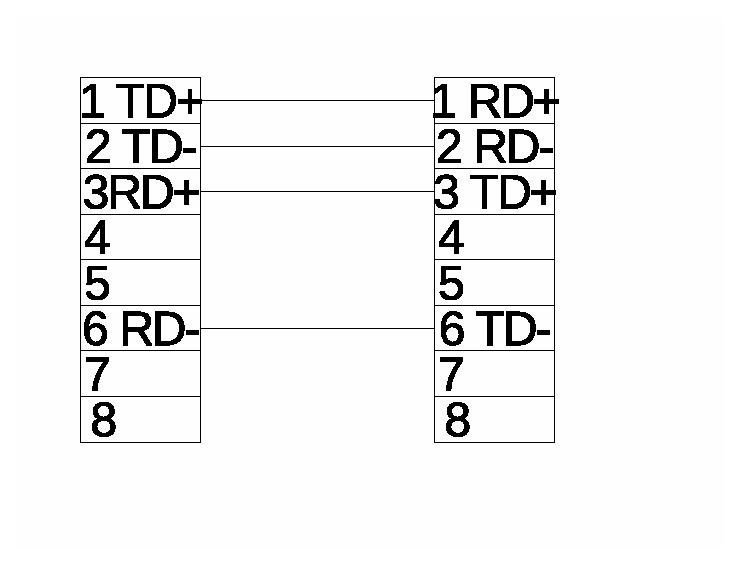
\includegraphics[width=10cm,clip]{draw/cat5pin.eps}
	\caption{10BaseT、100BaseTXのピンアサイン}
	\label{fig:pinassign}
\end{figure}

10BaseT出用いられるCat.3のケーブル、100BaseTXで用いられるCat.5のケーブルでは、各ピンは表\ref{pinassign}のように用いられる。使用されていないピンの間は、配線を省略してある場合がある。図で、TDは送信データ、RDは受信データのためのピンであることを表す。

ツイストペアは、1バント2番、3番と4番、というように、番号が続いているピンにわりあてていく。
Cat.3とCat.5のLANケーブルは、通常、両端のコネクタのピンの、同じ番号同士を結線する。そのため、コネクタに対してこのような結線を行ったケーブルを、ストレートケーブルと呼ぶ。

だが、LANケーブルを使用してネットワークを構成するには、送信側コネクタのTD(送信データ)端子から送信される信号を、受信側ではRD(受信データ)端子で受け取る必要がある。これを、両端の送信と受信の端子を互い違いに接続することから、信号交差と呼ぶ。

だが、HUBとホストの接続ではストレートケーブルを使う。これはなぜであろうか。それは、HUB側のコネクタで、1番と2番ピンに来た信号を受信し、3番と4番から送信する、「信号交差」を行っているからである。つまり、ネットワーク接続するホストの側と、HUBの側では、TDとRDの配置がそっくり入れ替えられている。

では、ホストとホストを直結したり、HUBとHUBを直結したりするというように、ピン配置が同じ機器を接続することはできるのだろうか。そのときは、両端のコネクタの TDのピンとRDのピンを結ぶように結線した、信号交差用のLANケーブルを使用する。
信号交差を行うよう配線したケーブルが、図\ref{fig:cross}のクロスケーブルである。

\begin{figure}[htbp]
	\includegraphics[width=10cm,clip]{draw/cat5cross.eps}
	\caption{クロスケーブル}
	\label{fig:cross}
\end{figure}


最近のHUBのほとんどは、全てのポートで信号交差が必要かどうかを自動判別する機能がある。そのため、ストレートケーブルかクロスケーブルか、つなぐものはホストかHUBかを気にせず使える場合が多い。だが、務用のネットワーク機器には、信号交差が必要か、自動判別を行わないものがある。そのような機器は、ディップスイッチや設定ファイルによって、特定のポートの信号交差を設定する。

\subsection{Cat5eとCat6のピンアサイン}
Cat5eとCat6は、4対8線のケーブルを全て使用する。そのため、図\ref{fig:cat5e}のように、全てのピンを同じ番号のピン同士を配線する。

\begin{figure}[htbp]
	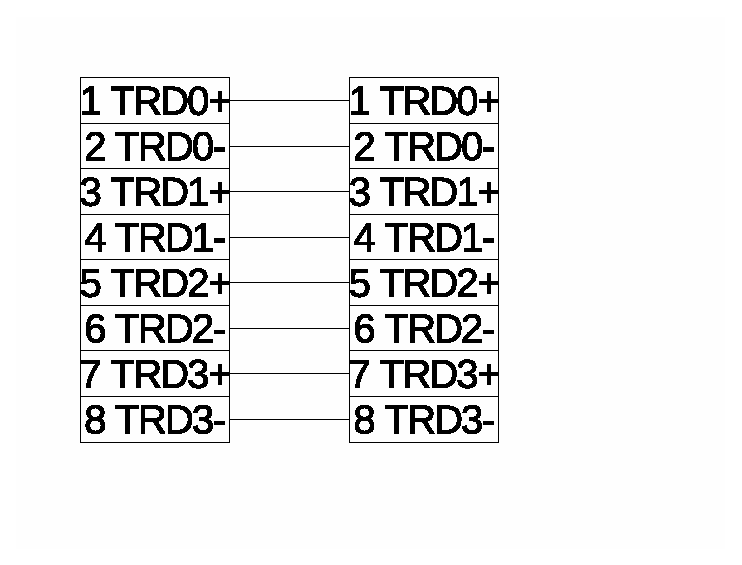
\includegraphics[width=10cm,clip]{draw/cat5e.eps}
	\caption{Cat.5e、Cat.6ケーブル}
	\label{fig:cat5e}
\end{figure}

Cat.5eとCat.6の違いは、イソレータというパーツの有無である。Cat.6は、4対のツイストペアを隔離するイソレータが入っている。

\subsection{カスケード接続}

HUB同士をLANケーブルで接続することを、カスケード接続という。カスケードとは「滝」であり、何段にもなっている滝のようにHUBが接続されている状況を表したものである。では、リピータHUBとスイッチングHUBのそれぞれについて、カスケード接続の説明を行うとどうなるかを説明しよう。

\subsubsection{リピータHUB同士のカスケード接続}

リピータHUB同士をLANケーブルで接続すると、その二つのHUBで構成されるネットワークは、同じ衝突ドメインとなる。リピータHUB同士のカスケード接続は、動作が保証されるのは、信号の速度10Mbpsの10BaseTで4段、100Mbpsの100BaseTXで2段までとされる。

HUBの段数が増えることが、衝突ドメインを構成するネットワークの総延長が延びることと等価であるためである。そのため、カスケード接続の段数は、論理的なケーブルの総延長をを規格内に納めるといういみで制限をされる。

\subsubsection{スイッチングHUB同士のカスケード接続}

次に、スイッチングHUB同士の接続について説明する。これは、同軸ケーブルのときのブリッジが発展したものと考えればよい。つまり、接続されたスイッチングHUBのそれぞれは、同じネットワークであるが、異なる衝突ドメインである。では、ふたつのスイッチングHUBを接続すると、通信はどのように行われるのであろうか。

ここでは、二つのスイッチングHUBのそれぞれを、AとB、と仮称し、そのAとBをカスケード接続する場合で考えていこう。

まず、Aに接続されたインタフェイスの一つからイーサネットフレームが送信されたとする。その宛先が、Aに接続されているインタフェイスのMACアドレスであれば、そのフレームはAの適切なポートに送信される。\footnote{自分自身への送信は、ローカルループバックインタフェイスでバッファリングされ、信号として送出されずに自分からの通信として処理される。}

では、Bに接続されているインタフェイスのMACアドレスを、Aはどのように学習するのだろうか。

BからAに送信されてくるフレームは、全て「Bに接続されている」ポートからくる。そのため、単に、そのポートに接続されている機器のMACアドレスを複数覚えればよい。Bに接続されているホスト宛のイーサネットフレームであれば、Bに接続されているポートに送信する。Bは、MACアドレスとポートの対比表をひいて、フレームを送信するポートを決定する。

Aで全てのポートに送出する必要があると判断されたフレームは、Bの繋がっているポートにも送信される。\footnote{ブロードキャストアドレス宛だけでなく、マルチキャストや未学習の宛先へのフレームの場合もある。}それを受け取ったBは、「Bの中で全てのポートに送出する必要があるか」を判断して、必要であれば全ポートに送出する。

スイッチングHUB同士のカスケード接続は、同じネットワークではあるが、同じ衝突ドメインにならない。だが、スイッチングHUBのカスケード接続は7段が限度とされる。それはなぜだろうか。

スイッチングHUBは、フレームの宛先を読み取り、どのポートに送出するべきかを判断してから適切なポートに送出する。フレームを受信し始めてからどの時点で送出するかでいくつか方式があるが、フレームを受信し始めてから送出するまでの間に、必ず時間差が生じる。この時間差はLANケーブルの総延長が延びていることと同じ意味を持つ。

この遅延は、カスケードするスイッチングHUBの数だけ蓄積される。そのため、衝突を検出できるカスケードの段数は、7段が限界とされている。l

\subsection{スイッチングHUBのJAM信号送出}

先ほど説明したとおり、スイッチングハブは、ポートに到着したフレームをある適度読み込み、宛先のMACアドレスを解釈して、適切なポートに送信する。だが、このメモリの容量は有限である。もし、スイッチングHUBがストア可能なメモリを使いきったら、いったん全ての受信動作を止め、メモリ上のデータを送出する。

また、MACアドレスの学習の結果や、全ポートへの送出で送信したいポートが分かっている状態で、そのポートが別のフレームを送信しようとしている場合もある。

このような場合は、何らかの方法で、その通信に関係するインタフェイスからの通信を止める必要がある。そのための方法として、スイッチングHUBは、擬似的に衝突を発生させる。スイッチングHUBは、CSMA/CDで、衝突による送信の中断を知らせるJAM信号を送出するスイッチングHUBからのJAM信号を受信したインタフェイスは、CSMA/CDに従って、ランダムな時間フレームを送信せずに待つ。

\section{イーサネットとネットワークのループ}

イーサネットは、無線ネットワークのALOHAに由来する。そのため、伝送媒体に送出したフレームが送信者に戻ってくることはない。つまり、伝送媒体にループがあってはならないことはここまでで説明していた。だが、イーサネットでループを作ると、どのような現象が発生するのだろうか。それについて説明を行おう。


\subsection{リピータによるループ}


\begin{figure}[htbp]
	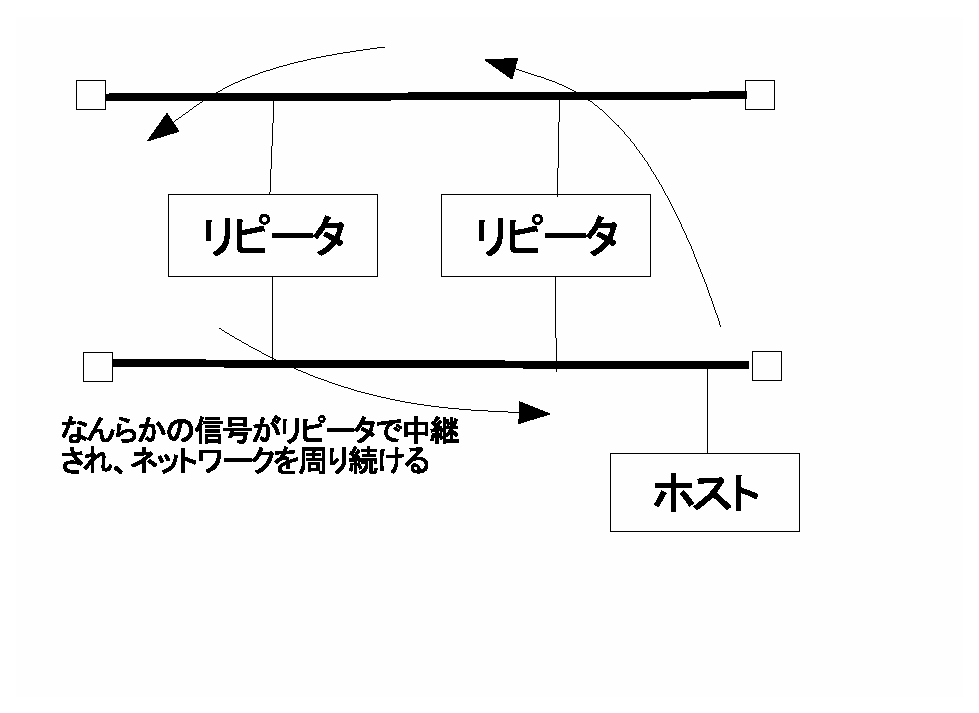
\includegraphics[width=10cm,clip]{draw/repeaterloop.eps}
	\caption{リピータによるループ}
	\label{fig:repeaterloop}
\end{figure}

最初に、イーサネットのループをリピータで作った場合について考えてみよう。たとえば、リピータの両端を同じ同軸ケーブルに接続したり、リピータHUBに接続したLANケーブルを、同じリピータHUBの別の口に接続したような場合である。

繰り返すが、リピータ(リピータHUB)で接続されたネットワークは、CSMA/CDで共有伝送媒体を管理するネットワークであり、同一の衝突ドメインである。

そのどこかでフレームが送信されたとしたら、リピータはそれを中継する。そうすると、ループの中でフレームが周りつつける現象がはっせいする。そうなると、その衝突ドメインに接続されているホストは全て、CSMA/CDに従い、信号がなくなるのを待ち続ける。

その結果、その衝突ドメイン内でのフレームの送信ができなくなる。これが、リピータでループを作ったときに発生する現象である。

\subsection{ブリッジによるループ}

では、ブリッジでループを作るとどうなるか。独立した衝突ドメインが二つ、ブリッジによってリング状に接続されている状況を想定してみよう。

ブリッジでループを作ると、イーサネットフレームが同じネットワークの中を回り続ける現象が発生する。この現象は、ブロードキャストストームと呼ばれる。では、ブロードキャストフレームはどのように生ずるのだろうか。

まず、二つの衝突ドメインを、二つのブリッジで並列に接続した場合を考える。この場合、二つのブリッジが、イーサネットでブロードキャストするフレームを転送し続ける「転送ループ」が生じる。

それぞれの衝突ドメインを、A、Bとして例を示そう。衝突ドメインAで送信されたフレームは、時間差はあっても二つのブリッジに到着する。2台のブリッジの学習が十分でない、もしくはブロードキャストアドレス宛の送信であったなどの理由で、フレームは衝突ドメインBに投げられる。

そのフレームは衝突ドメインB内でブロードキャストされているので、それぞれもう一方のブリッジで受信される。そのブリッジが、衝突ドメインA側のMACアドレスの学習が十分でない、フレームの宛先がブロードキャストアドレスであった、などの理由で、フレームが衝突ドメインAに向けて送信される。

ブリッジはMACアドレスが「どの衝突ドメインから来たか」学習するので、同一のフレームが回り続けると、二つの衝突ドメインの双方に、そのフレームの送信元MACアドレスのホストが存在する、という誤った学習がされてしまう。それによって、MACアドレスの学習テーブルが異常となり、最終的に、ブリッジを越える通信ができなくなる。この現象を、ブリッジのMACアドレスのテーブルが、誤った情報で汚染されることから、MACポイズニングという。

また、同一のフレームが再送信され続けるので、ループ内の通信トラフィックが徐々に増加していく。ブリッジは電気信号の正帰還による発振は発生しない。だが、中継処理の過負荷で故障する可能性がある。

\begin{figure}[htbp]
	\includegraphics[width=12cm,clip]{draw/bridgeloop.eps}
	\caption{誤学習とブロードキャストストームの発生}
	\label{fig:bridgeloop}
\end{figure}


\subsection{スイッチングHUBによるループ}

衝突ドメインがポート毎に独立しているスイッチングHUBでネットワークのループを作ると何が起こるのであろうか。たとえば、一本のLANケーブルの両端を、同じスイッチングHUBの別のポートに接続した場合を考えてみよう。。

この場合、そのスイッチングHUB2接続されたホストから、ブロードキャストフレームなどの、全てのポート宛に送信されるフレームが送信されたとき、問題が発生する。そのフレームがループ接続されているポートに向けて送信されたとき、ループを通って再度別のポートから同じフレームが「送信されてくる。

そうすると、このフレームを再度全ポートに向けて送信し直す転送ループが発生し、通信量が増加していく。もしこのスイッチングHUBが別のHUBに接続されているとすれば、そのHUBへも拡大再生産されるトラフィックをばらまくことになる。この現象を、ブロードキャストストームと呼んでいる。

また、ループによって、先だって説明したMACポイズニングが発生し、正しいポートへの転送ができなくなる、という問題も生じる。

\subsection{イーサネットのループと冗長化}
たった一カ所のループで同じネットワークの通信が実質的に不可能になるのが、イーサネットの最大の弱点である。

イーサネットでは、ネットワーク上にループを作ってはならない。繰り返すが、イーサネットがイーサネットであることに由来する、唯一最大の弱点である。またこれは、イーサネットは、そのままでは複数の経路による冗長化ができない、ということでもある。

逆に言えば、イーサネットにおいて、ループができたとき自動的にそれを回避することと、複数の経路による冗長化を実現することは、同じ意味を持つわけだ。

ループの回避と冗長化を実現する方法として、802.1Dスパニングツリーアルゴリズムという規格が存在する。本書では、スパニングツリーについては、詳細には立ち入らない。そんな方法があるとだけ覚えておいてもらい、普段はループを作らないことに気をつけてもらいたい。

\section{イーサネットの規格}

ここまでで紹介したものでも、イーサネットには、伝送媒体に同軸ケーブルを使用するもの、HUBとLANケーブルを使用するものがあった。実際、これまでの説明では、同軸ケーブルを使う、LANケーブルとHUBを使う、など、主に伝送媒体の種類でイーサネットの規格を区別してきた。

今度はそれを、イーサネットの規格名で表してみることにしよう。イーサーネットの規格は、Mbps単位の通信速度、フレームのビット列の変調方式、通信媒体の種類もしくはネットワークの1セグメント最大長\footnote{同軸ケーブルを使用する規格では、100を単位として表す。それ以外のケーブルを使う規格では、ケーブル長は規格名称に用いない。}というルールになっている。

歴史的経緯のあるものも含め、使用されることの多い規格をいくつか紹介する。ここでは省略したが、イーサネットには、光ファイバを伝送媒体として使用する規格もある。光ファイバの利点は、一般にセグメント距離が同じ速度の規格で使用する電気ケーブル\footnote{通信の分野では、金属線、銅線という意味で「メタル」「カッパー」という用語を用いる}よりも長くすることができる点である。たとえば、ビルのバックボーン\footnote{上下のフロアを貫く、縦方向の共用導管}を経由する接続など、 100メートル以上ケーブルを敷設しなければならない場合などに使用される。

\begin{table}[htbp]  \label{ethernet}
\begin{center}
\begin{tabularx}{110mm}{XXXXXX} \toprule
規格名 & 俗称 & 通信速度 & ケーブル & セグメント距離 & 全二重\\ \midrule
10Base2 & Thin Eternet & 10Mbps & 50Ωシン同軸ケーブル(5mm) & 185m & なし \\
10Base5 & Thick Ethernet & 10Mbps & 50Ωシック同軸ケーブル(12mm) & 500m & なし \\
10BaseT &- & 10Mbps & UTP/STP Cat.3,4,5 & 100m & あり\\
10Broad36 & - &10Mbps & 75Ω同軸ケーブル & 3600m & なし\\
100BaseTX & Fast Ethernet & 100Mbps & UTP Cat.5 & 100m & あり\\
1000BaseT &Gigabit Ether GbE & 1000Mbps & UTP Cat5e & 100m & あり\\
10GBaseT & - & 10Gbps & UTP Cat6 & 100m & 必須\\ \bottomrule
\end{tabularx}
\end{center} \caption{イーサネットの規格}
\end{table}

\begin{figure}[htbp]
	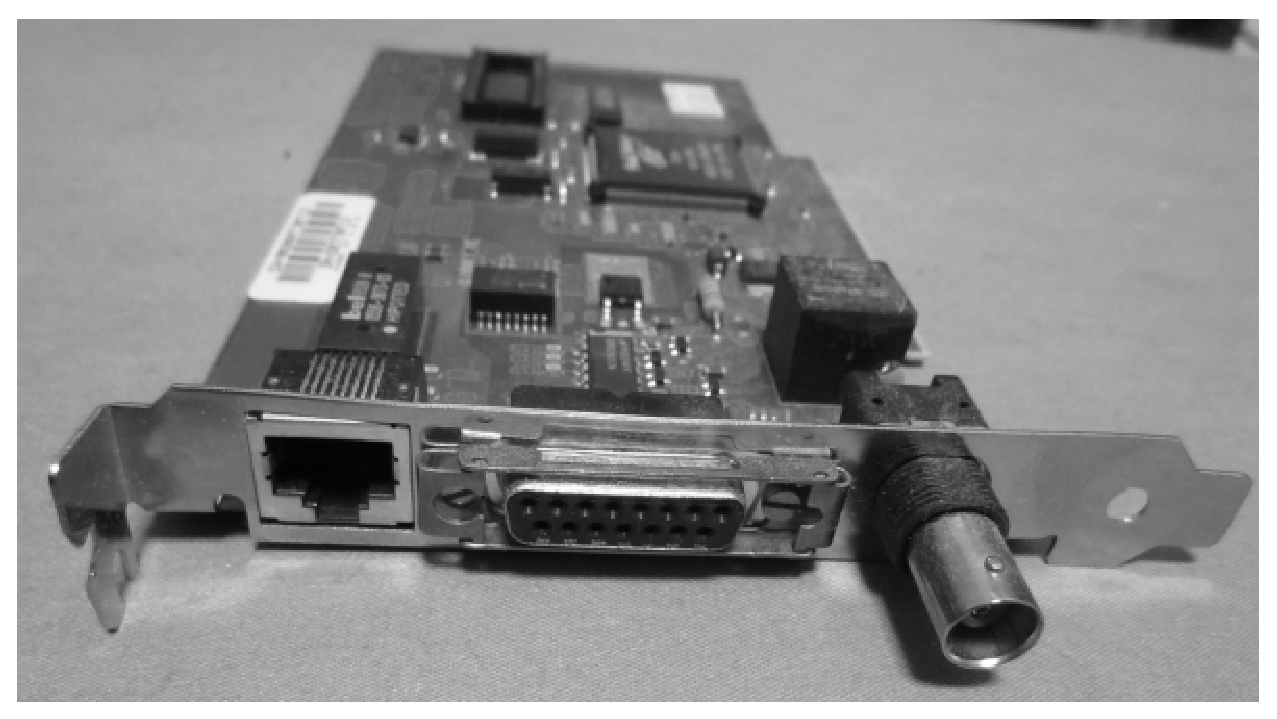
\includegraphics[width=12cm,clip]{draw/3com.eps}
	\caption{3Com EtherLink III PCI}
	\label{fig:3com}
\end{figure}

図\ref{fig:3com}は、左から10BaseT、10Base5(AUI)、10Base2の、三つのイーサネット規格のインタフェイスを搭載したネットワークカード、3ComのEtherLink III PCIである。

\subsection*{}
\begin{itembox}[l]{いもうとコラム 1000BaseTX}
ギガビットイーサネットの規格名は、1000BaseTです。1000BaseTは、4対のツイストペア全てを使って通信します。それぞれのツイストペアを、通信の上り下りで共用し、250Mbpsの速度で通信を行います。それによって、トータルで、全二重1Gbpsの速度を出しています。

ですが、4対のツイストペアのそれぞれを上り下りで共用する、ということは、ツイストペアごとの送受信回路と、送受信の信号を分離する回路とが必要になります。これはGbE製品が出始めた頃は、ネットワーク機器のコストを押し上げる一因と考えられていました。

そこで提案されたのがもう一つのGbE規格、1000BaseTXです。1000BaseTXは、ネットワーク機器を構成する部品を減ら氏、コストダウンすることを目的として、提案されました。

1000BaseTXは、4対のツイストペアを、2対づつ、上り専用、下り専用で使い分けます。そして、各ツイストペアで500Mbpsの速度で通信を行い、全体で全二重1Gbpsの速度を出します。
そして、ツイストペアごとに500Mbpsの通信を可能とするLANケーブルとして、イソレータ入りケーブルのCat.6の規格が定められました。

理屈の上では1000BaseTXは、Cat.6を必要とするケーブルのコストは高いものの、部品点数の少なくなるネットワーク機器のコストは安い、という規格になるはずでした。ですが、1000BaseT対応機器の価格が予想よりも速いペースで下がったことから、1000BaseTXは対抗機器が市販されることなく消えていきました。

いまでは、1000BaseTXは、Cat.6ケーブルにその名残を残すだけです。Cat.6ケーブルは、1000BaseTでも使用できるもの、電気信号レベルでは非互換で、相互接続性がありません。そのため、機器が販売されていたら、1000BaseTと相互接続できないことに起因する問題を起こしていたでしょう。


\end{itembox}


\section{ベースバンドとブロードバンド}

イーサネット規格の名称には、BASEとBROADの二種類があった、これは何を表すものでであろうか。

まず、規格上は10BROAD36に名を残すのみであるBROADについて説明しよう。BROADは、広帯域変調(ブロードバンド変調)であり、WANの速度が速いという意味で誤用されているブロードバンドとではない。では、変調とはなにか。変調とは、伝送したい信号よりも、伝送媒体での伝播特性がよい周波数の信号に、伝送したい信号をのせて送り出すことである。この、伝送特性が良い周波数の信号を、搬送波(キャリア)という。

ラジオのAMやFMというのも、それぞれ、振幅変調(Amplifire Modulation)、周波数変調(Frequency Moduulation)、という変調方式の名称からきている。

一方のBASEとはベースバンド方式という伝送方法になる。ベースバンド方式は、伝送したい信号を変調せずにそのまま伝送媒体に流す。例えば、アナログ電話は変調を行わないのでベースバンド伝送である。また、ステレオミニプラグからヘッドフォンまでのオーディオケーブルに流れる信号も、出力する音声そのものなので、ベースバンドで伝送している信号である。

イーサネットの規格のほとんどは、フレームのビット列から伝相場いたで送信しやすい波形を作った上で、それを変調せずにそのまま電気信号として流す、ベースバンド方式を用いている。

イーサネットでブロードバンド変調を行うのは、CATV向けの同軸ケーブルに、テレビ電波と一緒に信号を送信する規格である10BROAD36のみである。\footnote{余談ながら、フレッツTVという形で、インターネット接続、電話線、ケーブルテレビの重畳を行う通信が復活していることは興味深い}

\subsection{ベースバンドと符号化}

ベースバンド方式を用いるイーサネットの規格では、ビット列の1と0でそのまま信号をオンオフしているのではないかと、ここまでの説明で考えたかもしれない。ベースバンド方式では、ビット列を何らかの形で時系列方向の電圧の変化に置き換える必要がある。この置き換えを、符号化と呼んでいる。

一番簡単な方法として、先に挙げたように、1のときだけ信号を流して0の時は信号を流さない、というやり方が考えられる。だが、この方法は実用的ではない。なぜなら、送受信の双方で、何らかの方法で、タイミングの同期を図る必要がある。そうでなければ、1や0が連続したとき、いくつ1や0が続いていたのかが分からない。だが、イーサネットでは、複数のノードが同期した時計を共有する、という仕組みは持っていない。

次に、1を電圧のH、0を電圧のLとする2値符号方式が考えられるだろう。だが、これも、送受信する双方でクロックの同期が必要となる。なぜなら、これも同じ値が続けば、同じ値のビットが連続したときに、いくつそれが続いていたのかわからなくなる。

では、実際にはどのような符号化の方法が採られているのであろうか。ここでは10BaseTで使用されるマンチェスター符号と100BaseTXで使用される4B5B+MLT-3についてごく簡単に説明しよう。

\subsubsection{マンチェスター符号化}
マンチェスター符号は、電圧がHからLに変化する場合は0、LからHに変化する場合を1として扱う符号化方式である。1でも0でも、1ビットの信号のうちにかならず電圧の変化が生じる。送信側と受信側での信号の同期には、その電圧変化をクロックとして用いることができる。

マンチェスター符号化の欠点は、信号の電圧変化が大きいことである。では、これがなぜ欠点になるのであろうか。マンチェスター符号をフーリエ変換して周波数成分をもとめると、それを構成する周波数の成分が多い。つまり、周波数の幅が広い。\footnote{この周波数の幅を、側波帯という。}。これは、影響を受けるノイズの周波数が多いということであり、ノイズに弱いということである。そのため、マンチェスター符号は、100Mbpsのイーサネットでは使用することができない。

\begin{figure}[htbp]
	\includegraphics[width=12cm,clip]{draw/manchester.eps}
	\caption{マンチェスター符号と4B5B+MLT3}
	\label{fig:manchester}
\end{figure}

\subsubsection{4B5B+MLT5}
では、100BaseTXで使用される4B5B+MLT-3という符号化はどういうものか説明しよう。マンチェスター符号が、構成する周波数成分が多くて100Mbpsで使用できないということであったので、周波数成分が狭いのではないかという予想がつく。たしかに、4B5B+MLT-3は、マンチェスター符号化より周波数成分が狭い。

4B5B+MLT-3とは、連続する4ビットを5ビットに変換する、4B5Bマッピングと、MLT-3という符号化方式を組み合わせた符号化方式である。

MLT-3とは、三値の状態を持つ。そして、1で電圧が上下に一つ変化、0は変化なしという符号化である。この方式は電圧変化がマンチェスター符号よりゆるやかであるため、フーリエ変換した際に、構成する周波数が少ない。つまり、影響を受けるノイズの周波数が少ないということであり、比較的ノイズに強い。

だが、この符号化方式では、0が連続すると同期がとれなくなる。そのため、4ビットを5ビットにマッピングし、連続する5ビットのうち1が二つ以上入るようにする。これが、4B5Bという名称の理由である。\footnote{4B5Bは、変換表で変換する。変換表については本書では割愛するが、必要であれば電気通信の教科書などを参照して欲しい。}

100BaseTXでは、この二つの符号化方式を併用する。そのため、符号化方式の名称が4B5B+MLT-3となる。

\subsubsection{ギガビットイーサネットの符号化方式}
ギガビットイーサネットでは、8B1Q4+4D-PAMという符号化方式を用いる。8B1Qは、8ビットをエラー訂正ビットを加えた9ビットにマッピングし、5進数(Quinary)4桁であらわす。

8B1Qは、エラー訂正ビットを含めた9bitの先頭3bitから、残り6bitの変換表を決定し、5進数4桁に変換する。実際に、9bitは0から511まで、5進数4桁は0から624まで表現することができるので、9bitをマッピングすることが可能である。

4D-PAM5では、その4桁の5進数の核桁を、LANケーブルの4組あるツイストペアに対応させる。それによって、全てのツイストペアを使って、8bitを一度に送出する。

\subsection*{}
\begin{itembox}[l]{いもうとコラム 無線通信のベースバンド方式}
ここまで、イーサネットで用いる、有線通信でのベースバンド方式について見てきました。では、、無線通信におけるベースバンド方式とはどのようなものなのでしょうか。

無線で、ベースバンド方式の送信機は、マルコーニが実用化した火花送信機と、その改良型しか存在しません。火花送信機とは、スイッチのオンオフによる電流のオンオフを、そのままコイルで誘導電流のオンオフとします。そのコイルは放電電極に接続されています。そして、放電電極からの火花放電による電磁波をアンテナから放出するという仕組みです。

火花送信機から発射される電波はホワイトノイズです。つまり帯域幅がものすごく広いため、現在のように細かく周波数を区切ってその用途を指定する電波の使い方をする際の障害となってしまいます。なので、、1955年以降は、国際電気通信条約付属無線規則で使用が禁止されました。

日本に現存する火花送信機は、三六式無線機です。これは戦艦三笠に搭載されていました。実物は東京都墨田区の郵政博物館に収蔵されています。また、横須賀の記念艦三笠では、三六式無線機のレプリカが展示されています。

最後に余談ながら、誤解されていることも多いですが、現代の、モールス信号による無線通信のための送信機は、搬送波にキーのオンオフを印加した変調波で通信を行っています。
\end{itembox}


\section{イーサネットフレーム}

ここまで、ネットワークアクセス層にイーサネットを使用した場合の送出単位、という意味で、イーサネットフレームという用語を使用してきた。では、イーサネットフレームの構造について説明しよう。。

イーサネットフレームは、イーサネットに送出されるデータの単位である。イーサネットフレームの長さは、64オクテットから1518オクテットまでの可変長となる。ここで、オクテット(octet)という表現を用いたが、意味はbyteとおなじ、8bitを単位としたデータ量である。\footnote{デー通信では、9ビットの単位として、byteでなく、octetを用いることがある。ネットワークアクセス層以下では、オクテットと呼ばれることが多い。}

イーサネットフレームの構造は、図\ref{fig:etherframe}のように表すことができる。。

\begin{figure}[htbp]
	\includegraphics[width=14cm,clip]{draw/ethernetframe.eps}
	\caption{イーサネットフレーム}
	\label{fig:etherframe}
\end{figure}


\begin{description}
\item[プリアンプル]信号を共有チャネルを使用するデバイスが認識する時間をとるためのリード。最近のコンスタントシグナリングを使用する規格では実質的に使用しないが、フレーム構造の維持のためにつけられる
\item[宛先アドレス]データの宛先ネットワークインタフェイスのMACアドレス
\item[発信元アドレス]データの発信元ネットワークインタフェイスのMACアドレス
\item[タイプ/長さ]1500より小さい数のときはデータのオクテット長。1536より大きい数のときは上位プロトコルの種類を表すフィールドとなる。
\item[データ]46octet~1500octetの可変長。イーサネットフレームに乗せるデータを1500octet以内の大きさにするのは上位プロトコルの役目
\item[フレームチェックシーケンス(FCS)]CRCによって、プリアンプルを除くフィールドの値にエラーが生じていないかをチェックする。文献によっては、FCSではなくCRCと記載していることがある。
\end{description}

イーサネットフレームの最小の大きさは64オクテット(512bit)となる。これは、10Base5における線路長の最大が2500メートル\footnote{500メートルの同軸ケーブルからなるセグメント3本を、500メートル長の渡り線をもつリピータ2台で接続してひとつの衝突ドメインとした場合の数字である。}であることから決定された。


受信した情報にエラーが生じている可能性があっても、Ethernetのには再送やそのリクエスト機能はない。単に、該当するフレームを破棄するのみである。あるフレームが破棄された場合に、再送するかどうかを判断するのは、ネットワークアクセス層よりも上位プロトコルの役目である。

\subsection{MTUとフラグメント}

先ほど、イーサネットフレームの最小の大きさが64オクテットであるという説明を行った。では、逆に、フレームの最大の大きさというのはどのように決定されるのであろうか. 

二章に分けて行ったネットワークアクセス層に関する話題の最後に、フレームの大きさを決定するMTUと、MTUに起因するフラグメントについて簡単に説明を行なおう。

ネットワークアクセス層のフレームにおける、データ部分の最大の大きさを、MTU(Maximum Transmission Unit 最大転送単位)という。MTUは、イーサネットに限らず、全てのネットワークアクセス層に存在する概念である。たとえば、イーサネットやPPPのMTUは 1500でとなる。

例外がSLIPで、これはIPデータグラムをそのまま流すものであるため、ネットワークアクセス層としてのMTUの概念がない。\footnote{後ほど改めて説明するが、IPv4の場合、IPデータグラムの最大のサイズである64Kbyteが、その最大サイズであると言うこともできる。}

MTUとは、そのネットワークアクセス層で、一度の送信によって運ぶことができるデータ量の上限である。つまり、送信するデータが、通信に使用するネットワークアクセス層のMTUより大きい場合には、データのサイズをMTUよりも小さくなるように分割し、受信側ではその切片を集めて元のデータを取り出さなければならない。これがフラグメントである。

\subsubsection{フラグメント}
ネットワークアクセス層には、データを分割(フラグメント)したり、フラグメントされたデータを元に戻したりする機能がない。データを元に戻せるように分割(フラグメント)し、フラグメントを集めて元に戻すことを担当するのは、上位層である。

フラグメントを担当する層は、IPv4とIPv6で異なる。
IPv4でフラグメントを担当するのは、インターネットプロトコル層である。トランスポート層にはパスMTUディスカバリという機能があり、経路のMTUを検出することが可能である。そして、基本機能としてフラグメントが実装されているのはインターネットプロトコル層となる。

\subsubsection{最小MTU}
上位層にIPv6を使用する場合、最小MTUというものが規定されている。最小の「最大転送単位」というのも変なものだが、上位プロトコルの都合で、MTUとして最低限確保しなければならないデータサイズのことである。

上位にIPv6を使用する場合は、1280byteが最小となる。IPv4には明確な規定はないが、あえていうならヘッダ長20byteにデータ長をくわえた長さになる。

\subsection{タイプ・長さフィールド}
イーサネットフレームの中には、タイプ・長さというフィールドがある。十進数で1500以下ならオクテット長としてのサイズ、1536以上ならデータ部分がどのプロトコルのデータであるかを洗わすタイプとなる。
この違いは、かつてDIX\footnote{DEC,Intel,Xerox}仕様とも呼ばれた初期のイーサネットと、DIX仕様を基としてIEEEで規格化された802.3との相違によって生じたものである。

DIX仕様では、このフィールドは、フレームがどの上位プロトコルのデータをカプセル化しているかを表すものである。たとえば、IPv4IPアドレスを持つデータグラムであれば、十六進数で0800(十進数で2048)を入れる。これで判るように、DIX仕様の時は、イーサネットのフレームにはデータ長を表すフィールドがなかった。

一方、IEEE802.3では、このフィールドはデータ部分のオクテット長でのサイズとなる。では、逆にデータのタイプフィールドはどこに行ったのだろうか。802.3規格では、データ部分の先頭に、タイプなどの付加情報を付加するというものであった。

DIX仕様のフレームと802.3のフレームは、このフィールドを見ることで区別することができる。実際の機器は、この二つの形式のフレームをどちらも同様に取り扱うことが可能である。

もっとも、現在は、上位層はインターネットプロトコルでほぼ決め打ちすることができる。そのため、このフィールドは長さとして使う802.3方式だが、データのタイプを表すヘッダを省略したDIX仕様方式、という折衷的なフレームが用いられることが多い。\footnote{実のところ、これは過去にNovel 802.3Rawと呼ばれた規格と同じ形式である。Novellが802.3ドラフトを基に、イーサネットでIPXのデータを伝送するために定めた規格が後に、このように呼ばれた。上位層のプロトコルをIPXで決め打ちとしたため、データタイプのフィールドが省略された。}



\subsection{ジャンボフレーム}
ギガビットイーサネットでは、接続可能なネットワークの総延長をかせぐために、フレームのサイズを大きくする。つまり、送出する時間を延ばすという方法をとる。

それであれば、イーサネットフレームのペイロードそのものを大きくしてしまっても、同じである。その考えで、ペイロードを大きくしたイーサネットフレームを、ジャンボフレームと呼ぶ。

ジャンボフレームはイーサネットの規格で正式に定められたものではなく、ベンダ規格である。そのため、接続する危機感では、互換性がとれず、ジャンボフレームで通信できないことがある。


\subsection*{}
\begin{itembox}[l]{いもうとコラム PPPoE}
先に説明したPPPは、接続手順、認証機能、切断手順が存在します。これらの機能は、伝送媒体がなにであるかにかかわらず、必要となる場合があります。

接続時認証や、接続・切断をイーサネットの上で制御したいときは、イーサネットの上でPPPを用いることで実現できます。この、イーサネットの上でPPPによる接続を行うこのが、RFC2516で提案されたPPPoE(PPP on Ethernet)です。\footnote{ただし、PPPoEのPPPヘッダは、シリアル(電話線)で使用するPPPとは異なります。PPPoEは、PPPのフレームをそのままイーサネットに乗せているわけではありません。 }

たとえば、NTT東西のインターネット接続サービスであるフレッツADSLやB-Fletsは、プロバイダとの接続のためのプロトコルとして、PPPoEが用いられています。

PPPoEでは、イーサネットフレームの上に、PPPのフレームを押し込んで通信します。当然ながら、PPPoEを用いた場合、PPPoEのフレームの中にインターネットプロトコル層から渡されたフレームを詰め込むので、それによるオーバヘッドが生じます。

\end{itembox}



\chapter{インターネットプロトコル層(その1) インターネットプロトコルの概論}

この章では、インターネットプロトコルスイートにおける、インターネットプロトコル層について、概論的な説明をします。インターネットプロトコル層は、トランスポート層にどのようなサービスを提供するのでしょうか。そして、どのようにネットワークアクセス層を利用しているのでしょうか。

インターネットプロトコル層とは、その名の通り、複数のネットワークとネットワークの間で通信を行うためのプロトコルです。そして、TCP/IPのIPに相当するプロトコルでもあります。

何らかの機器をインターネット接続する際に、必ず、IPアドレスという言葉がでてきます。このIPとはInternet Protocolであり、略さずに言えば、Internet Protocol Addressとなります。では、インターネットプロトコルとはなにであるのか、そして、IPアドレスとは何であるのかを説明していくことにしましょう。

\section{インターネット}

インターネットとという言葉ある。そして、インターネットプロトコル層というレイヤーがある。

なぜインターネットプロトコル層が必要なのだろうか?ネットワークアクセス層の章を読み進めいていただいていたら、このような疑問を持たれるかもしれない。
そして、ネットワークアクセス層だけで世界中と通信すればいいのに、そうしない理由は何なのだろうか。

前章で説明したように、ネットワークコミュニケーション層の物理的な規格とプロトコルには、いろいろなものがある。イーサネットは狭い範囲でホストの数が多い場合に向いているし、PPPは、距離にかかわらず、一対一接続を行う場合に向いている。

それなら、ネットワークコミュニケーション層ごとに、プロトコル変換を行うものを置けばいいと思うかもしれない。だが、それなら、複数のネットワークを結ぶプロトコルを定めて、ネットワークアクセス層と、ネットワーク間のプロトコルを取り持つ機器にした方が汎用性が増すのではないだろうか。

そのような発想で、インターネットプロトコルが生まれた。インターネットという言葉は、inter-netである。つまり、ネットワークとネットワークの間、ということだ。

\subsection{インターネットプロトコル層の昔話}

ここでも、インターネットプロトコル成立前夜の状況を振り返る昔話から始めよう。規格の由来というのは、全て昔話のなかに隠れている。
後のインターネットに受け継がれる思想と技術は、1960年代後半から、アメリカの四つの大学を結ぶネットワークのARPANETからはじまった。

そんな中、ロバート・カーンは衛星パケット網と地上の無線パケット網の相互接続実験を行っていた。その過程で、カーンは、異なるネットワークの相互接続ができるということについての知見を得た。
今の用語で言えば、異なる構造のネットワークアクセス層同士の通信を行う、ということである。
現在でも、一般的なインターネット接続は、LANとインターネット接続回線という、異なる構造のネットワークアクセス層どうしの通信を行っている。
TCP/IPの原初の形は1973年から1974年頃に、RFC675としてまとめられた。ALTO ALOHAがEthernetという名前になる前後である。このころは、LANを構成するための、ネットワークコミュニケーション層相当の規格でも、ベンダーごとにまちまちな構造、規格、プロトコルであった。

\subsection{異なるネットワークの間の通信}

異なるネットワーク間で通信をするということは、それぞれの機器が直接に接続されているネットワークコミュニケーション層の規格を問わず、エンドツーエンドでデータを届けるということである。
それぞれのネットワークは、自分と、自分以外のネットワーク全てが、そのネットワークコミュニケーション層では、宛先にフレームを届けることができることを期待する。

もうひとつ、あるネットワークから来たパケットからデータを取りだして、宛先となるネットワーク宛のパケットに作り直して送る、中継の仕組みも用意しよう。
この二つで、異なるネットワークの間で、とりあえずデータを相互に送りあうことができるだろう。

では、この異なるネットワークでデータを相互に送りあうこととはどういうことか、二つのネットワークを繋ぐところから初めて、順を追って説明していこう。

\subsection{二つのネットワークを結ぶ}

\begin{figure}[htbp]
	\includegraphics[width=12cm,clip]{draw/ip_basic2.eps}
	\caption{二つのネットワークを結ぶ}
	\label{fig:ip_basic2}
\end{figure}

二つのネットワークを一つの中継役が結んでいる場合で考えてみよう。中継役はネットワークAとネットワークBとに接続されたコンピュータである。そして、それぞれのネットワークに対してネットワークコミュニケーション層のプロトコルで通信することができる。
だが、ネットワークAとおネットワークBhは、ネットワークコミュニケーション層のプロトコルでは相互に通信でないとする。

ネットワークAのホストからネットワークBのホストに宛てた通信は、とりあえず中継役に送る。中継役は、ネットワークB宛の通信が届いたら、ネットワークBのネットワークコミュニケーション層のプロトコルで、宛先に通信を届ける。ネットワークBからネットワークAへの通信も同様である。

中継役を置くことで、それぞれのネットワークに属するホストが、自分の所属していない側のネットワークコミュニケーション層の情報をもっていないくても、相互に通信が可能になる。つまり、自分以外のネットワークに関して、持っていなければならない情報を減らすことができる。

一方、中継役は、中継に必要なアプリケーションのみ動作させればいい。
そのため、コンピュータとしてのリソースを中継に使うことができる。

\subsection{三つ以上のネットワークを結ぶ}

つぎに、三つ以上のネットワークを結ぶ場合を考えてみよう。三つ以上のネットワークをそれぞれ中継役で結んでやる。ここでは、簡単にするために、図\ref{fig:ip_basic3}のようにネットワークが接続されているとしよう。

ネットワークAとネットワークB、ネットワークBとネットワークCの」間の通信は、先に説明したふたつのネットワークを接続した場合となる。では、ネットワークAとネットワークCの間の通信はどうなるのであろうか。

ネットワークAの中のホストは、宛先をネットワークCのホストにした通信を、ネットワークAとネットワークBの中継役に転送する。ネットワークAとネットワークBの中継役は、宛先がCであるのを確認すると、ネットワークB二接続されている、ネットワークBとネットワークCの中継役に転送する。最終的に、ネットワークBとネットワークCの中継役が、ネットワークCに接続されたホストに中継する。


\begin{figure}[htbp]
	\includegraphics[width=12cm,clip]{draw/ip_basic3.eps}
	\caption{三つ以上のネットワークを結ぶ}
	\label{fig:ip_basic3}
\end{figure}

\subsection{もっとたくさんのネットワークが接続されている場合}

今度は、もっとたくさんのネットワークが接続されている場合について考えてみよう。
中継役は、自分が接続されているネットワークには自分で通信を中継する。また、自分が接続されていないネットワークが宛先であり、他のネットワークへの中継役と接続されていれば、その中継役に中継してもらう。

では、世界のどこかには存在するけれど、どこに存在するか知らない宛先と通信したいときはどうするか。中継役は、自分が知らない宛先への中継を丸投げする、別の中継先というのを知っている。
自分が知らない宛先への通信は、この中継先に丸投げする。

一見いい加減に思える方法であるが、インターネットの通信はこれで成り立っている。中継を繰り返すうちに、宛先へ向かう中継役を知っている中継役にいきつき、それを繰り返して、目的の宛先にたどり着くわけだ。いわばバケツリレーである。だが、廻されたバケツは自分の分かる範囲で適切と思われる宛先に渡す、という紳士協定に、すべての中継役は従っている。

\begin{figure}[htbp]
	\includegraphics[width=12cm,clip]{draw/ip_basic4.eps}
	\caption{もっとたくさんのネットワークを結ぶ}
	\label{fig:ip_basic4}
\end{figure}

\subsection{ルータ}
ここまで中継役という名前で説明してきた機器が、現在ルータと呼ばれるものである。ルータは、届いた通信を、同じネットワークに接続されたホストを含む宛先に適切に中継するための機器である。

ネットワーク間の中継専用の機器であるルータは、1990年代半ばにCisco Networksがはじめて発売した。それ以前は、PCやワークステーションにネットワークインタフェイスを複数取り付け、中継専用に使用することが多かった。

\subsection{パケットとデータグラム}

ルータの通信は、ひとかたまりのデータを送り合う形で行われる。このひとかたまりのデータを、パケット、もしくはデータグラムと呼ぶ。パケット(Packet)は小包、データグラム(Datagram)は、データと電報(Telegram)の複合語である。

パケットには宛先が書かれている。ルータは、宛先情報を参照して、どこにパケットを転送するか決定する。

\subsection{デフォルトルートとルーティング}

ここまで、どこにあるかわからない宛先と通信するときに使う中継先となるルータを、デフォルトルートと呼んでいる。デフォルトルートには、同じネットワークに宛先がなく、宛先に接続されているルータがどこにあるかわからない場合に、とりあえず中継してもらうルータである。
あるネットワークのルータは、宛先が自分の接続されたネットワークでないパケットのうち、つぎにどのルータに転送すれば良いかわからないパケットを、自分のデフォルトルートに転送する。

ルータが一つだけ接続されているネットワークでは、そのルータが必ずデフォルトルートとなる。そのネットワークに接続されたホストは、そのルータをデフォルトルートとして設定することで、外部のネットワークとの通信が可能となる。

また、デフォルトルート以外のルータがあるときに、どのネットワークのホストと通信するときはどのルータに中継してもらう、という情報を、ルーティング情報やルーティングテーブルと呼ぶ。また、ルーティング情報に従って中継するルータを選択することを、ルーティングと呼ぶ。デフォルトルートとの通信も、「知らない宛先」に対するルーティング情報に従ったルーティングである。


\subsection{Tier1とフルルート}

\begin{figure}[htbp]
	\includegraphics[width=12cm,clip]{draw/tier1.eps}
	\caption{Tier1プロバイダとプライベートピア}
	\label{fig:tier1}
\end{figure}


インターネットの通信とは、ここまで説明したバケツリレーを世界規模にしたものである。\footnote{CLANNADで、ことみのテディベアのエピソードを見ながら、インターネットプロトコルのパケットと同じだと思ったのは筆者だけではないであろう。}インターネットでは、ネットワーク毎に、デフォルトルートが存在する。
そして、インターネットの全てのネットワークからのパケットが届けられるルータは、全世界で25万ある経路について、次はどこに転送すればいいかを全て記憶している。

この全ての経路を、フルルートと呼ぶ。そして、フルルートを記録しているルータを管理するインターネットサービスプロバイダを、Tier1プロバイダと呼ぶ。
Tier1は、インターネットで一番多くの経路情報が集まる場所であり、宛先のわからないすべてのパケットが一度は送られる。Tier1のプロバイダを経由すれば、インターネットのどこにでもパケットを送ることができる。

\subsection{インターネットの構造}

インターネットの構造において、Iier1は、最上位のプロバイダになる。Tier1のプロバイダに、下位のプロバイダのネットワークが接続され、そのネットワークに、更に下位のプロバイダが接続される。このように、いくつものネットワークを相互に接続して、最終的にエンドユーザのネットワークに至る。
エンドユーザのネットワークは、そのネットワークに接続された下位のネットワークがない。インターネットの末端にあたる。

インターネットの構造は、Tier1によるネットワークを中心として、そのネットワークを相互接続されたネットワークが何重にも取り囲んでいる。その一番外側に、エンドユーザのネットワークが存在する。

\subsection{プライベートピア}

Tier1以外のプロバイダの間で、プライベートピアと呼ばれる経路が設定されていることがある。
これは、Tier1のプロバイダを介さずにその下位のプロバイダ同士でパケットを交換するための、専用線を使用した経路である。

プライベートピアを敷設する理由は、上位プロバイダと野接続料金の削減がある。プロバイダAとプロバイダBのネットワークの間にプライベートピアを設定すれば、この『プロバイダ間の通信はTier1を通す必要が無い。それによって、パケットが上位のに行くための時間を削減できる。
また、上位のプロバイダと野接続料金を削減する効果もある。データ通信の回線は、パケットの転送数で料金が決まる契約となっていることがある。そのため、撚りやすい回線でプライベートピアを構成すれば、その分の回線費用を抑えることができる。



\subsection{ダイナミックルーティング}

あるパケットが宛先に届くときの経路は、毎回同じであるとは限らない。あるパケットと、その次に届いたパケットは、それぞれ全く別の経路を通って届いた可能性がある。

これは、その時点でのネットワークの状況で経路を決める、ダイナミックルーティングを行うルータが経路の途中にあるためである。ダイナミックルーティングは経路に障害が発生していたり、負荷が高かったりするときに、転送する先のルータを変更する。そのため、パケットの経路は、パケットごとに異なる可能性がある。

\subsection{パケットの到着順}
パケットは、一つ一つの経路が異なる可能性がある。そして、経路が違えば送信した順番を崩して宛先に届くこともある。

インターネットプロトコル層は、パケットが送信順に宛先に届くことを保証しない。もしそれが必要なら、トランスポート層やアプリケーション層でそれを担保するのがインターネットプロトコルスイートの考え方である。
インターネットプロトコル層が担当するのは、パケットを宛先により近そうなルータに向けて転送することだけである。


\subsection{なぜ世界はひとつのイーサネットではないのか}

ここまでの説明で、ルータでなくても、世界中イーサネットにしてブリッジで繋げばいいのではないか、そう思う読者諸兄がいるかもしれない。ここで、ルータとブリッジの違いに触れておこう。

ルータは、適切なルーティングを行うことで、いくつものルータを介して接続された「遠隔」かつ「複数」のネットワークうに対して通信を行うことができる。ネットワークコミュニケーション層よりも広い範囲で、ネットワークを越えた相互通信を行うためにインターネットプロトコル層が存在し、そして、そのための機器としてルータが存在するわけだ。
また、異なる規格のネットワークの間でも、パケットを中継することができる。たとえば、離れた二点間の通信に向くPPP接続によるネットワークと、ある範囲に多数のホストがあるときに向く、イーサネットによるネットワークとの間で、パケットによる通信ができる。

ブリッジは直接接続された衝突ドメイン間での、フレームの転送をを可能とするだけである。
また、規格の異なるネットワークコミュニケーション層のプロトコルを変換氏、相互通信を行うことはできない。
ブリッジで接続されたネットワークは、ネットワークコミュニケーション層での同じネットワークとなり、物理的な大きさの限度が存在する。



\subsection{インターネットプロトコルのアイディア}

ここまで説明したことが、大まかなインターネットプロトコルのアイディアである。初期のTCPとIPの機能は分離していなかった。
ネットワーク間でデータを転送する機能をインターネットプロトコルとして分離させたのは、TCPv3とIPv3という、TCP/IPのいわばバージョン3からである。

その後、IPのバージョンが4となる。このIPv4が、現在インターネットで使用されるアドレスと、それによる転送ルールなどの体系として、現在に至るまで30年以上使用されている。
現在は、IPv4と、その後継となるIPバージョン6、つまりIPv6とが併用されている。

\subsection{コネクションレス通信}

先に説明したように、インターネットプロトコル層のデータの単位を、パケットもしくはデータグラムという。宛先情報であるヘッダと、データから構成されているのが、小包や電報とにていることから付けられた名前である。
パケットとは、電話のように、端から端まで物理的に回線を接続するコネクション型の通信と対比しての呼び方である。両端まで接続された回線をデータが流れるときは、「宛先」情報はいらない。なぜなら、送信する側の反対側が必ず宛先であるからだ。

だが、データに宛先情報を付加し、途中で宛先情報を参照して適切な宛先に転送する仕組みがあれば、たとえ送信側から受信側まで一本の経路が繋がっていなくても、そのデータはいつか宛先に辿り着くだろう。これが、、パケットの考え方である。ここまでの説明の言葉を使えば、宛先の書いてあるバケツということになる。
そのため、パケットを使う通信は、コネクション型通信に対比して、コネクションレス通信と呼ぶ。

\section{そもそもインターネットとは何か}

インターネットという言葉とは、インターネットプロトコルで接続されたネットワークのによって構成されるネットワーク事指す。
ここで気をつけるべきは、インターネットプロトコル使用して相互接続される複数のネットワークなのでインターネットと呼ばれる、ということだ。インターネットで使用するプロトコルだから インターネットプロトコルなのでは内。

\subsection{internnetとInternetの違い}

「インターネット」と読む語には、一般名詞としてのinternetと、固有名詞としてのInternetの二つが存在する。この二つの言葉には、それぞれどんな意味があるのであろうか。簡単にではあるが、辞書を引いてみることにしよう。

\begin{description}
\item[internet]単一の論理ネットワークを構築するために、共通のプロトコルで接続された複数の物理ネットワーク
\item[Internet]小文字で始まるinternetが相互接続された世界規模のネットワーク\footnote{定冠詞をつけてthe Netと表記する場合もある。}
\end{description}
アクセス
一般名詞のinternetは、この章で説明するインターネットプロトコルによって相互接続されたネットワークの集合遺体を指す。辞書的な意味に従えば、二つのネットワークコミュニケーション層をインターネットプロトコルで相互接続すれば、それはもうinternetである。

<<<<<<< HEAD
固有名詞のInternetは、ARPAnetと呼ばれる、1969年に、アメリカで4つの大学を接続することから始まったネットワークの相互接続実験に端を発するネットワークである。
ARPAnetは、もともとTcP/IPを使用していなかった。だが、1980年代初頭にARPAnetのプロトコルがTCP/IPに置き換えられている。

\section{インターネットプロトコル層}

ここまで説明したように、複数のネットワークコミュニケーション層を相互接続するためのレイヤーを、インターネットプロトコル層と呼んでいる。
そして、インターネットプロトコルとは、インターネットプロトコル層で用いる通信規約である。
では、ここから、インターネットプロトコルについて、もう少し立ち入って説明していくことにしよう。

インターネットプロトコルには、おおまかに、以下のような役目がある。

\begin{itemize}
\item ネットワークとホストを識別するための、インターネットプロトコルアドレスを定義する 
\item インターネットプロトコル層でのデータの単位であるデータグラムを定義する 
=======
固有名詞のInternetは、ARPAnetと呼ばれる、1969年に、アメリカで4つの大学を接続することから始まったネットワークの相互接続実験に端を発する。通常の教科書であればARPAnetのはじまりからTCP/IPの導入。発展的解消への歴史を説明すべきところであろう。だが、本書では、ARPAnetはTCP/IPに依って構築されたのでなく、1980年代初頭にARPAnetのプロトコルがTCP/IPに置き換えられた、という卵と鶏のどちらが先かの説明に留めておくことにする。\footnote{ARPAnetの歴史に興味があれば、参考文献に挙げた書籍を参照していただきたい。}




\section{インターネットプロトコル層}

ここまで説明したように、複数のネットワークコミュニケーション層、つまり、物理ネットワークを相互接続するための層を、インターネットプロトコル層と呼んでいる。そして、インターネットプロトコルとは、インターネットプロトコル層で用いる通信規約である。では、ここから、インターネットプロトコルについて、もう少し立ち入って説明していくことにしよう。

インターネットプロトコルには、おおまかに、以下のような役目がある。本章では、この役目の一つ一つについて、説明を行っていく。

\begin{itemize}
\item ネットワークとホストを識別するための、インターネットプロトコルアドレスを定義する 
\item インターネットプロトコル層でのデータの単位であるパケットを定義する 
>>>>>>> d851a4c447b4dfd0eab93c99c783a4e3d57db141
\item ネットワークコミュニケーション層とトランスポート層を仲立ちする 
\item ルーティングする
\item パケットにするには大きすぎるデータがきたとき、分割(フラグメント)する
\end{itemize}

\subsection{IPv4と」IPv6}
概論において簡単な説英を行ったが、現在、インターネットプロトコルにはバージョン4とバージョン6という二つのバージョンが存在する。

<<<<<<< HEAD
もともと、インターネットプロトコルスイートで用いられていたインターネットプロトコル層は、バージョン4である。
だが、90年代に、バージョン4では、各ホストやネットワークを一意に区別するのに用いる番号であるIPアドレスが足りなくなることが予想された。
そのため、取り得るIPアドレスの数を増やすことを第一の目的として策定されたのが、インターネットプロトコルのバージョン6(IPv6)である。
IPv6では、アドレス数を増やす以外の拡張、変更も多く行われている。

本書第6版発行現在(2018年秋)はその過渡期であり、IPv4が主に使われている中、IPv6もユーザに意識させないまま普及が進んでいる。
=======
元々インターネットプロトコルスイートで用いられていたインターネットプロトコル層は、バージョン4である。だが、90年代に、バージョン4では、各ホストやネットワークを一意に区別するのに用いる番号、つまりIPアドレスが足りなくなることが予想された。そのため、取り得るIPアドレスの数を増やすことを第一の目的として策定されたのが、インターネットプロトコルのバージョン6である。IPv6では、アドレス数を増やす以外の拡張、変更も多く行われている。

本書第4版発行現在(2016年夏)はその過渡期であり、IPv4が主に使われている中、IPv6がアーリーアダプタから一般に広まりつつある段階である。

>>>>>>> d851a4c447b4dfd0eab93c99c783a4e3d57db141
本書では、インターネットプロトコルのバージョン4をIPv4、バージョン6をIPv6と表記する。

\subsection{デュアルスタック}

<<<<<<< HEAD
IPv4とIPv6が併用されているということは、ふたつの「インターネットプロトコル」が併用されているということである。

インターネットプロトコルスイートにおいて、インターネットプロトコル層の部分におさまるなにかが、二つ存在するということだ。では、この二つはどのような位置関係にあるのだろうか。
=======
IPv4とIPv6が併用されているということは、すなわち、現在、ふたつの「インターネットプロトコル」が併用されているということでもある。

つまり、インターネットプロトコル層の部分におさまるなにかが、二つ存在するということだ。では、この二つはどのような位置関係にあるのだろうか。
>>>>>>> d851a4c447b4dfd0eab93c99c783a4e3d57db141

インターネットプロトコルスイートの菱餅重ねのなかにIPv4とIPv6をいれななおしてみると、図\ref{fig:dualstack}のように、二つのプロトコルが隣り合った位置に配置される。

トランスポート層は、このどちらの「インターネットプロトコル」も使うことができる。また、どちらのインターネットプロトコル層も、同様にトランスポート層にサービスをする。そして、どちらのインターネットプロトコル層も、ネットワークコミュニケーション層からサービスを受ける。

つまり、実際のネットワークでは、IPv4とIPv6を同時に使うことができるということだ。このことを、インターネットプロトコル層のスタックが二つある、という意味で、デュアルスタックとよんでいる。

\subsection{デュアルスタックの優先順}

\begin{figure}[htbp]
	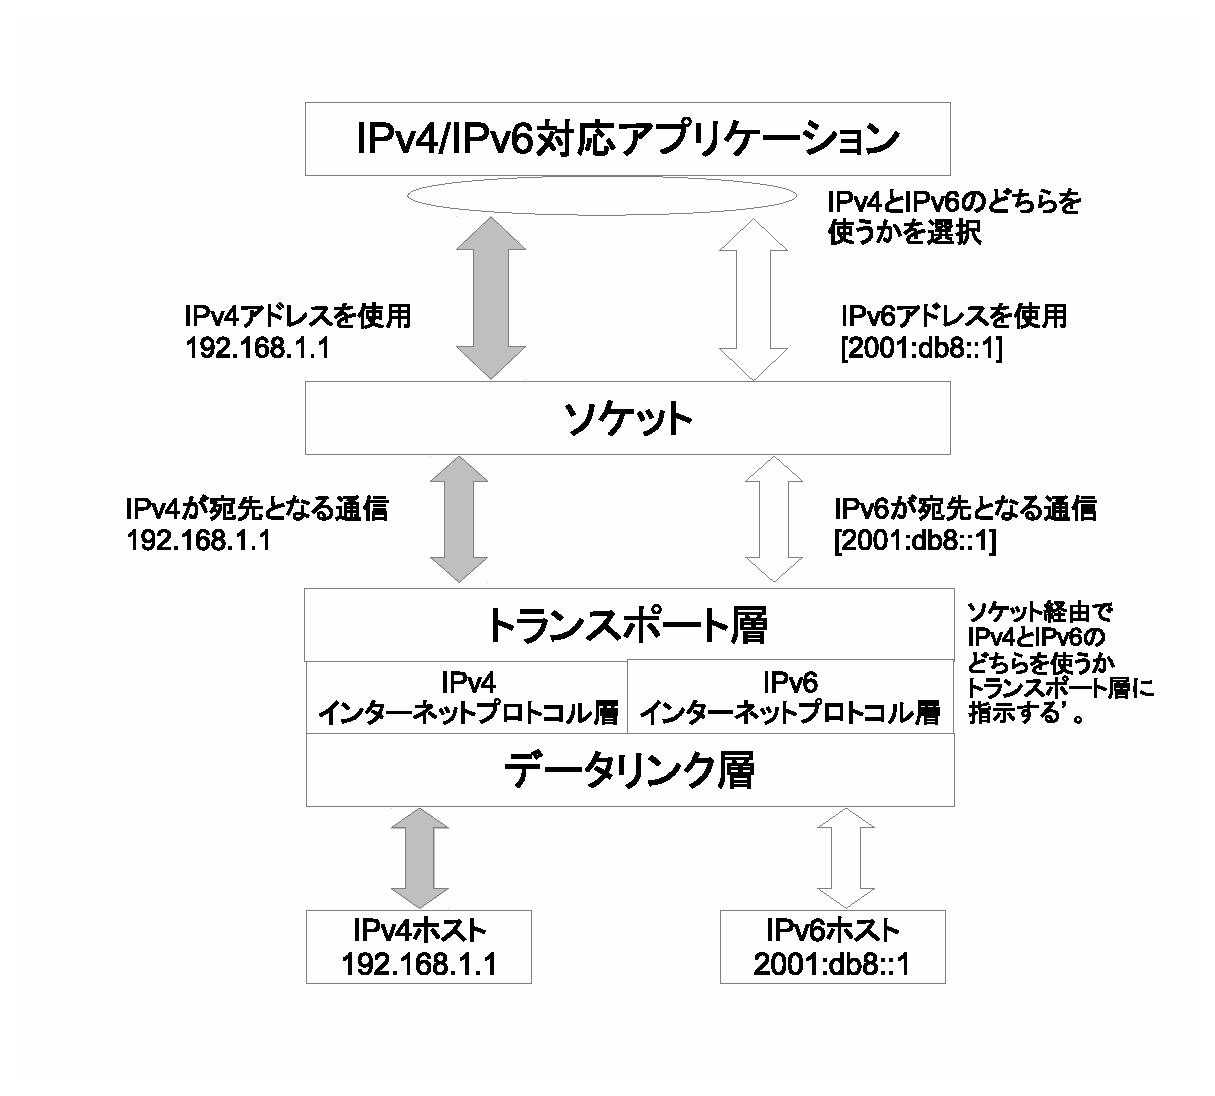
\includegraphics[width=12cm,clip]{draw/doublebind.eps}
	\caption{デュアルスタック}
	\label{fig:dualstack}
\end{figure}

<<<<<<< HEAD
デュアルスタックの環境かつ、IPv4とIPv6のどちらでも、同じホストに到達できる場合、どちらのインターネットプロトコル層を使うのだろうか。
=======
デュアルスタックの環境かつ、IPv4とIPv6のどちらでも、同じホストに到達できる場合を考えてみよう。このとき、どちらのインターネットプロトコル層を使うのだろうか。

>>>>>>> d851a4c447b4dfd0eab93c99c783a4e3d57db141
デュアルスタック環境では、まずIPv6によるアクセスが可能なら、IPv6でのアクセスを試みることになっている。IPv6での接続が規定の時間内に終了しない場合、あらためてIPv4でのアクセスを試みる。

実は、この選択を行うのはアプリケーション層である。実装上、アプリケーションがソケットを開くとき、アドレスファミリを選択することで、IPv4とIPv6のどチラを使うか、どちらから使うかを選択する。
IPv4のスタックはIPv4のスタックとしか通信できない。IPv6も、IPv6としか通信できない。インターネットプロトコル層には、どちらのスタックを使うべきかの判断をする自動判別のロジックは持っていない。


\section{インターネットプロトコルアドレス}

インターネットプロトコルという言葉で最初に思いつくものはなにであろうか。それはおそらく、インターネットプロトコルアドレス(Internet Protocol Address、以降IPアドレス)ではないだろうか。

IPアドレスとはその名の通り、インターネットプロトコルで接続されるネットワークにおいて、ホストとネットワークを識別するためにユニークにつけられる番号であり、これをアドレス\footnote{後で説明するように数字の列であるが、建物の号室表示までついた文字通りの住所と考えてよい。}と呼び表す。

\subsection{IPv4アドレスとIPv6アドレス}

<<<<<<< HEAD
先だって、インターネットプロトコル層として、二つのバージョンが併用されているという話をした。つまりIPアドレスも、それぞれのバージョンに対応したものが存在する。

IPアドレスは、最初は、IPv4の形式が実用化された。4組の数字をドットで区切った、192.168.1.1というような形式のアドレスである。
このIPv4でのIPアドレスは、32bitのビット列によって表される。数字表記は、人間が理解しやすいようにするために、先頭から8bitごとに区切って、それを十進数であらわしたものとなる。

IPv4アドレスは、0.0.0.0から255.255.255.255までのアドレスを取り得る。
では、IPv4アドレスはいくつ存在すのだろうか。IPv4アドレスは、32bit長なので、$2^{32}$個存在することができる。これを書き下すと4294967296個で、約43億個である。
=======
先だって、インターネットプロトコル層として、二つのバージョンが併用されているという話をした。ということは、IPアドレスも、それぞれのバージョンに対応したものがあるということであろうか、そう考える読者諸兄もいるであろう。その予想は正しい。

IPアドレスは、最初は、IPv4の形式が実用化された。4組の数字をドットで区切った、192.168.1.1というような形式のアドレスである。
このIPv4でのIPアドレスは、32bitのビット列によって表される。数字表記は、人間が理解しやすいようにするために、先頭から8bitごとに区切って、それを十進数であらわしたものとなる。

つまり、IPv4アドレスは、0.0.0.0から255.255.255.255までのアドレスを取り得る。

では、IPv4アドレスはいくつ存在すのだろうか。IPv4アドレスは、32bit長なので、$2^{32}$個存在することができる。これを書き下すう4294967296個で、約43億個である。
>>>>>>> d851a4c447b4dfd0eab93c99c783a4e3d57db141

一方のIPv6のアドレスは、128bitのビット列によって表される。これは、$2^{128}$個である。これを書き下すと、
340282366920938463463374607431768211456個
という膨大な数となる。

<<<<<<< HEAD
IPアドレスの総数と表記法は、IPv4とIPv6とで、一番目に付きやすいので、そえrを比較してみることにする。
IPアドレスは、数字がドットで区切られてよっつ並んでいるだけに見える。だが、IPアドレスは単純な通し番号としてつけられているわけではない。
=======
IPアドレスの総数と表記法は、IPv4とIPv6とで、一番わかりやすい相違と言えるだろう。まずそれを比較してみることにする。

このIPアドレスは、数字がドットで区切られてよっつ並んでいるだけに見える。だが、IPアドレスは単純な通し番号としてつけられているわけではない。まずはIPアドレスの構造について説明しよう。
>>>>>>> d851a4c447b4dfd0eab93c99c783a4e3d57db141

IPv4アドレスは、32bitのビット列で表される。それを分かりやすくするために、8ビット毎に区切って10進数にして、ドット区切りで記述する。\footnote{IPv6では、128bitを16bitづつコロン:で区切り、その区切られたものを16進表記する。} おそらく、192.168.0.1というような記述をされているIPアドレスを目にしたこともあるであろう。アドレスの種類としては、特別な意味があるので割り当てないものなども含めて、0.0.0.0から255.255.255.255まで$2^{32}$通りの記述が可能である。

一方のIPv6は、128bitを16bitづつコロンで区切り、その区切られたものを16進表記する。4桁の16進数が8個並ぶものとなる。たとえば、2001:0db8:0000:0000:0000:0000:0000:0001というような表記となる。そのため、IPv6のアドレスには、省略記法が定められている。その省略記法に従えば、先のアドレスは2001:0db8::1と記述することができる。
この省略記法については、後ほど改めて説明する。



\subsection{IPv4アドレスは多いのか少ないのか}
IPv4のアドレスは、$2^{32}$個存在することができる。後述するように、特別な意味があって割り当てないアドレスも含めて、およそ43億個のアドレスである。果たして、このアドレスは多いのだろうか、それとも少ないのだろうか。

<<<<<<< HEAD
本書刊行の2018年10月現在、APNICからアジア太平洋地区に新たに割り当てられるIPアドレスはない。割り当てを受けたインターネットプロバイダが配布するものがあるだけである。なのはでもまどかでもなく、IPアドレス完売、である。一方アメリカのIPアドレスを管理するARINにはIPv4割り当てに余裕がある。そのため、アメリカのインターネットサービスはIPv6への対応が遅いという別の問題もある。

43億個のアドレスは、世界中にインターネット接続可能な機器が存在する現在、とても足りるわけがない数である。
とはいえ、TCP/IPの実用化が始まった時代には、十分に多かったことも事実である。何より、アドレスに4オクテット分も、貴重な通信時間を割いていたのだ。では、その当時、IPアドレスを持っていたホストが世界中でいかにに少なかったかを示すエピソードを披露しよう。

Unixには、/etc/hostsという、IPアドレスとホスト名の対応を書いた、一覧表のファイルがある。\footnote{Windowsにも該当するhostsファイルが存在する}、
これは、DNS開発以前に、ARPAnetに接続されていた全ホストの情報をFTPで配布していた名残である。このファイルは、当時のARPAnetに新しいホストが追加される毎に、FTPで新しいものが配布されていた。IPv4実用化の頃は、4億個というのが永遠に使い切ることがないと思えた、途方もないアドレス数であったことが伺えるエピソードである。

一方のIPv6のアドレス数$2^{128}$個は、いまのところ十分に多い数である。よく使われる例えとして、地球上の砂粒全てにIPアドレスを割り当てられるという表現がされることもある。\footnote{ひとつのネットワークに割り当て可能なホスト数だけでも、およそ$1.84*10^{19}$個という膨大な数となる。}

\subsection*{}
\begin{itembox}[l]{いもうとコラム IPsec}
インターネットプロトコル層での通信に、認証と暗号化のオプションを付加するセキュリティ関連の規格に、IPsecがあります。IPv4では後付けの機能でしたが、IPv6では必須となりました。

IPsecは、インターネットプロトコル層のペイロードに認証ヘッダを付けたり、暗号化したりします。そのため、トランスポート層以上で何を使っているのかにかかわらず利用できます。
IPsecについての詳細は、それだけで専門書も多く出ているので、そちらを参照してください。


\end{itembox}
\chapter{インターネットプロトコル層(その2) アドレスとルーティング}

概論に続いて、今度はインターネットプロトコル層に踏み込んでいくことにしましょう。どのような方法でパケットによる通信を行っているのか、そして、どのようにパケットが通信相手に届くのか。それを説明します。


\section{IPアドレス}

IPアドレスは、どのネットワークであるかを表すネットワークアドレス部分と、ネットワークの中でホストを特定するホストアドレス部分とに分けることができる。このことは、IPv4もIPv6も相違はない。それを論じるために、本章で用いる「ネットワーク」という用語について定義を行おう。

本章で注釈なくネットワークという言葉を使用した場合は、独立して存在する物理ネットワーク、つまりネットワークアクセス層を指すものとする。

\subsection{IPアドレスの構造}

IPアドレスにおけるネットワークアドレス部分とは、どの物理ネットワークであるかを判別するための部分である。住所でたとえれば、ビル名までに相当すると考えればよいだろう。ネットワークアドレス部分を見ることで、どのネットワークであるか、つまり、どこの住所に建っているビルかがわかるわけだ。

IPアドレスのホストアドレス部分とは、ネットワークアドレス部分で特定されたネットワークの中で、どのホストかを特定するアドレスである。先の住所のたとえで表せば、ビルの部屋番号と考えればよいだろう。

今度は郵便配達にたとえてみよう。郵便配達では、通常はビル名までの住所(ネットワークアドレス)によって、郵便物が届けられる。そして、そのビルに郵便物を代表して受け取る仕組み(ルータ)があったとしたら、ビル(ネットワーク)内で部屋番号(ホストアドレス)による配達は、代表して受け取った者(ルータ)の仕事、ということである。

IPv4でもIPv6でも、ホストアドレス部分のビットを全て0にした場合、それはネットワークそのものをあらわすIPアドレスとして用いられる。

\subsection{IPv4アドレスの構造}

\begin{figure}[htbp]
	\includegraphics[width=12cm,clip]{draw/ipaddr.eps}
	\caption{IPv4アドレスの構造}
	\label{fig:ipaddr}
\end{figure}

ここまでの話で、IPアドレスは、ネットワークアドレス部とホストアドレス部に分けられることは分かったかと思う。では、IPアドレスの中で、ネットワークアドレスとホストアドレスをどのように区別するのであろうか。

IPv4のネットワークアドレス部は、IPアドレスを32bitのビット列と見たときに、先頭から8ビット以上連続するビット列である。また、ホストアドレス部はその残りである。つまり、IPアドレスとは、ネットワークアドレス部のビット列と、ホストアドレス部のビット列を連結したものと考えることができる。つまり、ネットワークアドレス部とホストアドレス部の間には、なんらかの区切りがある。

では、32ビットのIPアドレスの中で、ネットワークアドレスとホストアドレスはどのように区別するかを改めて考えよう。それには、ビット列の先頭から何ビット目までをネットワークアドレスと見なし、それ以降のビットをホストアドレスと見なす、という区切りを記載すればよいのではないだろうか。

現在ではその区切りは先頭から8bit目以降30ビットまでの任意\footnote{実際には割り当てを受けるので好き勝手に付けていいわけではない}のビット数をネットワークアドレス、残りをホストアドレスとして使用する。

このように、ネットワークアドレスとホストアドレスの境目が8ビット目以降30ビット目までのどこかになる、という分割方法を、クラスレス、もしくはCIDR(Classless Inter-Domain Routing)と呼ぶ。だが、これは昔はクラスがあったということではないのか?その疑問に答えるために、また昔話をすることにしよう。

\subsection{IPv4アドレスの表記}
IPv4アドレスは、32bitの長さを持っている。これを、先頭から8bitごとに区切って10進数で表記する。区切りにはドットを用いる。例えば、00001010000011110000000000000001というiPv4アドレスがあるとしよう。

まず先頭から8bitごとに区切って00001010.00001111.00000000.00000001である。これを区切りごとに8bitの値とみて10進数で書くと、10.15.0.1となる。

\subsection{IPv4クラスレス}

かつては、ネットワークアドレスとホストアドレスの区切りは、8ビット、16ビット、24ビットの三種類であった。これを、クラスフル、もしくはナチュラルクラスと呼んでいた。 IPアドレスを記述するときに8ビットごとに十進数にしてドットで区切ってならべるというのは、この時代の名残である。また、区切りが8ビット目のネットワークアドレスをクラスA,16ビット目のネットワークアドレスをクラスB,24ビット目のネットワークアドレスをクラスCと呼んでいた。

クラスとホストアドレス数の関係をまとめると、表\ref{ipclass}のようになる。

\begin{table}[hbtp] \caption{IPアドレスのクラス} \label{ipclass}
\begin{center}
\begin{tabularx}{110mm}{XXX} \toprule
クラス & ネットワークアドレスの区切り & ホストアドレス個数\\ \midrule
クラスA & 8bit目 & 16Mi個\\
クラスB & 16bit目 & 65535個\\
クラスC & 24bit目 & 255個\\ \bottomrule
\end{tabularx}
\end{center}
\end{table}

グローバルなIPアドレスの割り当ては、この8ビット毎の区切りで、その組織に必要なIPアドレスの数に最も近いクラスで行われていた。そのため、 2001年くらいまでは、社員が10人もいない会社がクラスCのグローバルアドレスをもらうのも珍しくなかった\footnote{ネットワークプリンタにグローバルIPアドレスが割り当てられるような使い方をしているところも珍しくなかった}。また、学術機関でも、MITは以前クラスAを割り当てられていたし、国内の大学でjunetやWIDEの頃からインターネット接続をしているところでは、クラスBの割り当ても珍しくなかった。

\subsection{クラスDとクラスE}
クラスフルの解説を行うと、クラスDやクラスEというものがあらわれる。だが、これらはここまで解説したような、グローバルなIPアドレスに対して、ネットワークアドレスとホストアドレスの区切りを表すものではない

クラスDは、IPマルチキャストという、インターネットプロトコルにおけるマルチキャストを行う場合に使用するために予約されている領域である。クラスDのアドレスは、アドレス毎に意味が設定されている。そのため、ネットワークアドレス、ホストアドレスの区別はない。\footnote{クラスDアドレスの意味は、IANAで規定されている。詳細はhttp://www.iana.org/assignments/multicast-addressesを参照されたい。}

クラスEは、予約領域とされている。そのため、実際のネットワークには割り当てられない。

\subsection*{}
\begin{itembox}[l]{いもうとコラム IPv4クラスフルアドレスのネットワークアドレス部分判別}

IPv4をクラスフルで使っていた頃は、少なくとも、ネットワークアドレスとホストアドレスの区切りの位置を、どのように判別していたのでしょうか。

IPv4アドレスは、クラス毎にネットワークアドレスの先頭の数ビットのパターンが決められていました。つまり、IPアドレスの先頭のビットパターンを見ることで、どのクラスのアドレスかわかります。

そのため、インターネットプロトコルの中には、ネットマスクを伝達する機能がありません。このことは、IPv4がクラスフルからクラスレスになったときに恩恵と問題をもたらしました。それについてはまた後ほど解説することにします。

クラスの区別をするための、IPアドレス先頭のビットパターンは表\ref{bitpattern}です。



クラスレスのIPアドレスが使用されている現在でも、ネットワークアドレス部分が8ビット以上必要であるのは、クラスフルのIPアドレスとの互換性維持のためです。


\end{itembox}

\begin{table}[hbtp] \caption{クラス別のネットワークアドレスのビットパターン} \label{bitpattern}
\begin{center}
\begin{tabularx}{110mm}{lll} \toprule
クラス & ネットワークアドレスのビットパターン & 取りうるIPアドレスの範囲\\ \midrule
A & 0xxxxxxx & $0.0.0.0-127.255.255.255$\\
B & 10xxxxxx\_ xxxxxxxx & $128.0.0.0-191.255.255.255$\\
C & 110xxxxx\_ xxxxxxxx\_ xxxxxxxx & $192.0.0.0-223.255.255.255$\\
D & 1110xxxx\_ xxxxxxxx\_ xxxxxxxx & $224.0.0.0-239.255.255.255$\\
E & 1111xxxx\_ xxxxxxxx\_ xxxxxxxx & $240.0.0.0-255.255.255.255$\\ \bottomrule
\end{tabularx}
\end{center}
\end{table}


\subsection{ネットマスク記法}

では、IPv4アドレスの、ネットワークアドレスとホストアドレスの区切りは、どのように表現するののだろうか。それをあらわすために、まずはIPv4のクラスレスアドレスの場合を説明しよう。

クラスレスのネットワークアドレスとホストアドレスの区別をつけるためには、ネットマスクというものを用いる。

ネットマスクは、IPアドレスと同じビット列で、IPアドレスと同様に、IPv4であれば、8ビットごとにドットで区切って、区切りことに10進数で表記する。そして、ネットワークアドレスとホストアドレスの区切りをあらわしたいIPアドレスの、ネットワークアドレスのビット数と同じビット数、先頭から1が続き、残りのビットが0になる。

たとえば、先頭から24ビットまでがネットワークアドレスであるIPv4アドレスでは、ビットマスクは$11111111.11111111.11111111.00000000$となる。十進数で記述すれば$255.255.255.0$となるわけだ。

ではこのビット列をネットマスクと呼ぶのはなぜだろうか。それは、IPアドレスとネットマスクの間で論理演算を行うと、ネットワークアドレスを取り出すことができるからである。IPアドレスとネットマスクの間でAND演算(論理籍)をとると、ネットワークアドレス部分のビット列はそのまま残り、ホストアドレス部分のビット列はすべて0になる。つまり、ネットワークアドレスを取り出すことができる。

ネットマスクをIPアドレスに併記する場合は、$192.168.0.1/255.255.255.0$というように、IPアドレスの後をスラッシュで区切り、その後にネットマスクを記載する。

ここで気をつけるのは、ネットマスクは、かならず先頭から1のビットが連続し、残りのビットがすべて0という構造となるということだ。たとえば、$255.255.255.128$というネットマスクは存在する。これは、先頭から25ビット1が連続する、$11111111.11111111.11111111.10000000$というネットマスクであるからである。だが、たとえば、$255.255.255.129$という、2進数で記述すると$11111111.11111111.11111111.10000001$となるネットマスクは存在しない。


\subsection{プレフィックス長}

ここまで、$255.255.255.0$のように記述してきたIPv4ネットマスクだが、実は省略した記法がある。

ネットマスクを併記すると、IPアドレスの記述が長くなる。なにより、先頭から必ず1が連続するビット列なのだ。まじめに十進数の数字を4個並べるのも面倒である。そこで、IPアドレスの後にスラッシュをつけ、その後にネットマスクの先頭から何ビット目まで1かの数字を記載する記法が使われるようになった。

ネットマスク$255.255.255.0$であれば、ビット列は$11111111.11111111.11111111.00000000$となり、1は先頭から数えて24ビット連続する。そこで、このネットマスクを、/24と記載する。192.168.1.1/24であれば、ネットワークアドレス192.168.1で、ネットマスクは$255.255.255.0$となる。

\subsection{IPv4ネットワークアドレスの省略記法}
IPv4のネットワークアドレスを十進数で記述する際に、末尾から、ドット区切りの
0が連続するときは、それを省略して記述することがある。

たとえば、192.168/24という記述をしている場合、それは、192.168.0.0/24というネットワークアドレスを表す。

この省略記法で注意するのは、ネットワークアドレスの末尾に、十進数で表した場合の0が連続するときのみ省略可能ということである。つまり、省略可能なのは、ネットワークアドレスが8ビット、16ビット、24ビットのいずれかで、ネットワークアドレスの末尾が0である場合のみである。



\subsection{IPv4アドレスの範囲の表現}
IPv4で、ネットマスクは、IPアドレスの範囲を表すためにも用いられる。たとえば、IPアドレスを、192.168.1.16から連続する16個指定したいとしよう。16個のIPアドレスを記載すると、煩雑であり、タイプミスも生じるであろう。

そのため、ネットマスクは、アプリケーションでIPアドレスを設定する際など、IPアドレスの範囲を表したい場合にも用いられる。その範囲において、IPアドレスのビット列が共通となる部分にマスクをかけるわけだ。ここでネットマスクを掛けるのは、IPアドレスのビット列の共通部分であって、ネット枠アドレスの範囲でないことに気をつけたい。
あるネットマスクが、ネットワークアドレスを表すためのものか、IPアドレスの範囲をあらわすものかは、それがあらわれた文脈で判断する必要があ。

192.168.1.16から連続する16個のIPアドレスは、先頭28ビットまでのビット列が共通である。そのため、その範囲を表すには192.168.1.16/255.255.255.240もしくは192.168.1.16/28と記述すればよい。

IPアドレスの範囲を表す記法において、255.255.255.255もしくは/32というネットマスクが用いられることがある。この場合、そのIPアドレスただ一つが範囲であるという意味になる。

逆に、IPアドレスの範囲を表す際に、特に、全てのIPアドレスであることを表したい場合は、/0.0.0.0もしくは/0として表すこともある。だがこの場合、IPアドレスの方も0.0.0.0として、0.0.0.0/0と表すことが多い。

IPアドレスの範囲をネットマスクで表す場合、表せる範囲とは、ネットマスクのビット列で共通範囲を表せるものとなる。これがどういうことかというと、2進数できりのいい数の範囲でしか表すことができないということだ。

たとえば、192.168.1.0から192.168.1.127までのIPアドレスの範囲は、共通部分をネットワークアドレスと見た場合のネットマスクは/25であり、IPアドレスの範囲はイコール、残り7ビットで表されるホストアドレスの範囲となる。つまり、このIPアドレスの範囲は192.168.1.0/25として表すことができる。だが、192.168.1.0から192.168.1.100までというIPアドレスの範囲は、ホストアドレスの範囲が、7ビットで表されるホストアドレスの範囲と一致しない。そのため、先頭からの連続するビットで共通部分を抜き出すことができない。つまり、ネットマスク記法で範囲を記述することができない。

\subsection{IPv6アドレスの構造}

\begin{figure}[htbp]
	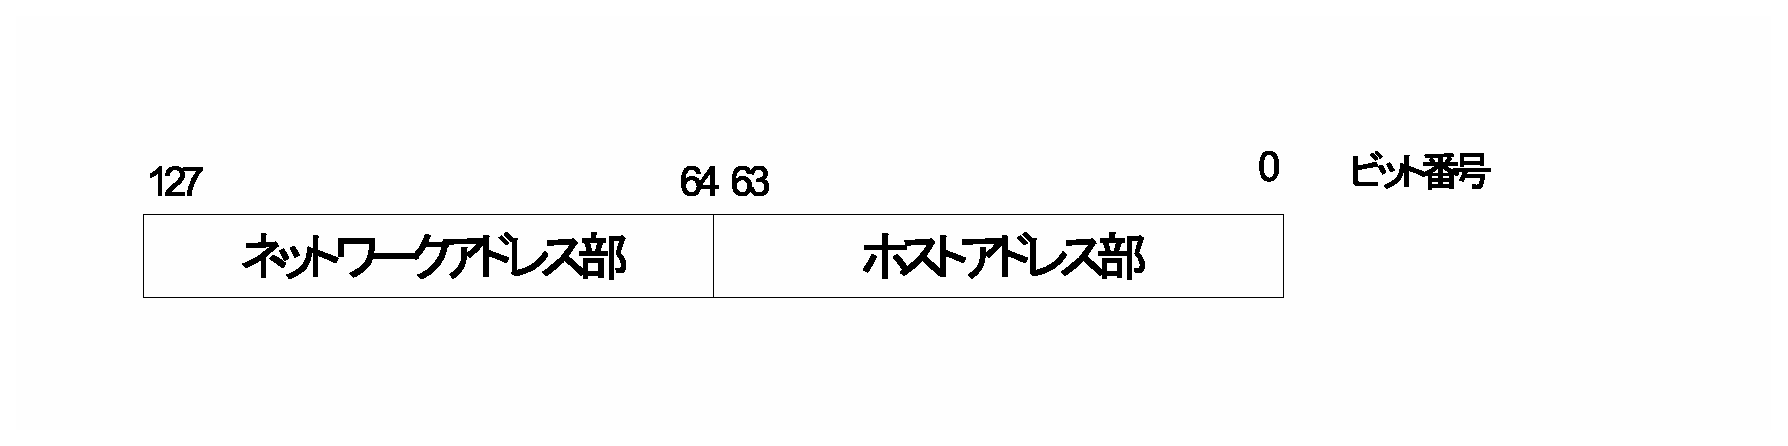
\includegraphics[width=12cm,clip]{draw/ip6addr.eps}
	\caption{IPv6アドレスの構造}
	\label{fig:ipaddr}
\end{figure}


IPv6では、ネットワークアドレスとホストアドレスの区切りは、1ビット単位で設定することができる。だが、IPv6の機能である、IPv6アドレスの自動割り当て機能を利用しようとする場合、ネットワークアドレス64bit、ホストアドレス64bitであることがRFC4291によって求められている。

そのため、一般的なネットワーク設定では、先頭64bitをネットワークアドレスとして扱い、残り64bitをホストアドレスとして設定する。この理由から、実用上は64bitで区切られる、と考えて良いだろう。

\subsection{IPv6アドレスの表記}
IPv6のアドレスは、128bit長ある。仮にIPv4と同じやり方で表記したとすると、32組の10恣意の数字が並ぶことになる。そこで、IPv6では、ビット列を16bitごとに区切り、それぞれを16進数で表記する。つまり、16進数4桁が8組並んだものが、IPv6のアドレスとなる。

実際の表記では、4桁の16進数8組を、コロンでれんけつしてひとつのアドレスとする。

0と1が128個並ぶことになるのででビット列は省略するが、たとえば、2001:0db8:0000:0000:0001:0000:0000:0123というように、IPv6アドレスはあらわされる。


\subsection{IPv6のプレフィクス長}
IPv6では、ネットワークアドレスとホストアドレスの区切りを示すのに、ネットマスク表記ではなくプレフィクス長を用いる。IPv6の場合は128bitの長さがあるため、仮にネットマスク表記をすれば、FFFF:FFFF:FFFF:FFFF:00000:0000:0000:0000というように、とても長くなってしまうためだ。この場合、プレフィクス長を用いて/64と表現する。

IPv6のアドレスは、128bitである。そのため、プレフィクス長は最大で/128ということににある。
IPv4と同様に、ビット長である/128を用いるときは、ネットワークアドレスの範囲でなく、そのIPアドレスただ一つをあらわす。


\subsection{IPv6アドレスの省略記法}
IPv6アドレスは、きちんと書くと長い。そのため、少しでも短く記述するための省略記法が設定されている。その省略は、以下のルールで行わうことが許されている。

\paragraph{16bitごとの先頭の0は省略できる}
16bit区切りごとの、先頭の0は省略することができる。たとえば、IPアドレスの先頭が32bitが2001:0db8:であるとすれば、2001:db8:というように、0db8の先頭の0省略して記述することができる。

\paragraph{連続する0は一箇所だけ省略できる}
16bitの区切りで、0000と表現される部分があれば、一箇所だけ表記そのものを省略してかまわない。また、それが連続して現れれば、まとめて省略することができる。2001:0db8:0000:0000:0000:0000:0000:0123であれば、2001:db8::123というように表記する。その省略部分は::と、コロン二つで記述する。

この省略規則では、一箇所以上の連続があった場合は、そのうちの一箇所だけを省略可能となる。た先に例として用いた、、2001:0db8:0000:0000:0001:0000:0000:0123というアドレスを省略する場合で考えてみよう・、

2001:db8::1::0000:0000:123と書くか、2001:db8:0000:0000:1::123と書くか、どちらにでも表記することができる。だが、2001:db8::1::123という表記をすると、省略部分に挟まれた0001が、128bitのどこにはいるかわからなくなってしまう。

この省略記法を用いいる場合、128ビット全てが0のアドレスは::、一番最後のビットだけ1のアドレスは::1と表記することができる。詳しくは後述するが、それぞれ、デフォルトルートをあらわすアドレスと、ループバックアドレスに付けるアドレスである。

\subsection{IPアドレスの分類}

IPアドレスには、どのような宛先を表すかでいくつかの種類がある。ユニキャスト、マルチキャスト、ブロードキャスト、そして、IPv6で追加された概念として、エニーキャストである。それぞれについて説明をしていく。

\subsubsection{ユニキャストアドレス}

\begin{figure}[htbp]
	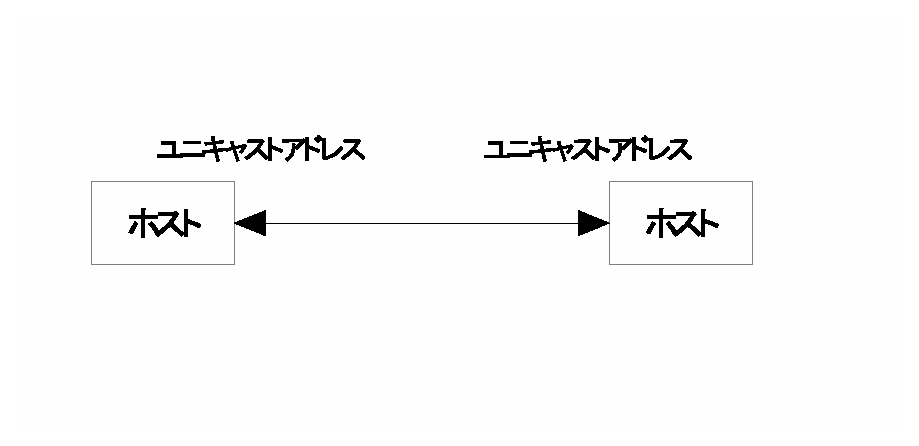
\includegraphics[width=12cm,clip]{draw/unicast.eps}
	\caption{ユニキャストアドレス}
	\label{fig:unicast}
\end{figure}

ユニキャストアドレスは、あるネットワークの範囲で、たった一つのネットワークインタフェイスを表すためのアドレスである。あるユニキャストアドレス当てに送信されたパケットは、そのアドレスに定められたネットワークの範囲において、ただ一つのネットワークインタフェイスに到達する。つまり、ただ一つのホストを宛先としたい場合に、ユニキャストアドレスを使用する。

IPv4、IPv6の両方に、ユニキャストアドレスの概念がある。


\subsubsection{マルチキャストアドレス}
\begin{figure}[htbp]
	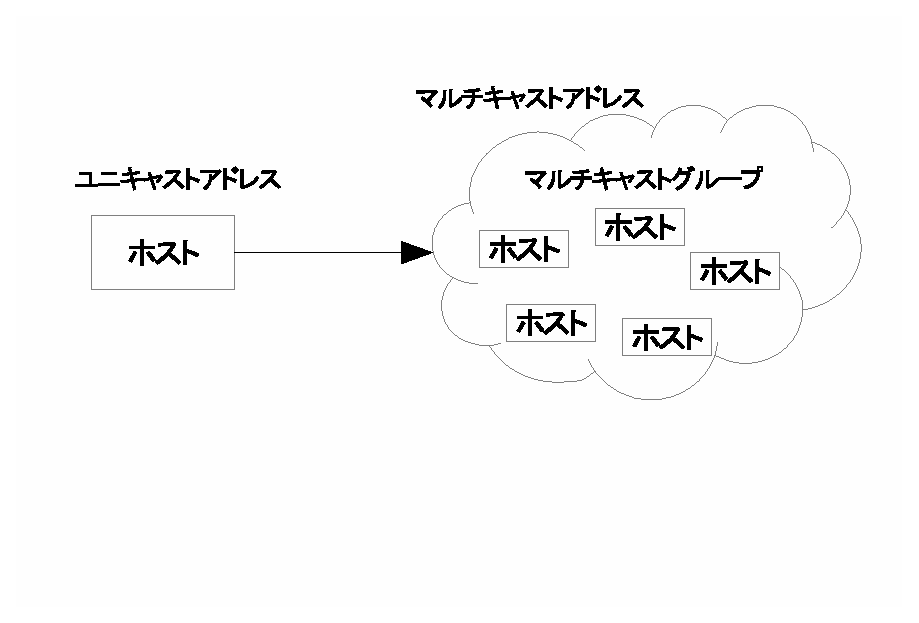
\includegraphics[width=12cm,clip]{draw/multicast.eps}
	\caption{マルチキャストアドレス}
	\label{fig:multicast}
\end{figure}

マルチキャストアドレスは、あるネットワークの範囲で、ネットワークのインタフェイスのグループを表すアドレスである。あるマルチキャストアドレス宛に送ったデータグラムは、同じマルチキャストアドレスを持つネットワークインタフェイス全てに到着する。あるグループに属する全てのホストに対して、同じデータを送信したい場合にマルチキャストアドレスを指定する。

マルチキャストアドレスは、その性質から、トランスポート層のプロトコルで、TCPのようなコネクション指向のものを使用することはできない。

マルチキャストは、IPv4では後で拡張された概念である。一方、IPv6では最初から導入されており、インターネットプロトコル層での制御に用いられる。

\subsubsection{ブロードキャストアドレス}
IPv4で、同じネットワーク内の全てのホストを表すアドレスである。ブロードキャスト宛ての通信は、そのネットワークの中の全てのホストが受信する。そのため、放送(ブロードキャスト)アドレスと呼ぶわけだ。

IPv4では、ホストアドレス部分のビットを全て1にすると、ブロードキャストアドレスとなる。たとえば、192.168.1.0/24というネットワークのブロードキャストアドレスは、ホストアドレス部分である下位8bitをすべて1にした192.168.1.255となる。

IPv6には、ブロードキャストアドレスはない。ではどのようにしているのだろうか。IPv6では、ブロードキャストに相当する宛先を利用したい場合は、「全てのホスト宛のマルチキャストアドレス」を使用する。そのため、IPv6にはブロードキャストはない。

\subsubsection{エニーキャストアドレス}

\begin{figure}[htbp]
	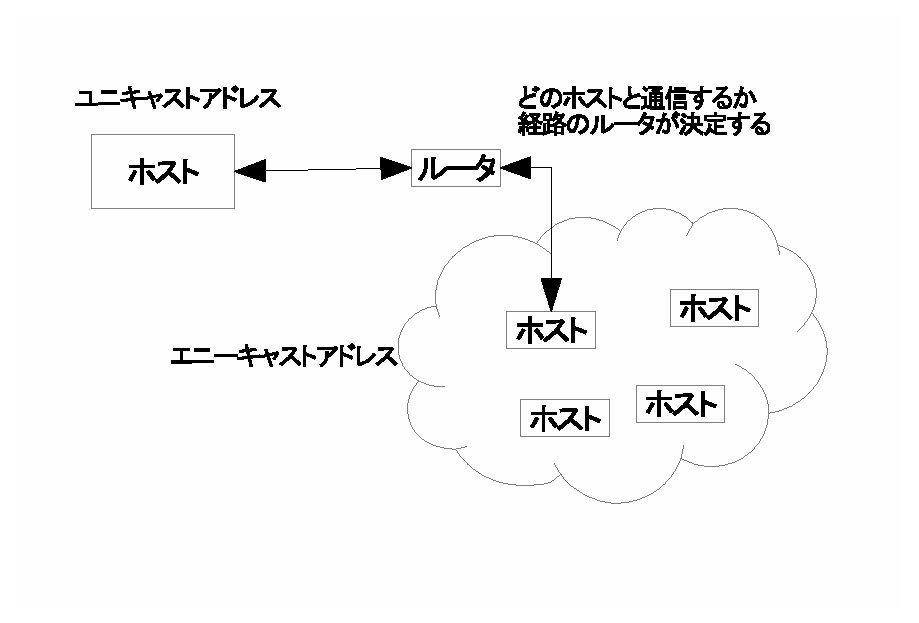
\includegraphics[width=12cm,clip]{draw/anycast.eps}
	\caption{エニーキャストアドレス}
	\label{fig:anycast}
\end{figure}

エニーキャストアドレスは、IPv6で追加されたアドレスである。

エニーキャストアドレスは、マルチキャストアドレスのように、あるネットワークの範囲で、ネットワークインタフェイスのグループを表す。だが、エニーキャストアドレス宛に送信したデータグラムは、そのグループに属するネットワークインタフェイスのどれかひとつが受信する。どのインタフェイスと通信するかは、経路の途中にあるルータが決定する。

エニーキャストでは最終的に一対一の通信となるため、宛先をエニーキャストアドレスとして、TCPを使用することもできる。だが、エニーキャストは通信相手が時間や状況の変化によって変わることがある。その場合、TCPのコネクションが切断され、新しい通信相手とハンドシェイクからやり直すことになってしまう。

そのため、データグラム型のUDPをトランスポート層のプロトコルとして使用することが多い。

エニーキャストアドレスは、たとえばネットワーク内のNTPやDNSサーバのように、最終的にネットワークに複数あるホストのどれが応えてもいい場合に使用する。たとえば、NTPサーバのグループにエニーキャストアドレスを付けておけば、NTP問い合わせに対して、エニーキャストアドレスを持ついずれかのホストが応答する。

\section{グローバルなアドレスとプライベートなアドレス}

ユニキャストのIPアドレスには、世界中でユニークであり、インターネット経由であるセス可能となるグローバルなアドレスと、プライベートなネットワークのみで使用するために範囲が設定された、プライベートなIPアドレスとに分けられる。

グローバル穴IPアドレスとプライベートなIPアドレスとは、用いるIPアドレスの範囲が異なる。

\subsection{ネットワークのスコープ}
あるネットワークの範囲という概念はどのようなものだろうか。それは、あるユニキャストアドレスやマルチキャストアドレスが、唯一のものとして判定される範囲ということである。これを、ネットワークのスコープとよぶ。

たとえば、LANの同じセグメントの中というスコープ、ルータで複数ネットワークが接続されたキャンパスネットワークの中というスコープ、インターネットで世界唯一として特定できるスコープ、などが考えられるだろう。

スコープは、たとえばルータが中継する、またはあるアドレス宛の通信を中継する、あるいは中継しないという判断の基準となる。

\subsection{IPv4のグローバルアドレス}
IPv4のグローバルなIPアドレスは、次に説明するプライベートアドレスの範囲、クラスD,クラスE、そして、特別なアドレスとして予約されている領域を除いた全てである。スコープという言葉を使えば、ワールドワイドなスコープである。

IPv4アドレスは元々、ARPA Netという、当時のグローバルなネットワークの中でユニークなインタフェイスを表すアドレスであった。プライベートアドレスの範囲などは、すべて後付けの概念である。

IPv4でグローバルなIPアドレスの割り当てを受ける際は、1つのインタフェイスに対して、ネットワークアドレスとホストアドレス全ての割り当てを受けるか、ネットワークに対して、ネットワークアドレス部分の割り当てを受けるかのどちらかになる。

前者は、割り当てられたひとつのインタフェイスのみが、グローバルなIPアドレスを持つ。後者は、ネットワークに対してネットワークアドレスを割り当てられるので、ホストアドレス部分は割り当てを受けた範囲で、任意に設定することができる。

\subsection{IPv4のプライベートアドレス}

IPv4アドレスには、外部に直接接続しないネットワーク(実験用、イントラネットなど)で、特に割り当てを受けなくても自由に使用できるIPアドレスの範囲が決まっている。このIPアドレスの範囲を、プライベートアドレスと呼んでいる。

プライベートアドレスのスコープを送信元とするデータグラムの宛先は、プライベートアドレスの割り当てられたホスト・ネットワークのみとなる。グローバルスコープのホストと直接通信することはない。

プライベートアドレスは、クラス毎に以下のように予約されている。

\begin{table}[hbtp] \caption{プライベートアドレスの範囲} \label{privateaddress}
\begin{center}
{\footnotesize
\begin{tabular}{lll} \toprule
クラス & ネットワークアドレス & アドレス範囲\\ \midrule
A & \verb+10/8+ & \verb+10.0.0.0-10.255.255.255+\\
B & \verb+172.16/12+ & \verb+172.16.0.0-172.31.255.255+\\
C & \verb+192.168.0/16-192.168.255/24+ & \verb+192.168.0.0-192.168.255.255+\\ \bottomrule
\end{tabular}
}
\end{center}
\end{table}

\subsection*{}
\begin{itembox}[l]{いもうとコラム IPv4のプライベートアドレスからのインターネットアクセス}
IPv4のプライベートスコープからグローバルスコープへ、直接の通信は行われません。でもこれは、通信をしてはならないという意味ではありません。

プライベートスコープのホストがグローバルスコープにアクセスする場合は、グローバルスコープのIPアドレスを用意し、そのアドレスを持つホストに、代わりにアクセスしてもらいます。プライベーツスコープのホストは、その結果をもらうことで、インターネットアクセスを行うわけです。

このように、アクセスを中継する役目を持つホストをプロキシといいます。プロキシにはアプリケーション層の代理アクセ宇を行うのプロキシ、トランスポート層の代理アクセスを行うNAPT(Network Address and Port Translation)もしくはIP masquarade、インターネットプロトコル層の代理アクセスを行うNAT(Network Address Translate)というようなものがあります。

\end{itembox}

\subsection{IPv6のグローバルアドレス}

\begin{figure}[htbp]
	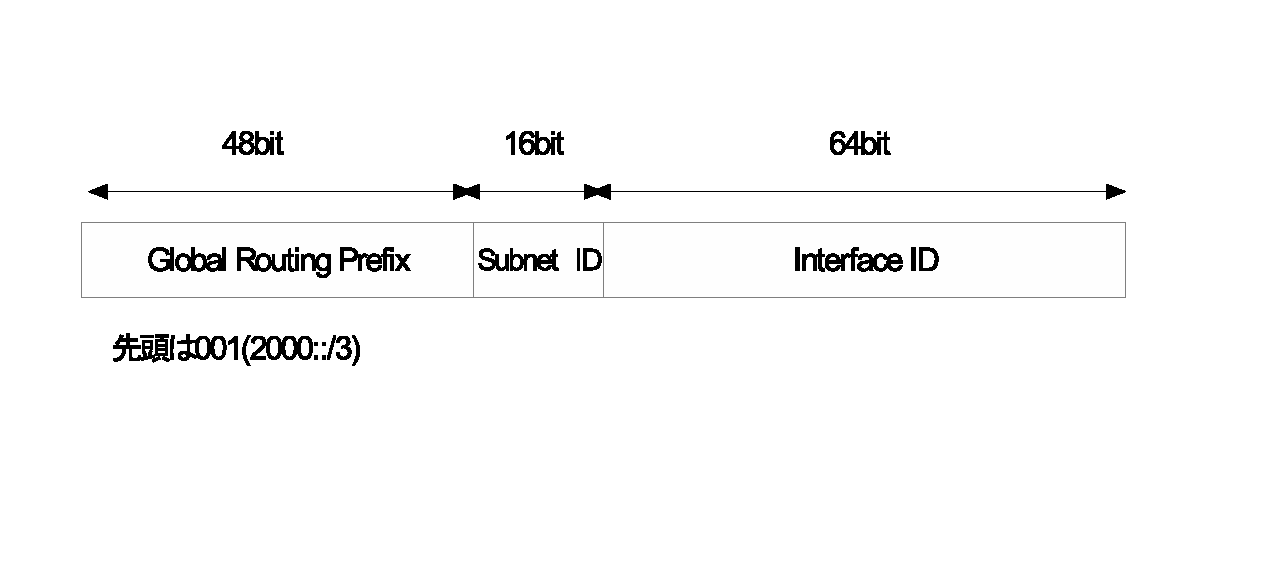
\includegraphics[width=12cm,clip]{draw/gua.eps}
	\caption{グローバルユニークアドレス}
	\label{fig:gua}
\end{figure}


IPv6によって世界で唯一のホストを特定するためのアドレスであり、発信元や宛先に指定したパケットが、インターネットに中継されるアドレスである。

先頭から48bit部分は、プロバイダによって割り当てられる。そのため、特に、グローバルプレフィクスとよんでいる。次の16bitはサブネットIDとよばれ、ユーザがサブネットを定義するために、任意に設定することが許される部分である。

だが、サービスによっては、プロバイダが、64ビットのプレフィックスを割り当ててくることがある。この場合、ユーザはサブネットを設定することはできない。

グローバルユニークアドレス発信元並びに宛先としたデータグラムは、全てのルータで中継を受けることができる。

\subsection*{}
\begin{itembox}[l]{いもうとコラム TLAとNLAとSLA}
古いIPv6の規格では、グローバルユニークアドレスは、TLA、NLA,SLAという部分による階層構造を取るというように定義されていました。。これは、インターネットサービスプロバイダ間でのアドレス割り当てが階層構造となることを想定したものでした。

ですが、現在は、グローバルプレフィクスとサブネットIDという、2段階の構造となっています。

\end{itembox}

\subsection{IPv6のリンクローカルアドレス}

\begin{figure}[htbp]
	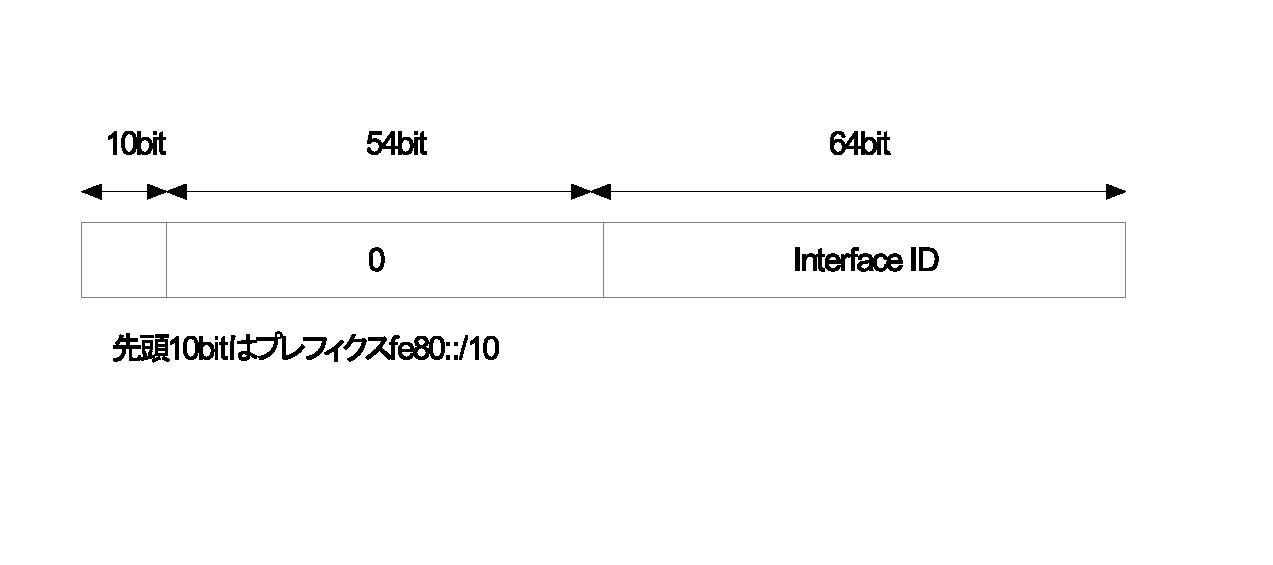
\includegraphics[width=12cm,clip]{draw/lla.eps}
	\caption{リンクローカルアドレス}
	\label{fig:lla}
\end{figure}

IPv6のリンクローカルアドレスは、ネットワークアクセス層でいうところの、ひとつのネットワークをスコープとするアドレスである。つまり、リンクローカルスコープを用いた通信は、ルータで中継されることはない。そのため、リンクローカルアドレスには、サブネットIDのフィールドが存在しない。

リンクローカルアドr巣は、FE80::/10が割り当てられている。

また、リンクローカルアドレスを宛先に使用する場合、その通信の発信元のインタフェイスを併記する場合がある。

ここで気をつけなければならないのは、リンクローカルアドレスは、同一ネットワーク内での通信に使うためのアドレスであり、IPv4のプライベートスコープのアドレスにそうと酢売るものではないことである。


\subsection{IPv6のユニークローカルアドレス}

\begin{figure}[htbp]
	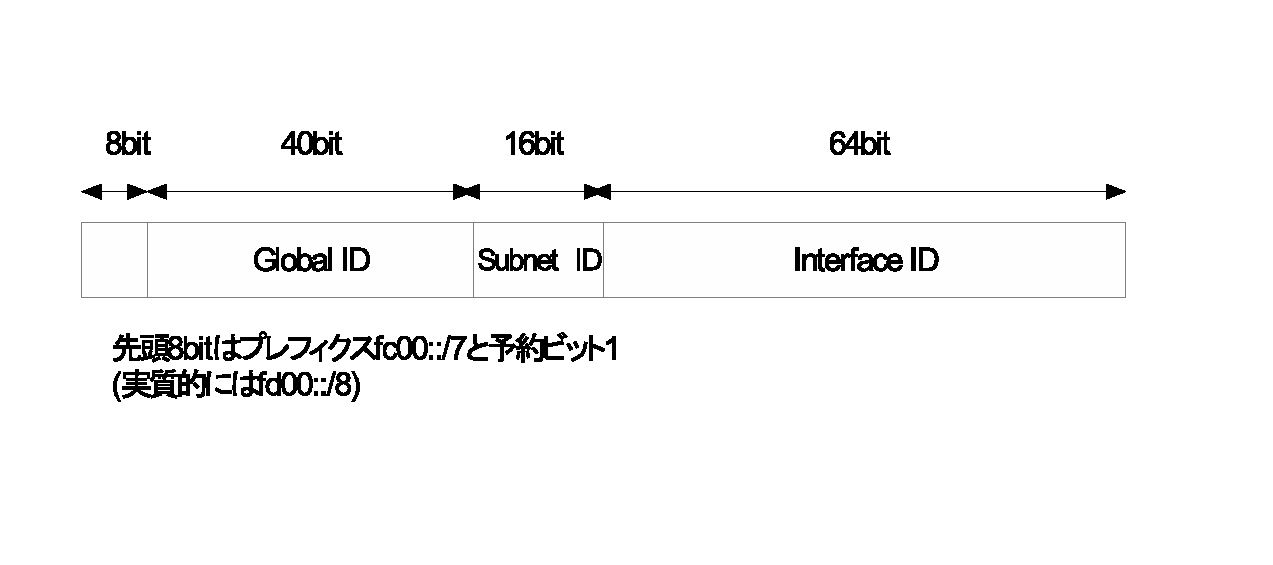
\includegraphics[width=12cm,clip]{draw/ula.eps}
	\caption{ユニークローカルアドレス}
	\label{fig:ula}
\end{figure}

IPv4にも、プライベートスコープアドレスがある。それが、ユニークローカルアドレスである。

元々はIPv6のアドレスは、グローバルユニークアドレスと、リンクローカルアドレスだけであった。あが、申請やプロバイダとの契約無しで、LANの中で使用可能なIPアドレスがあった方が便利であること、ネットワークインタフェイスにグローバルユニークアドレスを割り当てていると、ISPを変更することでプレフィクスが変更され、そのネットワーク内の機器全てで設定変更が必要になること、といった、実用面での理由から、ユニークローカルアドレスが制定された。

ユニークローカルアドレスは、グローバルIDと同様に、グローバルIDとサブネットID、インタフェイスIDから構成される。グローバルID部分は、fc00::/7が割り当てられ、この範囲で規定の手順でランダムに生成することが推奨されている。

インターネットに、ユニークローカルアドレスを宛先や発信元とするデータグラムを送出することはできない。だが、それ以外の、LAN内部のルータは、ユニークローカルアドレスを経由した通信を中継することができる。

\section{IPv6のマルチキャストアドレス}

\begin{figure}[htbp]
	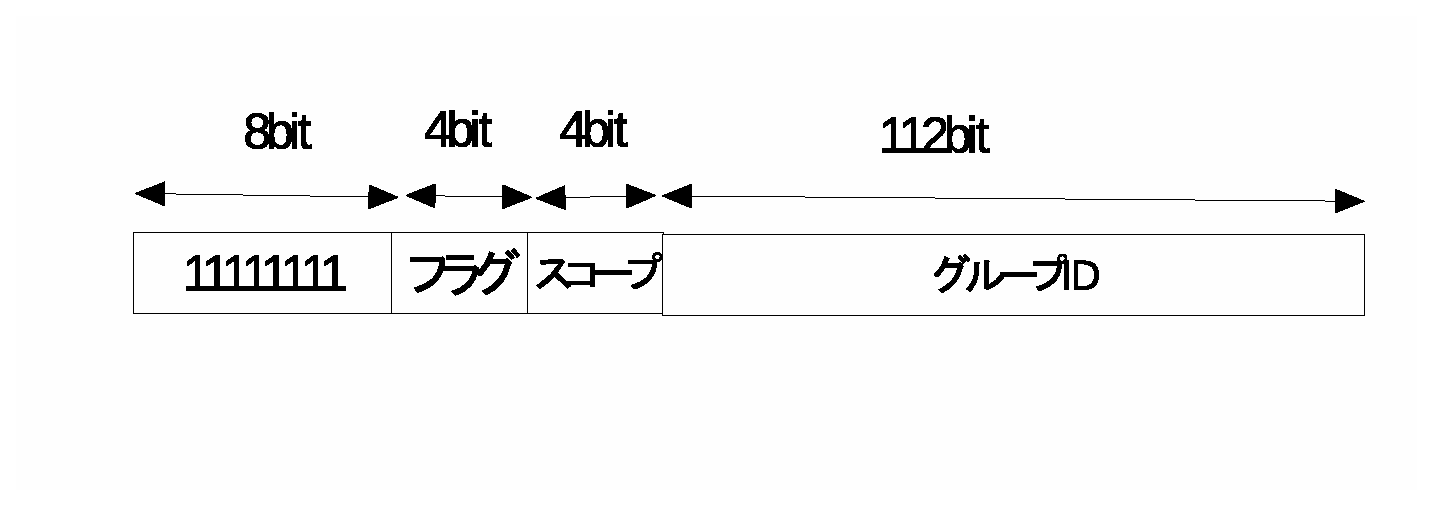
\includegraphics[width=12cm,clip]{draw/6multicast.eps}
	\caption{マルチキャストアドレス}
	\label{fig:6multicastaddr}
\end{figure}
マルチキャストアドレスは、ネットワークインタフェイスのグループを表すアドレスである。マルチキャストアドレスを宛先にしたデータグラムは、そのグループに属する全てのネットワークインタフェイスに届けられる。

IPv4ではオプションであったが、IPv6ではマルチキャストを積極的に利用する。ここでは、IPv6のマルチキャストについて、簡単に説明を行っていく。

マルチキャストアドレスは、おおまかに、プレフィクス部分と、グループID部分という構造を持つ。ユニキャストアドレスと違って、サブネットIDやインタフェイスIDはもたない。

また、マルチキャストアドレスでも、ユニキャストアドレスと同様に、スコープの考え方がある。これは、そのマルチキャストアドレスが存在できるネットワークの範囲が、スコープである。

IPv6のマルチキャストアドレスは、先頭8bitが必ず11111111、つまり、十六進数でFFとなる。次の4bitは、IANAによって割り当てられたアドレスであれば0、それ以外のテンポラリなものなら1を割り当てる。

スコープは4bitのフィールドで表される。このフィールドの数字は、そのまま、発信元のインタフェイスとルータを超えられる回数をイメージすれば良い。ノードローカルスコープは最大ホップ数が1なので、ホストが持つネットワークインタフェイスを越えられない。リンクローカルスコープは、最大ホップ数が2なので、ルータを越えることができない。そう考えれば何となくイメージできるだろう。

のこり112bitが、グループIDであり、あて先をあらわす。

だが、厳密には、インタフェイスローカル、リンクローカル、グローバルを除くスコープについては、管理者がIPv6ヘッダの最大ホップ数(ホップ制限)フィールドを適切に設定して、伝播範囲を制御する必要がある。

\subsection{インタフェースローカル}
インタフェースローカルスコープは、あるノード(ホスト)をスコープとする。古い資料ではノードローカルと記載されている場合がある。スコープのIDは1となる。

インタフェースローカルをいわば、マルチキャスト版のループバックアドレスである。では、どこがマルチキャストかのかというと、プロセスの待ち受けをグループ化する。

たとえば、スコープがインタフェースローカル、グループIDが101のNTPの場合、fe01::101は、自分自身の上で動いている全てのNTPサーバのプロセスが接続待ちしているポートを宛先とする。

また、ff00::1は、ノードローカルの全ノードが宛先であり、マルチキャスト版のループバックアドレスとなる。

\subsection{リンクローカル}
ルータ越えしない、同じネットワークの範囲でのマルチキャストである。スコープIDは2となる。

ff02:101は、ルータを越えずにアクセスできる全てのNTPサーバが宛先となる。
また、ff02::1であれば、ルータ越えしない、同じネットワークに接続されている全てのホストとなる。IPv4での、ブロードキャスト宛ての通信は、IPv6では、ff02::1を宛て諭したマルチキャスト通信となる。

IPv6が有効となっていれば、すべてのインタフェイスは、リンクローカルアドレスff02::1と、後ほど説明するNDP(Neiborhood Discovery Protocol(に用いられる要請ノードアドレスFF02::1:FF00:0000/104という二つのマルチキャストアドレスを持つ。要請ノードアドレス下位24bitは、ユニキャストIPv6アドレスのホストアドレス部分の下位3バイトとなる。


\subsection{組織ローカル}
組織ローカルスコープは、同一組織のネットワークをスコープとするマルチキャストアドレスである。スコープIDは8となる。

たとえば、同じ組織のネットワークにあるNTPサーバ全てにアクセスするなら、ff08::101が宛先となる。

組織ローカルスコープよりも範囲が狭い、サイトローカルスコープという概念もあるが、現在は推奨されないマルチキャストアドレスとされている。

\subsection{グローバル}
文字通り、インターネット全体をスコープとするマルチキャストアドレスである。だが、ヘッダで最大ホップ数が設定されるので、世界中に限りなく伝播していくわけではない。そうでないと、マルチキャストの転送ループが生じて、ネットワークが輻輳する。


\section{特別な意味を持IPアドレス}

IPアドレスに関した話題の最後に、特別な意味を持つユニキャストIPアドレスの説明を行なおう。これらのIPアドレスは、ネットワークやアプリケーションの設定でよく使用されるものである。

\subsection{デフォルトルートあるいは全ネットワーク}

IPv4で0.0.0.0/0もしくは、0.0.0.0/0.0.0.0と、IPv6で::、つまり全ビットを0として記述されるIPアドレスは、以下の二つの意味を持つ。

\begin{itemize}
\item デフォルトルート設定のときに、「自分と同じネットワークアドレスを持つIPアドレス以外のアドレス全て」を 表すアドレス
\item ネットワーク対応アプリケーションの設定などで、「全てのネットワーク」を表すアドレス
\end{itemize}

前者の意味で使用される場合は、ルートの設定がされていない宛先全て、という意味になる。また、後者の意味で使用されるときは、通信相手に関わらず同じ設定を適用したいときに用いられることが多い。

\subsection{ループバックアドレス}

IPv4で127/8もしくは127.0.0.0/8、IPv6で::1/128というように書かれる、クラスAのIPアドレスで、最大の番号を持つネットワークアドレスは、そのホスト自身を表すものとして予約されている。自ホストから送信された127/8宛のデータグラムは、ローカルループバックインタフェイスに送られる。

ローカルループバックは、便宜上127.0.0.1を使用することが多い。だが、ネットマスクを見て分かるとおり、127.0.0.0-127.255.255.255の、 16Mi個のIPアドレスが全て自分のローカルループバックインタフェイスを指す。実際、この範囲のどのIPアドレスに対して通信を行っても、ローカルループバックに到達するし、そのように実装しなければならない。

ループバックインタフェイスには、必ずループバックアドレスが割り当てられる。

\subsection*{}
\begin{itembox}[l]{いもうとコラム ループバックインタフェイスに割り当てるアドレス}
ループアバックインタフェイスには、必ずループバックアドレスを割り当てます。ですが、ループバックインタフェイスにはループバックアドレス以外を割り当ててることができます。

ループバックインタフェイスもネットワークアクセス層のインタフェイスのひとつなので、ループバックインタフェイス以外のアドレスを割り当てることも可能です。
\end{itembox}


\subsection{リミテッドブロードキャストアドレス}

255.255.255.255は、IPv4アドレスのリミテッド・ブロードキャストアドレスと呼ばれる、特別なブロードキャストアドレスである。自分のIPアドレスが分からないネットワークインタフェイスが、そのネットワーク内にデータグラムを送信するときに使用する。例えば、IPアドレスをサーバから配布してもらうDHCPで、IPアドレスがまだ配布されていないクライアントが、DHCPサーバと最初の通信を行うのに使用する。

同じネットワーク(ネットワークアクセス層のプロトコルで通信できるネットワーク)の全てのホストを宛先としてデータグラムを送信するために使用することは推奨されない。

IPv6では、このような場面ではマルチキャストアドレスを用いる。


\subsection{ドキュメント用アドレス}
IPv6に関するドキュメントを記述するためのアドレスとして、2001:db8::/32は予約されている。そのため、これをプレフィクスとして持つアドレスを発信元や宛先とするデータグラムを、インターネットに中継してはならない。







\section{データグラムとヘッダ}

ここまでで、インターネットプロトコルにおいて、バケツリレーのルールと、バケツリレーの宛先となるネットワークと、その中のホストを判別する方法を説明した。ここからは、バケツの中身、つまり、インターネットプロトコルでデータを送出する単位であるデータグラムを見ていくことにしよう。

インターネットプロトコル層では、データの単位を「データグラム」と呼ぶ。データグラムは、宛先のIPアドレス、送信元のIPアドレスなどの情報が記載されたヘッダと、宛先に届けるデータである、ペイロード部分から構成される。

ヘッダは、発信元IPアドレスと宛先IPアドレスを記入するフィールドとがある。TCP/IPのモデルで、IPアドレスを記載するのはIPヘッダだけである。

\subsection{IPv4ヘッダ}
IPv4のヘッダは、以下のような構造をしている。
オプションは必要に応じて追加し、32ビット境界になるようにパディングされる。そのため、ヘッダ部分は、20Byte以上で 4byte刻みの大きさとなる。

それぞれのフィールドの意味は、必要になった場面で説明しよう。
\begin{figure}
	\includegraphics[width=14cm,clip]{draw/ipheader.eps}
	\caption{IPv4ヘッダ}
	\label{fig:ipheader}
\end{figure}

\subsection{IPv6ヘッダ}

\begin{figure}
	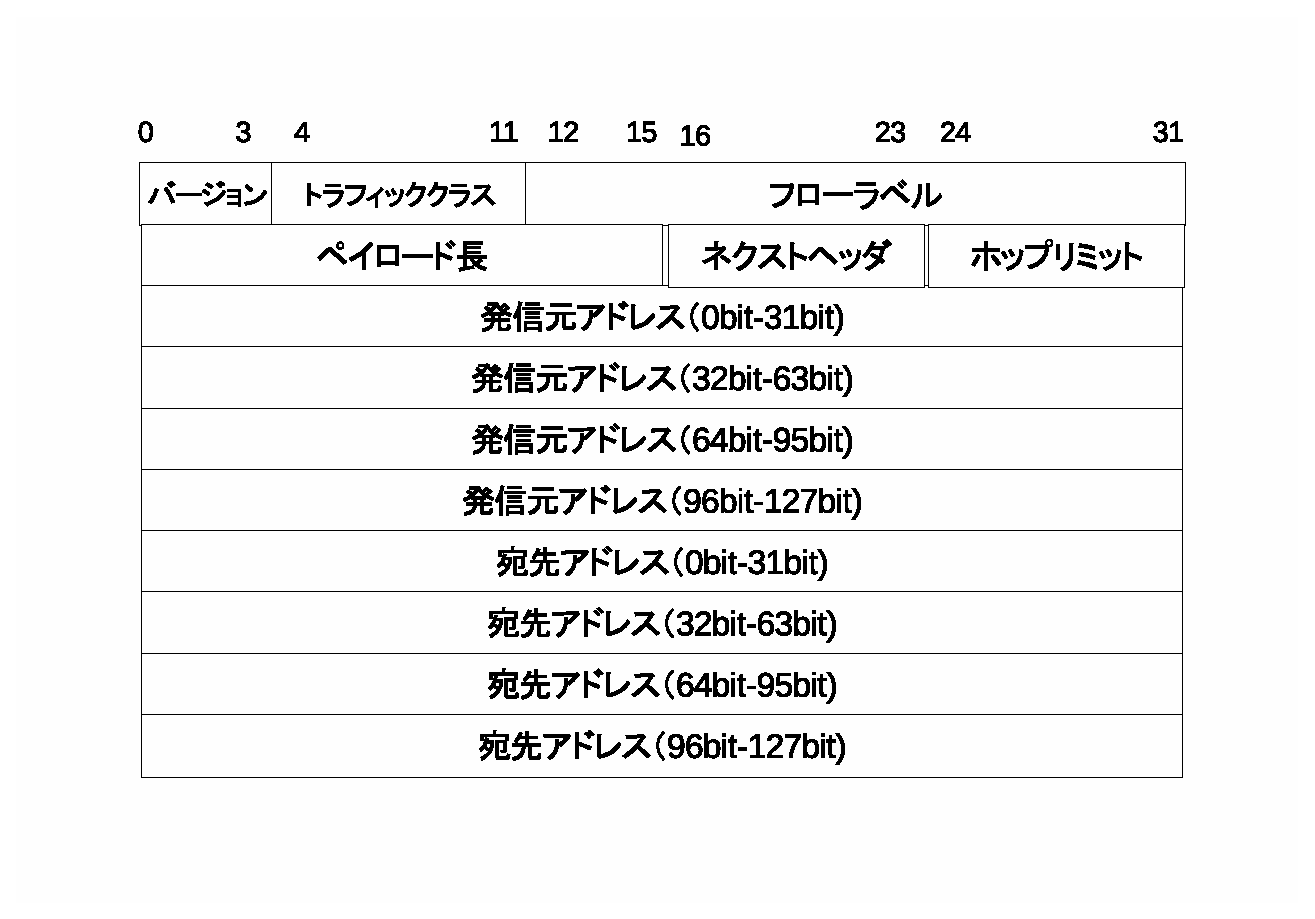
\includegraphics[width=14cm,clip]{draw/ipv6header.eps}
	\caption{IPv6ヘッダ}
	\label{fig:ipv6header}
\end{figure}

IPv6ヘッダは、図\ref{fig:ipv6header}ような構造をしている。チェックサムフィールドは、ネットワーク層やトランスポート層でデータの検査が行われることから、IPv6では省略された。それによって、サイズは大きいが構造はシンプルになっている。


\subsection{データグラムの最大の大きさ}
データグラムを実際に伝送するのは、ネットワーク内の通信を担当するネットワークアクセス層である。そのため、ヘッダとデータからなるデータグラムのサイズの最大の大きさは、ネットワークアクセス層の仕様に依存する。

また、ネットワークアクセス層に依存しないデータグラムの最大サイズは、全データ長フィールドが16ビットなので、64Kibyteまでとなる。

IPv4では、全データ長フィールドは、ヘッダとデータの合計のサイズを入れる。そのため、実際に64Kibyteきっちりデータ部分にできるわけではない。

IPv6では、ペイロード長フィールドは、ヘッダを含まない、ペイロード部分のみの大きさとなる。これは、IPv6では、ルータ巻の転送によって、全てのヘッダの長さがかわることがあるためである。

\subsection{ネットワークバイトオーダと htonl()}

IPアドレスは、32ビット(4byte)を単位としたビット列としてネットワークアクセス層に渡される。このときの送出順は、0ビット目(図\ref{fig:ipheader}の左側)から31ビット目(図\ref{fig:ipheader}の右側)にむけて「ビッグ・エンディアン」方向となる。これを、ネットワーク・バイトオーダという。

だが、x86系CPUなどは、24ビット~31ビット、16ビット~23ビット、8ビット~16ビット、0ビット~7ビットという、バイト単位で見たときにネットワークバイトオーダと逆順にメモリにコピーする仕様となっている。このような環境をリトル・エンディアンという。

そのため、プログラミングでIPアドレスを\verb+sockaddr_in+ 構造体にコピーする際に、\verb+htonl()+ という関数で、IPアドレスのビット列を、ネットワークバイトオーダで出力されるよう順番を入れ替えてから渡す。

一方、PowerPCやColdFireなど、ビッグエンディアンな環境では \verb+htonl()+ は不要なように思われる。だが、コードの移植性を考えて、常に\verb+htonl()+ を使用しておくようにする。\footnote{エンディアン変換の必要のない環境では\verb+htonl()+ は何もしないマクロとして定義されている。}


\subsection{IPv4ヘッダの最大・最小の大きさ}

データグラムのヘッダは、20byte以上の大きさで4byte(ワード長)刻みになる。では、そのヘッダの最大の大きさはいくつになるであろうか。

結論を言えば、最大の大きさは60byteとなる。これは、「ヘッダ長」フィールドが4bitであり、符号無しで最大値が15であることに由来する。ヘッダの大きさは、word(32bit、つまり4byte)単位で表される。

逆に、最小の大きさのヘッダは20byteとなる。この場合は5ワードになるため、ヘッダ長フィールドには5が記載される。

だが、実際のところ、IPヘッダのオプションフィールドが使用されることはほとんどない。IPv4ではヘッダ長フィールドがほとんど使用されなかったため、 IPv6では、IPヘッダを固定長として、ヘッダ長フィールドが廃止された。

\subsection{IPv6ヘッダの最大・最小の大きさ}
IPv6ヘッダは、サイズ固定である。その大きさは、40byteとなる。ただしこれは、ひとつのヘッダを可変長にしてオプション情報を詰め込むということをしない、という意味である。

IPv4では、可変長ヘッダが使われることはほとんどなかった。その知見から、IPv6ではヘッダの大きさは固定となっている。

\subsection{IPv6のネクストヘッダ}
\begin{figure}
	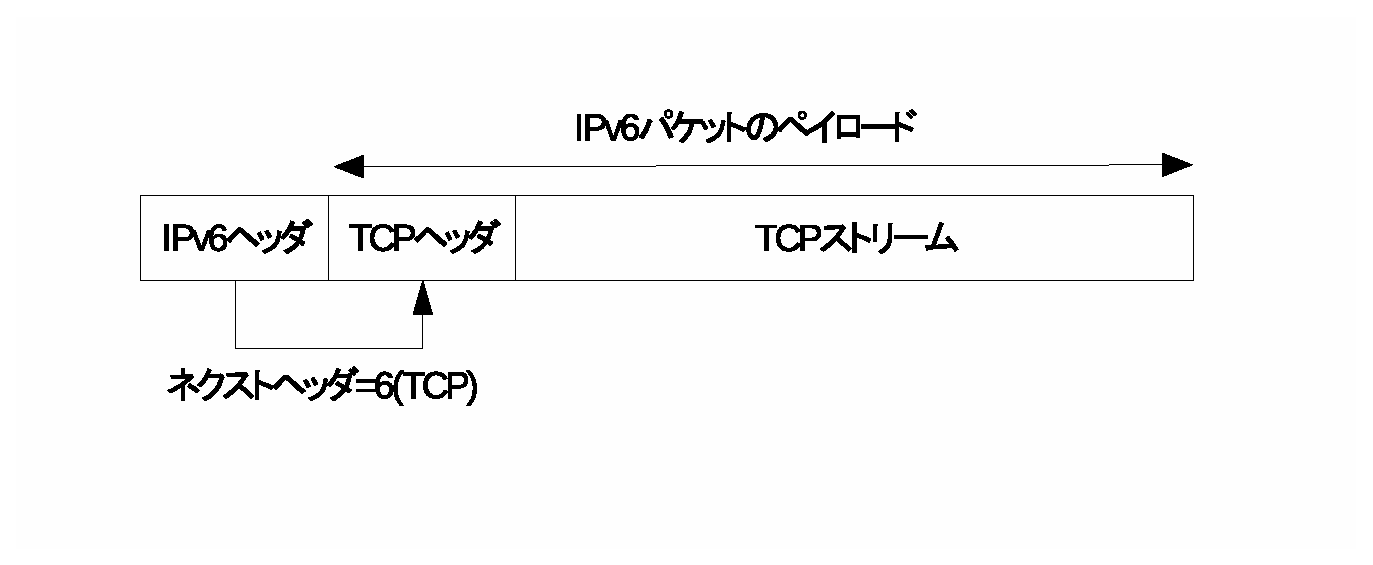
\includegraphics[width=14cm,clip]{draw/nextheader1.eps}
	\caption{IPv6のネクストヘッダ}
	\label{fig:ipv6nextheader}
\end{figure}

IPv6ヘッダには、ネクストヘッダというフィールドがある。これは、その名のとおり、IPv6ヘッダの跡に続く情報のヘッダがなにかをあらわすフィールドである。

では、ネクストヘッダフィールドは何に使われるのだろうか。このネクストヘッダは、IPv4のプロトコル番号フィールドとしての役割がある。ここにトランスポート層のプロトコルの番号を書けば、次のヘッダはトランスポート層のヘッダであり、ネクストヘッダ以降のペイロードをトランスポート層に渡す。

ここで、IPv6ヘッダの跡にトランスポート層のヘッダがくる、という点に注目しよう。インターネットプロトコル層のパケットの中では、IPv6ヘッダの後には必ず別のヘッダが来る。この概念を一般化すると、インターネットプロトコル層に関するオプションを、オプションヘッダという形で、ヘッダの後に続くヘッダとして定義する。それによって、各種オプションを一般化することができる。

この概念は、インターネットプロトコル層を中心にして考えたとき、複数のヘッダの後、上位層が運ぶべきデータがペイロードとして現れる、というものである。カプセル化の考えとも矛盾はしない。

では、オプションヘッダを使う例として、IPv6ジャンボデータグラムについて説明しよう。まず、インターネットプロトコル層は、IPv4,IPv6とも、ひとつのパケットの最大のサイズは64KiBである。これは、サイズのフィールドが16bitであるためである。

だが、IPv6ではジャンボデータグラムオプションという、それ以上の大きさのデータを転送するためのオプションがある。

IPv6のオプションヘッダには、ホップバイホップヘッダという、経路全てで参照されなければならないオプションヘッダがある。それに、ジャンボデータグラムの情報を付加して送信するわけだ。

ホップバイホップオプションをジャンボデータグラムのサイズ情報を格納するのに使用するとき、サイズ情報フィールドは、32bitとなる。このオプションを用いることで、最大4GiBの大きさのパケットを送信することが可能となる。

もうひとつ、IPsecのヘッダでも考えてみよう。IPsecのヘッダは、IPv4ではペイロード部分の先頭にあるビット列という考え方であったが、IPv6では、オプションヘッダのひとつとして、IPv6ヘッダの後に連結されるヘッダとなり、その後に暗号化されたペイロードが続く形となる。、

\begin{figure}
	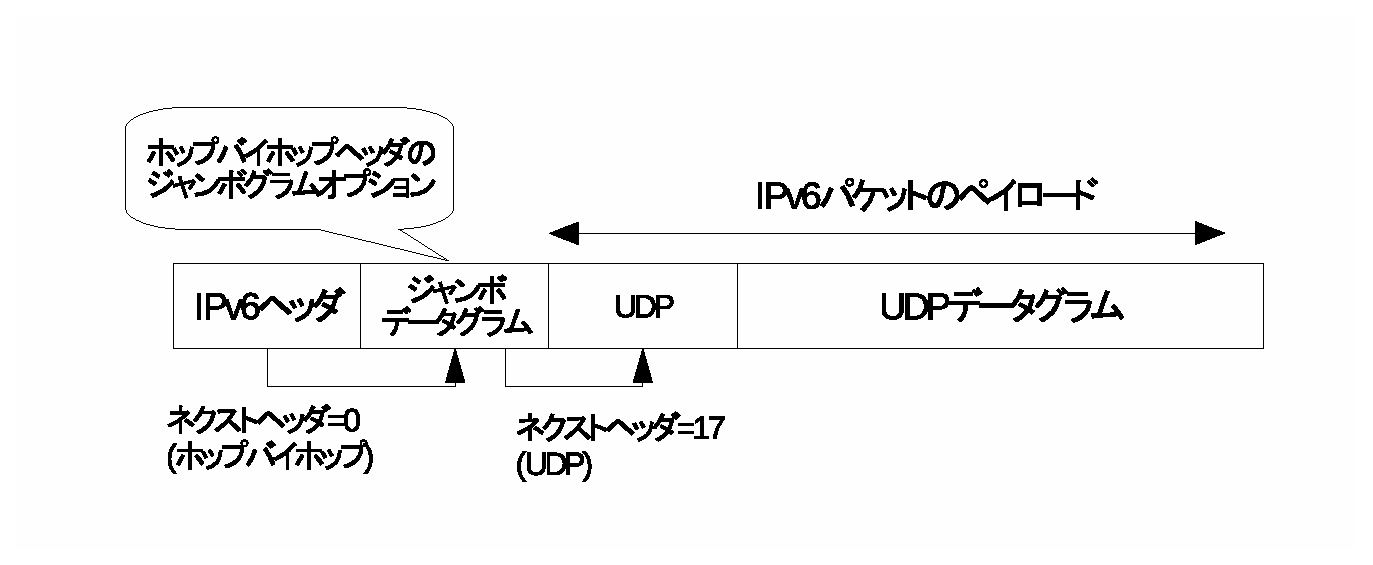
\includegraphics[width=14cm,clip]{draw/nextheader2.eps}
	\caption{IPv6のホップバイホップヘッダによるジャンボグラム}
	\label{fig:ipv6jumbogram}
\end{figure}


\subsection{ルータに中継してもらうデータグラムの宛先フィールド}

ルータに中継してもらうデータグラムのIPヘッダの宛先フィールドは、最終的に届けたいホストのIPアドレスとなる。間違えやすいが、ルータのIPアドレスではない。


では、そのデータグラムは、ヘッダにアドレスが書かれていないルータにどうやって届くのだろうか。ルータはネットワークアクセス層のプロトコルで通信できる場所に接続されている。つまり、ネットワークアクセス層のフレームの宛先が、ルータのネットワークインタフェイスとなるようにする。

インターネットプロトコル層では、自分宛でないデータグラムは、同じネットワークアドレス宛であれば、ネットワークアクセス層を利用して、相手ホストにデータグラムを伝送する。別のネットワーク宛であれば、ネットワークアクセス層を利用して、ルータにデータグラムを転送しようとするのは、ここまで説明したとおりである。

そして、インターネットプロトコル層レベルの通信は、その繰り返しで発信元からネットワークで接続された宛先に到着する。


\subsection{ルータに割り当てるIPアドレスに決まりはあるの?}
あるネットワークアドレスの範囲で、ルータ(デフォルトルート)に割り当てるホストアドレスをどれにするかという決まりはない。通常は、わかりやすくするために、そのホストアドレスの中でで一番小さい番号か、一番大きい番号かのどちらかから順番に割り当てることが多い

\section{IPv4の経路集約とCIDR}

IPv4では、ネットワークアドレスとホストアドレスをどこで分けるかの説明を思い出してほしい。先頭から8ビット目から30ビット目のどこかで分けると説明したときに、その方式の名前が CIDR(Classless Inter-Domain Routing)、であったことに違和感を感じなかっただろうか。

CIDRはその名の通り、元々は経路を集約する為に考えられたものであった。では、経路の集約とは何をすることだろうか。

たとえば、192.168.0.0/24のネットワークと192.168.1.0/24のネットワークが存在するとする。このとき、それぞれのネットワークが別々にに存在すれば、192.168.0.0./24に接続されたルータと、192.168.1.0/24に接続されたルータがそれぞれ必要になる。もちろん、経路も別々に記載し、設定しなければならない。

この例では二つのネットワークだけだから経路を全て記載してもたいしたことにならなかった。だが、これ世界規模になれば、経路を設定する手間が大変なことになる。そして、ルータが記憶すべき経路の量も大変なことになる。経路集約は、その負荷を減らす為の技術である。

ここまでの例でいくと、192.168.0.0/24と、192.168.1.0/24は、192.168.0.0/23というネットワークアドレスを持つネットワークの一部分、として扱う。つまり、外部から見たとき、192.168.0.0/24宛のデータグラムも、192.168.1.0 /24宛のデータグラムも、192.168.0.0/23というネットワークに接続されていることになっているルータに送ればいい。到着したデータグラムを、それぞれの宛先に応じて、どちらかのネットワークに転送するかは、最終的には192.1689.0.0/22のネットワークに接続されているルータの仕事となる。

では、なぜこういう方法をとることができるのだろうか。それは、IPヘッダのIPアドレスのフィールドには、ネットマスクの情報がないためである。つまり、データグラムがサブネットマスクの情報を持たないことを、恩恵として利用している。192.168.0.0/24及び 192.168.1.0/24以外のネットワークにあるホストは、このネットワークアドレスに対して送信するときに、これらのネットワークアドレスと 192.168.0.0/23を区別できない。

実際に、それぞれのネットマスクを適用したビットパターンで見てみよう。

\begin{table}[hbtp] \caption{ネットマスク23bitの場合} \label{mask23}
\begin{center}
{\footnotesize
\begin{tabular}{lll} \toprule
192.168.1.1/23 & バイナリ表記 & 十進表記\\ \midrule
ネットワークアドレス部 & \verb+11000000.10101000.00000000.00000000+ &192.168.000.000\\
ホストアアドレス部 & \verb+00000000.00000000.00000001.00000001+ & 000.000.001.001\\
IPアドレス & \verb+11000000.10101000.00000001.00000001+ & 192.168.001.001\\ \bottomrule
\end{tabular}
}
\end{center}
\end{table}

\begin{table}[hbtp] \caption{ネットマスク24bitの場合} \label{mask24}
\begin{center}
{\footnotesize
\begin{tabular}{lll} \toprule
192.168.1.1/24 & バイナリ表記 & 十進表記\\ \midrule
ネットワークアドレス部 & \verb+11000000.10101000.00000001.00000000+ & 192.168.001.000\\
ホストアアドレス部 & \verb+00000000.00000000.00000000.00000001+ & 000.000.000.001\\
IPアドレス & \verb+11000000.10101000.00000001.00000001+ & 192.168.001.00\\ \bottomrule
\end{tabular}
}
\end{center}
\end{table}

このように、ネットマスクの情報がなければ、この両社を区別する情報を、送信側が持つことはない。

\begin{figure}[htbp]
	\includegraphics[width=12cm,clip]{draw/cidr.eps}
	\caption{経路集約}
	\label{fig:cidr}
\end{figure}

\subsection{サブネット}

\begin{figure}[htbp]
	\includegraphics[width=12cm,clip]{draw/subbne.eps}
	\caption{サブネット分割}
	\label{fig:subnet}
\end{figure}

CIDRの考えを進めると、ホストアドレス$2^{n}$個のネットワークが作れると便利ではないか、という発想が出てくる。

たとえば、192.168.1.0/24という空間を16個に分割すると、ネットマスク28ビット、255.255.255.224となる。このネットマスクを192.168.1.0という,元のネットワークのネットワークアドレスに対して適用すると、192.168.1.0/28、 192.168.1.16/28,192.168.1.32/28…..192.168.1.224/28,192.168.1.240/28というネットワークアドレスを持つ、ホストアドレス16個の空間に分割することができる。

このように、元々のネットワークを、ネットマスクを変更することによって分割したネットワークを、サブネットという。また、サブネット分割を行うために変更したネットマスクを、サブネットマスクと言う。

この例では、外部のルータは、この16個のネットワークいずれかにアクセスする際は、192.168.1.0/24に接続されていることになっているルータと通信する。そうすることで、16個のネットワークのどれかに属する、 192.168.1.1,192.168.1.2……192.168.1.253,192.168.1.254というIPアドレス宛のデータグラム宛の通信は、問題なく行うことができる。

このように、任意の、$2^n$個のホストアドレス数を持つネットワークをつくることができれば、部署や組織の規模に応じたホストアドレス数を割り当て、結果、割り当てられたものの使用されずに死蔵されるIPアドレスを減らすことができる。

サブネットにも欠点がある。それは、分割されたサブネットの全てに、ホストアドレスのビット全て0(ネットワークアドレス)と、ホストアドレスのビット全て1(そのネットワーク内全てのホスト)が予約される。これにより、分割を行わない場合と比較すると、(分割数-1)×2個のIPアドレスをホストに割り当てることができなくなる。また、分割したネットワークから他のネットワーク(同じネットワークアドレスから分割した他のネットワークも含む)に対してデータグラムを送信しようとすると、そのネットワークが使用するためのルータ、もしくはデフォルトルートとなるルータが必要となる。

もう一つの欠点は、各ホストが、サブネットマスクを何らかの方法で認識しておく必要があるということである。ネットワークアクセス層の機能を使って同じネットワーク内に送信すればよいかどうかの判断は、ネットワークアドレスを基準に行われる。IPアドレスからネットワークアドレスを取り出すためには、ネットマスクが何ビット目までかを知っておく必要がある。だが、ここまでで説明した歴史的経緯から、IPヘッダにはその情報を格納するフィールドがない。

ネットマスクの通知は、後に説明するICMPや、IPアドレスを自動設定するDHCPというプロトコルで、解決されている。

図\ref{fig:cidr}と図\ref{fig:subnet}を見比べればわかるように、経路集約とサブネット分割は同じ概念を言い換えただけである。このように、クラスレスのネットワークでは、経路を集約したり、大きなネットワークを分割して使ったりすることが可能である。

\subsection{IPv6の経路集約とサブネット分割}
IPv6では、アドレス体系の設計に、経路集約やCIDRの要素を含んでいる。IPv6のユニキャストアドレスのネットワークアドレス部は、48bitのネットワークそのものに部分と、サブネットを示す16bitのサブネットIDとからなる。経路集約を意識するときは、先頭48bitが同じネットワークをサブネットIDで分割する。

また、IPv6ではホストアドレスは56bitとすることが推奨されている。そのため。サブネット分割という考え方はない。もしサブネット分割的なことを行いたい場合は、ネットワークアドレスの末尾16bitを変こすることで、別のネットワークとする方法をとる。

\subsection*{}
\begin{itembox}[l]{いもうとコラム サブネット分割の歴史的経緯}
その昔、そこそこの規模の組織であれば、クラスBのIPアドレスをもらうことができた時代がありました。
ですが、IPv4アドレスの枯渇問題が明らかになったとき、一組織あたりに割り当てるホストアドレスの空間をCIDRによって減らすことで、当面の延命をはかったという経緯があります。

ナチュラルクラスでのIPアドレス割り当ては現在では珍しくなりましたが、近年ではソフトバンクグループがクラスAのアドレス空間の割り当てを受け、Interopが使用していたクラスAを返却しています。

\end{itembox}



\section{ICMP}
インターネットプロトコル層では、データグラムは投げっぱなしである。つまり、到着の確認や再送処理は、インターネットプロトコルの担当ではない。だが、それを送信元に対して通知する仕組みがあれば、上位のプロトコルが、データの再送を行うきっかけとしても利用することができるだろう。

その考えで規定されたのが、ICMP(Internet control Message Protocol)である。
ICMPは、インターネットプロトコル層が通信を制御するためのメッセージを、他のホストのインターネットプロトコル層に送信するためのプロトコルである。ICMPは、その伝送手段として、インターネットプロトコルを用いる。だが、インターネットプロトコル層はICMPを利用しない。

ICMPで得られたこの情報は、上位のプロトコルで利用することもできる。

ICMPはRFC792で定義されている。また、RFC950で、CIDRとサブネットに伴う拡張が追加された。また、IPv6で用いられるICMPの、ICMPv6は、RFC4443で定義された。

ここでは、単にICMPと書く場合はIPv4でのICMPを指し、IPv6でのICMPについては、ICMPv6と記載する。

\subsection{ICMPはどこにいるのか}

\begin{figure}[htbp]
	\includegraphics[width=12cm,clip]{draw/icmpencup.eps}
	\caption{ICMPデータグラム}
	\label{fig:icmpencup}
\end{figure}

ICMPは、インターネットプロトコルのパケットとして送信される。つまり、図\ref{fig:icmpencup}のように、IPデータグラムにカプセル化される。

ICMPは、レイヤーとしてはインターネットプロトコル層より上位にあるように見える。だが、アプリケーション層に通信路を提供するためのものではないので、トランスポート層ではない。だが、インターネットプロトコル層が自分では利用しないサービスであるため、居場所があいまいなところがあった。



RFC792のICMPの定義によると、ICMPは実装上はインターネットプロトコル層の上位プロトコルのように扱われる、実際にはICMPはインターネットプロトコルに不可欠の要素である。そして、全てのインターネットプロトコルのモジュールが実装しなければならない。

一方、ICMPv6は、トランスポート層より上への情報提供のみでなく、インターネットプロトコル層自身も利用する。そのため、インターネットpるとこる層の機能として考え易くなった。

\subsection{ICMPデータグラムの構造}

ICMPのデータグラムは、インターネットプロトコルのデータグラムが運搬するデータ、として送信される。ICMPメッセージの最初の4 バイトでのフィールドは共通で、それ以降のフィールドはメッセージによって異なる。そのため、ICMPはヘッダとデータ部分、という分け方はせず、全体をICMPメッセージとして扱う。

ICMPv6の場合、IPv6ヘッダのプロトコルフィールドに書き込まれるプロトコル番号は58となる。

図\ref{fig:icmpheader}で、タイプはメッセージのタイプ、コードは、メッセージのタイプ毎の伝達内容を表す。たとえば、コード3は宛先到達不可であり、タイプで、なぜ宛先に到達しなかったかを表す。

\begin{figure}[htbp]
	\includegraphics[width=12cm,clip]{draw/icmpheader.eps}
	\caption{ICMPデータグラムの構造}
	\label{fig:icmpheader}
\end{figure}


\subsection{ICMPで送信されるメッセージ}

ICMPでは、問い合わせとその応答、エラー発生時のメッセージが送信される。たとえば、PINGに使われるエコー要求とエコー応答、は、問い合わせとその応答である。また、何らかの原因でパケットが破棄された場合、その破棄したホストが送ってくるのメッセージは、エラーの通知である。

タイムスタンプや情報リクエストのように、通信のセッション管理に使用できるICMPメッセージもある。だが、この機能を使用したセッション管理は行なわれない。通信のセッション管理は、トランスポート層の機能を使用する。そして、それを実現するのが、次章で説明するTCPである。

ICMPによるメッセージの送信はmustではなくmayである。つまり、データグラムに対してICMPのメッセージ送信に該当する操作を行っても、送信の義務はない。そのため、セキュリティのために必要のない ICMPメッセージを返さないホストやルータも多い。

また、ICMPはパケットの受信の準備ができたことを相手に通知するものではない。あくまでも、データグラムが捨てられた事とその理由をインターネットプロトコル層レベルで通知するものである。そして、その通知が到達するかの保証はない。

\subsection{ICMPv6}
ICMPv6は、エラー情報を提供するもの、問い合わせと応答の機能がある。そして、IPv6で、ネットワークアクセス層とIPv6アドレスのマッピングやアド絵レスの自動設定に用いる、近隣探索メッセージがある。

IPv6では、近隣探索メッセージをマルチキャストアドレス宛に送信し、各ホストからのその応答を取得する。または、その応答がないことを情報として利用する。
IPv6が有効なら、自動でかなr図設定されるマルチキャストアドレス宛に近隣探索メッセージを送信する。それによって、アドレスの自動割り当て、デフォルトルートの設定などが、IPv6の機能として実装されている。

\section{IPアドレスとネットワークアクセス層のアドレスのマッピング}

インターネットプロトコル層のサービスには、同じネットワークに接続されあてょストとの通信も含まれる。そのとき、イーサネットなどのネットワークアクセス層のサービスに対して通信相手を指定するために、IPアドレスとネットワークアクセス層のアドレスのマッピングを行う必要がある。そのための情報収集の方法は、IPv4とIPv6とで異なる。

このマッピングによって、そのネットワーク内のホスト宛のパケットを乗せた、ネットワークアクセス層のフレームを、どのホストに送信すればいいかを判断する。

ただし、PPPなど、一対一接続を行うためのネットワークアクセス層であれば、ARPは行われない。なぜなら、ネットワークインタフェイスにお互いを区別するための名前がないためである。

ここでは、IPv4で用いるARPと、IPv6で用いるNDPとを比較することにしよう。

\subsection{NDPによるIPv6アドレスとMACアドレスのマッピング}
\begin{figure}[htbp]
	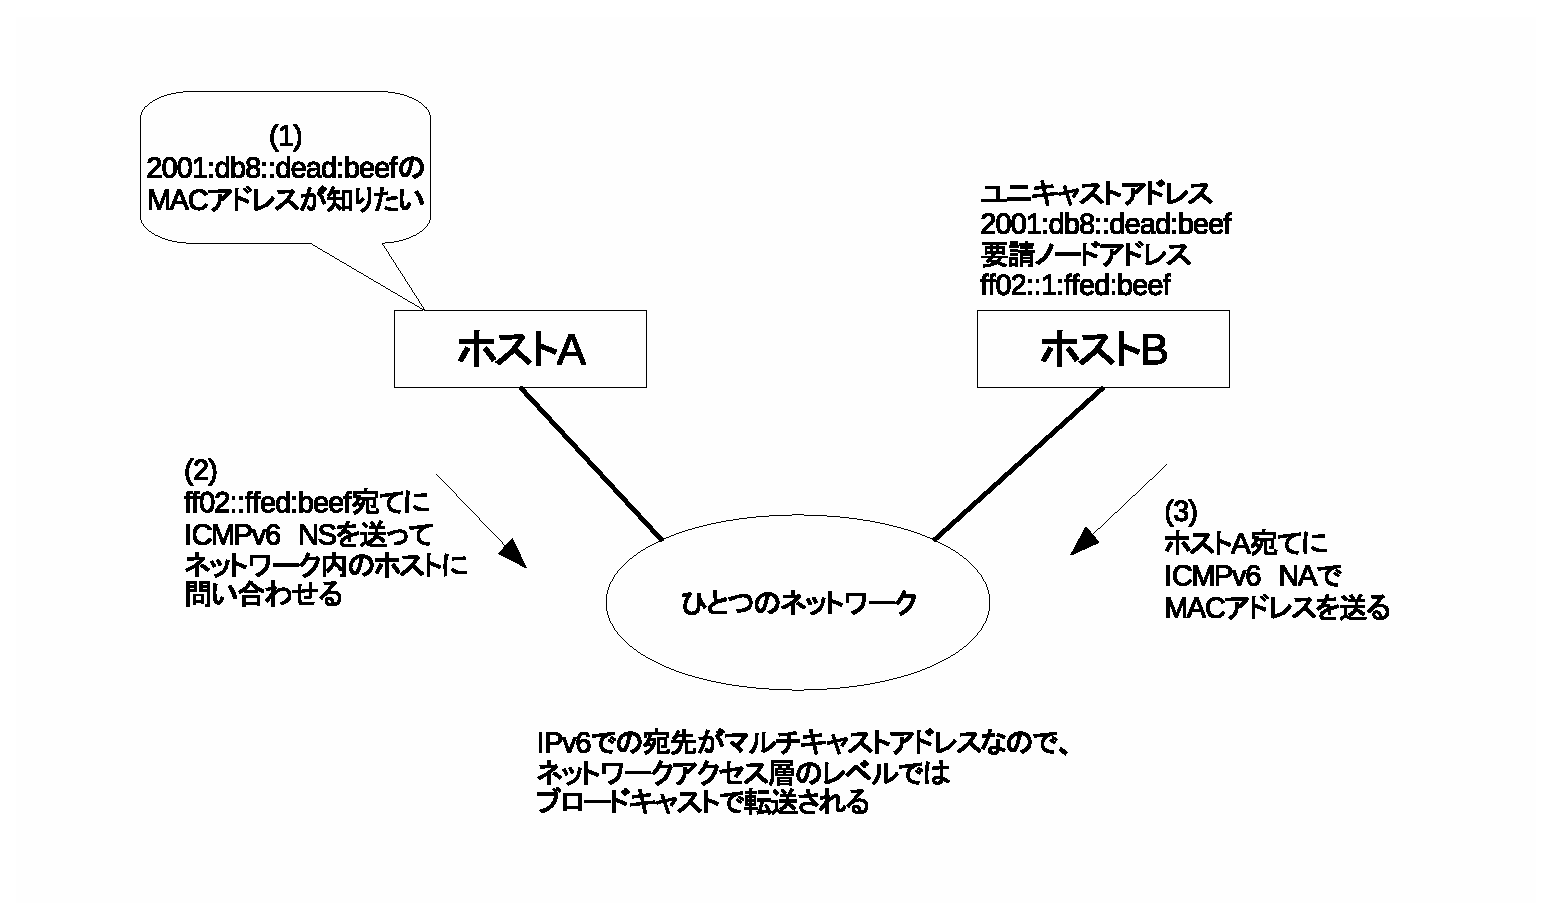
\includegraphics[width=12cm,clip]{draw/ndp.eps}
	\caption{NDPによるMACアドレス問いあわせ}
	\label{fig:NDP}
\end{figure}

ここでは、IPv6でIPv6アドレスとMACくぁドレスをマッピングするため情報収集である、NDPについて説明を行う。NDPは、Neighbor Disvocery Protocolで、近接探索プロトコルと呼ばれる。

近接探索には、ICMPv6を用いる。本稿では、その機能の一つである、IPアドレスとMACアドレスのマッピング情報の収集の説明を通じて、インターネットプロトコル層によるICMPv6の使用例を説明することを目的としたい。

NDP。IPv6アドレスやデフォルトルート情報の自動設定にも使われる。だが、本書は想定読者をネットワークアプリケーションを書くプログラマとしている。そのため、アドレス自動設定については割愛する。

前に、NDPで要請ノードアドレスを使用するという説明をした。要請ノードアドレスは、FF02::1::ff00:0000/104のマルチキャストアドレスで、下位3byteは、MACアドレスを調べたいIPv6ユニキャストアドレスのホストアドr巣部分の下位3byteと一致する。そのため、NDPを使いたい場合、ネットワークアクセス層での同じネットワークに接続できるインタフェイスは最大4096となる。


\begin{enumerate}
\item 送信側は、IPアドレスに対応したMACアドレスを探す際、自分のメモリ上にある、IPアドレスとMACアドレスの対応表を調べる。この対応表を、キャッシュに格納する。キャッシュにIPアドレスとMACアドレスの対があればそれを利用して送信する。
\item キャッシュに情報がない場合、ICMPv6で、要請ノードアドレス宛に、ICMPv6のNS(Neihbor Solicitationを)
送信する。
\item あて先の要請ノードアドレスはマルチキャストアドレスなので、ネットワークアドレス層ではブロードキャストとして配送される。
\item ネットワーク内に、該当する要請ノードアドレスを持つホストがあれば、NSを受信する
\item NSのあて先となったホストは、ICMPv6のNA(Neighbor Advertisement)でMACアドレスを回答する。
\item 問い合わせ側はその結果を利用すると共に、一定時間キャッシュとして再利用する。
\end{enumerate}

このように、 ICPMb6を用いることで、MACアドレスの解決も、インターネットプロ取る層の機能だけで実現している。

\subsection{ARPによるIPv4アドレスとMACアドレスのマッピング}

IPv4の通信路として、イーサネットのような共用伝送媒体を使用するネットワークを使うとき、IPアドレスとネットワークアクセス層のアドレスのマッピングはどのように行っているのだろうか。

それには、ARP(Address Resolution Protocol)というプロトコルを使用して、IPアドレスと物理的なホストの識別のマッピングを行う。このマッピングは、必要になったときに自動的に行われる。

以下、イーサネットにおけるARPの手順を説明する。イーサネット以外でも基本的な手順は同じである。

\begin{enumerate}
\item 送信側は、IPアドレスに対応したMACアドレスを探す際、自分のメモリ上にある、IPアドレスとMACアドレスの対応表を調べる。この対応表を、ARP テーブルと呼び、動的に生成される。ここにIPアドレスとMACアドレスの対があればそれを利用して送信する。
\item ARPテーブルに情報がない場合、ネットワークアクセス層のプロトコルで、問い合わせを乗せたフレームをブロードキャストする。これをARP要求という。
\item ARP要求はブロードキャストで行われるので、同一ネットワーク内の全てのネットワークインタフェイスが受信する。もし、問い合わせに該当するIPアドレスが割り当てられているネットワークインタフェイスがあれば、それに応答する。これがARP応答である。
\item 問い合わせ側はその結果を利用すると共に、ARPテーブルに蓄積して、一定時間キャッシュとして利用する。
\end{enumerate}

ARPは、前述の通り、共有伝送媒体を使用する、つまり、ネットワークアクセス層において、物理的なハードウエアを区別する手段があるネットワークに対して用いられる。PPPのように、ネットワークインタフェイスを一対一で接続するネットワークアクセス層では、物理的なインタフェイスを区別する必要がない。そのため、ARPを用いる必要がない。

\begin{figure}[htbp]
	\includegraphics[width=12cm,clip]{draw/arp.eps}
	\caption{ARP要求とARP応答}
	\label{fig:arp}
\end{figure}

ここで、IPv6のNDPと、ARPを比較してみよう。ARP要求もARP応答も、IPv4はネットワークアクセス層の情報を取得するのに、ネットワークアクセス層のサービスを直接駆動している。通信路としてのサービス以上ことをネットワークアクセス層に対して要求している。

後に現れたNDPのように、インターネットプロトコル層の機能で完結し、ネットワークアクセス層はあくまでも経路としてのみ使うものとは本質的に異なる。だが、この知見が後のNDPにつながったと考えるべきであろう。


\section{パケットの寿命}

データグラムは、ネットワーク間を転送されることで、いつかは宛先にたどり着く。だが、途中のルータで転送先が間違っていたなどの理由で、宛先にたどり着かないまま転送され続ける、いわば迷子になったデータグラムも生ずる。

そのようなデータグラムは、どこかで消さないとネットワークのトラフィックを永久的に圧迫してしまう。そこで、IPv4ヘッダにはTTL(Time To Life)というフィールドを置いている。このTTLで、パケットがルータを通過できる残り回数をカウントする。

IPv6では、TTLでなくホップリミットというフィールド名となる。TTLが実際には時間でなくルータを通過した回数を数えるフィールドになったことから、わかりやすい名前に改められた。

パケットが送信されるとき、TTLもしくはホップリミットには、通常は64が設定される。この数値はルータを通過する毎に1ずつ減り、0になった時点でデータグラムは破棄される。これによって、迷子になったデータグラムがインターネットの上を回り続けることを回避している。

\subsection{寿命をわざと短くしたデータグラム}

HDDのビデオレコーダでは、LAN内に録画した番組を配信できるものがある。だが、この配信は、ルータを越えることができない実装が多い、つまり、インターネット経由でアクセスできないようになっている。これは、データグラムのTTLを1にすることで、そのビデオレコーダに一番近いルータがデータグラムを破棄するように細工がしてあるためである。

\section{フラグメントとゲートウェイ}

インターネットプロトコル層が、あるネットワークアクセス層から上がってきたデータグラムを、他のネットワークアクセス層に転送する場合を考えよう。

この二つのネットワークアクセス層が同じ規格であれば、単純に、データグラムを転送先のネットワークのフレームにして送信すればよい。だが、転送先のネットワークアクセス層の規格が異なる場合はどうであろうか。転送先のフレームのデータ部分が、最大サイズが現在のデータグラムよりも小さかった場合、インターネットプロトコル層では何をしなければならないか。

それは、転送先のネットワークアクセス層のフレームに乗せることができるデータの大きさにあわせて、データグラムのサイズを変更することである。具体的には、データグラムの大きさが、転送先ののネットワークで扱えるデータの大きさになるように、データグラムのデータ部分を分割する。分割によって生じたデータクラムにも、新しくIPヘッダをつける。それによって、元が一つのデータグラムであったものを、よりサイズの小さい、複数のデータグラムとして送信し直す。

また、インターネットプロトコル層から見て、上位のプロトコルからストリームとして渡されたデータも、ネットワークアクセス層で扱えるサイズになるよう分割し、その断片の全てにIPヘッダをつける。

この動作をフラグメントという。フラグメントするときのデータ量の単位となる、ネットワークアクセス層におけるデータ部分のの大きさをMTU(Maximum Transmission Unit 最大転送単位)という。MTUは、ネットワークアクセス層のフレームの大きさではないことに注意してほしい。

インターネットプロトコル層は、ヘッダとデータの断片一つの大きさを合計したものがMTU以下になるよう、データを分割する役目ももっている。

このように、異なるMTUを持つ、つまりネットワークアクセス層の構成・構造が異なるネットワークの間で中継を行うIP層の機器を、ルータと区別してゲートウェイト呼ぶことがある。

IPv6では、経路のMTUは、ICMPv6を用いて調べることができるようになった。この手順を、PMTUや、Path MTU Discoveryと呼ぶ。PMTUは、RFC1191で定義されている。

\subsection{フラグメントのタイミング}
インターネットプロトコル層のフラグメントは、どのタイミングで行われるのだろうか。これ派、IPv4とIPv6とで、行うことが許されるタイミングが異なる。

IPv4では、あるルータが、直接転送する先への送信でフラグメントが必要であれば、フラグメントを行って送信する。これは、パケットを中継するすべてのルータが、必要であればフラグメントを行う、といことである。MTUは、直接転送する先のルータまでの経路で図られる。

一方のIPv6は、インターネットプロトコル層ではフラグメントを行わない。もし、直接通信するルータまでの経路のMTUよりも大きなパケットが到着したら、それを破棄してICMPv6で通知する。


通信の始点だけが、フラグメントを行う。送信の前にあて先までの経路のMTUを調べ、それにあわせて送信する。これは、現代では、インターネット接続に使われる経路が、パケットの転送中にかわる、つまりパケット転送中に、経路のMTUが変化することはほぼないことから、実装をシンプルにするための仕様である。

そのため、IPv6は、最初に、経路ののPMTUディスカバリを実行し、経路の最小MTUサイズを求める。そして、途中でフラグメントが必要ないMTUを設定し、データを送信する。また、フラグメントが発生した場合は、ネクストヘッダ番号41のIPv6-Fragヘッダを付加して、それぞれのフラグメントを送信する。受信側は、そのフラグメントヘッダの情報から、元のデータグラムを再構築する。


\subsection{中継先のネットワークのMTUの方が大きいときは?}

インターネットプロトコル層が、データグラムの大きさよりもMTUの小さいネットワークにデータを転送するときはフラグメント処理を行う。では、転送する先のネットワークアクセス層のMTUが、フラグメントした後のデータグラムよりも大きい場合はどうするのだろうか。

この場合はなにもしない。つまり、フラグメントを収集してデータグラムを再構築する、という処理は行われない。。理由としては、フラグメントの再構築を行うには、分割された全てのデータグラムを収集する必要がある。だが、ここまでで説明した通り、インターネットプロトコル層の性質として、全てのフラグメントが再構築を行おうとするインターネットプロトコル層を経由する保証がないことを思い出してほしい。

そのため、インターネットプロトコル層は、転送先となるネットワークアクセス層のMTUが、現在のデータグラムのサイズより小さいときのフラグメント処理しか行わない。

\subsection{フラグメントされたデータの再構築}

自分が宛先であるデータグラムを受信したときに、インターネットプロトコル層は、元のデータを構成するフラグメントを全て蓄積し、データを再構築して、ストリームとして上位プロトコルに渡す。もしこのフラグメントが一定時間内にそろわなければ、タイムアウトとして、収集したフラグメントを全て破棄する。

フラグメントされたデータを元のストリームに戻すために、インターネットプロトコル層は、IPヘッダの識別子と、フラグメントオフセットのフィールドに記載された情報を用いる。

断片がそろわずにデータグラムが破棄された場合、インターネットプロトコル層は発信元にフラグメント破棄の通知を行わない。これはデータグラム破棄の通知として、ICMPを用いて行われる。

\subsection*{}
\begin{itembox}[l]{いもうとコラム インターネット物理モデル}


実は、インターネットプロトコルの動作を見ることができる場所があります。お台場\footnote{実際の住所は江東区青海 http://www.miraikan.jst.go.jp/}にある日本科学未来館に、インターネット物理モデルという、IP層まの動作を再現したモデルが展示されています。

インターネット物理モデルは、白と黒のボールをビットとして使用し、それを端末である操作台の溝の上にならべます。それによって宛先IPアドレスとデータからなるパケットができるわけです。

次に、送信レバー(!)を引くと、パケットである、一列に並べられたボールがルータに送り込まれます。

そのルータはボールの列のヘッダであるIPアドレスを識別して、宛先となる端末と繋がっているルータに送り込みます。そして、IPアドレスに対応する宛先がない場合は、そのデータグラムはエクスパイアされます。早く言えば、ルータの下にあるかごにボールが捨てられるわけです。

図\ref{fig:miraikan}は、インターネット物理モデルの写真でする。左側にあるのが操作台で、右側の機械(ルータ)と、レールで接続されています。
\end{itembox}


\begin{figure}[htbp]
	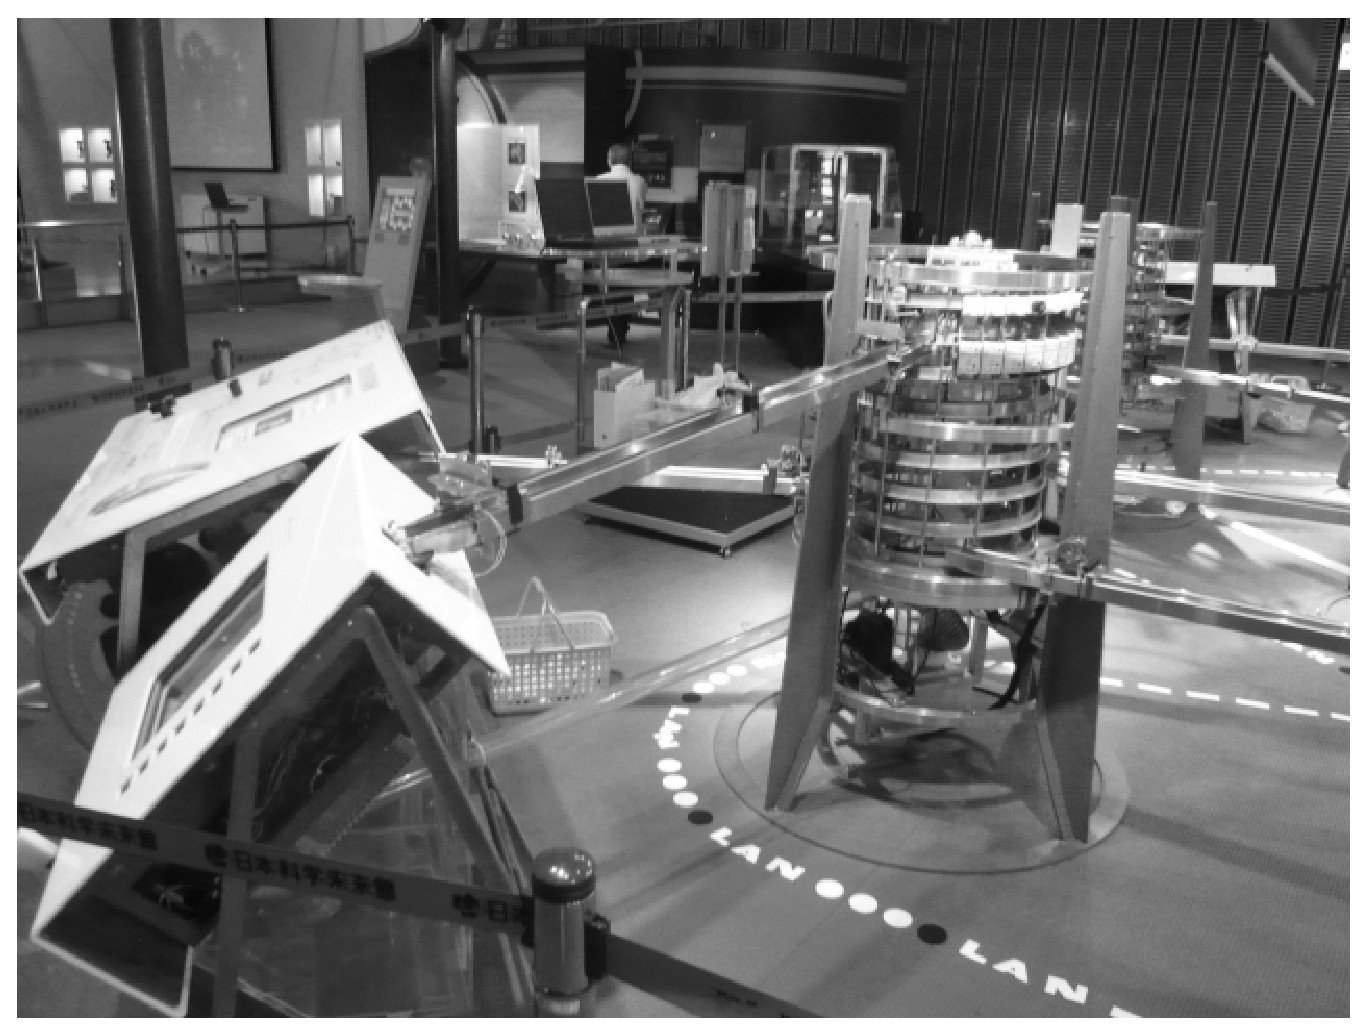
\includegraphics[width=12cm,clip]{draw/miraikan.eps}
	\caption{インターネット物理モデル}
	\label{fig:miraikan}
\end{figure}


\chapter{トランスポート層(その1) トランスポート層の概論}

アプリケーション層にサービスをするのが、トランスポート層です。トランスポート層は、ここまでで確実な通信を提供するのが役目という説明をしました。では、どうやって確実な通信をしているのか、そして、確実な通信をしなくていいときはどうしているおか、それを見てみることにします。

\section{トランスポート層とはなにか}

トランスポート層は、TCP/IPにおいて、アプリケーション層とインターネットプロと固陋そうに挟まれたレイヤである。その位置でわかるように、インターネット層のサービスを通信路として利用するレイヤである。そして、アプリケーション層にサービスを提供するレイヤである。

\subsection{トランスポート層の通信相手}
まず、トランスポートスの通信相手はなんだろうか。それは、通信の相手となるホストの上で動いているトランスポート層である。他のホスト場のトランスポート層と通信を行うことで、アプリケーションに通信というサービスを提供する。

そして、トランスポート層は、同じプロトコルのトランスポート層としか通信しない。たとえば、トランスポート層が、他のホストのアプリケーションやインターネットプロトコル層と通信をすることはないし。また、TCPとUDPが通信をすることもない。

\subsection{トランスポート層が提供するサービス}

トランスポート層とはどんなレイヤであるかを考えてみよう。ごく簡単に言えば、下位のレイヤであるインターネットプロトコル層の機能を用いて、上位のレイヤであるアプリケーション層に、通信を経路を提供する役割を持ったレイヤである。

まず、この章でアプリケーションという言葉を使うときは、特に明記しない場合、トランスポート層のサービスを利用して通信をする、TCP/IPでのアプリケーション層を指す。

たとえば、メールとWebのアプリケーションが同一ホストで動いていたとして、メールのための通信はメールのアプリケーションに、Webのための通信は、Webのアプリケーションに届ける。このように、同一ホストで動くアプリケーションは、それに割り当てられたポート番号をもちいて区別される。

それによって、ひとつのネットワークインタフェイスを、いくつものアプリケーションで使い分けることができる。つまり、ネットワークインタフェイスを多重化する。

アプリケーションから見たトランスポート層の動作とは、ネットワークのどこかにあるホストの上で稼働しているアプリケーションに、メッセージを届けることである。

トランスポート層には、それを利用するアプリケーションと、通信相手となるアプリケーションとの間に、「確実な通信」を提供するプロトコルもある。だが、確実な通信の提供はトランスポート層という概念では本質的な機能ではない。あくまでも、提供されるオプションのひとつである。だが、そのオプションこそがインターネット上のプロセス間通信にとって重要であることも忘れてはならない。

もう一つ、トランスポート層には、ある通信がどのアプリケーション宛ての通信かを判別し、該当するアプリケーションにデータを届けるという役割を持つ。

あるホストの上では、複数のアプリケーションが動作している。つまり、アプリケーション層に相当するプロセスが複数存在するということである。それぞれ名ぷりケーションごとに、到着した通信を振り分けるのも、トランスポート層の役目である。


\subsection{トランスポート層が使うサービス}

トランスポート層は、サービスとしてインターネットプロトコル層を利用する。つまり、通信相手のトランスポート層との通信経路として、インターネットプロトコル層を使用するということだ。

ここまでに説明したインターネットプロトコル層とICMPを使って、ネットワークを経由した二つの端末が通信を行うことは可能である。だが、ここでその通信とはどんなものだったかを思い出してみよう。

インターネットプロトコル層での通信とは、途中経路にあたる機器の善意を信じ、データグラムが宛先に届くことを期待する、というものであった。つまり、確実に届ける機能が備わっていない。では、インターネットプロトコル層の機能を使ってデータを確実に届けるには、どのようにすればよいのだろうか。

その、「確実に届ける」役割を担当するのがトランスポート層である。

\subsection{TCPとUDP}
本書では、トランスポート層のプロトコルとして、TCPとUDPという二つの代表的なプロコルについて説明をする。

TCP(Transmission Control Protocol)は、アプリケーションに、「確実な通信」を提供する。この確実な通信とは、送ったデータが必ず相手に届くこと、そして、データの送信順が保証されることである。送信順が保証されるというのは、順序を表す番号を付けてデータを送信すれば、到着側でその順番にデータを受け取ることができるとができる。それによって、一連のデータ、つまりストリームを送信することが可能となる。

もうひとつのUDP(User Datagram Protocol)は、ポート番号によるアプリケーションの区別、つまり、インターネットプロトコル層以下の経路をアプリケーションごとに多重化する役割のみを持つ。TCPのような確実な通信は提供しない。つまり、UDPによってアプリケーション層にトドけらルデータの、到着のしかたの性質は、インターネットプロットプロトコル層と同じである。

\subsection{ストリームとデータグラム}
アプリケーションが、トランスポート層のサービスとしてTCPをもちいて送受信するデータを、TCPストリーム、あるいは単に、ストリームと呼ぶことがある。これは、相手への到着と、データの順番が保証されるTCPによって、データが順序正しく送出されるためである。

一方、アプリケーションがトランスポート層のサービスとしてUDPを用いたとき、送受信するデータをUDPデータグラムと呼ぶ・これは、インターネットプロトコルにおけるデータグラムと同じ性質を持ったデータとなるためである。また、UDPの場合は、インターネット層のデータであるIPデータグラムと区別するために、UDPデータグラムと呼ぶ。

\subsection{コネクションとコネクションレス}
さて、ストリーム型の通信を行うための通信路の条件とは何であろうか。それは、送信側から受信側まで、一本の通信路が存在することである。このような通信路が存在していれば、切れ目ない、ストリーム型のデータを流すことができるだろう。このような通信路を、コネクション型という。

TCPは、端から端まで一本の通信路をつくり、その上でストリーム型の通信を行うプロトコル、ということもできる。

一方、コネクションを作らない通信もある。データを細切れにして、そのひとつひとつに宛先をつけてやる。そして、途中でその宛先を見て適切な転送を行う。そんな通信のやり方もある。このような通信を、コネクションを作らないことから、コネクションレス型という。

UDPは、コネクションレス型の通信をアプリケーション層が利用するためのプロtコルであると考えることもできるだろう。

\subsection{UDPの優位性}

TCPの機能を実現するためは、、コンピュータのリソースに対する負荷\footnote{TCP/IPが成立した年代のコンピュータの処理能力を基準として考えてほしい。}と、送信するデータ以外にやり取りするビット列が多いであろうことは想像に難くない。

そのため、確実性がそれほど必要でない場合、受信したという情報を待つ時間がロスになる場合、送りたいデータに比べてこのような制御情報の方がはるかに多い場合など、トランスポート層の機能がかえってじゃまになる場合がある。その場合に、UDPが優位となる。

また、近年は、インターネットプロトコル層ほぼそのままの性質を利用して、アプリケーション側でフロー制御などを実装する場合がある。既存のトランスポート層のプロトコルとは異なる機能をアプリケーションとして実装するわけである。その様な場合にも、UDPは用いられる。

\subsection{トランスポート層はどう区別されるのか}

では、インターネットプロトコル層は、トランスポート層をどのように区別するのだろうか。インターネットプロトコル層がIPv4かIPv6かで異なるが、プロトコルごとに番号を付け、それをインターネットプロトコル層が、何のデータを運んでいるのかという情報として持つ。


\subsubsection{IPv4}

IPv4では、プロトコル番号という番号割り当てられている。その番号によって、インターネットプロトコル層は、どのトランスポート層のプロトコルにデータを届けるかを区別する。

ただし、プロトコル番号は、トランスポート層のための概念ではない。インターネットプロトコル層は、トランスポート層に対してサービスを行う。だが、トランスポート層専用のその材ではない。インターネットの通信に必要なデータを他のネットワークに運ぶという役目から、インターネットプロトコル層はトランスポート層以外のデータも運ぶ。それについては改めてインターネットプロトコル層の項目で説明を行うことにしよう。

\subsubsection{IPv6}

IPv6では、プロトコル番号に相当する概念は、ネクストヘッダ番号と呼ばれるデータになる。IPv6のデータグラムのデータ部分は、トランスポート層のデータがアプリケーション層のデータをカプセル化したものが乗っているイメージとなる。

これをビット列で考えると、IPv6のヘッダの後に、トランスポート層のヘッダが並んでいる構造となることが予想される。\footnote{実際には、別の制御ヘッダがいくつか続いた後にトランスポート層のヘッダがくる場合もある。}そのため、ネクストヘッダ番号、というデータで、IPv6のヘッダの後に来るヘッダがどのトランスポート層のプロトコルかをこれで判別する。

ネクストヘッダ番号については、インターネットプロトコル層の項目で改めて説明する。

\section{トランスポート層の機能}

トランスポート層が提供する機能そてして、ここまでで、上位のアプリケーション層をに対する通信経路として説明を行ってきた。では、そのための機能にはどのようなものがあるか、本省ではそれを概論的にまとめてみたい。

\subsection{アプリケーションを特定する}

\begin{figure}[htbp]
	\includegraphics[width=12cm,clip]{draw/portnumber.eps}
	\caption{ポート番号によるアプリケーションの区別}
	\label{fig:pseudo6}
\end{figure}

トランスポート層の役割のひとつは、受信したデータを渡すアプリケーションを特定し、そのアプリケーションにデータを渡す、ということである。では、このアプリケーションの特定は、アプリケーションに割り当てたポート番号が、トランスポーつぉうのヘッダ情報として付加されている。トランスポート層は、その情報を使って、どのアプリケーションにそのデータを渡すかを決める。

ポート番号は、どのトランスポー層のプロトコルでも実装されている機能である。つまり、TCPもUDPも、そのほかトランスポート層のプロトコルは、ポート番号によるアプリケーションの区別を行う。

\subsection{データの検証}
トランスポート層は、チェックサムによって到着したデータが正しいかをチェックする。その計算には、疑似ヘッダと呼ばれる、IPアドレスとデータ長からなる、チェックサム計算用の仮想ヘッダを用いる。

この疑似ヘッダについては、後ほど改めて説明を行う。

データの検証については、インターネットプロトコル層がIPV4かIPv6かで、要件が若干異なる。IPv4のときは、UDPはチェックサムによるデータの検証を省略することも許容されていた。それは、IPv4はデータグラムのチェックサムを用いたビット化けの検証機能があり、そちらで検証されていればUDPでの検証を省略してもかまわない規約だからだ。

一方、IPv6では、インターネットプロトコル層ではデータの検証をが省略されている。そのため、TCP、UDPとも、疑似ヘッダを用いたチェックサム計算によるデータの検証が必須となっている。

\subsection{データの到着確認}

データの到着確認は、トランスポート層のプロトコルのひとつであるTCPの機能となる。

まず、確実にデータが到着した、という状況が何であるかを定義しよう。確実にデータが届いた、という状況は、送信側が、受信側がデータを受信したことを知ることができた場合であるとする。では、データを送信した側が、そのデータが受信されたことを知るにはどうすればよいのだろうか。

そのためには、データを受信した側が、受信できたという情報を、データ送信側に送ればよい。その受信できたという情報を、データグラムの送信側が受信することで、送信したデータが受信されたことを知ることができる。一定時間内に、受信できたという情報が届かなければ、送信側は同じデータを再度送信する。

ここで注意する必要があるのは、受信できたという情報も、インターネットプロトコル層を利用してデータの送信側に送られるということである。つまり、この受信できたという情報も、相手に届く保証はない。では、受信できたという情報が、データの送信側に届かなかった場合はどうなるか。データの送信側からは、送ったデータが到着しないため、相手からの受信できたという情報が来ないのか、相手側にデータが到着したのに、その相手が送信した、受信できたという情報が届かないのかの区別をすることはできない。そのため、どちらの場合でも、送信側は、受信できたという情報が届かなかったデータを、再度送信する。

ここまで説明した受信できたという情報を、確認応答(ACK Acknowledgement)という。

\subsection{フロー制御}

一度に送出するデータの量を制御することを、フロー制御という。フロー制御も、TCPの機能のひとつである。

トランスポート層でやりとりされるデータの大きさは、受信する側のトランスポート層が、どれだけの大きさのデータを受信できるかによって決定される。この、通信相手のトランスポート層の都合で決まる、データの送出単位を、セグメントと呼ぶ。上位のアプリケーション層から渡されたストリームを、セグメントに分割するのはトランスポート層の役割である。

さらに、確実な通信のためには、受信側が処理可能な範囲でデータを送信する、フロー制御を行う。これによって、到着したデータが相手に受信してもらえるようにする。このように、トランスポート層には、受信側の状況に合わせてデータを送信する機能もある。

下位のインターネットプロトコル層では、データグラムの到着順は保証されない。そのため、確実な通信のためには、データが順番通りに到着した方が都合がよい。そのために、アプリケーション層から渡されたストリームをセグメントに分割する際に、順番通りに番号を付ける。受信側は、その番号の何番まで受信したかという情報を送信側に返す。送信側はその番号を見て、届かなかったと推測されるデータを再送する。これによって、上位のアプリケーションに、ストリームの送受信をサービスする。


\subsection{コネクションの確立と切断}

TCPの通信には、明確な始まりと終わりとがある。そのため、コネクションの確立と切断、という概念が存在する。

確実な通信を行うためには、通信相手となるアプリケーションを特定し、送信者と受信者の対によって特定できる、一対一の通信を行なわなければならない。そのために、通信相手に向けて、これから通信を始めたいというセグメントを投げる。送信を始めたいというセグメントを受けとった側は、通信可能であれば通信を行う準備をして、確認応答を返す。この手順によって、通信を始める側から見た通信の相手が、今後送信するセグメントを受け取れる状態にある事を確認する。この手順をコネクションを確立するという

また、コネクションを確立するときに、一度に受信可能なデータの量や、送信するデータにつける通し番号をいくつからはじめるか、などの情報を、通信する両端で交換する。

逆に、通信を終了するときは、今後送信するデータはないという情報のセグメントを送信する。今後送信するデータはないという情報のセグメントを受信した側は、それに対して確認応答を返す。通信両端が、お互いに今後送信するデータはないという情報のセグメントを送り、それに対しての確認応答がお互いからあれば、それは、双方とも今後送信するデータはない状態となる。つまり、通信が終了する。この手順を、コネクションを切断するという。

このように、通信相手が通信可能な状況にあることを確認し、通信を行うときのお互いの情報を交換し、通信の終了を確認する。これも、トランスポート層の役割である。

\subsection*{}
\begin{itembox}[l]{いもうとコラム バーチャルサーキット}

古い解説書や教科書では、トランスポート層のコネクション確立の動作を、コネクションレスな通信路においてバーチャルサーキットを開設する、と説明していることがあります。これは、電話交換網と対比しての表現です。

電話は、回線交換によって、物理的にエンドツーエンドで通信路が設定されます。それと比較して、仮想的な通信路、つまりバーチャルサーキットが開設された、と表現していたわけです。

現在では、バーチャルサーキットという表現はあまり使われなくなっています。

\end{itembox}



\section{疑似ヘッダ}

トランスポート層は、送信元や宛先について、IPアドレスの情報を持っていない。これはある意味当然のことで、IPアドレスを用いた伝送は、下位のインターネットプロトコル層がサービスとして提供するものであり、トランスポート層では考慮する必要がないためだ。

だが、到着したデータの正当性を検証する場合、送信元や宛先のIPアドレスの情報があった方が都合がよい。そのため、トランスポート層のデータのヘッダ部分の直前に、図\ref{fig:pseudo}および、図\ref{fig:pseudo6}の、疑似ヘッダ(Pseudo Header)という、疑似ヘッダは、インターネット層のプロトコルがIPv4かIPv6かで、構造が変化する。


送信元と宛先のIPアドレスを含んだ仮想的なデータが存在することにして、チェックサム計算を行う。\footnote{その計算の際に、UDPもしくはTCPヘッダのチェックサムフィールドは0として計算する。}

疑似ヘッダを用いる利点として、チェックサム計算に送受信のIPアドレスが含まれることで、送信元や宛先の間違いも含めて、トランスポート層でデータの正当雨声検証が可能になるということである。

逆に、疑似ヘッダを用いることで、NATやVPNなど、ネットワーク機器における送信元や宛先など、IPヘッダの書き換えが生じる場合、それはトランスポート層のチェックサムにも影響する。だが、この部分については本書の範疇を超えるので、説明を割愛する。\footnote{興味があれば、NATなどのアドレス変換に関するRFCや、各種VPNに関する技術解説を参照していただきたい。}

\subsection{IPv4の疑似ヘッダ}

\begin{figure}[htbp]
	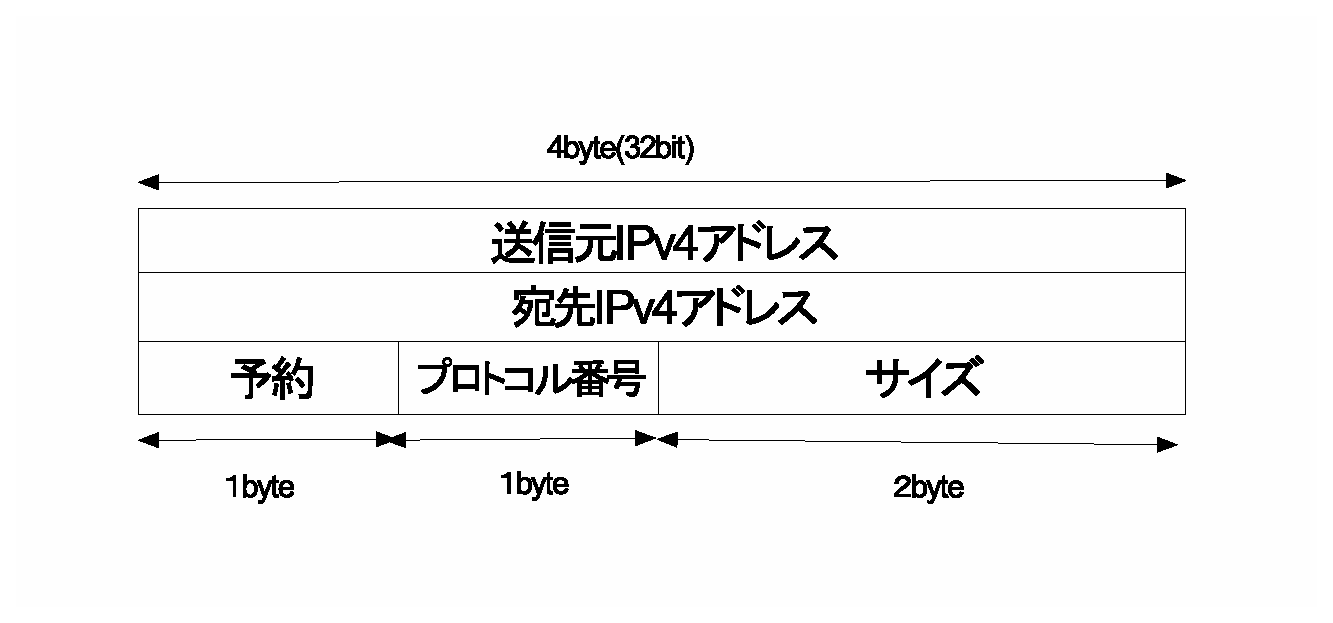
\includegraphics[width=12cm,clip]{draw/pseudoheader4.eps}
	\caption{インターネットプロトコル層がIPv4の疑似ヘッダの構造}
	\label{fig:pseudo}
\end{figure}

図\ref{fig:pseudo}は、インターネットプロトコル層がIPv4の疑似ヘッダである。

発信元IPアドレス、宛先IPアドレス、プロトコル、データ長の各フィールドで構成されている。プロトコルフィールドはTCPであれば6,UDPであれば17が入る。また、データ長フィールドには、疑似ヘッダを除く、実在するヘッダとデータ部分の長さの合計が入る。

\subsection{IPv6の疑似ヘッダ}

\begin{figure}[htbp]
	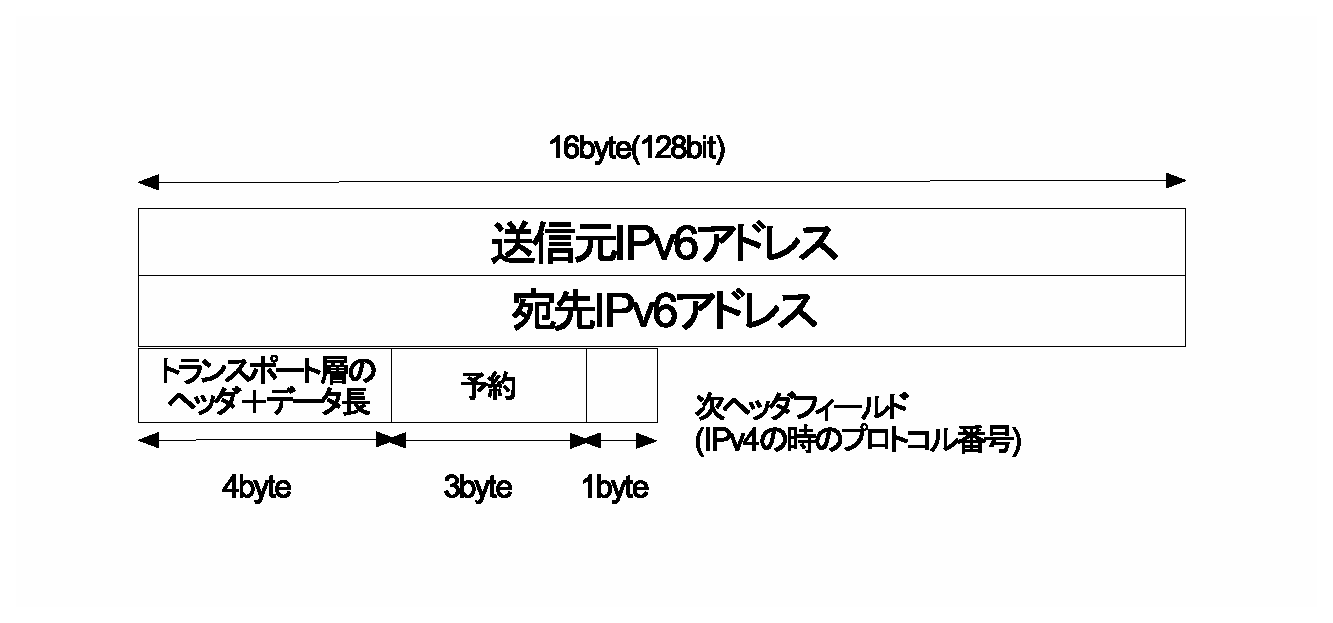
\includegraphics[width=12cm,clip]{draw/pseudoheader6.eps}
	\caption{インターネットプロトコル層がIPv6のときの疑似ヘッダの構造}
	\label{fig:pseudo6}
\end{figure}

図\ref{fig:pseudo6}は、インターネットプロトコル層がIPv6の疑似ヘッダである。

基本的な構造、内包するデータはIPv4の場合とほぼ同様である。IPv6のデータグラムは、ジャンボグラム拡張と呼ばれる拡張で、最大4GiBまでの大きさを採ることができる。そのため、サイズは32bit(4byte)となっている。予約フィールドのビットは全て0である。

また、プロトコル番号に層等するフィールドは、ネクストヘッダ番号となっている。ネクストヘッダ番号の番号自体はIPv4のプロトコル番号なので、IPv4の時と同様に、TCPなら6、UDPなら17が入る。

UDPならびにTCPでは疑似ヘッダをどう使用しているか、それぞれの章での解説で改めて説明する。


\chapter{トランスポート層(その2) UDP}

UDPは簡単なプロトコルですが、インターネットプロトコル層のパケット通信そのままです。プロトコル自体はものすごく簡単なのですが、インターネットプロトコル層の知識なしでは、理解がむずかいという落とし穴があります。

ですが、機能は簡単でも、アプリケーション層へのサービスを行うトランスポート層です。
トランスポート層プロトコルの最初の解説として、そんなUDPについて見て行くことにします。

\section{UDP}

トランスポート層の実際のプロトコルとして、ポートによる経路多重化と、疑似ヘッダによるエラーチェックだけ行うのがUDP(User Datagram Protocol)である。UDPは、データ送信の前にコネクションをはる動作がない。そのため、UDPによる通信を、コネクションレス型と言う。

また、User Datagram Protocolの名の通り、インターネットプロトコル層のデータグラムを、そのままトランスポート層経由でアプリケーションが使用できるようにしたもの、と考えることもできる。相手にデータを届けるという観点で見たUDPの基本動作は、ポートによる経路多重化が付加されただけで、インターネットプロトコル層と変わらない。

\subsection{UDPによる通信}

UDPによる通信は、通信前の準備や、データの到達確認などは行ない。オプションとして、チェックサムによるデータグラムの破損チェックがある。このように、一見すると信頼性がないプロトコルは、どのような使い方をするのだろうか。

\subsection{UDPを使うアプリケーションのプロトコル}

UDPは、エンドツーエンドのコネクションをはるコストに対して、通信の量が少ないプロトコルの場合に使用される。例えば、データグラム一つに収まる質問に対して、データグラム一つに収まる解答を返せば終了するプロトコルが該当する。
また、クライアントから送られるデータをただ記録するだけの場合にも使用される。どのような場合かというと、データの流れが基本的に一方向で、エンドツーエンドでの対話がほぼ存在しない場合などである。

前者の例として、代表的なアプリケーション層のプロトコルがDNSであり、後者の例がsyslogやSNMPである。
身も蓋もなく言えば、CPUやネットワークの貧弱であった時代に、TCPほど確実な通信でなくていいところは、通信に必要なリソースの少ないUDPで済ませていた。
また、当時の計算機やネットワークでTCPを使うとデータを取りこぼしかねなかった、重いアプリケーションが、UDPを使用していた。\footnote{そのため、近年はUDPを使用していたデータロガーをTCPを使用して実装し直す例がある。例えば、syslogの置き換えアプリとして、TCPを用いるsyslog-ngが挙げられる。}

また、IP電話や音声や動画のストリームのように、発信元に対して応答確認をする時間や、データの到着順の管理などが再生時のラグに繋がるサービスについても、UDPが使用される。もっとも、チェックサムによる破損チェックを有効にしていた場合、データの破損したUDPデータグラムは破棄される。そのため、UDPさえ使えばストリーミングは滞りなく流れるわけではない。


\subsection{UDPの実装}
ここまで説明したUDPの動作で気がついたかもしれないが、UDPの受信時の動作とは、インターネットプロトコルによって届いたデータグラムを、UDPヘッダに記載されたポート番号で特定されるアプリケーションのインタフェイスに届けることである。

また、送信時も、UDPデータグラムをIPでカプセル化して送信するだけである。トランスポート層のUDPとしての制御は全く入らない。
そのため、UDPのプロトコルスタックのコードは、IPのプロトコルスタックのコードのなかに実装されることが多い。


\section{UDPヘッダと疑似ヘッダ}

UDPは、送信元ポート、宛先ポート、データ長、チェックサムからなる、8オクテットのヘッダを持つ。
データ長のフィールドが2オクテットなので、UDPデータグラムの最大の大きさは、64KiBとなる。また、最小の大きさは、ヘッダだけの8オクテットである。

IPv4では、インターネットプロトコル層のデータの大きさが最大64KiBであり、更にネットワークアクセス層が一度に送出できるデータの大きさははそれより小さいことが多いため、最大の大きさで送信されることは少ない。

\begin{figure}[htbp]
	\includegraphics[width=12cm,clip]{draw/udpdatagram.eps}
	\caption{UDPデータグラムの構造}
	\label{fig:udpdatagram}
\end{figure}

\subsection{IPv6ジャンボグラム対応}
インターネットプロトコル層にIPv4を用いる場合、UDPでは、64KiBを越えるデータをひとつのデータグラムで送信することはできない。これは、IPv4のデータグラムのサイズの上限が、UDPのデータグラムのサイズの上限となるためである。

IPv6では、最大4GiBまでのデータをひとつのデータグラムで送信することができる。この拡張を、IPv4ジャンボグラムという。そのため、IPv6ジャンボグラムを提案したRFC2675の中で、UDPのデータサイズの拡張も定義されている。
インターネットプロトコル層にIPv6を使用しており、64kibを越えるデータを送信するときは、UDPヘッダのサイズフィールドを0にする。この値は、レガシーなUDPでは決して現れない値である。
もしサイズフィールドが0であるUDPヘッダを受信したら、到達したデータのサイズをそのUDPデータグラムのサイズとする。疑似ヘッダによるチェックサム計算には、その実際のサイズをパラメータとして、使用する。




\subsection{UDPの疑似ヘッダ}

\begin{figure}[htbp]
	\includegraphics[width=12cm,clip]{draw/udppseudoheader.eps}
	\caption{UDP疑似ヘッダを含めたUDPデータグラム}
	\label{fig:udppseudoheader}
\end{figure}


UDPは、図\ref{fig:udppseudoheader}のように、疑似ヘッダがUDPヘッダの前にあることにして、到着したデータグラムの正当性を検証する。

UDP 疑似ヘッダは、IPデータグラムのヘッダを簡略化したものである。UDP疑似ヘッダは発信元と宛先のIPアドレスの情報を含む。それによって、UDPは誤った経路で送られたデータグラムを破棄する。また、チェックサムを計算するときは、UDPデータグラムの先頭に疑似ヘッダがあるものとして計算を行う。

UDPヘッダのチェックサムフィールドの値は、疑似ヘッダ込みで計算された値となる。


算出されたチェックサムが0であれば、UDPヘッダのチェックサムフィールドは0xFFFF(1の補数演算)として送出される。これは、0に対して、1の補数を取った値となる。また、UDPヘッダのチェックサムフィールドが0x0000である場合は、送信側がチェックサムを生成しなかったということを意味する。送信側がチェックサムを生成しなかった場合、UDPはチェックサムによるデータグラムの正当性検査を行わない。

UDPでは、インターネットプロトコル層にIPv4を用い、上位プロトコルで、データ破損が問題とならない場合や、デバッグ中などは、チェックサム生成とチェックサムによる検査を省略することが許されている。これは、IPv4に、チェックサムによるデータの検証機能があることによる。

一方、インターネットプロトコル層にIPv6を用いるときは、チェックサムによる検証が必須となる。これは、IPv6では、データグラムの検証が省略されたからとなる。IPv6では、データの検証はトランスポート層のサービスとして定義された。



\subsection*{}
\begin{itembox}[l]{いもうとコラム UDP-Lite}

トランスポート層のプロトコルとして、UDPを更に緩くしたUDP-Liteというプロトコルがあります。
このUDP-Liteは、音声や動画向けを想定したトランスポート層のプロトコルです。

UDPとの違いは、音声や動画データの、ビット化けなどの軽微なデータ破損は、アプリケーション層における、デコード時の補正・補完で対応することを前提としていることです。つまり、アプリケーション層でデータの復元をを行う前提で、データグラムの到達を優先させるのがUDP-Liteというプロトコルです。

UDP-Liteは、UDPヘッダでのデータ長フィールドをチェックサム適用範囲(先頭から何オクテットまでのチェックサムを取るか)に変更しています。チェックサムによるデータの検証を行うときは、チェックサム適用範囲までのデータで計算します。
つまり、UDP-Liteでは、チェックサム適用範囲外のデータが壊れていても気にしません。

UDP-Liteは、UDPのサブセットでなくUDPと全く別の、トランスポート層のプロトコルとして実装されてます。


\end{itembox}




\chapter{トランスポート層(その3) TCP}


TCP(Transport Controll Protocol)は、インターネットプロトコルスイートにおいて、アプリケーション層に対して、確実な通信を提供するためのトランスポート層プロトコルです。この確実な通信を行うために、複雑な手順を経て通信を行っています。この章では、TCPが、確実な通信のために何をしているかを説明します。

確実な通信を行うためには、データの取りこぼしを防ぐ仕組みが必要とです。それについても説明をします。本書での説明は、イメージをつかむためのごく簡単なものです。そのため、詳しく知りたい場合は、本書付録付録や参考文献を参照してくださいね。

\section{確実な通信}

TCPでは、どのようにして確実な通信を行っているのだろうか?先ほどトランスポート層の機能として簡単に説明したが、それをもう少し掘り下げてみよう。

TCPは、確実な通信を行うために、おおまかに以下のようなことを行っている。

\begin{enumerate}
\item データを受信したら、送信側に、「届いた」という連絡をする。
\item 通信の相手が通信できる状態にあることを確認しあう
\item データをどれだけ流すかは、通信相手の自己申告に従う。また、経路の状況に応じて、調整する。
\item 「届いた」という連絡がない場合は、データを送信し直す。
\item データを受信したら、送信側に、「届いた」という連絡をする
\end{enumerate}


確実な通信をおこなうために、まず、データを受信したら、送信側に、届いたという連絡を入れることにしよう。だが、TCPが使用する下位のレイヤが提供するサービス、つまりインターネットプロトコル層が提供するサービスにはそのような機能はない。そのため、インターネットプロトコル層のサービスを使って、届いたという連絡をしたり、届いたという連絡を受けたらデータの送信が成功したことを理解するのは、TCPの仕事となる。

\subsection{ストリームとセグメント}
まず、TCPのストリームとセグメントという言葉を定義しておこう。

ストリームは、アプリケーション層から渡されたデータ、あるいはアプリケーション層に渡すデータである。アプリケーション層がトランスポート層としてTCPを使用する場合は、トランスポート層以下のデータ転送単位を考慮しない。また、データをビット列と見たとき、その送信順が保存されることを期待している。

一方のセグメントは、TCPがストリームを分割して、一度に送出できるデータの大きさに切り分けたものである。セグメントが、一度に送出される、つまり、インターネットプロt凝る層に渡されるデータ量となる。

\subsection{セグメントが一つだけの場合}
\begin{wrapfigure}[22]{r}{6cm}
	\includegraphics[width=6cm, clip]{draw/tcp01n.eps}
	\caption{セグメント一つの送信と応答}
	\label{fig:tcp01}
\end{wrapfigure}

まず、TCPで通信を行っているホストAとホストBがあるとしよう。ホストAがホストBに向けて、何らかのデータをひとつだけ送信したとする。このデータが、TCPのデータの送信単位、つまりセグメントとなる。

ホストBがセグメントを受信すると、送信元であるホストAにむけて、届いたという返事を返す。ホストAは、ホストBからの、届いたという返事を受信したら、セグメントの送信に成功したことを知ることができる。つまり、一つのセグメントの送信について、確実な通信ができたということだ。

この、届いたという返事を確認応答(ACK Acknowledgement)という。ACKは、TCPヘッダのACKビットフィールドを1にした、TCPセグメントとして送信される。

\subsection{ACKが届かない場合}

セグメントもACKも、インターネットプロトコル層によって伝送される。そのため、セグメントとACK、どちらかが届かない場合もある。では、ACKが届かない場合はどのようにすればよいのだろうか。前にも説明したとおり、送信側はセグメントが届いていないのかACKが届いていないのか、判断することができない。

そこで、ACKが届かない場合は、届くことを期待していたACKに対応するセグメントを、もう一度送信する。前に送ったセグメントがホストBにとどいていなければ、送信し直した方のセグメントが受信され、ACKが帰ってくるだろう。

では、ホストBは先に送ったセグメントを受信してACKを返していたが、そのACKがホストAに届かなかった場合はどうなるだろうか。ホストBは送信し直したセグメントを受信した後に、ホストAにACKを返す。そして、重複したセグメントを破棄する。

このように、ACKが返らない場合は、ACKが返るまで、送信側はそのACKに対応するセグメントを送信し直す。つまり、TCPの確実なやり取りとは、ACKと、ACKが届かなかったときのセグメントの送信し直しで成り立っている。

\subsection{シーケンス番号と確認応答番号}
\begin{wrapfigure}[22]{r}{6cm}
	\includegraphics[width=6cm, clip]{draw/tcp02n.eps}
	\caption{シーケンス番号と確認応答}
	\label{fig:tcp02}
\end{wrapfigure}

ホストAが送信するセグメントが複数であった場合を考えよう。この場合には、セグメント一つを送信する場合にはない問題が生じる。それは、戻ってきたACKがどのセグメントに対応しているかわからないということである。

インターネットプロトコル層の特性を考えると、ホストAが送信したセグメント(をデータとして持つIPデータグラム)が、その送信順にホストBに到着する保証はない。同様に、ホストBが送出したACKが、送信した順番でホストAに到着する保証もない。さらに、セグメントのどれか、ACKのどれかが到着しない可能性もある。このとき、どのACKがどのセグメントに対してのACKかを区別するにはどのような方法があるだろうか。

どのセグメントに対するACKかを判別するために、セグメントとACKに番号を付ける。そして、セグメントの番号と、ACKの番号を対応させて、どの ACKがどのセグメントに対応しているかを判別すればよい。

セグメントに付ける番号は、シーケンス番号と呼ばれる。ここで気をつける必要があるのが、シーケンス番号はセグメントの送信順に付けられる番号ではないということだ。シーケンス番号は、そのセグメントで運ぶデータが、上位のアプリケーション層から渡されたストリームの先頭から数えて何オクテット目になるか、を示す番号である。\footnote{TCPでは、ポート番号ごとにシーケンス番号が存在する、ということである。}

説明のために例を示そう。シーケンス番号1のセグメントが、500バイトのデータを持っていたとする。すると、その次に送信されるセグメントのシーケンス番号は、501になる。ここで、シーケンス番号501のセグメントが、200バイトのデータを持っていたとしたら、その次に送信されるセグメントのシーケンス番号は、701になるであろう。

では、ACKに付けられる番号はどのように決められるのであろうか。ACKの番号とは、このACKを受信した後で、ストリームの先頭から数えて、この番号にあたるオクテットからデータを送信してほしい、という番号である。そのため、ACKの番号はシーケンス番号ではなく、確認応答番号と呼ばれる。

では、ACKにつける番号として、シーケンス番号でなく、次はここからデータを送って、という確認応答番号を使用するのはなぜだろうか。シーケンス番号をそのまま返せば、送信側はそれで確認ができるのではないだろうか。

ACKが確認応答番号を使用する理由を説明するためには、簡単にでも、送信したセグメントがどのように受信されるかを説明しなければならない。到着したセグメントのデータ部分は、受信側のバッファに入れられる。そして、シーケンス番号の順に、上位のアプリケーションに引き渡される。ここで、セグメントの到着順が前後した場合にどうなるかを考えてみよう。受信側は、まだ到着していないセグメントを受信するまで、それ以降のシーケンス番号を持ったセグメントのデータは、バッファに置かれたままとなる。このように、TCPの受信では、到着したデータが送信順にアプリケーションに引き渡されるように、バッファにデータを留め置くことがある。

確認応答番号を使用すれば、複数セグメントについてのACKを、ひとつのACKにまとめて通知をすることができる。先の例で行けば、シーケンス番号1と501の二つのセグメントが、ホストAからホストBに送信されたとする。そして、シーケンス番号501のセグメントは200バイトのデータを持っていたとしよう。このとき、受信側のホストBは、確認応答番号501と701のふたつのACKを返してもよい。また、確認応答番号701のACKを一つ返すだけでもいい。このどちらでも、送信側ホストAは、ストリームの先頭から700オクテット分のデータが受信されたことを知ることができる。

ACKでは、シーケンス番号でなく、確認応答番号を用いることで、送信しなければならないACKを減らすことができる。

\subsection{通信の相手が、通信できる状態にあることを確認しあう}
\begin{wrapfigure}[22]{r}{7cm}
	\includegraphics[width=7cm, clip]{draw/tcp04n.eps}
	\caption{3way Handshake}
	\label{fig:tcp04}
\end{wrapfigure}


TCPでは、確実な通信を行うために、通信の相手が通信できる状態にあることを確認しあう。では、TCPの説明の最初に、この手順の説明を行わなかった理由はなんだろうか。それは、TCPでは、通信の相手を確認するために、ACKを使用するためである。

ホストAからホストBに対して、TCPによる通信を開始する場合のタイムラインを追いかけてみよう。

まず、ホストAは、SYNという、これから通信を開始したい、という意味を持つセグメントをホストBにむけて送信する。この一番最初のセグメントは、UDP同様、無手順で送信される。このSYNは、TCPヘッダのSYNビットフィールドを1にした、データ部分のないセグメントである。また、SYNには、ISN(Initial Sequende Number)とMSS(Maximum Segment Size)という二つの情報が付加されている。SYNの持つこの二つの情報は何を表すのだろうか。



ISNは、ここまでで説明したシーケンス番号を、今後の通信で何番から始めるか、という値である。シーケンス番号は無符号32bit整数であり、セキュリティ上ランダムな番号をISNとすることが多い。つまり、シーケンス番号は1から始まるとは限らない。むしろ、1から始まることの方が珍しい。

MSSは、その名の通り、送信を期待するセグメントの大きさの上限である。経路のインターネットプロトコル層でフラグメントされないであろう大きさが設定される。

SYNを受け取った側は、そのSYNに対してACKを返す。ここで、ACKの返す確認応答番号は、SYNについていたISNに1を加えたものとなる。SYN はデータ部分を持たない。それなのに、なぜシーケンス番号を消費するのか。それは、ACKが送信されるときは、それが応答するするセグメントのシーケンス番号より大きい番号を、次にここから送信しろという意味で確認応答番号とする、というルールに例外をつけないため、と思えばよいだろう。

次に、ホストBは、ホストAにむけてSYNを送る。このとき、ホストB側のISNとMSSの情報を、SYNに乗せる。

このホストBから続けて送られるACKとSYNは、通常は分けて送らない。同じTCPのヘッダで、SYNとACKの両方のフラグを立てて送信する。そのため、ホストBから、応答としてSYNACKを返す、という表現をする。

SYNACKは、TCPヘッダのSYNビットフィールドとACKビットフィールドが1であり、シーケンス番号のフィールドにISN、確認応答番号のフィールドに、ホストAのSYNのISNに対する確認応答番号番号が入った、TCPセグメントとなる。

最後にホストAが、ホストBからのSYNに対するACKを返す。これで、お互いに通信ができる状態にあることを確認する手続きが完了した。ここまで完了したとき、ホストAとホストBの間で、コネクションが確立した、という。

コネクションが確立したときに、最初にSYNを送信した側をアクティブオープン、それに応答してSYNACKを返した側を、パッシブオープンという。

また、コネクションが確立するまで、ホストAからBへ(SYN)、ホストBからAへ(SYNACK)、ホストAからBへ(ACK)と、3回、セグメントが送受信される。そのため、TCPのコネクション確立を、3way Handshakeという。

TCPのコネクション確立に限ったことではないが、中央集権的な「交換機」に相当するものがないネットワークでは、全てのエンドは対等な地位にある。コネクションは、通信を行うこと必要になったエンドが、通信相手にコネクションの開設を要求することで行われる。この、コネクションを要求する側をイニシエイター、良い宇窮される側をターゲットと呼ぶことがある。\footnote{SANの一種であるiSCSIも、イニシエイター、ターゲットという用語を用いる。}


\subsection{通信を切断する}
コネクションを確立する手順が存在したのだから、コネクションを切断する手順も存在する。

まず、何をもってコネクション切断というのかを定義しよう。それは、通信を行っている双方が、相手からこれ以上送信されるデータはないという事を確認しあった状態であるとする。

\begin{wrapfigure}[21]{r}{7cm}
	\includegraphics[width=7cm, clip]{draw/tcp05n.eps}
	\caption{コネクション切断}
	\label{fig:tcp05}
\end{wrapfigure}

例として、ホストAとホストBがコネクションを確立し、通信していたとしよう。ここで、ホストAからの、全てのデータの送信が終了したとする。このとき、ホストAは、ホストBにむかって、FINというセグメントを送信する。FINは、TCPヘッダのFINビットフィールドが1 であり、シーケンス番号を持つTCPセグメントである。このホストAからのFINを受信したホストBは、そのFINに対してのACKを返す。

だが、このホストBが出すACKは、ホストBからのFINに乗せる、いわばFINACKとして送信されることはない。それはなぜだろう。

それは、ホストAからFINが到着した時点では、ホストAから送信されるデータはもうないという意味であり、即時のコネクション切断を求めるという意味ではないためである。そのため。ホストAからFINを受け取った後でも、ホストBからホストAに向けてデータを送信することが可能である。このように、通信を行っている片方からFINが来て、それにACKを返した後に、FINを送信した側へデータを送る状態を、TCPハーフクローズという。

TCPハーフクローズの状態でも、ホストBから送信されるセグメントに対して、ホストAはACKを返す。この状態では、このコネクションにおいて、ホストAからデータが送信されることがなくなっただけである。ホストAがホストBから送信されるセグメントの受信が終了したわけではない。

\begin{wrapfigure}[15]{r}{6cm}
	\includegraphics[width=6cm, clip]{draw/tcp06n.eps}
	\caption{TCPハーフクローズ}
	\label{fig:tcp06}
\end{wrapfigure}


ホストBは、データの送信が完了したら、ホストAにFINを送信する。この時点で、ホストBから送信されるデータがもうないことが、ホストAに通知された。それに対してホストAがACKを返したら、ホストA、ホストBとも、相手から来るデータはもうない、ということを知ったことになる。それ以降の通信は行われず、それをもってコネクションが切断されたということになる。


では、なぜコネクションの切断に関しては、ハーフクローズという概念が存在するのだろうか?FINに対してACKを返した時点で、コネクションが切断されてもいいのではないか、そのような疑問をもったのではないだろうか。

TCPでは、通信を行っているプロセスはそれぞれ独立して存在し、お互いを関知せずに動作している。そのため、送信が終わった、という通知も独立して行うべきであるという思想がその根底に存在する。そのために、双方が通信の終了を宣言し、双方が確認応答しないと、コネクションは切断されない。

また、リモートシェル系のアプリケーションは、ハーフクローズを積極的に使用する。rshなどのリモートシェルでは、クライアント側がシェルコマンドを送信した時点でハー風クローズし、サーバ側は実行結果をハーフクローズ状態でクライアントに返し、その後コネクションを切断する。

\subsection{遅延ACKとピギーバック(piggy back)}
\begin{wrapfigure}[22]{r}{7cm}
	\includegraphics[width=7cm, clip]{draw/tcp03n.eps}
	\caption{遅延ACKとピギーバック}
	\label{fig:tcp03}
\end{wrapfigure}

TCPでは、セグメントを受信すると、それに対してACKを返す。このACKとはどのようなものかを、改めて考えてみよう。

ACKは、TCPのヘッダにあるACKフラグを有効にし、ヘッダ内の確認応答番号のフィールドに、次に送ってほしいセグメントの番号を入れたものである。つまり、ACKも、TCPのセグメントとして送信される。

ここで、ACKをひとつ送信するコストを考えてみよう。ACKを一つ送信するのに、TCPヘッダのみの、20オクテットの大きさを持つセグメントを送信する必要がある。当然、このセグメントをインターネットプロトコルで送信するために、IPヘッダの20オクテットが追加される。つまり、ACKひとつを伝送するために、40バイトのデータをネットワークアクセス層に流さなければならない。\footnote{実際には、ネットワークアクセス層のヘッダやトレイラの分も追加される。}

これは、回線速度が遅い時代には、それなりに重い負荷であった。たかがACK一つ送信するのに、320bitものデータを流さなければならないのだ。また、ACKひとつで一つのIPデータグラムとなるので、経路にあるルータの負荷を増すし、まわりまわってACKが途中で捨てられてしまう可能性もないとは言えない。そのため、単独でACKだけを送信する状況が発生しないようにしたかった。


そこで、ACKを送信する必要が生じた場合、ACKを送信する側に、ACKを送信する先に送る、ACK以外のセグメントが発生しないか、一定時間待つ。そのようなセグメントが生じたら、ヘッダにACKの情報を便乗させる。これは、ACKの情報である確認応答番号が、TCPヘッダの中で独立したフィールドをもってしていることで可能となる。

このように、送信されるセグメントのヘッダにACKの情報も一緒に載せて送ることを、ピギーバック(piggy back)という。日本語にすると親亀子亀のスタックや、便乗という言葉をイメージすればいいだろう。

通常、ACKを送信する際は、ピギーバックできるセグメントがないか200msec待つ\footnote{規格では500msec待ってかまわない。}そして、待ち時間を過ぎてもピギーバックできるセグメントがなければ、ACKはACKだけで送信される。この、便乗できるセグメントがないまま待ち時間いっぱい待って、その後で送信されるACKを、遅延ACKと呼ぶ。

ACKは通常、ピギーバックもしくは遅延ACKとして送信される。だが、セグメントを受信した後にすぐACKを送信しなければならない場合があるため、 OSの実装毎に、遅延ACKを抑止する方法が用意されている。


\section{相手が受信できるだけデータを送る}

TCPでは、確実な通信を行うために、相手が受信できるだけのデータを送信する機能がある。

TCPでは、セグメント毎にACkを返すことになっている。だが、ACKの到着を待って次のデータを送信していたら、セグメント一つ送信するごとに、セグメントとACKで一往復となり、時間がかかる。送信すべきデータがあらかじめ存在し、その大きさがそれがMSSより大きい、つまり、複数のセグメントを送信しなければならないことが分かっている場合、それは時間がかかってしまう。

そのような場合、ACKを待たずにある程度のデータをまとめて送信してしまい、後でそれらのACKをまとめて受信すればいいのではないだろうか。TCPでは、MSSより大きいデータを送信する場合は、複数のセグメントを、ACKを待たずに送信することができる。だが、ここで一つ問題がある。ACKを待たずに、どのくらいの量のデータを送信していいのだろうか。

\subsection{受信バッファと送信量制御}

トランスポート層が受信したが、まだアプリケーション層に引き渡されていないデータを貯留する小さなメモリを、受信バッファ、もしくは単にバッファと呼ぶ。送信側が送出したデータの総量が大きすぎれば、バッファに入りきらないデータが捨てられる。それは、確実な通信の妨げになるだろう。この受信バッファとは、TCPが受信に使用する領域である。

そこで、TCPでは、受信側に、その時点で受信可能なデータの総量を自己申告してもらう、という方法をとっている。TCPヘッダには、その大きさを自己申告するためのフィールドが予約されている。そのフィールドを、ウインドウ・サイズという。

今回も、TCPの通信で、送信する側をホストA、受信する側をホストBとして説明しよう。ホストBは、ACKを返すときなど、ホストAに何らかのセグメントを送信する毎に、受信したデータを一時的に置いておくバッファの大きさがどれだけ残っているかを、TCPヘッダのウインドウ・サイズに入れて送信する。バッファの大きさを伝えることを、ウインドウ・サイズ広告という。ウインドウ・サイズは、それが広告された時点でのバッファの残りである。では、ウインドウ・サイズ分いっぱいのデータを送信しても大丈夫ということだろうか?

\begin{wrapfigure}[27]{r}{7cm}
	\includegraphics[width=7cm, clip]{draw/tcp07n.eps}
	\caption{バルク送信とウインドウサイズ広告}
	\label{fig:tcp07}
\end{wrapfigure}

ホストAが、ホストBからのウインドウサイズ広告のついたACKを受信した時点で、ホストAが送出したセグメントのうち、対応するACKが戻ってきていないものが、いくつかあったとする。そのセグメントは、これから受信バッファに取り込まれるだろうから、受信バッファを消費することになる。そこで、ウインドウ・サイズ広告から、送出したがACKが戻ってきていないセグメントの、データの総量を引く。そして残ったのが、これからACKを待たずに送信可能なデータの量となる。

では、受信側が自己申告する受信バッファの大きさを、ウインドウ・サイズというのはなぜだろうか。それは、ここまでの説明を、図にしてみることで理解することができるだろう。

まず、送信側が送信するストリームを、一直線に並べる。ここでは、説明をし易くするために、ISN=0,MSS=1として話を進めよう。送信したいデータと、シーケンス番号を一直線に並べると、以下の図のようになる。

\begin{figure}[h!] \caption{ウインドウサイズ広告(1)} \label{windowsize1}
\begin{center}
{\scriptsize
\begin{verbatim}
Stream     H  E  L  L  O sp  W  O  R  L  D sp  T  H  I  S sp  I  S sp  F  I  N  E sp  D  A  Y lf cr              
         +--+--+--+--+--+--+--+--+--+--+--+--+--+--+--+--+--+--+--+--+--+--+--+--+--+--+--+--+--+--+......
Seq #      1  2  3  4  5  6  7  8  9 10 11 12 13 14 15 16 17 18 19 20 21 22 23 24 25 26 27 28 29 30  
\end{verbatim}
}
\end{center}
\end{figure}

ここで、確認応答番号1のACKと共に、ウインドウ・サイズ5が戻ってきたとしよう。この場で一度に送信できるのは、シーケンス番号1から数えて5セグメント分である。これを図示すると、以下のようになる。

\begin{figure}[h!] \caption{ウインドウサイズ広告(2)} \label{windowsize2}
\begin{center}
{\scriptsize
\begin{verbatim}
_________|<WindowSize >|      
Stream     H  E  L  L  O sp  W  O  R  L  D sp  T  H  I  S sp  I  S sp  F  I  N  E sp  D  A  Y lf cr              
         +--+--+--+--+--+--+--+--+--+--+--+--+--+--+--+--+--+--+--+--+--+--+--+--+--+--+--+--+--+--+......
Seq #      1  2  3  4  5  6  7  8  9 10 11 12 13 14 15 16 17 18 19 20 21 22 23 24 25 26 27 28 29 30  
\end{verbatim}
}
\end{center}
\end{figure}

この図でわかるように、ウインドウ・サイズとは、送信側が送出するストリームの上に開いた、「この部分を送出する」という窓(ウインドウ)である。

では、この状態でホストAが3セグメント分のデータを送出し、ホストBからACK 3 ウインドウサイズ3が帰ってきたとしよう。

\begin{figure}[h!] \caption{ウインドウサイズ広告(3)} \label{windowsize3}
\begin{center}
{\scriptsize
\begin{verbatim}
_______________Window Size
_______________|<----->|      
Stream     H  E  L  L  O sp  W  O  R  L  D sp  T  H  I  S sp  I  S sp  F  I  N  E sp  D  A  Y lf cr              
         +--+--+--+--+--+--+--+--+--+--+--+--+--+--+--+--+--+--+--+--+--+--+--+--+--+--+--+--+--+--+......
Seq #      1  2  3  4  5  6  7  8  9 10 11 12 13 14 15 16 17 18 19 20 21 22 23 24 25 26 27 28 29 30
ACK            |<-ACK 3  
Sent           ->|
\end{verbatim}
}
\end{center}
\end{figure}

窓の左端は、受信したACKの確認応答番号で、一番大きいものに一致するシーケンス番号を持つセグメントとなる。送信したセグメントのうち、シーケンス番号が一番大きいのは3だが、戻ってきたACKの確認応答番号で一番大きいものは3である。そのため、送出したセグメントのうちシーケンス番号3は、まだ受信側のバッファに入っていないことが分かる。この状況で送出可能なデータの量は、ウインドウ・サイズの3から、送出したがまだバッファに入っていないデータの大きさ1をひいて、2となる。つまり、シーケンス番号4とシーケンス番号5の、合計二つのセグメントを送出できることが分かる。

シーケンス番号4と5のセグメントが送信された状態で、今度はACK4 ウインドウサイズ4が戻ってきたとしよう。つまり、シーケンス番号1と2に相当するデータが上位のアプリケーションに渡され、その分のバッファが空いた状態である。この状態の図を書くと、以下のようになる。

\begin{figure}[h!] \caption{ウインドウサイズ広告(4)} \label{windowsize4}
\begin{center}
{\scriptsize
\begin{verbatim}
___________________Window Size
__________________|<-------->|      
Stream     H  E  L  L  O sp  W  O  R  L  D sp  T  H  I  S sp  I  S sp  F  I  N  E sp  D  A  Y lf cr              
         +--+--+--+--+--+--+--+--+--+--+--+--+--+--+--+--+--+--+--+--+--+--+--+--+--+--+--+--+--+--+......
Seq #      1  2  3  4  5  6  7  8  9 10 11 12 13 14 15 16 17 18 19 20 21 22 23 24 25 26 27 28 29 30
ACK               |<-ACK 4  
Sent                 ->|
\end{verbatim}
}
\end{center}
\end{figure}

このように、ウインドウの左端はACKによって右方向に移動する。一方、ウインドウの右端は、バッファが空くことで、右側に移動する。ウインドウサイズが小さくなるのは、ウインドウの右端が右に動く量よりも、左端が右に動く量の方が多い場合である。また、ウインドウサイズが大きくなるのは、ウインドウの左端が右に動く量より、右端が右に動く量の方が大きい場合である。これらの動作が、引き戸の窓を左右に動かすように見える。そのため、この方法によるデータ総出量の調整を、スライディングウインドウという。

スライディングウインドウでは、窓の右端、左端とも、右に動くことはあっても左に動くことはない。また、窓の左端が、その窓の右端に追いついた状態を、ゼロウインドウと呼ぶ。ゼロウインドウのときは、いわば窓が閉じた状態であり、受信バッファに空きがないことを意味する。そのため、ゼロウインドウのときはデータを送信しない。

スライディングウインドウで注意すべきなのは、これは送信側が、受信側のウインドウ・サイズ広告と、ACKの到着状況と送出済セグメントの関係から割り出した、送信側の主観によるものであるということである。TCPにおいて、そのセグメントの送出量を制御する第三者はいない。そのため、ウインドウサイズに合わせての送信は、、送信側が自主的に行う必要がある。

\subsection{送り直しとデータの送信量の制御}

TCPでは、受信側が受信できなかったデータの再送と、送信量の制御はほぼ一体となっている。TCPの重要な機能として、最後にこれらを説明しよう。まず、ここで言う送信量とは、先度説明したスライディングウインドウではなく、途中の経路の状況に応じて調整する送信量である。

\subsection{再送信が必要な状況}

TCPで、データ(セグメント)の再送信が必要になるのはどのような状況であろうか。まずそれを見ていこう。

まず、TCPでは、セグメントが途中で失われた、もしくはセグメントが破損していたということを送信側が知るには、どのようにするのかを振り返ってみよう。TCPでは送信側は、時間内にACKが返らないということを目安に知ることができる。このとき、全てのセグメント不着の事例において、セグメントの破損は1パーセント以下の確立でしか発生しないとされる。それは、IPヘッダが破損せず、IPヘッダのチェックサムに矛盾が生じず、TCPのセグメントだけ破損するという事例はほとんど生じないためである。つまり、セグメントの不着や破損は、下位のサー^ビスが原因となって発生することのほうが、圧倒的に多い。

そのため、ACKが時間内に戻らないタイムアウトは、経路の途中で、TCPから見た下位のサービスの能力以上の通信があったために、到着していないと考えることができる。その状況で確実な通信を行うためには、相手に届かなかったと思われるセグメントを再送信すると共に、ACKを待たずに送信していたデータの量を減らす必要がある。そのため、TCPではセグメントの再送信と送信量の制御が一体になっている

\subsubsection{ACKで状況を伝え、確認する}

TCPでは、送信側に、受信側からのACKが返ったことで、それに対応するセグメントは受信されたと判断する。では、ACKを用いて、セグメントが受信されなかったことを知るにはどうすればいいだろうか。これをケース別に考えてみよう。

\subsubsection{ACKが時間内に届かなかった}

あるセグメントに対応するACKが時間内に到着しなかった場合、TCPでは、そのセグメントを再度送信しなおす。このとき、セグメントを再送信する毎に、タイムアウトの待ち時間を増加させる。

\subsubsection{重複ACKが届いた}



以下のような状況で、重複ACKという、同じ確認応答番号を持つACK画幅数回到着する現象が発生する。

\begin{wrapfigure}[27]{r}{7cm}
	\includegraphics[width=7cm, clip]{draw/tcp08n.eps}
	\caption{重複ACK}
	\label{fig:tcp08}
\end{wrapfigure}

TCPの通信において起こりうるのは、スライディングウインドウに従って、まとめて送出したセグメントのうち一部が届かない、ということである。この場合、シーケンス番号順に到着せず、順番が前後した場合と、セグメントが届かなかった場合とがある。

前者の場合、受信側は、到着したセグメントのもつシーケンス番号から、届かなかったセグメントが存在することを知ることができる。シーケンス番号の順番通りにセグメントが届かなかった場合、受信側は、届かなかったシーケンス番号を持つセグメントが到着するまで、他のセグメントが到着する毎に送出するACKの、確認応答番号を、届かなかったとおもわれるセグメントのシーケンス番号に対応するものとする。





この確認応答番号のACKは、届かなかったシーケンス番号のセグメントが到着するまで送出される。この、同じ確認応答番号をもって複数回送出されるACKを、重複ACKという。

重複ACKを受信した送信側は、その数を数える。重複数が1もしくは2(同じ確認応答番号のACKがふたつもしくは三つの場合)で、それ以降確認応答番号が、送出したセグメントに応じて増加していった場合は、シーケンス番号通りではないが、セグメントは到着したことが判る。

重複ACKの重複数が3を越えたら、つまり同じ確認応答番号のACKが4個を越えたら、それは途中でセグメントが失われたと判断する。送信側は、重複ACKの確認応答番号に対応するシーケンス番号を持つセグメントを、再送信する。

\subsection{輻輳の回避}

TCPにおける通信の送出量は、スライディングウインドウで通知される、受信側の現時点での受信能力という上限が存在する。だが、それに達していなくても、到着しなかったり順番が入れ替わったりするセグメントが発生する。それはすなわち、通信の経路がその伝送能力を超えた状態にあるのではないか、そう考えるべきであろう。通信の経路をその処理能力以上のデータが通ろうとしていて、結果、データグラムが捨てられる状況を、通信の言葉で輻輳(ふくそう)という。

ここでは、その輻輳の回避について、簡単に説明をしたい。

TCPでデータを送信する際は、最初から、受信側が通知したウインドウサイズ一杯のデータを送信するわけではない。最初は1セグメントから送信を開始し、ACKが戻る毎に、 ACKを待たずに送信するセグメントの数を増やしていく。そのように、ACKを待たず送出するセグメントの数を増やしていくと、ACKが時間内に返らなかったり重複ACKが返ったりする現象が起こる。この場合、途中の経路で輻輳が起こっている可能性がある。

ACKが時間内に返らない場合は、途中の回線がかなり輻輳していると推測できる。そのため、ACKを待たずに送信するセグメントの数を1に戻す。

重複ACKの場合は、輻輳が発生した瞬間があったが、その前後で通信は行われていた状況である。そのため、ACKを待たずに送信するセグメントの量をそれまでの半分にして、そこからまた、ACKを待たずに送出するセグメントの数を増やしていく。

この輻輳回避を行うことで、ACKを待たずに送信されるセグメントの数は、その時点の最適値の周りで振動収束する。



\subsection{タイムアウト}

\begin{wrapfigure}[20]{r}{7cm}
	\includegraphics[width=7cm, clip]{draw/tcp09n.eps}
	\caption{タイムアウト}
	\label{fig:tcp09}
\end{wrapfigure}

最後に、TCPにおけるタイムアウトについて説明しよう。ここまで何となくタイムアウトという言葉を用いてきたが、具体的に何秒待てばタイムアウトになるのか、という説明はしなかった。それは、TCPにおけるタイムアウトは、あるセグメントを送出して、それに対応したACKが戻ってくるまでの時間を評価して、決定するためである。



あるセグメント送信後、それが到達しなかったとみなして、再度おなじシーケンス番号をもつセグメントを送出するまでの時間を、再送時間(RTO Resend Time Out)という。実測値からRTOを決定するには、古典的な方法とJacobsonの提案によるものの二種類がある。現在では、実測値のばらつきを考慮してあり、整数演算かつ係数の乗除算がシフト演算で行えるJacobsonの方法が用いられることが多い。古典的な方法は、実数演算を行う必要があるため、Jacobsonの方法より演算のりソースを必要とする。

あるセグメントのタイムアウト時間は、再送を行う毎に、指数関数的に増加していく。タイムアウトは、コネクション毎でなく、セグメント毎に測定される。このタイムアウト時間の合計が、トータルタイムアウト時間、という時間に達したら、TCPは通信が不可能であると判断し、コネクションを切断する。トータルタイムアウト時間は、約9分に設定され、多くのTCPの実装で変更することはできない。そのため、アプリケーションの実装で、もっと短い時間で切断するよう実装することが多い。

\section{TCPヘッダ}

\begin{figure}[htbp]
	\includegraphics[width=12cm,clip]{draw/tcpheader.eps}
	\caption{TCPヘッダの構造}
	\label{fig:tcpheader}
\end{figure}

TCPのヘッダの構造は、図\ref{fig:tcpheader}のようになる。ここまでの説明で登場しなかったデータを収めるフィールドについて、説明をしていく。

\subsection{オプションフィールド}
TCPヘッダには、任意長のオプションフィールドがある。このオプションフィールドは、TCPの機能拡張などに用いられている。

フォーマットは、先頭から、kind、size、オプションのデータとなる。サイズフィールドは、先頭2byte(kind,size)を含んだ大きさとなる。オプションは定義されている限り、いくつ連続させてもよい。

オプションフィールドは将来拡張に用いられる。また、受信側は、未実装のオプションを受信したときはこれを無視してよい。そのため、未実装のオプションの「読み飛ばし」を可能にするため、sizeフィールドが存在する。

オプションフィールドの最後はkind=0を記入する。また、kind=1のNOPは、オプションフィールドをワード境界に保つためののパディングに用いる。この二種類のkindは、サイズフィールドを省略する。

オプションフィールドは、NOPを入れるか、末尾に0を連続させ、32bit境界に揃える。

\begin{figure}[htbp]
	\includegraphics[width=12cm,clip]{draw/tcpopt.eps}
	\caption{TCPオプションフィールド}
	\label{fig:tcpopt}
\end{figure}


\subsection{オプションフィールドの例 kind=2 MSS}
オプションフィールドの使用例として、kind=2の最大セグメント長(Maximum Segment Size MSS)について説明しよう。

TCPのセグメント長は、どのくらいの大きさにすればよいのだろうか。TCPにサービスを提供するインターネットプロトコル層のデータグラムは、最大64kByteである。だが、インターネットプロトコルが利用するネットワークアクセス層の最大転送単位(Maxuimum Transfer Unit MTU)はそれよりずっと小さい。

インターネットプロトコル層で、ネットワークアクセス層にMTUの大きさににあわせたセグメンテーションが行われる。それを考えると、MTUから各層のヘッダの大きさを引いたものより小さくすればよいのではないかという見当がつくだろう。\footnote{最適なMSSを動的に算出するのがパスMTUディスカバリという方法である。本書では詳細には立ち入らないので、これもまた興味があれば各自調べてみていただきたい。}

では、何らかの形で決定したMSSも、自分が通信相手にに向けて送信する場合のみでなく、相手から自分に送信してもらうときにもそのサイズにしてもら割らないと意味がない。そこで、通信相手にMSSを通知するのに用いるのが、kind=2である。

\subsection{ACKフラグ}
TCPでACKを送出するときは、TCPヘッダのACKフラグを1にする。

ここまで説明したように、ACKフラグは、通信相手に確認応答番号までのデータを受信したことを伝える。ACKは、3wayハンドシェイクのときや、遅延ACKを使用しない場合、タイムアウトまでにピギーバックできるTCPセグメントが発生しなかった場合など、ACKフラグが有効になったTCPヘッダのみで送出されることがある。

だが、それ以外の場合は、他のデータ送信時のヘッダに、確認応答番号とACKフラグの情報を乗せる、ピギーパックで送出されることが多い。

\subsection{SYNフラグ}
TCPのコネクションの開始を要求するときは、SYNフラグを1にしたTCPヘッダを送出する。繰り返すが、SYNフラグが有効になったTCPヘッダを送出した次点では、コネクションは成立していない。コネクション成立の応答のために存在するフラグである。

通信相手からSYNでコネクションの要求をされた側は、SYNフラグを有効にしたヘッダに、ACKをピギーバックして送出する。つまり、SYNフラグとACKフラグが有効になったTCPヘッダのみを送出する。

\subsection{FINフラグ}
FINフラグは、コネクションの終了を通信相手に通知するのに用いる。FINフラグの有効なTCPヘッダを受信割いたら、今後その相手からセグメントが送信されてくることはない。

両方のエンドがともにFINを送出して、そのコネクションが終了する。また、TCPハーフクローズという、片方だけが送出を終了する状態が認められている。


\subsection{RSTフラグ}
RST(Reset)フラグは、コネクション切断を通信相手に指示するために用いる。RSTフラグが有効になったヘッダを受信した相手は、現在のコネクションをクローズしなければならない。

FINとの違いは、FINは正常なセッションの終了であるが、RSTは強制的なセッションの終了を意味することである。

緊急にコネクションを切断する場合や、使用していない(対応するアプリケーションのない)ポート番号へのコネクション要求があった場合に、RSTフラグを有効にしたTCPヘッダが送信される。

また、TCPで通信中の相手の一方がクラッシュするなどの理由で、TCPのコネクションが通信相手のないままオープンして残っていることがある。この状態をTCPハーフオープンと呼ぶ。先に説明したTCPハーフクローズとは違うので注意してほしい。

このハーフオープン状態のコネクションをクローズさせるためにもRSTフラグが用いられる。だが、実際には、アプリケーション側で通信のない時間をカウントし、タイムアウト処理としてアプリケーション側でコネクションをクローズさせる実装が多い。


\subsection{PSHフラグ}
PSH(Push)フラグは、このフラグが有効なヘッダをもつセグメントを、受信側アプリケーションに可能な限り早く届けるために用いる。リアルタイムでデータを送信する場合など、送受信双方のバッファリングをとばしてデータを送信する場合などに用いる。

その目的のために、送信側では、PSHフラグ有効なセグメントを含めて、現在バッファで送信を待つセグメント全てを送出する。受信側は、PSHフラグ有効なセグメントを受信したら、ヘッダの宛先ポート番号で指定されたアプリケーションに、セグメントの到着順をとばして、すぐにデータを渡す。

もっとも、現在のCPUパワーや回線速度から、TCPのバッファにセグメントが溜め置かれる時間がほとんどない。受信側でも、到着順にバッファリングされずにポート番号で指定されたアプリケーションにセグメントを渡す。そのため、現在ではPSHフラグの有効性はあまりないとされていることを併せて記しておく。

\subsection{URGフラグ}
URG(Urgent)フラグは、割り込み処理など、緊急性の高い通信を送るために使用する。URGフラグを有効にした通信を、緊急モードと呼ぶこともある。

URGフラグを有効にしたセグメントで送信されるデータを緊急データ、URGフラグによってデータを送信することを、帯域外(outbound)通信という。

URGフラグ有効のセグメントでは、緊急ポインタフィールドの値が意味を持つ。それは、そのセグメントの中で緊急データがどこまであるかを示すオフセット値である。この値は、そのヘッダのシーケンス値フィールドの値に対するオフセットとなる。

URGフラグが有効になったセグメントを受信した側のTCPは、到着順を無視して、最優先で「緊急モード」のデータが届いたことと、そのデータを宛先であるアプリケーションに通知する。では、送信側の処理はどうなのだろうか。

実は、URGモードの送信側は、何をしなければならないという規約はない。送信バッファに優先してそのセグメントが送信されるかも知れないが、それはあくまでもアプリケーション側の実装でそうなっているということである。

そして、URGモードは、受信側で宛先となるアプリケーションに、「緊急モード」を通知するとともに緊急データを即時に渡す、ところまでしか規定されていない。緊急モードでどのような動作をするのか、緊急データはどのようなフォーマットになっているのかなどは、完全にアプリケーションの実装にゆだねられている。

\subsection{TCPセグメントのサイズとIPv6ジャンボグラム対応}

インターネットプロトコル層にIPv4を用いる場合は、TCPのセグメントのサイズの上限は、64KiBとなる。では、IPv6のジャンボグラムでセグメントを伝送するときのサイズ上限はどうなるであろうか。

ジャンボグラムは、最大4GiBのデータをひとつのIPデータグラムとして伝送することができる。そして、TCPヘッダにはデータのサイズを表すフィールドがない。つまり、TCPのセグメントの大きさには、上限がない。

だが、ひとつだけ考慮しなければならない自公がある。それは、URGフラグが有効になったTCPセグメントの扱いである。では、IPv6ジャンボグラムの提案文書であるRFC2675に記載された、TCP拡張はどのようになっているのであろうか。

URGフラグが有効の時参照される緊急ポインタは16bitである。なので、表現できるオフセットは65535byteである。ジャンボグラムでセグメントを運ぶ場合でも、オフセットが65534byte以下であれば、そのままの値を緊急ポインタフィールドに記載する。

もしオフセットが65535byteを越える場合は、緊急ポインタフィールド65535を記載する。そして、TCPの側ではURGフラグを無視する。ジャンボグラムを利用している場合にURGフラグを有効にするのであれば、緊急ポインタの値が65535以下で表現できるように、セグメントの大きさを設定する。

\section{TCPの疑似ヘッダ}

\begin{figure}[htbp]
	\includegraphics[width=12cm,clip]{draw/tcppseudo.eps}
	\caption{疑似ヘッダを含めたTCPセグメント}
	\label{fig:tcppseudo}
\end{figure}

TCPも、チェックサム計算の際に、TCPヘッダの直前に疑似ヘッダを付加する。TCPヘッダのチェックサムフィールドの値も、TCP疑似ヘッダ込みで計算されたものである。



TCPでは、ヘッダのチェックサムフィールドの計算は必須となる。チェックサムの計算時は、TCPヘッダのチェックサムフィールドは0であると仮定して計算を行う。

IPアドレスの情報を含む疑似ヘッダを用いることで、TCPでも、発信元、宛先の情報を加味して、TCPセグメントの正当性を評価することが可能となる。


\chapter{アプリケーション層}



まずは、TCP/IPを通信手段として利用するアプリケーション層について説明をします。

TCP/IPについて学ぶ入り口として、まず、ネットワークアプリケーションを、インターネットプロトコルイートにおけるアプリケーション層として見直していくことからはじめましょう。

\section{アプリケーション層とはなにか}

アプリケーション層とは、おおまかに説明すれば、ホスト上で動作するプロセスである。そのプロセスが、他のプロセスとの通信に、TCP/IPのトランスポート層のサービスを使用すれば、そのプロセスはTCP/IPにおけるアプリケーション層となる。

他のプロセスへの通信に、トランスポート層を使用するのであれば、通信相手のプロセスは自分自身を含むどのホストで動作していてもかまわない。

たとえば、メールサーバのアプリケーションは、他のホストのメールサーバやメールクライアントのソフトと、トランスポート層の機能を使って通信する。そのため、TCP/IPでいうところのアプリケーション層である。また、データベースなど、一見ネットワークと関係なさそうなアプリケーションでも、データベースを利用する他のアプリケーションとの通信に、TCP/IPを用いていれば、アプリケーション層のアプリケーションである。

アプリケーションのプロトコルは、その目的によって規定されている。

一般に、トランスポート層としてTCPを用いるアプリケーションは、人間が可読な、短いテキストを交換しあう、テキスト指向のプロトコルとなることが多い。また、UDPを用いるアプリケーションは、メッセージを短くするために、バイナリデータをやりとりするプロトコルとなることが多い。

\subsection{プロセス間通信}
TCP/IPにおけるアプリケーション層を考えるに当たって、まず、プロセス間通信というものを考えよう。それにあたって、ここではプロセスとアプリケーションという言葉を、ホストの上で動くプログラム、という同じ意味で使うことにする。

そもそも、プロセス間通信は何のために行うのだろうか。

例として、ユーザがアクセスして何か登録をするアプリケーションを考えてみよう。まず、登録のインタフェイス、内部にデータとしてため込むロジックをひとつのアプリケーションとして作ったとする。
この場合は、ユーザはそのアプリケーションが動いているホストを直接操作できる場所に行く必要がある。また、あるホストの上で動くアプリケーションに登録されたデータを、他のアプリケーションから再利用することもできない。
ではまず、ユーザインタフェイスを分離して、インタフェイスとデータを登録するアプリケーションの間は、プロセス間通信を行うことにする。

それによって、ユーザは、アプリケーションが動作するホストとプロセス間通信が可能な端末を使えば、どこからでもこのアプリケーションを利用することができる。

次に、アプリケーション側で、ユーザ側のインタフェイスと通信するフロントエンドと、データを保存管理するデータベースを別のアプリケーションにしよう。必要なデータの交換は、このアプリケーションの間のプロセス間通信で行うものとする。

これによって、ユーザインタフェイスと通信するアプリケーションを複数のホストで動作させて冗長性を確保することができる。また、データを管理する部分も、それ専用のアプリケーションとしいう、シンプルな形でで実装できる。

このように、アプリケーションを、シンプルな機能のアプリケーションがお互いに通信しながら実行される形にする。それによって、それぞれのアプリケーションを汎用勝つ単機能にすることができる。

実はこれは、一般的なWebサービスサーバの環境である。クライアントであるWebブラウザ、フロントエンドであるWebサーバ、データを管理するデータベースのそれぞれがプロセス間通信を行うことで、ひとつのサービスが実現されている。



\subsection{アプリケーション層ではないプロセス}
TCP/IPのトランスポート層をサービスとして利用し、他のプロセスと通信を行うプロセスがアプリケーション層である、そう説明した。これは、あるプロセスがプロセス間通信を行っていても、その通信手段にTCP/IPのトランスポート層を使用していなければ、TCP/IPのアプリケーション層ではないということである。

UNIX系のOSでは、プロセス間通信にはいくつか手段がある。パイプを使用する場合は当然アプリケーション層ではない。また、プロセス間通信にソケットを使用する場合でも、UNIXドメインソケットを使用する場合は、これもまたTCP/IPアプリケーション層でなはない。

くり返すが、TCP/IPのトランスポート層のサービスを使用するのが、TCP/IPのアプリケーション層である。だが、プロセス間通信の手段にTCP/IPを使っていないだけであることに注意をした。

\section{アプリケーション層のプロトコル}

アプリケーション層のプロトコルとは、何らかの通信手段を利用できることを前提に、プロセスとプロセスが情報を交換するための手順である。その通信手段とは、プロトコルが求めるものを満たすのであれば、TCP/IPのトランスポート層でなくても構わない。

このような書き方をした理由は、TCP/IP以前に考案され、その時代から使われているプロトコルも多いためだ。たとえば、SMTPやtelnetは、TCP/IP成立前から使用されてきたレガシーなプロトコルである。

アプリケーション層のプロトコルは、、テキスト指向のものバイナリ符号のものに分けることができる。

テキスト指向というのは、エンドツーエンドで送信されるメッセージもしくはコマンドが、可読なテキストであるプロトコルを指す。バイナリデータのストリームを流すこともできるが、その際はBase64やQuoted Printableによるエンコードを用いて、テキストデータにエンコードして、テキストデータとして通している。

元々はTCP/IP成立以前に使われていたプロトコルの形態であった。だが、その可読性から、今でも使用され、開発されているプロトコルである。

テキスト指向のプロトコルは、可読であるため、コマンドの組立や戻ってくるメッセージの判別を簡単に行うことができる。だが、アプリケーションではコマンドやもどってきたメッセージを解釈して次の動作を決定するパーサが必要となる。そのため、テキスト指向のプロトコルの戻りメッセージでは、文字列の先頭に3桁の数字列をつけ、その部分だけみればサーバからの応答が分かるようになっている場合が多い。この3桁の数字をリザルトコードという。

バイナリ符号のプロトコルは、ビット列やワードの値を解釈することで、コマンドやパラメータをやり取りするもの、アプリケーション層が送受信するデータに、そのプロトコル独自のヘッダがつくものなど、テキスト指向でないプロトコルを、バイナリ符号であるとする。

\subsection{トランスポート層の選択}

ここまで、テキスト指向とバイナリ符号のそれぞれのプロトコルが、TCPとUDPのどちらを使うか、という点に関しては論議をしなかった。
テキスト指向のプロトコルはTCPを利用することが多い。これは、多くの場合、コマンドによってアプリケーションが状態遷移するプロトコルであるため、コマンドや結果のメッセージの送受信に確実性が求められるためである。同様の理由で、バイナリ符号のプロトコルでも、TCPを利用するものがある。

一方、UDPは、バイナリ符号型のプロトコルが多い。これは、データ部分にアプリケーション層の制御情報をヘッダとしてのせたり、データロガーの一方的なデータ転送に用いられたり、TCPのオーバヘッドが許容できない状況で送信されるデータであるなど、UDPを用いるアプリケーション事に起因する理由である。UDPデータグラムひとつに収まる長さで(UDPなので、複数データグラムの到着順保証はない)、一部データグラムが欠落、つまりコマンドやメッセージそのものが失われても、それをアプリケーション側で補償するプロトコルを構築すれば、テキスト指向のプロトコルにUDPを用いることも可能である。

ひとつ気をを付ける点があるとすれば、アプリケーション層とトランスポート層の間に依存関係がない、というのは、プロトコルがトランスポート層に依存していないという意味である。アプリケーションソフトウェアの実装は、必ずトランスポート層に依存する。その問題は、本省の後に改めて説明をしたい。


\subsection*{}
\begin{itembox}[l]{いもうとコラム TLS}
TCP/IPにおいて通信を暗号化し、プロセス通信の相手の正当性を確認するプロトコルとして、TLS(Transport Layer Security)というものがあります。以前はSSL(Secure Socket Layer)と呼んでいたものを改良したものであるため、バージョンを意識しなくて言い場面では、SSLという名前で呼ばれることも多いものです。

TLSについては専門書が何冊もありますので、ここでは、TLSがTCP/IPにおいてどこの層に属するかを考えてみることにします。

このプロトコルの実装は、OSI参照モデルに当てはめた場合は例や5のセッション層に当てはめられることが多いです。また、TLSを使用するアプリケーションを実装するときは、TLSのライブラリ経由でソケットを使用します。そうすることで、トランスポート層以下は、暗号化したデータが送信され、アプリケーションが受け取るデータは、TLSが復号化したものとなります。

では、TLSはTCP/IPのどのレイヤーにいるプロトルなのでしょうか。実のところ、TCP/IPにおける実装としては、TLSは、アプリケーション層のプロトコルになります。

その理由は、トランスポート層、それもTCPのコネクション指向を利用して、エンドと暗号化した通信を行うという実装に寄ります。特に、トランスポート層が通信の順序を担保することを前提としてます。

そのため、通信順が担保される、コネクション指向のトランスポート層プロトコルであれば、理論上、TCP出ないプロトコルでもTLSは通信を行うことができます。

トランスポート層から見れば、TLSはサービスを行うべきアプリケーション層となることに注意してください。


\end{itembox}

\subsection{ポート番号}
あるホストの上では、複数のアプリケーションが動作している。たとえば、同じホストの上でメールサーバとWebサーバが稼働しているような場合が考えられるだろう。このとき、アプリケーション層のひとつ下のレイヤであるトランスポート層は、それぞれのアプリケーションをどのように区別するのだろうか。

アプリケーションは、ポート番号と呼ばれる、0から65535までの、16bit長のユニークな番号を、トランスポート層とのインタフェイスに割り当てる。その番号を発信元、受信先に更に割り当てる音で、それぞれを区別する。

たとえば、トランスポート層とのインタフェイスに2048というポート番号を亜割り当てたアプリケーションがあった場合、トランスポートスは、2048番宛ての通信は全て、そのアプリケーションに送る。

そのため、プロセス間通信の相手を指定する場合は、ホストの場所の情報と別に、そのホストにおけるどのポート番号を宛先とするかを指定しなければならない。

また、同じポート番号を、複数のアプリケーションが使うことはできない。例えば、あるホストの上で、80番のポートを、Webサーバとメール差サーバに割り当てたとしよう。このとき、ネットワーク経由で、メールクライアントからも、Webブラウザからも、80番ポート宛てに通信が来る。
だが、トランスポート層は、これがメールサーバ宛ての通信なのか、Webサーバ宛ての通信なのかを決定できなくなるためだ。

逆に、同じアプリケーションのプロセスが、それぞれ異なるポート番号を割り当てられた状態で動作しているという状態は許容される。たとえば、80番で通信するWebサーバと、91番で通信するWebサーバが、同じホストの上で動作していてもかまわない。

ここまでで、アプリケーションにではなく、トランスポート層とのインタフェイスに番号を割り当てる、という表現をした。これは、ひとつのアプリケーションが、複数のポート番号を持つ場合があるためだ。
たとえば、FTPは20番と21番という二つのポートを使用する。

ポート番号を表記するときは、スラッシュをつけた後に、使用するトランスポート層のプロトコルを併記することが多い。例えば、SMTPで使用する25番ポートに、TCPを用いて通信することを表す際は、25/TCPというように記述する。同様に、UDPを用いるプロトコルであるDNSであれば、53/UDPというように記述する。

\subsubsection{ウェルノウンポート}
アプリケーションが通信を行うときは、通信相手のアプリケ=ションがどれかを特定するための情報として、ポート番号が必要となる。そのため、よく知られたアプリケーション層のプロトコルは、あらかじめポート番号が予約されている。そのポート番号を、ウェルノウンポート(Well-Known-Port)と読んでいる。

ウエルノウンポートは0-1023番の範囲であり、IANA(Internet Assigned Numbers Authority)という団体が管理している。

あるプロトコルを使用するアプリケーションでは、トランスポート層のインタフェイスに割り当てるポート番号が、予約されているということだ。
たとえば、メールのプロトコルであるSMTPは25番ポートを、ウェルノウンポートとして割り当てられている。そのため、メールを転送する場合は、どこのホストが宛先でも、送信先ホストの25番ポートを宛先として指定すればSMTPの通信ができることを期待されている。


\subsubsection{登録済ポート (Registerd port)}

ポート番号1024-49151番の範囲を、登録済ポート(Registerd Port)と呼び、どのアプリケーション層のプロトコルに、どのポートを割り当てるか、という指針をIANAが公開している。

\subsubsection{動的割り当て/プライベートポート (Dynamic and/or Private port)}

クライアントアプリケーションが通信に使用するポートとしては、49152-65535番の範囲の利用が推奨されている。この範囲を、動的割り当て/プライベートポート(Dynamic and/or Private port)と読んでいる。

例えば、Webブラウザのように、ユーザによって任意のタイミングで起動、終了するアプリケーションの場合は、ポート番号は空いているところから動的に割り当てる方が効率がよい。

\subsubsection{ポート番号の割り当て状況を見る}

ポート番号の割り当て状況を見るには、/etc/servicesファイルの中身を見ればよい。このファイルには、主要なサービスに割り当てられたポート番号の一覧が記載されている。\footnote{/etc/servicesでは、ウェルノウンポートと登録済みポートについて、くアプリケーション層のプロトコル名と、対応するポート番号が記載されている。これは、そのアプリケーションプロトコルを使用するアプリケーションで、そのポートを利用するように、という意味である。}

以下、そのファイルの一部を抜粋してみよう。プロトコルと、対応するポート番号がひとつの行に記載されている。同一プロトコル名で複数記述卯があるのは、同じポート番号でTCPを使う場合、UDPを使う場合のそれぞれについて予約がされているからである。

\begin{verbatim}
ssh              22/sctp   #Secure Shell Login
ssh              22/tcp    #Secure Shell Login
ssh              22/udp    #Secure Shell Login
telnet           23/tcp
telnet           23/udp
#                24/tcp    any private mail system
#                24/udp    any private mail system
smtp             25/tcp    mail         #Simple Mail Transfer
smtp             25/udp    mail         #Simple Mail Transfer
\end{verbatim}


\subsection{テキスト指向のプロトコル}

テキスト指向のプロトコルの例として、電子メールに用いられるシンプルメール転送プロトコル(SMTP Simple Male Transfer Protocol)を取り上げる。SMTPは、1980年にMail Transfer Protocolの名前でRFC772として提案された後、1982年にRFC821として、最初のSMTPが提案され、インターネットにおける弟子メールの標準プロトコルとなった。その後、各種の拡張を経て現在では2008年10月提案のRFC5321が最新版となっている。

現在は、TCPのポート番号25番をサーバの待ち受けとして使用することが多い。\footnote{プロバイダによっては自社メールサーバ意外の25番ポートへのアクセスをブロックするOPB25を行っていることがある。企業のメールサーバなど、社員が任意の接続元からそのメールサーバを利用したい場合は、送信時認証とセットにしてSubmission 587/TCPで待ち受ける設定を行う。}

SMTPのサーバアプリケーションは、サーバでありクライアントである。クライアントから接続され、転送するメール受信する過程はサーバの動作であり、そのメールが他のメールサーバに転送すべきものであれば、クライアントとして宛先となるメールサーバに接続する。そのため、SMTPを解説する際は、コネクションをアクティブオープンする方をクライアント、パッシブオープンする方をサーバとして捉え、説明することが多い。3)

SMTPで、メールサーバに接続して、サーバにメールを渡すまでの手順を追っていくことにしよう。SMTPは、1行1コマンドのプロトコルで、クライアントからのコマンドに対し、サーバは1行以上のリザルトを返す。

\begin{table}[hbtp] \caption{Simple Male Transfer Protocol(SMTP)} \label{smtp}
\begin{center}
{\footnotesize
	\begin{tabularx}{13cm}{llXX} \toprule
	時間 & クライアント側コマンド & サーバ側リザルト & 概要 \\ \midrule
	1 & HELO host.hoge.tld & - & クライアント側ホスト名を通知してセッション初期化 現在、ほとんどの実装ではIPの発信元フィールドから拾う \\ \hline
	2 &  -  & 250 host.fqdn.tld & HELOコマンド了承 \\ \hline
	3 & MAIL FROM: from@hoge.tld & -  & 発信元メールアドレスを通知 SMTPのコマンドで通知されるのがエンベローブ(封筒)情報である \\ \hline
	4 & -  & 250 Ok &	MAILコマンド了承 \\ \hline
	5 & RCPT TO: mailto@fuga.tld & - & 宛先メールアドレスを通知 SMTPのコマンドで通知されるエンベローブ(封筒)情報 最近の実装では、同報する宛先の数繰り返すことが可能なものも多い \\ \hline
	6 &  -  & 250 Ok & RCPTコマンド了承 \\ \hline
	7 & DATA & -  & メールの転送を開始したい \\ \hline
	9 & \shortstack{ From: from@hoge.tld \\ To: mailto@fuga.tld \\ Subject: tes \\   \\   \\ test mai \\ . } &  - & メールデータ入力  ここで入力されるFrom:やTo:などの情報は、メールのヘッダとなる \\ \hline
	10 & -  & 250 Ok: queued as C71681EBAE0 & メールデータ受付を記載のキューIDで受け付け \\ \hline
	11 & QUIT & - & クライアントよりセッション終了を通知 \\ \hline
	12 & -  & 221 Bye & サービス切断 \\ \bottomrule
	\end{tabularx}
}
\end{center}
\end{table}


ここで、クライアント側からのメール送信元ならびに宛先を、SMTPコマンドとして送信し、DATAコマンド以降のメールデータの送信でも、データの一部として送信している。これはどちらかでいいのではないか、と思わないだろうか。実際には、メール本文でのFrom:やTo:は省略でき、その場合はMAILコマンドやRCPTコマンドの引数が用いられる。

だが、このように、計算機やネットワークの資源が乏しかった時代に成立したにもかかわらず、冗長な使用となっているのには理由がある。それは、SMTP は、英文の手紙の書式を模しているためである。まず、英文の手紙の書式を考えてみよう。英文の手紙では、レターヘッドに発信元の情報、日付、宛先、件名が必ず記載される。その手紙が封筒(エンベローブ)に入れられ、配送に使われる宛先や発信元は封筒に記載される。

MAILコマンドやRCPTコマンドで送信される発信元、宛先の情報を、エンベローブ(封筒)情報という。エンベローブ情報は、サーバが宛先にメールを転送するために用いる情報である。そのため、MAILとRCPTは必須の情報で、メールデータ側で省略された場合のデフォルト値としても用いられる。

メールデータ側のFrom:やTo:などの情報は、メールヘッダという。メールヘッダは、前述の通り、英文の手紙の書式に由来する。では、FromやTo が、エンベローブ情報と異なった場合はどうなるだろうか? メールヘッダとエンベローブ情報が異なる場合、配信にはエンベローブ情報が使われる。このエンベローブ情報は、通常は受信したユーザは見ることができない。ユーザが見ることができるのは、メールヘッダの情報である。エンベローブ情報は、メールヘッダでFromやToが欠落している場合のみ、そのデフォルト値として使われる。これが何を意味するかというと、CCやBCCの宛先にメールを送信するときの動作である。CC(Carbon Copy)は、宛先でないが同報したことを開示してメールを送る先、BCC(Blind Carbon Copy)は、メールを同報したことを伏せてメールを送信する宛先である。どちらも、転写紙(Carbon)を敷いて同じ文面のメールを複数枚同時にタイプライタで作成していたことに由来する。

CCやBCCに記載された宛先は、ヘッダ情報のToにはない。だが、SMTPコマンドのRCPTで、クライアントからメールサーバに宛先として通知される。BCCの場合は、クライアントがBCC行の情報をメールヘッダから取り除いた上で、その宛先をRCPTコマンドでメールサーバに通知する。それによって、メールヘッダのTo に宛先がなくても、メールがCCやBCCに記載した宛先に到着する。


\subsection{バイナリ符号のプロトコルの例}

次は、バイナリ符号プロトコルの例として、トリビアルファイル転送プロトコル(TFTP Trivial FTP)を紹介しよう。TFTPは最低限のファイル転送を行うためのプロトコルである。用途として、ディスクレス機器に、システム立ち上げに必要なファイル転送を行うことを想定している。

その実装は実行バイナリがディスクレスの機器のEPROMに収まるサイズになることを最優先としている。そのため、ファイル転送以外のファイル操作、認証などの機構をもたない。また、プロトコルスタックもEPROMに収まるサイズにするため、TCPと比較したときにバイナリの小さいUDPを、トランスポート層として採用している。サーバの待ち受けポートは69/UDPが用いられる。

これまでも記載したとおり、トランスポート層としてTCPやそれ以外を用いてもかまわないが、TFTP本来の目的から外れるため、そのような実装例はない。TFTPは、現在ではネットワーク機器へのファームウエアのアップロードなどに使用されている。

\subsubsection{TFTPのパケットフォーマット}

TPTPメッセージは、5種類のオプコード(opcode)と、4種類のパケットフォーマットを持つ。TFTPメッセージは、トランスポート層にUDPを使用するので、UDPデータグラムのデータ部分として送出される。フォーマットが4種類しかないのは、送信要求と受信要求が、同一のパケットフォーマットを使用するからである。

TFTPメッセージは、先頭2オクテットがオプコードとなる。それ以降は、オプコードによって異なる。

\paragraph{RRQ/WRQパケット}

RRQ/WRQパケットは、読み書きするファイルのファイルネームと、転送モード名の文字列を通知する。ファイルネームとモードは、1オクテットの0で区切る。転送モード名は、8bitで改行コードにCRLFを用いるnetasciiと、無変換の8bitコードであるoctetである。\footnote{古いTFTPの規格では、もうひとつmailモードというものがあるが、RFC1350では、mailモードは廃止するので対応してはならないことになった}

TFTPには、読み書きするファイルのパスにchdirする機能はない。TFTPでアクセスするディレクトリは、ディスクレスクライアントの起動用ファイルの読み出しの場合は多くの場合決め打ち、それ以外の場合は、アプリケーション側でサポートすることになる。

\begin{figure}[htbp]
	\includegraphics[width=12cm,clip]{draw/tftp_op1.eps}
	\caption{RRQ/WRQパケット}
	\label{fig:ftfp_op1}
\end{figure}


\paragraph{DATAパケット}

\begin{figure}[htbp]
	\includegraphics[width=7cm,clip]{draw/tftp_op2.eps}
	\caption{DATAパケット}
	\label{fig:ftfp_op2}
\end{figure}

DATAパケットは、パケットの順番を表す2バイトのブロック番号をもつ。データ部分のサイズが512オクテットであればそれはファイルの末尾ではない。 0から511オクテットであればデータはそのパケットで終了である。ブロック番号は1から開始される。

\paragraph{ACKパケット}

ACKパケットは、DATAパケットの到着を通知するのに用いる。ブロック番号は、到着を確認したデータパケットのブロック番号となる。 TCPのACKにおける確認応答番号でないことに注意してほしい。RRQ/WRQパケットにたいしてもACKを返すが、そのときはブロック番号0 を用いる。

\begin{figure}[htbp]
	\includegraphics[width=12cm,clip]{draw/tftp_op3.eps}
	\caption{ACKパケット}
	\label{fig:ftfp_op3}
\end{figure}

\paragraph{ERRORパケット}

\begin{figure}[htbp]
	\includegraphics[width=12cm,clip]{draw/tftp_op4.eps}
	\caption{ERRORパケット}
	\label{fig:ftfp_op4}
\end{figure}


ERRORパケットは、エラーが発生した際に、他のパケットへの確認応答として送出される。ErrorCodeフィールドは0-7の8種類のエラーコードのうちどれかを指定する。メッセージフィールドは人間が確認するためのもので、netascii形式で可読な文字列を入れるべきである。


\subsubsection{TFTPの通信手順}

次に、TFTPの通信手順について説明しよう。TFTPでは、サーバとクライアントが、ごく簡単な制御情報を交換しながらデータをやりとりするプロトコルである。

なお、このTFTPには、魔法使いの弟子シンドロームというアルゴリズムバグがある。その内容と解決方法については付録に追記したので、そちらを参照していただきたい。

\paragraph{コネクション確立}

TFTPサーバは、69/UDPで待ち受ける。クライアントからRRQ/WRQパケットが送られてきたら、サーバはランダムで新しいポートを選択し、それをUDPデータグラムの発信元ポートに設定して、ACKパケットを送信する。RRQ/WRQパケットに対するACKパケットのブロック番号は0である。

それ以降の通信では、クライアントの使うポートと、サーバがRRQ/WRQパケットを受け取ってからランダムに決定したポートとの間で通信が行われる。それ以降は69/UDPは使用されない。

\paragraph{データ転送}

それ以降は、クライアントからWRQパケットでコネクションが開始された場合として説明しよう。サーバからのACKを受信したクライアントは、DATAパケットを送信する。そのブロック番号として、ACKについているブロック番号の、次の番号をもつブロックを送信する。クライアントは、送出したDATAパケットのブロック番号に対応したACKを受信するまで、次のブロックは送信しない。これは、ストップアンドウエイト(調歩式)と呼ばれるプロトコルである。

\paragraph{データのエラーチェック}

TFTPのデータのエラーチェックは、トランスポート層(UDP)で行われることが期待されている。エラーになった(チェックサム不一致の)UDPデータグラムに積まれていたパケットは、UDPで破棄される。

\paragraph{再送処理}

TFTPの再送処理は、送信側のみがタイマーを持ち、時間内にACKが戻らなければそのパケットを再送する。重複ACKを受信したときに、それに対応するブロック番号のデータを再送してはならない。

DATAを受信する側は、新しいDATAパケットが届くはずの状況でDATAパケットが届かないときに、ACKを再発行して「催促」する動作はしない。TFTP では、受信側はタイムアウト処理とそれに伴う再請求は行わない。

\paragraph{コネクション切断}

TFTPのコネクション切断は、512バイト未満のデータ部分もつ(つまり長さが516バイトより短い)DATAパケットを受信したときか、エラーが発生したときである。この場合は、ACKは送信されない。つまり、TCPのFIN-ACKに相当するシーケンスはない。



\section{ソケットとアプリケーションの実装}
これまでも説明したとおり、アプリケーション層のプロトコルとトランスポート層の間には、プロトコルにおける依存関係はない。だが、実装に関しては、依存関係が生ずる。

4.2BSDより、アプリケーションが別のプロセスと通信するための経路を抽象化したインタフェイスとして、socket(2)が導入された。本書では、ソケットとsocket(2)を便宜上同じ概念として扱うことにする。

そのアプリケーションがTCP/IPのアプリケーション層である場合は、ソケットを経由して、トランスポート層のサービスを利用するように実装するわけだ。

ソケットは、プロセス間通信の経路を抽象化したものである。そのため、TCP/IP以外のネットワークプロトコルを使用できる実装もある。アプリケーションが、TCP/IPにおけるトランスポート層のサービスを使うという用途に限定されたインタフェイスではないことに注意をしたい。

また、同一ホストの上で動作するプロセス間の通信であれば、ネットワーク経由ではなく、UNIXドメインソケットという、、同一ホスト場のプロセス間の通信を使うこともできる。UNIXドメインソケットは、ネットワークを使用するソケットよりも使用するリソースが少なくてすむこと、また、副次的な利点として、同一ホスト以外のプロセスとは通信できないこと、という利点がある。

リアルタイム性が失われたり、ネットワークアクセス層に流れるビットが多くなってもかまわないなら、UDPを使用しているアプリケーション層のプロトコルに、TCPを使用することも可能である。逆に、経路の信頼性を引き替えにし、それによって生ずる不都合をアプリケーション層で吸収できるなら、本来TCPでやり取りしていたプロトコルに、UDPを利用することもできる。

\subsection{名前解決という問題}
TCP/IPのアプリケーション層としてアプリケーションを実装する場合には、トランスポート層以下を意識しなければならないという問題がある。具体的には、インターネットプロトコル層を意識しなければならない場面が生じる。これは、本来はトランスポート層以下のサービスを意識しなくてもよい、という、インターネットプロトコルスイートの概念からは反してしまう部分である。

プロセス間通信を行うときは、当然、アプリケーションのレベルでの「宛先」を意識する。概論で用いたたとえを用いれば、アプリメーション層が意識する宛先は、たとえば、「京都市役所」のようなシンボルの名前である。これは、プロセス間通信の相手の場所を表す名前、つまりURL(Unique Resource Location)という概念である。

この、場所を表す名前から、その場所をポイントする住所、つまりアドレスの変換する、もしくは住所からそこにあるものの名前の対応関係を調べることを、ネットワークの用語では、名前解決という。

今の知見で考えれば、URL出あれ和される通信相手の居場所が京都市役所であれば、それを住所である京都市中京区寺町通り御池上ル本能寺前に変換するのは、おそらくインターネットプロトコル層の仕事であろう。
だが、ソケットの実装では、名前解決を行うのは、アプリケーションが行わなければならない。アプリケーションが、本来は触れなくていいはずのインターネットプロトコル層の情報である、IPアドレスをソケットに与えるという仕様になっている。これは歴史的な経緯から、現在のソケット実装でも変更されていない。

そのため、アプリケーションの実装において、IPv6への対応はアプリケーションでも行う必要があるという問題が残っている。TCP/IPの概念通り、アプリケーション層が実装においてもトランスポート層以外を意識しなくてもかまわないならば、そもそもアプリケーション層でのIPv6対応は行う必要がないものであった。

いささか余談ではあるが、IPv6への対応にはアプリケーションの対応も必要となるのは、このような理由があるためである。

\subsection{ソケットのアドレスファミリ}
ソケットでプロセス間通信の通信路を開くとき、インターネットプロトコル層のアドレスで通信相手を指定しなければならないことは前述の通りである。そして、もうひとうつ、インターネットプロトコルスイートを利用するためにソケットを使うなら、IPv4とIPv6のどちらで通信をするか、それを指定する必要がある。

通信相手がどのようなアドレス体系のアドレスで特定されるのかも、アプリケーションが指定しなければならない。このアドレス体系のことをアドレスファミリという。

インターネットプロトコル層を使うのであれば、IPv4ならAF\_INETを指定する。また、IPv6ならAF\_INET6を指定する。

\subsection*{}
\begin{itembox}[l]{いもうとコラム なぜ名前解決をアプリケーションが行うのか}
アプリケーションが名前解決を行わなければならない歴史的経緯とは何なのでしょうか。ソケットという概念が4.2BSDに実装された頃の時代背景も併せて考えてみることにしましょう。

まず考えられるのは、URLにおける場所の記述としては、ホスト名もIPアドレスも使用されるという観点です。アプリケーション層でプロセス間通信の相手のURLを記述するために、IPアドレスを使わない、名前だけで行う、というのは、現実問題として難しいです。実際の運用では、名前の付いていないホストはいくらでもあります。

そんな、アドレスはあっても名前を持っていないホストと通信するときは、アプリケーションもIPアドレスを使用せざるを得ません。トランスポート層の情報じゃないから、というわけにはいかないのです。

そうなると、インターネットプロトコル層で、トランスポート層から渡されたデータの中にあった宛先が、名前解決が必要な名前なのか、必要ないIPアドレスかを判断して、必要であれば名前解決を行う、という実装をするのが正しいのか、それを考えなければなりません。

コンピュータのリソース、特にネットワーク処理のコストが高かった時代には、データグラムの送信ごとにインターネットプロトコル層でその判定を行って名前解決をするよりも、アプリケーション側で最初に名前解決をして、プロセス間通信が完了するまではその結果を使い続けるという実装が選択されても不思議ではなかったでしょう。

もうひとつ、初期のインターネットにはDNSがなかったという点も覚えておく必要があります。当時から名前解決の概念はありましたが、初期はテキストファイルにホスト名とIPアドレスを1行一組で記述していました。そのテキストファイルを、新しいホストがインターネットに追加されるごとに更新して、FTPで配布していたわけです。

そのため。テキストファイルを読んで、名前解決を行うという実装は、インターネットプロトコル層には組み入れられなかった、むしろアプリケーションで行うべき都判断された、というのは想像に難くありません。

ちなみに、その、FTPで配布していたテキストファイルの名残が、/etc/hostsです。たいていの名前解決の実装で、このファイルの記述情報は最優先で参照されることになっています。

\end{itembox}

\subsection{トランスポート層の選択}
これまでも説明したとおり、アプリケーション層のプロトコルとトランスポート層の間には、依存の関係はない。

だが、TCP/IPのトランスポート層を利用する実装を行うのであれば、複数あるトランスポート層のプロトコルの何を使うのか、その選択を行う必要がある。

TCPは、データの送信順の維持も含めて、確実な通信を提供する。これをコネクション指向という。そのかわり、確実な通信を成立させるためのコストが高く、リアルタイム性を求められる通信にはあまりむいていない。

一方のUDPは、処理が軽く、リアルタイム性を求められる、音声や動画の伝送にも剥いている。そのかわり、確実性はなく、データの送信順が意味を持つプロトコルの場合は、アプリケーション側でデータの到着順などを管理しなければならない。そのため、コネクションをつくらない、コネクションレス型と呼ばれる。


\subsection{アプリケーションサーバの実装}

では、トランスポート層においてTCPを使用するアプリケーションと、UDPを使用するアプリケーションの違いは何であろうか?

プロトコルで、サーバとクライアントが対話するものはTCP、対話しないものはUDP、という印象があるかもしれない。だが、TCPとUDPのどちらを使用するかは、UDPで間に合うか、TCPの信頼性が必要か、で決められることが多い。

サーバとクライアントが対話、つまり「プロセス間通信を繰り返して動作するSMTPやHTTPは、多くの場合TCPが用いられる。これは、対話はデータの到着順が意味を持つため、アプリケーションがデータの到着順を意識しなくてよいTCPが多く用いられる。

トランスポート層としてUDPを使用するアプリケーション層のプロトコルでは、アプリケーション層のプロトコルが、フロー制御などを受け持つことがある。これは、ストリーミングなど、データの再送よりも、データが送られてくることを優先したいアプリケーションにおいて採用される実装である。

また、SNMPやsyslogのように、不特定のリモートホストから送出されるデータを待つタイプのサービスも、UDPが使われることが多い。\footnote{sysぉgは、TCPを用いる置き換え実装が現れてきている。これは、TCPコネクションの維持にかかるコストが低くなったことと、UDPによるデータ取りこぼしをなくす、というような意図がある。}

\subsection{反復型サーバ・並行型サーバ}
アプリケーション層であるアプリケーションの実装は、大きく分けて反復型と並行型の二種に分類できる。

反復型は、単一のプロセスが、ソケットから通信を受けると、それに対する処理をして結果を返す。これを繰り返すものである。反復型は、クライアントからの質問にサーバが回答すれば終了するプロトコルの実装で用いられる。この場合、応答に要する時間が短いこと、複数クライアントからの問い合わせがあってもそれをバッファに置いて逐次処理する場済む、という用件がある場合に採られる。

一方の並行型は、クライアントとサーバが、対話するプロトコルで使用されることが多い。対話するということは、通信の終了までの時間が予想できないということである。このときに他のクライアントから通信を求められた場合、反復型のプロセス処理では、待ち時間が判らない状況でクライアントを待たせることになる。

そこで、並行型は、クライアントからアクセスがあれば、プロセスをforkして、以降の通信は子プロセスが行う。親プロセスは、待ち受けと子プロセスの生成を担当する。それによって、複数クライアントからの同時問い合わせへの対応を可能とする。

反復型サーバはUDP、並行型サーバはTCPを用いることが多い。だが、TCPでも反復型の実装をされるプロトコルもあれば、UDPでも並行型の実装をされるプロトコルもある。そのため、一概に言うことはできない。

また、TCPとUDPの最大の違いである、コネクション指向かどうか、という点でも、アプリケーション実装における相違が生ずる。TCPを使用する場合は、 accept(2)によってコネクションが成立したら、以降はそのファイルデスクプリタからデータをrecv(2)し、send(2)すればよい。これは、コネクション確立によって、データがどこからきているか、データをどこに送るべきかが確定しているからである。一方UDPでは、コネクションレスであるため、受信時にどこから来たデータグラムかを確認し、応答が必要であれば、問い合わせを送ってきたところを宛先としてデータグラムを送信するようにしなければならない。

UDPを使用する場合は、アプリケーション層で受信したデータの送信元を確認し、どこに送信するかをデータグラム毎に設定する必要がある。そのため、アプリケーションの実装では、手間がかかるように思える。実際に、クライアントでUDPを使用するときは、connect(2)を、送信先のデフォルト値を決定するために使うことが多い。


\subsubsection{TCPの反復型サーバ}
次に、TCPを用いた反復型サーバの実装を見ることにしよう。先に説明したとおり、例は多くないが、TCPでも反復型サーバの実装が行われる場合がある。

{\scriptsize
\begin{verbatim}
// ソケットと待ち受けキューの準備
fd = socket(AF_INET,SOCK_STREAM,0);
bind(fd);  // ファイルデスクプリタに、待ち受けIPアドレスとポートで名前を付ける
listen(fd,BACKLOG);  // コネクション待ち受けキューをつくる。BACKLOGは待ち受けキュー長

while( 1 ){
    newfd = accept( fd );  // 待ち受けキューに何かはいるまでブロック 3way handshakeする。

    //
    // newfdと通信して何らかの処理をする
    //

    close(newfd);
}
\end{verbatim}
}

\subsubsection{UDPの反復型サーバ}
UDPは、反復型サーバとして実装されることが多い。これは、UDPが、確認応答が必要なく、比較的単純なメッセージのやりとりに使用されることが多いためである。

{\scriptsize
\begin{verbatim}
// ソケットと待ち受けキューの準備
fd = socket(AF_INET,SOCK_DGRAM,0);
bind(fd);  // ファイルデスクプリタに、待ち受けIPアドレスとポートで名前を付ける

while( 1 ){
    rcvfrom( fd , buf , buflen , flag , from , fromlen);  // recvfromはデータグラム到着までブロック
 
         //
        // bufに入っている受信データへの応答を作成
         //
 
        sendto( fd, msg , msglen , flag , to ,tolen );  // 通常toはfromと同じ(メッセージ送信元に返信する)
}
\end{verbatim}
}

\subsubsection{TCPの並行型サーバ}
TCPを用いるサーバは、並行型サーバとして実装されることが多い。これは、確実な通信を保証するTCPは、ホスト間の対話を行うサーバアプリケーションに使用されることが多いためである。

{\scriptsize
\begin{verbatim}
// ソケットと待ち受けキューの準備
fd = socket(AF_INET,SOCK_STREAM,0);
bind(fd);  // ファイルデスクプリタに、待ち受けIPアドレスとポートで名前を付ける
listen(fd,BACKLOG);  // コネクション待ち受けキューをつくる。BACKLOGは待ち受けキュー長

while( 1 ){
    newfd = accept( fd );  // 待ち受けキューに何かはいるまでブロック 3way handshakeする。
    if( 0 == fork() ){
        // 子プロセス
        close( fd );

       //
       // newfdと通信して何らかの処理をする
        //

        close(newfd);
       exit(EXIT_SUCCESS);
    } else {
        // 親プロセス
         close( newfd );
    }
}
\end{verbatim}
}


\subsection{スーパーデーモン}

最近では使われることが少なくなりつつあるが、アプリケーション層には、スーパーデーモンという特別なアプリケーションを経由する実装の方法がある。最後にその説明を行うことにしよう。

UNIX系のOSには、inetd\footnote{セキュリティを強化した置き換えアプリケーションに、xinetdなどがある。最近はxintedの方をデフォルトで使用する場合も多い}というデーモンがある。これは、TCP やUDPの指定されたポートで待ち受け、コネクションが確立、もしくはデータグラムが受信されれば、ポート毎に指定されたアプリケーションを起動するサーバアプリケーションである。だが、inetdは、ここまでで説明したような並行型の動作ではない。

inetdは、指定されたポートで通信を待ち受ける。そして、TCPのコネクションが成立、もしくはUDPデータグラムが受信されたら、指定されたアプリケーションを子プロセスとして起動する。通常の並行型アプリケーションでは、フォーク時にコピーされたファイルデスクプリタを使って、通信を含めた全処理を子プロセスに投げる。

だが、inetdは、子プロセス側の標準入出力を、inetdが待ち受けしたソケットにリダイレクトする。つまり、inetdで起動されるアプリケーションは、標準入出力にさえ対応していれば、ネットワーク対応のコードが不要となる。これは、実行バイナリがディスクにしめる容量も削減できるということでもある。また、標準入出力を使用するアプリケーションであれば、ネットワーク対応でなくてもinetd経由で、ネットワーク越しに利用することが可能となる。

このように、アプリケーション(デーモン)の管理をするアプリケーションであるため、inetdには、スーパーデーモンという別名がつけられている。
では、何のためにスーパーデーモンという形態の実装が行われたのであろうか。

昔は、メモリもHDDも容量単価がたかく、ホストに搭載できる容量の上限も小さかった。UNIX系のOSは仮想記憶をサポートしているとはいえ、クライアントからの接続を待っている時間の方が長いサーバアプリケーションを、複数常駐させるだけのリソースがなかった。そのため、スーパーデーモンが代表してTCPと UDPの各ポートでの待ち受けを行い、コネクションが確立、もしくはデータグラムが到着したら、実際の処理を担当するサーバアプリケーションを起動する、という方法が採られた。

スーパーデーモン経由でのサーバアプリケーションへのアクセスは、その起動待ち時間と、ソケットを標準入出力にリダイレクトする処理で、クライアントから見たレスポンスは低下する。また、近年の、ソケットを使用する実装のネットワーク対応アプリケーションをスーパーデーモン経由で利用しようとすれば、逆に、標準入出力の利用を意識したコードが必要となる。

そのため、コンピュータリソースのコストが下がった現在では、スーパーデーモンを使用せず、必要なデーモンを予め起動しておく運用が行われる。

だが、スーパーデーモンは、古くからあるアプリケーションのためにに残されている。たとえば、BSD標準のTFTPデーモンは、inetd(8)から起動される実装のまま、使用されている。


\chapter{プロキシ}
プロキシ、根とスラングで言うところの串、これについてどんなイメージを持っているでしょうか。
まずは、プロキシがなんなのか、それを説明しましょう。

\section{いつものように昔話から始めよう}
さて、今は昔、20世紀に遡る。もしかしてIPアドレスが足りなくなっているんじゃないかということが判ってきた頃、IPv6がまだIPngという名前で呼ばれていた頃の話だ。

1996年2月にRFC1918として、プライベートIPアドレス割り当てが決定された。この時から、インターネットに直接接続されるグローバルアドレスと、インターネットに直接接続してはならないプライベートアドレスという区別ができた。それは、インターネットにアクセスできるホストと、インターネットにアクセスできないより多くのホスト、という区別卯もできたということでもある。

だが、インターネットに直接できないホストだからといって、インターネットにアクセスしなくていいわけではない。当時だと、メール、そして黎明期のWeb利用のため、インターネットの向こうにあるサーバにアクセスしたいというニーズがあった。\footnote{当時はコンテンツという洒落た言い方はまだ無かった。}

1996年5月にHTTP 1.0がRFC1945として纏められた。HTTPはそれ以前から存在していたが、RFCとして纏められたのはこのときである。この中には、プロキシについての記述がある。\footnote{RFC1945と、それ以降のHTTP1.1のRFCでは、プロキシ、ゲートウェイ、トンネルという三種の中継方法が定義されている。}このとき、プライベートネットワークからアクセスする手段として、プロキシがあったわけである。

では、Webを例にして、プロキシの動作を見て行くことにしよう。

\section{プライベートネットワークからのアクセス}
プライベートネットワークからアクスできるホストhの条件はなんであろうか。それは、プライベートなネットワークから到達できるホストである。NATがRFC2663として纏められるのは1999年まで待たなければならない。ここでは、NATがない時代の話をしていきたい。

余談ながらこの時代はまだルータというインターネットプロトコル層で中継を行う専用コンピュータにとっても黎明期であり、
余剰となったワークステーションがルータの役目を果たすことも多かった。

\subsection{それでもインターネットにアクセスしたい}

\begin{figure}[htbp]
	\includegraphics[width=12cm,clip]{draw/fig1.eps}
	\caption{プロキシの概念}
	\label{fig:proxy1}
\end{figure}

プライベートなアドレスを持つホストがアクセスできるのは、プライベートなアドレスを持つホストである。では、その条件でインターネットの向こうにあるサーバにアクセスするとしたらどうすれば良いだろうか。

それは、プライベートなアドレスのネットワークと、グローバルなアドレスのネットワークの両方に接続されているホストを用意して、そのホストにアクセスを中継してもらうことであるl。
HTTPのようなクライアント・サーバ型のアプリケーション層プロトコルであれば、リクエストをインターネットに中継し、レスポンスをプライベートなネットワークに中継するような機能を持つホストが入れがいいことになる。


当時、この役目を受け持つホストは、ネットワークの中で、ごく一部であった。つまり、プライベートのネットワークで共有するリソースであったわけだ。そうなる理由は簡単で、当時はネットワークインタフェイスの値段が高価だったためである。

本省では、このように、複数のネットワークに接続され、アプリケーション層の中継を行うホストを、プロキシと総称することにしよう。

\subsection{プロキシとルータの違い}

\begin{figure}[htbp]
	\includegraphics[width=12cm,clip]{draw/fig2.eps}
	\caption{プロキシとルータの違い}
	\label{fig:proxy and router}
\end{figure}

複数のネットワークにアクセスし、アプリケーション層の通信を中継するものをプロキシとy呼ぶ。ネットで中継を行う機器と言えば、ルータである。では、このルータとプロキシを比べてみよう。

結論からいけば、インターネットプロトコルスイートにおける、通信するレイヤーが異なる。

ルータは、インターネットプロトコル層の機能で、IPパケットを中継する。このとき、パケットはルーティングテーブルによって決定される宛先に転送される。ヘッダもペイロードも変更されない\footnote{正確には、転送後とにTTLが減少する。}

一方プロキシは、アプリケケーション層の中継である。アプリケーションが受信したリクエストやレスポンスを、アプリケーション層のプロトコルで送出する。このとき、プロトコルのコマンド、通信されるデータ、ともに非梅雨オナ変更が行われることがある。

\section{プロキシのかたち}
では、プロキシはどんな形で通信を中継するのだろう羽化。その分類に、RFC1945の分類を用いて、分類してみることにしよう。RFC1945では、プロキシ、ゲートウェイ、トンネルという分類がされている。

\subsection{プロキシ}

\begin{figure}[htbp]
	\includegraphics[width=12cm,clip]{draw/fig3.eps}
	\caption{プロキシ}
	\label{fig:proxy}
\end{figure}

通信をフォワーディングするものを、RFC1945ではプロキシとして定義している。ここでいうフォワーディングとは、どんな動作なのだろうか。

クライアントから、本来サーバに送られるリクエストを受け取る。そして、そのリクエストを、内容は変えず、自分自身がクライアントとなって発信する。
逆に、サーバからのレスポンスは、自分がクライアントとなって受信する。そのあとで、クライアントからのリクエストに対するレスポンスとして送出する。

つまり、プロキシは、本来のクライアントから見れば、サーバとしてふるまい、本来のサーバから見れば、プロキシはクライアントとして振る舞う。
そのため、HTTPのRFCでは、プロキシはクライアントとサーバの要件を共に満たさなければならないという要件が明記されている。

また、実際にクライアントがプロキシを利用するときは、どのプロキシサーバを利用するかという設定を明示的に行う必要がある。

ここまではHTTPで説明したが、SMTPについても同様に考えることが出来る。SMTPではプロキシという用語は使わず、メールのリレーという言い方をする。
内部から外へのメール転送はかならずこのサーバに転送する、というような指定をするわけだ。この場合、SMTPの仕様から、内部サーバもリレーホストのクライアントになる場合があることに注意したい。

\subsection{ゲートウェイ}

\begin{figure}[htbp]
	\includegraphics[width=12cm,clip]{draw/fig4.eps}
	\caption{ゲートウェイ}
	\label{fig:gateway}
\end{figure}

ゲートウェイは、プロトコルを変換するプロキシである。例えば、クライアントからの通信がHTTPであるとき、サーバにHTTPSでリクエストを出すプロキシは、ゲートウェイとなる。\footnote{TLS/SSLはセッション層のプロトコルとされることもあるが、ここではインターネットプロトコルスィートをモデルとしてアプリケーション層として扱う}

また、HTTPを利用してプロセス間通信を行うSOAPなどのプロトコルを、別のプロセス間通信のプロトコルに変換するプロキシも、ゲートウェイに該当する。

ゲートウェイはプロキシとして実装される場合と、次に説明するトンネルとして実装される場合とがアル。

\subsection{トンネル}

\begin{figure}[htbp]
	\includegraphics[width=12cm,clip]{draw/fig5.eps}
	\caption{トンネル}
	\label{fig:tunnel}
\end{figure}


トンネルは、クライアントから送信されたリクエストをそのままサーバに送出し、そのレスポンスも、そのままクライアントに返す。
そのため、トンネルは、クライアントとサーバが何らかの形で直接通信できる状況で用いられる必要がある。これについては、透過プロキシで説明することにしよう。

\subsubsection{透過プロキシ}
プロキシには、透過プロキシと呼ばれるものがある。トンネルに用いられる概念であるので、ここで説明しよう。

透過プロキシは、ネットワークのゲートウェイの手前に置かれる。
ここでいうゲートウェイは、アプリケ-ションのゲートウェイでなく、インターネットプロトコルのゲートウェイである。

このホストは、クライアントから外向けの通信が全て届く。そのなかで、たとえばSMTPやHTTPのリクエストを宛先にかかわらず内部に転送し、そのまま送り出す。サーバからのレスポンスについても同様である。

これは、クライアントから見ると、プロキシの存在を意識させない、つまりプロキシの設定が不要という利点がある。また、その性質から、ファイアウォールやUTMの機能として実装されることが多い。

トンネルとなるホストの内部処理で、宛先を見てリクエストやレスポンスを通すか通さないかという処理を行えば、それはファイアウォールの動作となる。

\section{プロキシの性質}
ここまでの説明である程度推測ができるのだが、アプリケーション層のプロキシには、いくつかの特徴的な性質がある。その性質について説明を行なおう。

それは、プロキシを介した通信のイニシエイターになれるのは、クライアント・サーバ型通信のクライアントだけであること、そして、プロキシが対応している特定のアプリケーションサービスしか利用できないことである。

また、プロキシは、複数のクライアントからの通信を同時に中継することができる。これは、クライアントからのリクエストを記録しておき、戻ってきたレスポンスを、リクエストを出したクライアントに返すことで実現される。

\subsection{どっち向きの通信?}
プロキシは、クライアント・サーバ型通信に対応した者となる。つまり、プロキシに接続された二つのネットワークのどちらから通信が始まるか、それが決まっているということだ。

一般に、LANなど内部がクライアント側、つまり通信のイニシエイターとなる。そして、外部は、その通信にたいする応答でのみ、通信をすることができる。ここでは、プロキシには方向があると言うことで捉えていてほしい。

\subsection{どの通信?}
プロキシは、アプリーション層の実装である。そのため、アプリケーション層のサービス毎tに、実装が必要となる。つまり、全ての通信を中継することが可能なプロキシは、現実的には存在しない、ということでもある。


\section{プロキシの役目}

さて、ここまでプロキシは、インターネットに直接接続できないネットワークとから、インターネットの特定のサービスにアクセスするための中継役という説明を行ってきた。だが、時代が下ると、プロキシにはそれ以外の役割が付与されるようになってきた。今度はそれについて説明をしよう。

\subsection{キャッシュ}
プロキシはリクエストとレスポンスを中継する。クライアントから見ればサーバであり、サーバから見ればクライアントであるのは、ここまで何度も説明したとおりだ。

サーバからのレスポンスは、同じデータが何度も届くことがある。例えば、サイトのロゴの画像など、同じデータが何度もレスポンスされる典型だろう。
このデータをプロキシが蓄積する。同じデータへのリクエストであれば、サーバにリクエストを出さず、プロキシが蓄積したデータを、レスポンスとしてクライアントに返す。これが、データを蓄積してサーバに変わって応答するキャッシュである。

こうすることで、インターネット経由でのサーバアクセスを減らすことができる。そして、実際のサーバへのリクエストを経ずにレスポンスが戻るので、クライアントから見た応答時間が早くなる。かつて、インターネット回線へのアクセスが遅く、高価であった時代には、重要なことであった。

そのデータをキャッシュすることを許可するか、許可するならどのくらいの時間の生存を赦すかは、レスポンスとしてデータを送り出すサーバ側の設定で決める。

\subsection{セキュリティ}
プロキシには、副次的な側面としてセキュリティのために用いられることがあるl。

ひとつは、特定のユーザのみプロキシを経由してノサーバアクセスを許可する場合。これは、プロキシ接続時に、何らかの形で認証を行う。こうすることで、許可されたクライアントのみが、プロキシを経由してサービスにアクセスすることが出来る環境を作ることが出来る。

また、プロキシは、必ず、クライアントからのリクエストと、サーバからのレスポンスを受け取る。そこで、そのリクエストやレスポンスを検査することで、事前登録された危険なサイトへのアクセスを防止し、ウィルスの付いたデータを受け取ることを抑止することが出来る。

\section{リバースプロキシ}

\begin{figure}[htbp]
	\includegraphics[width=12cm,clip]{draw/fig6.eps}
	\caption{リバースプロキシ}
	\label{fig:reverse-proxy}
\end{figure}

ここまでは、LANの中からインターネットへアクセスするという前提で、プロキシについて説明を行った。では、プロキシのクライアントとサーバの場所を逆にしたらどうなるであろうか。

インターネット経由でアクセスしてくるクライアントに、プロキシ経由でLAN内のサーバにアクセスするという構図になる。このプロキシで認証や、SSLによる暗号化を行う\footnote{このような用途で使うプロキシを、SSL-VPN送致と呼ぶ}ことで、安全にLAN内のサーバにアクセスさせることができる。

このような用途で使うプロキシを、通常とは逆向きに、外部がクライアント、内部がサーバとなるように設置される。つまり、通常とは逆、という意味で、リバースプロキシと呼んでいる。

\subsection{ロードバランサというプロキシ}
最後に、リバースプロキシの応用として、ロードバランサについて説明しよう。

サービスを行うサーバの負荷分散方法として、同じサーバを複数並べ、併用するという方法がある。だが、この方法の問題は、クライアントがどのサー^場にアクセスするのかを、何らかの方法で決定しなければならない9ということである。

ここで、リバースプロキシを使う。リバースプロキシがクライアントからアクセスを受け、複数あるサーバのいずれかに送出する。この時、サーバを選択する方法は、確率的に決める、サーバの負荷で決定する、などがある。このどれを使うかは、リバースプロキシの実装と設定次第だ。

また、サーバの死活監視も行い、生きているサーバにのみアクセスするようにすれば、クライアントから、サーバの停止が見えなくなるという利点もある。

リバースプロキシをこのような目的で使う場合、これはロードバランサと呼ばれる。


\chapter{NAT}
プロキシの概念は、クライアントに対してはサーバとして振る舞い、サーバに対してはクライアントとして振る舞う中間者、ということでした。では、その概念をインターネットプロトコル層に持ち込んだらどうなるでしょうか。

このアイディアがRFC2663としてまとめられたのは、1999年のことです。
今度は、インターネットプロトコル層でのプロキシといえる、NATについて説明しましょう。

\section{インターネットプロトコル層のプロキシ}
インターネットプロトコル層のプロキシとはどんなものと考えればいいだろうか。これまでのプロキシの定義で考えると、内部のホストからは、別のネットワークにアクセスするためのゲートウェイに見える、そのホストがアクセスする先のホストから見れば、レスポンスを返す先に見える何かである。

まず、LAN側のホストにはプライベートのIPアドレスが割り当てられているとする。この状態では、LANの中のホストはインターネットにアクセスできない。アクセスさせる方法として、プロキシを用意する方法がある。だが、プロキシは特定のアプリケーション層のサービスにしかアクセスできない。任意のインターネットプロトコル上の通信には対応できない。

そこで、任意の通信を行う手段として、IP層でのプロキシを考えてみよう

\section{アクセスとアドレス変換}。
インターネットプロトコル層のプロキシは、どのような動作をすれば良いだろうか。種明かしをすれば、プロキシ役を受け持つ機器が、グローバルのIPアドレスと、プライベートのIPアドレスしかもたないホストのどちらと持つシンができるようにすることである。

この、インターネット層のプロキシは、内部からはただのゲートウェイに見えていなければならない。これは、クライアントから見たとき、ルータとして振る舞っているように見えるという事である。そこで、この先はこのプロキシ役のホストがルータであるとして説明を行う。

\subsection{中から外への通信}

プライベートのIPアドレスしか持たないホストから発信されたIPデータグラムは、まずゲートウェイであるルータに到達する。通常であれば、ルータは」TTLだけ減らしてそのデータグラムを次の宛先に転送する。

だが、届いたIPデータグラムの発信元フィールドは、プライベートなIPアドレスだ。このままインターネットに送出しても、インターネットの先にあるホストは、返信をすることができない。

プロキシ役をするルータはこのIPデータグラムのヘッダの発信元を、自分に割り当てられているグローバルのIPアドレスのひとつに書き換え、転送する。書き換えるIPアドレスは、内部のホストの、プライベートなIPアドレスと一対一対応させる。そのため、書き換え用のIPアドレスは、内部でインターネットアクセスをするホストの数だけ用意する運用が多い。

ただし、このとき、ペイロードがTCPのセグメントやUDPデータグラムであった場合、ペイロードのヘッダのチェックサムを再計算して、再構成しなければならない。
トランスポート層ではIPアドレスの情報を含む疑似ヘッダを用いたチェックサム計算で、セグメント、もしくはUDPデータグラムの破損をチェックするためだが、発信元のIPアドレスが変更されることで、チェックサムの値が、トランスポート層のヘッダ情報に書かれているものとちがうものになってしまう。
そのため、トランスポート層のチェックサムをサイケーサインし、IPデータグラムのペイロードを再構成する。

発信元が書き換えられたIPデータグラムを送出したら、おそらくそれに対する応答があるであろう。その宛先は、ルータが書き換えたグローバルのIPアドレスになっているはずである。このようなIPデータグラムを受け取ったら、ルータは、宛先を対応する内部ホストのIPアドレスに書き換える。その上で、内部に向かって送出する。


\subsection{外から中への通信}
このようなプロキシ役をルータにやらせている場合、外部からLANの中のホストへの通信も、同様に行うことができる。外のホストから見た宛先は、ルータが管理している、変換用のグローバルアドレスとなる。

その宛先に向かって送信したIPデータグラムがルータに届いたら、ルータは、宛先を対応する内部のプライベートアドレスに書き換えて、送出する。それに対する、内部のホストからの応答も同様に、発信元のIPアドレスを書き換えられて送信される。

この時、トランスポート層のチェックサム情報の再構築が必要なことも、中から外への通信と同じである。

\subsection{デュアルスタックとNAT}
NATは、IPv4アドレスとIPv4アドレスの変換に使うことができる。また、必要性には疑問が残るが、IPv6のアドレスとIPv6のアドレス同誌の変換も可能である。だが、IPv4とIPv6の変換には、そのまま使用することができない。

IPv4からIPv6の変換を行うときは、トランスポート層のMSSを考慮する必要がある。IPv4ではインターネットプロトコル層がフラグメントを行うので、ネットワークコミュニケーション層のMTUを考慮していないサイズのペイロードを持つIPv4のデータグラムが届いたとき、その扱いを決めなければならない。

逆に、IPv6からIPv4の変換は、ジャンボグラムのをフラグメントする処理が必要になる。また、IPv6ホスト側からPMTUのために送られてくるICMPの扱いを考える必要がある。

このような理由から、IPv4とIPv6の相互変換は、次章で説明するNAT64によって行う。NAT64は、IPv6のホストがIPv4のホストにアクセスするための変換である。NAT64は、IPv6移行期に、IPv6のホストが、インターネットで主流のIPv4のホストにアクセスするためのものである。

逆に、IPv4のホストがIPv6のホストにアクセスするためのNAT相当の技術は、必要性が無いことから公開された企画屋概念としては存在しない。


\section{静的NAT}

\begin{figure}[htbp]
	\includegraphics[width=12cm,clip]{draw/fig7.eps}
	\caption{静的NAT}
	\label{fig:static-nat}
\end{figure}

ここまで説明したやり方でIPアドレスを変換することで、LANの内部からインターネットに、任意の通信を送ることができる。同様に、LANの外から、NAL内の、アドレス変換の対象となっているホストへ通信をすることもできる。

この方法を、ネットワークアドレス変換(Network Address Translation)の略で、NATと呼ぶ。また、外部のIPアドレスと内部のIPアドレスを一対一で変換するものを、静的NAT(Static NAT)と呼ぶ。

また、静的NATでは、IPデータグラムのヘッダにある宛先情報情報以外は変換しない。これは、もしトランスポート層の通信をペイロードとして運んでいれば、そのヘッダにある発信元ポート番号、宛先ポート番号等の情報を、積極的に変換しないということである。
トランスポート層のチェックサムの値は、NATの副作用として必要となる処理である。

静的NATの利点は、LAN内部にある、プライベートなアドレスを持つホストと、外部にあるグローバルなアドレスを持つホストが、対等に通信できるということである。この点が、アプリケーション層のプロキシとの最大の違いである。

欠点としては、通信させたいホストの数だけ、グローバルのIPアドレスが必要となることだ。このことを単純に考えれば、直接グローバルのアドレスを割り当てればいいように思える。

では、なぜ直接グローバルのアドレスを割り当てず、静的NATを使うのであろうか。

\subsection{静的NATの背景}
元々、静的NATはどのような使われ方をしていたのだろうか。ここまでは、LANの中のホストがファイブとタイトウに津シンできるようにするため、という説明をしてきた。では何故、わざわざ静的NATをつかうようなやりかたをしたのか。

それは、対象となるホストが、本来LANの中にサービスを提供するためのものである。そのため、一つあるネットワークインタフェイスはLANにつなぐ。そして、外部と通信する場合の方を特例として扱い、静的NAT経由で通信をおこなうというわけだ。

また、サーバファームで静的NATを使うこともある。これは、サーバ間の通信はプライベートなアドレスで行い、外部との通信だけ、NAT経由で行う。このように、ひとつのインタフェイスにひとつのIPアドレスを割り当てて、内部にはグローバルなIPアドレスを意識させずに通信することができる。

\section{動的NAT}

\begin{figure}[htbp]
	\includegraphics[width=12cm,clip]{draw/fig8.eps}
	\caption{動的NAT}
	\label{fig:dynamic-nat}
\end{figure}

静的なNATがあれば、その対比として動的NATというものが考えられる。では、動的NATとはどんなものであろううか。

動的NATは、インターネットと通信したい内部のホストよりも、グローバルのIPアドレスが少ないときに用いられる。内部から通信のリクエストがある毎に、空いているグローバルIPアドレスがあれば、それと内部のアドレスをマッピングして通信をする。

つまり、毎回の通信で、内部のアドレスと外部のアドレスのマッピングは一定にならない。

誤解されることが多いが、動的NATでは、次章で説明するポート番号の変換は行われないl。IPアドレスをマッピングするだけである。


\subsection{動的NATの問題}

動的NATでは、、毎回の通信で、マッピングされるグローバルIPアドレスは一定しない。そのため、静的NATと異なり、動的NATを介して、外部から内部へのアクセスを行うことはできない。

また、通信毎にIPアドレスを内部ホストで共用する方法なので、TCPのセッションを一定時間維持して、3way Handshakeという比較的重たい処理を減らす、Keepaliveとも相性が悪い。

\subsection{NATのよびかた}
NATは、実装毎にいくつか別の呼び方をされることがある。たとえば、単純にNATと書いたときに、静的NATを指す場合がある。また、メーカによってはMIP(Mappked IP)という呼び方をすることもある。この呼び方の違いは、使用する実装のマニュアルで確認するしかない。


\chapter{NAPT}

プロキシとNAT、それぞれにメリットとデメリットがありました。外のネットワークと直接通信したい。
そんな要求がなくなることはありません。

そこで考案されたのが、第三の方法であるNAPTです。IPv4のネットワークにでは大抵使われているNAPTは、どのような技術なのでしょうか。

\section{ホストの数だけグローバルのアドレスがあるわけがない}
静的NATを使えば、任意のプロトコルで外部のホストと対等に通信することができる。
だが、通信を行うホストと同じ数のグローバルなIPアドレスが必要となる。だが、それだけのグローバルIPアドレスが準備できないことが多い。

動的NATを使用したとしても、アドレスのマッピングが一定しないこと、TCPのKeepalieとの相性が良くないこと、などのいくつかの問題がある。

一方のアプリケーション層のプロキシは、クライアント・サーバ型通信に限られるが、ひとつのプロキシで複数のクライアントのリクエストを中継することができる。

では、NATとプロキシのいいとこ取りをすることはできないか、それを考えてみよう。


\section{NAPT}

\begin{figure}[htbp]
	\includegraphics[width=12cm,clip]{draw/fig9.eps}
	\caption{NAPT}
	\label{fig:NAPT}
\end{figure}

まず、グローバルなIPアドレスが一つしか無い状況で、任意のアプリケーションと通信をしたい、という要求にどう答えればいいか、それを考えてみる。

プロキシは、グローバルなIPアドレスがひとつでも使用できる。だが、任意の通信を行いたいので、プロキシは利用できない。
逆に、静的NATは、任意の通信ができるが、グローバルなアドレスがホストの数だけ必要となる。

では、なぜ静的NATは、グローバルなアドレスがホストの数だけ必要となるのだろうか。理由か簡単で、ポート番号の変換を行っていないため、IPアドレスを多重に使うことができないからだ。

トランスポート層のポート番号は、元々ひとつのIPアドレスを多重に使うために導入された技術であった。これは、ひとつのホストが、多重にほかのプロセスと通信するための手段であったわけだ。

では、この、多重化の考えをNATにも導入してみよう。通信のイニシエイターであるホストのIPアドレスとポート番号をセットにして、ルータで記録する。そして、ルータでは、発信元のIPアドレスをグローバルのIPアドレスに書き換えるl。そして、変換後のIPアドレスで、未使用のポートを発信ポートとするようにトランスポート層のヘッダも書き換える。

サーバからのレスポンスは、ルータで変換したIPアドレスとポートを宛先として送信される。ルータは、インターネットプロトコル層のヘッダと、トランスポート層のヘッダを記録と引きあわせる。

そして、記録にある、該当するリクエストの発信元IPアドレスを、インターネットプロトコル層のヘッダの宛先IPアドレスとして書き換える。同様に、記録にある発信元ポート番号を、トランスポート層のヘッダの宛先ポートとして書き換える。

こうすることで、内部から外部に、任意の通信を行うことができる。ルータで変換した後のポート番号は空いているところを使う。このように、内部ホストのアドレス、ポートと送出するときのポートのマッピングを動的に行うことから、NATとの対比で、NAPT(Network Address and Port Translate)と呼ぶ
\subsection{NATPのメリットとデメリット}
NAPTの内部処理は複雑で、比較的重い。では、この処理を入れることによる、メリットとデメリットは何であろうか。メリットは、動的NATと比較して、より多くの内部ホストが、同時に外部と通信できることである。

一方、デメリットは、使用可能なポートの数、つあり、理論でいけば約65000のセッションまでしか通信できないという点である。この数字は、一見すると多い。だが、Ajaxなど、同時に多数のセッションを必要とするホストが内部に多数あれば、この数字を束果たす可能性がある。\footnote{その昔、多数のクライアントがWeb地図にアクセスする環境で使い果たしたことがある}

また、NAPTは、変換のために、ルータのCPUやメモリといったリソース消費する。トランスポートスのヘッダ、インターネットプロトコル層のヘッダを書き換え、チェックサムを再計算し、パケットを再構成する。そのため、内部ホストの台数に応じた性能のルータを必要とする。


\subsection{なまえをいれてください}
NAPTにも、実装毎にいくつかの呼び方がある。LinuxなどではIP Masquaradeであり、PAT(Port Address Translate)という呼び方をする実装もある。

その環境でNAPTをのように呼んでいるかは、マニュアルなど絵調べてほしい。

\section{NAPTの通信の方向}

NAPTを使えば、中から外への任意の通信が行えることはわかった。だが、外から中への通信はどうだろうか。それを考えてみよう。

\subsection{外から中に通信できるの?}
結論を述べれば、外のホストがイニシエイターになる、中への通信ができない。正確には、外のホストがイニシエイターとなる通信で、中のホストを特定する方法がない。

外部からルータに到達したIPデータグラムは、その発信元のIPアドレスと、宛先のポート番号を、ルータの変換テーブルと比較される。そうすることで、最終的に送り先の内部ホストが決定される。

だが、外部ホストがイニシエイター^担った通信の場合、この変換テーブルの記録が存在しない。そのため、宛先を特定できず、通信が成立しないことにある。そのため、NAPTは、クライアント・サーバ型の通信で、内部がクライアントとなる携帯にのみ使用できるということになる。

\subsection{ポートフォワーディング}

\begin{figure}[htbp]
	\includegraphics[width=12cm,clip]{draw/fig10.eps}
	\caption{ポートフォワーディング}
	\label{fig:port-forward}
\end{figure}

NAPTは、外部ホストがイニシエイターとなる通信はできない。これは、到達した通信が、内部のどのホスト喉のポート宛であるかを特定する、変換テーブルの情報がないためである。

逆に言えば、この変換情報を予め用意できれば、内部の特定のホストの、特定のポートに対しての通信をすることはできる、と言うことである。

外側になるグローバルIPアドレスとポートを予約する。このアドレスとポートを宛先とする通信があれば、予め設定されていた通り、内部ホストの特定のポートを宛先とするようにヘッダ情報を書き換えて送信する。

このように、外部からのアクセスは、特定のホストの特定のポートに対して通信を転送する。そのため、ポートフォワーディングと呼んでいる。}

\subsection{NAPTはセキュリティ?}
このように、外部から内部にアクセスしづらい性質から、NAPTはセキュリティのためのものとして説明されることがある。\footnote{それ故にIPv6をNATを使わないことでセキュリティを低下させると論ずる説明まである。困ったものだ。}

だが、NAPTは、本質的に、セキュリティのための仕組みではない。

NAPTをセキュリティを目的として使用するとすれば、それは大きな間違いである。ポートフォワーディング設定がされていれば内部のホストにアクセスすることは可能である。また、NAPから外の通信ををキュアプチャシ、解析すれば、変換テーブルに従って内部に届けられるデータグラムを生成することは可能である。

このように、NAPTを使ってもセキュリティという観点からは何の役にも立たない。この点には気をつけて欲しい。
%\chapter{ICMPによるIP層通信の制御}

\begin{itemize}
\item 宛先到達不能(Destination Unreachable)
\item 時間切れ(Time Exceeded)
\item  パラメタ異常(Parameter Promblem)
\item 送信元抑制(Source Quench)
\item  リダイレクト(Redirect)
\item エコー/エコーリプライ(Echo/Echo Reply)
\item タイムスタンプ/タイムスタンプリプライ(Timestamp/Timestamp Reply)
\item 情報リクエスト/情報リプライ(Information Request/Informatin Reply)
\item アドレスマスクリクエスト/アドレスマスクリプライ(Address mask request/Address mask reply)
\end{itemize}
\subsection{宛先到達不能(ICMP\_DEST\_UNREACH)}

宛先到達不能では、データグラムなぜ到達しなかったかの情報が、ICMPヘッダに織り込まれる。

\begin{itemize}
\item ネットワーク到達不能
\item ホスト到達不能
\item プロトコル到達不能
\item ポート到達不能
\item フラグメントかが必要だが「フラグメント禁止」フラグがついている
\item ソースルーティングに失敗
\end{itemize}

\subsubsection{ネットワーク到達不能・ホスト到達不能・ソースルーティング失敗}

データグラムがなぜ宛先にたどり着かなかったかの情報である。ルータが、以下の判断をした場合、この宛先到達不能を送信してよいことになっている。

\begin{itemize}
\item 宛先フィールドにあるネットワークに到達できない
\item 自分が宛先ネットワークのルータであるときに、該当するホストがない
\item そのネットワークに至る経路情報を持っていない
\end{itemize}

\subsubsection{プロトコル到達不能・ポート到達不能}

宛先となるホストが存在しても、上位プロトコルで、そのデータグラムに乗っているデータを受け取れるものがない場合、宛先となっていたホストは、宛先到達不能を返して良い。このメッセージを返す場合の上位プロトコルは、トランスポート層と、アプリケーション層になる。

データグラム中のデータを渡す上位プロトコルが稼働していない場合は、インターネットプロトコル層がプロトコル到達不能を返す。トランスポート層からそのデータを渡す上位プロトコルがない場合は、トランスポート層がICMPを使用してポート到達不能メッセージを返す。

\subsubsection{フラグメントできない}

インターネットプロトコルのデータグラムのヘッダには、フラグメントを禁止するフラグがある。フラグメント禁止フラグが立っているときに、よりMTUの小さいネットワークが経路となる場合、ゲートウエイ(ルータ)は、宛先到達不能メッセージを送出する。

\subsubsection{到達不能を返さない場合がある}

ファイアウオールなどでインターネットプロトコルのデータグラムを捨てるときには、宛先到達不能メッセージは返さない。これは、RFCなどの規約ではなく、拒否するデータグラムを送信してきたホストに対して、よけいな情報を与えないための実装である。

\subsection{時間切れ ( ICMP\_TIME\_EXCEEDED)}

ここでいう時間とは、二つの意味がある。ひとつは、インターネットプロトコルのデータグラムのヘッダのTTLフィールドに書かれた、次のルータもしくはネットワーク\footnote{ネットワークの用語でNexthop、という}に転送可能な残り回数である。そして、もう一つは、実時間の場合である。
\subsubsection{転送可能な残り回数 (TTL)が0になった}

ルータは、データグラムを中継する際に、そのヘッダに記載されたTTLを1減らす。このとき、1減らすことでTTLが0になったデータグラムは、そのルータが破棄しなければならない(must)。その際に、データグラムの発信元に向けて時間切れメッセージを発信しても良い (may)。

\subsubsection{データグラムの宛先となっているインターネットプロトコル層で、フラグメントの再構築がタイムアウトした}

インターネットプロトコル層は、自分宛のデータグラムは、フラグメントを収集して、データ部分を再構築し、フラグメント前のデータに戻そうとする。その際、フラグメントのうち最初の1個を受信してから、全て受信するまでの、時間制限が設定される。データの断片であるフラグメントがそろわなかったことが理由で制限時間内にデータを再構築できなかった場合、全てのフラグメントを破棄し(must)、時間切れのICMPエコーメッセージを、そのデータグラムの送信元に送信しても良い(may)

\subsection{パラメータ異常(ICMP\_PARAMETERPROB)}

データグラムを処理(中継、受信など)しているホストやルータがデータグラムのヘッダ部分のパラメータ異常を検知し、それが原因で処理を完了できない場合は、そのデータグラムを破棄しなければならない(must)。このとき、送信元にパラメータ異常のICMPメッセージを送信しても良い(may)。

\subsection{送信元抑制 (ICMP\_SOURCE\_QUENCH)}

送信元抑制は、現在のRFCでは、発信する必要はないとされている。それには、以下で述べるようないくつかの理由がある。

まず、送信元抑制メッセージによってかえってネットワークの輻輳が発生することがある。また、送信元抑制メッセージを大量に送りつける攻撃があること、送信されるデータ量を抑えるように依頼するよりも、次章でに説明を行うTCPの輻輳防止機能を使用すれば済むということである。

このメッセージについての説明は、ICMPの機能の説明として記載する。だが、 LinuxのKernel2.2以降のサポートがなくなったなど、送信元抑制を使用する場面はなくなったと言ってもよいだろう。

ルータがデータグラムを中継する際に、必要なバッファ領域が不足した場合は、処理しきれないデータグラムをはきすることができる。例えば、速度が違うネットワークアクセス層を経由するために到着したデータグラムをバッファしている状態などが想定できるだろう。また、データグラムを破棄したルータは、破棄したデータグラムの送信元に対して送信元抑制のICMPメッセージを送信することができる(may)。

同様に、あるデータグラムの宛先となっているホストが、その受信処理能力を超えるデータグラムを送られたとき、破棄したデータグラムの送信元ホストに送信元抑制メッセージを送信しても良い(may)

ある特定の送信元からそのルータを経由するデータが多いから抑制してもらう、という統計的処理を行っているわけではないことに注意してほしい。処理しきれないことを理由に捨てたデータグラムの送信元が、送信元抑制メッセージの宛先となる。

送信元抑制のICMPメッセージを受けた側は、送信元抑制メッセージが来なくなるまでその宛先に送信するトラフィックを減らすべきである (should)。減らさなくてもかまわないが、そのときは途中で破棄されるパケットの数も変わらないので、結果としての所要時間は変わらない。

このとき、送信元抑制メッセージを送ってくるのが、送信先から見た「宛先」だけでないことに注意したい。どこに送信したかではなく、途中の経路がトラフィックを流しきれない場合も、そのデータグラムを捨てたホストから送信先抑制メッセージが発行される。

実際、インターネットの規約には、みんなで協調しあって幸せになりましょう的なものが多い。そのため、協調性を考えない実装やアプリケーション\footnote{メールサーバのあれとか。送信側の限界までコネクションを張ろうとするので、相手殺しと言われていた。}はものすごく嫌われる。

LinuxはKernel2.2以降で、送信元抑制メッセージへのの対応を削除している。

\subsection{リダイレクト ( ICMP\_REDIRECT)}

あるルータR1に、同じネットワークにあるホストから他のネットワーク宛のデータグラムが到達したとする。もし、同一のネットワーク内に宛先となったネットワークに、ネットワーク的により近い3ネットワークアクセス層に接続しているルータR2があるとしよう。

データグラムを受信したルータR1が、ルータR2を経由した方が宛先により近いことを知っていれば、送信元ホストに、リダイレクトメッセージを送出する(may)。このリダイレクトメッセージは、R2のIPアドレスを情報として含む。

リダイレクトメッセージを送信したルータR1は、受信したデータグラムをネクストホップへ転送する。つまり、リダイレクトメッセージのきっかけとなったデータグラムは破棄せず、R1が持つ経路情報に従って、次のネットワーク人展そうされる。

リダイレクトメッセージを受け取ったホストは、「利用を勧められた」R2を利用しても良い(may)。

\subsection{エコー・エコーリプライ(ICMP\_ECHO ICMP\_ECHOREPLY)}

ICMPエコーメッセージは、宛先ホストに、データ部分をそのまま、エコーリプライメッセージのデータ部分として返すことを要求するメッセージである。 ICMPエコーメッセージを受け取ったホストは、そのデータ部分をICMPエコーリプライメッセージのデータとして、ICMPエコーメッセージを送信してきたホストに、ICMPエコーリプライメッセージを送信する。つまり、エコーメッセージとエコーリプライメッセージは、山びこ、つまりエコーとしてどうさする。

エコーとエコーリプライを利用しているアプリケーションが、ネットワークの疎通確認に用いるpingである。そのため、pingのことをICMP echoと記述する場合がある。\footnote{WindowsXP SP2のファイアウオール機能では、ICMP Echoへの応答許可の設定項目がある。これは、ping仁王等するかどうかということであると考えてよい。}

エコー、エコーリプライには、識別子とシーケンス番号のフィールドがあるが、その使用方法に関しての規定はない。要求と応答の照合を助けるために使用する、とだけ規定されている。

\subsection{タイムスタンプ・タイムスタンプリプライ(ICMP\_TIMESTAMP ICMP\_TIMESTAMPREPLY)}

タイムスタンプの付いたメッセージを送信し、相手から到着時とリプライ時の情報を追加して返してもらう。これによって、例えばICMPメッセージの往復時間を計ることができる。\footnote{RFC792ではUTCの深夜0時からの経過ミリ秒を32ビットで表したものと定義している。Linuxの実装では、1970年1月1日午前0時からの経過ミリ秒を64ビットで表す、俗にいうUnix timeを用いる}

識別子とシーケンス番号のフィールドがあるが、その使用方法に関しての規定はない。要求と応答の照合を助けるために使用する、とだけ規定されている。
\subsection{情報リクエスト・情報リクエストリプライ}

接続しているネットワークをホストが調べるのに使用するメッセージである。このメッセージを載せるデータグラムの、IPヘッダの送信元と宛先には0を記載することができる。つまり、発信元も宛先も書かなくてい。このことで判るように、このメッセージは、ネットワークアクセス層の機能だけで通信できる範囲にしか届かない。

逆に、このリクエストに応答するホストは、必ず送信元を特定できるIPデータグラムとして、情報リクエストリプライのメッセージを送信しなければならない。

識別子とシーケンス番号のフィールドがあるが、その使用方法に関しての規定はない。要求と応答の照合を助けるために使用する、とだけ規定されている。

\subsection{アドレスマスクリクエスト・アドレスマスクリプライ( ICMP\_MASKREQ ICMP\_MASKREQ\_ REPLY)}

RFC950で追加されたICMPメッセージで、ネットマスク情報を伝達するのに用いる。まず、アドレスマスクリクエストをホストがルータに送信する。ルータは、アドレスマスクリプライで、ネットマスクを通知する。ルータはアドレスマスクリクエストがあれば応答しなければならない(must)。

識別子とシーケンス番号のフィールドがあるが、その使用方法に関しての規定はない。要求と応答の照合を助けるために使用する、とだけ規定されている。

実際には、アドレスマスクリクエスト、アドレスマスクリプライが使用されることはあまりない。なぜなら、DHCPでIPアドレスを配布している環境では、アドレスマスクリクエストではなく、DHCPのの応答によってネットマスクを知らせることが多いためである。

\section{ICMPを使用するアプリケーション}

ICMPを使用するアプリケーションは、ネットワークの診断などに使用されるものが多い。その代表的なものをいくつか紹介しよう。

\subsection{ping}

ICMPを使用するアプリケーションで最も有名なものがpingである。通常はICMP\_ ECHOを使用し、ICMP\_ECHO\_REPLYが戻ってくれば、宛先ホストとの通信が「往復した」ことが確認できる。通常は、pingに応答があったこともって、宛先との疎通がとれた、として扱う。

pingコマンドでRTT(Round Trip time 往復時間)がわかるのは、メッセージとして送信時刻が記載されているためである。通常は、タイムスタンプ¥タイムスタンプリプライメッセージは使用しない。\footnote{FreeBSDのping実装では、ICMP\_MASKREQ無効(デフォルト)で、-Mオプションをつけることで、タイムスタンプメッセージでping を送出することができる。}

\subsection{traceroute}

tracerouteは、宛先ホストまでのネットワーク上の経路を調べるアプリケーションである。tracerouteによって調べられる経路とは、通過するルータとその順番である。tracerouteは、ICMPとインターネットプロトコルとを併用して、この経路の割り出しを行う。

tracerouteでは、経路を調べたい宛先にむけたIPデータグラムを送出する。このとき、IPヘッダのTTLを、TTL=1として送出する。するとおそらく、同じネットワークにあるデフォルトルートからまず、TTL=1のデータグラムが送信されるだろう。だが、このデータグラムは、宛先が同じネットワークでない限り、宛先までたどり着かず、tracerouteが動作しているホストのデフォルトルートであるルータで、TTLから1引かれてTTL=0となり、破棄されるだろう。その際に、ICMP\_TIME\_EXCEEDEDがホストに送信される。これによって、最初の経由先として、デフォルトルートのルータが判明する。

次に、TTL=2としたデータグラムを送出すると、デフォルトルートの次に通過するルータから、ICMP\_TIME\_EXCEEDEDが返される。そうしたら、こんどはTTLを3にしたIPデータグラムを送信する。この家庭を繰り返していくと、最終的に宛先とするホストから、 ICMP\_TIME\_EXCEEDEDが戻るはずである。

このとき、ICMP\_TIME\_EXCEEDEDを返してきたホストの一覧を、送信したデータグラムのTTLの順番に並べると、宛先ホストまでの経路となる。



\appendix
\chapter{TCPに関する補講}

本章では、TCPに関する、少し突っ込んだ内容を補講的に記載します。いずれも、ネットワークアプリケーションを開発するときには、必要となる内容です。

\section{遅延ACKの無効化}

TCPでは、遅延ACKを無効化することができる。
例えば、Linuxで遅延ACKを無効化するには、setsockopt(2)にTCP\_QUICKACKオプションを設定する。だが、 TCP\_QUICKACKはそのプロセスから利用するTCPスタックの動作を、プロセス終了まで恒久的に変化させるものではない。カーネル側動作や他プロセスの都合で遅延ACKモードに入っている可能性がある。そのため、セグメント受信ごとにsetrsockopt(2)で設定しなおす必要がある場合がある。

一方、BSDの実装では、遅延ACKは、sysctlによるシステム変数の設定で無効にすることができる。

\section{最大セグメントサイズ(MSS Maximum Segment Size)}

SYNを送信しあうコネクション確立時に、アクティブオープン側とパッシブオープン側は、最大セグメントサイズ(MSS Maximum Segment Size)という情報を交換する。

インターネットプロトコルスイートでは、トランスポート層から来たデータを、ネットワークアクセス層で送信可能な大きさに分割(フラグメント)し、自分がフラグメントとされたデータグラムの宛先であれば、再構成してトランスポート層に渡すのは、インターネットプロトコル層の役割である。だが、インターネットプロトコル層では、規定の時間までにフラグメントされた断片が揃わない場合、分割前のデータを構成する全てのデータグラムを破棄することになっている。これは、TCPの役割である確実な通信の妨げになる。

そこで、通信の相手に、自分に対してデータを送るとき、セグメントの大きさの上限をいくつにすれば、途中でフラグメントが発生しないかを通知する。通信の相手が、インターネットプロトコル層での同じネットワークに属しれいれば、実際にデータを送信するネットワークアクセス層でのMTUから、TCPと IPのヘッダに消費する40byteを引いた値とする。

また、通信の相手が、インターネットプロトコル層で言うところの異なるネットワークにある場合は、MSSには、536もしくは、そのトランスポート層の下位であるネットワークアクセス層のMTUから算出した値の小さい方を用いる。

\subsection{異なるネットワークへ通信する際のMSS}

ここで注意すべきなのは、異なるネットワークへの通信時に、MSSを算出する際の基準は、デフォルト値536と、通信を開始しようとするトランスポート層の下位に存在するネットワークアクセス層でのMTUのみであるとことである。例えば、二つのイーサネットがMTU256byteのシリアル回線で接続されていたとしよう。片方のネットワークにあるホスト(のトランスポート層)が、もう片方のネットワークにあるホストにSYNを送ろうとしたとする。この場合、イーサネットのMTU1500から40を引いた1460byteと、異なるネットワークへの通信時のデフォルト値536を比較して、より小さい536 がMSSとして用いられる。

そのため、イーサネットとシリアルという異なるネットワークアクセス層をつなぐインターネットプロトコル層(ルータもしくはゲートウエイ)で、フラグメントが発生する。

このフラグメントが発生しないようにするためには、パスMTUディスカバリ(PMTU)という、途中経路の最小MTUを検出する仕組みを用いる必要がある。

\section{Nagleのアルゴリズム}

インタラクティブ型のアプリケーションの通信をTCPで行う場合、1キャラクタ(1オクテット)送信、エコーバックにACKがピギーバック、次に送出するキャラクタにエコーバックへのACKをピギーバック…というように、タイニーグラムと呼ばれる、データ部分の小さいセグメントの送出がお互いに繰り返される。最悪、TCPヘッダ20オクテット、IPヘッダ20オクテットにデータ1オクテットという、ほとんどがヘッダというIPデータグラムが大量に、ネットワークに垂れ流されることになる。

たとえばtelnetのクライアント側ででhelloという文字列をキーストロークしたとしよう。改行を考えなければ5文字である。1キャラクタ1セグメントで送信すると、キャラクタあたり41オクテットの送出なので、合計205オクテットが送信される。また、5セグメント分のACKとエコーバック(1セグメント1文字)として、同じく205オクテットがサーバからクライアントへの向きに送出される。

エンドツーエンドのセグメント送出とそれに対するACKの往復時間(RTT Round Trip Time)が十分に短ければ、大量のタイニーグラムを送りあっても問題は生じない。だが、RTTが長い場合は、大量のタイニーグラムは、遅延の原因となる。

遅い通信環境で、タイニーグラムによる遅延を緩和するために、RFC896で提案されたのがNagleのアルゴリズムである。

Nagleのアルゴリズムとは、セグメントは、ACKが戻ってから送出する、というものである。たったこれだけのアルゴリズムが遅延の回避にどのように役立つかを説明しよう。

直前のセグメントで送出したデータ(さんざん繰り返したが、直前のセグメントに対して、ではない)についてのACKが戻るには、いくらかの時間がかかる。つまり、RTTは0でなく、その時点の通信回線や相互の通信能力などに依存した大きさを持つ。 TCPはストリーム型の通信なので、RTTの時間で、送信すべきデータが溜まることを期待できる。例えばそれは、ユーザのキーストロークによる入力が該当するだろう。

前述した例であれば、telnetのクライアントで、ユーザがhelloというフレーズを入力しようとしているとする。最初の一文字、hは入力された時点で送出される。そのエコーバック(hのACKがピギーバックしている)が戻ってくるまでの時間で、elloが入力されたとしよう。この場合、クライアント側のTCPは、最初に送出したhのACKが戻ってから、elloという4キャラクタを送出する。このセグメントには、hのエコーバックへのACKがピギーバックしている。

telnetサーバ側では、hのエコーバックへのACKが戻ったので、次のセグメントを送出することができる。このときに、エコーバックすべき文字がelloの4キャラクタあるので、それをエコーバックする。

Nagleのアルゴリズムに従って送出した場合、クライアントからサーバへは41+44で85オクテット、サーバからクライアントへのエコーバックは同様に85オクテットとなる。

Nagleのアルゴリズムの利点は、RTTがそのまま通信のセルフクロックになることである。RTTが短ければ、溜まるデータも少ないが、この場合はタイニーグラムを送出してもまあ問題はないだろうということになる。逆に、RTTが長ければ、溜まるデータが多いので、送出されるセグメント数が減り、結果、ヘッダによるオーバヘッドも減少する。

\subsection{Nagleアルゴリズムを使用しない場合}

Nagleのアルゴリズムは、ACK到着をタイミングに使ってデータを溜めることで、送出されるデータグラム(具体的にはTCPヘッダとIPヘッダ)を、回線速度に見合った量にする。だが逆に、リアルタイムなユーザ入力に対応したい場合など、入力から応答(ACK)までの時間を短くしたい場合もある。

たとえば、X-WindowのXserverと接続を行う際は、Nagleアルゴリズムが無効となっている。また、ネットゲームの通信にTCPを使用する場合、入力に対するレスポンスを早くするためにNagleのアルゴリズムを無効化することがある。この場合、タイニーグラムの応答速度が向上する。だが、通信におけるヘッダの量が大きくなるため、帯域をより多く必要とする。

Nagleのアルゴリズムを無効にするには、setsockopt(2)で、TCP\_NODELAYオプションを有効にする。

\section{スロースタート}

本書のここまでの説明では、広告されたウインドウサイズの範囲で、送信可能な一杯のデータを送っていた。だが、ルータを経由して通信する場合、それは大量のデータグラムの中継をおこなうということであり、途中経路の負荷となって、データグラムが破棄され、再送による性能低下につながる。

そこで、TCPでは、通信相手がACKを返す能力を計ることで、それに応じてどれぐらいのセグメントを送出するか決定するアルゴリズムを用いる。これを、スロースタートという。

スロースタートでは、送信側に輻輳ウィンドウ(cwnd corrision Window)という、ウインドウを追加する。3way Handshake直後は、cwndの大きさは1セグメント(つまり、相手から通知されたMSSの大きさ)である。送信側は、cwndと、相手から通知されるRWINの、小さい方の値までデータを送信することができる。

送信側は、最初は1セグメントだけデータを送信する。それに対してのACKが帰ったら、cwinは1セグメント分大きくなる。。次にデータを送出するときは、2セグメントを送信する。この2セグメントに対して、一つのACKが戻ったら1セグメント分、二つのACKが戻ったら2セグメント分、cwndが大きくなる。つまり、タイムラインで戻ったACKの個数分だけcwndが大きくなる。

スロースタートの終了条件は、どのように決まるのだろうか。
送出するセグメント数が限界を超えると、途中経路のインターネットプロトコル層で遅延が生じたり、フラグメントされたデータグラムが揃わなかったりする。

これを送信側から見ると、、送出したセグメントへのACKが戻らなくなる。それによって、送信側はcwndが上限に達したことを知ることができる。この終了条件については、輻輳回避アルゴリズムについての説明で改めて説明しよう。

\section{輻輳回避アルゴリズム}

セグメントの再送が必要になるほとんどの理由は、経路に輻輳が発生したことである。そのため、セグメント再送を行うと共に、その輻輳に巻き込まれないようにしたほうが、確実な通信ができる。では、輻輳回避はどのようにおこなえばいいのであろうか。輻輳は、重複ACKが到着する、もしくは、RTOになってもACKがとどかない、このいずれが発生することで知ることができる。

輻輳回避の目的は、現在の経路の状況をはかって、途中でデータグラムを捨てられない頻度での送信を行うことである。通信相手がACKを返す能力を測ることが目的のスロースタートとは似て異なるので、その点注意が必要である。

輻輳回避は、スロースタートと同様に、輻輳ウィンドウ(cwnd)を使用する。また、スロースタート閾値(sstresh)という変数を導入する。そのため、スロースタートと輻輳回避は同一の機能として実装されることが多い。

\begin{enumerate}
\item  3way Handshake直後は、cwndは相手のMSSと同じ大きさ(こちらが送信する1セグメントの大きさ)、$ssthresh=65535$に初期化される。このsstreshの値は、TCPのセグメントサイズの最大値に等しい。
\item TCPでは、cwndと、通信相手のウインドウ・サイズ広告を比較し、小さいほうの大きさを上限としてデータを送信する。この、送信できるデータの大きさの上限を、現行ウインドウサイズと呼ぶ。ここまではスロースタートの動作である。
\item 輻輳が発生したら、現行ウインドウサイズの大きさの$1/2$がsstreshとなる。ただし、ssthreshの最小値は、2セグメント分(MSSの倍)となる。さらに、タイムアウト発生であれば、cwndを1セグメントにする。つまり、タイムアウトの場合は以下の手順がスロースタートのものとなる。
\item  再送したデータの応答確認がされたら、cwndとsstreshを比較する。
           $cwnd≦sstresh$の場合、スロースタートする。
$cwnd>sstresh$の場合、cwndをセグメント数に換算して、$1/cwnd$の大きさが表すセグメントの数)ずつ増加する。つまり、現在のcwndに応じて、MSSを小分けした大きさで増加する。
.
\end{enumerate}

ここで、スロースタート/輻輳回避アルゴリズムには、終了条件がないことに気がついただろうか?このアルゴリズムには、どこでcwndの増加を止めるかという定義がない。そのままにしておくと、cwndはどんどん大きくなりそうである。

だが、cwndがどんなに大きくなっても、通信の相手からのウインドウサイズ広告という送出データ量の上限が存在する。

ウインドウサイズ広告が十分に大きい場合でも、cwndがある程度大きくなった場合、それが輻輳の原因となりうる。同一のコネクションで輻輳が発生する毎に、sstreshは輻輳発生直前の現行ウインドウサイズの半分になる。もしタイムアウトが生ずれば、cwndを初期化してスロースタートからはじめることになる。sstreshはスロースタートと輻輳回避を切り替える閾なので、あるところからcwndの大きさの増加がゆるやかになる。

重複ACKの場合はcwndの初期化はないが、その後のcwndの増加は輻輳回避アルゴリズムに従った緩やかなものとなる。

この動作を繰り返していけば、データの送出量は、そのコネクションのその時点における適切な値に収束するであろう。\footnote{実際は、適切な値の周辺で振動することになる}その結果、インターネットプロトコル層レベルで捨てられるデータが発生すること、つまり輻輳を回避できる。

\subsection{Jacobsonの高速再転送と高速リカバリ}

重複ACKによって、輻輳を検知した場合、それは、セグメントのがシーケンス番号の順に届かなかった、もしくは、到着しなかったセグメントの存在、というどちらかが発生したことを示す。では、これを見分けることは可能であろうか?

セグメントの順番が狂った場合と、セグメントの脱落を区別するには、重複ACKの数で判断する。重複ACKが3個より少ない(つまり、同じ応答確認番号の ACKが2個もしくは3個届いた)場合は、おそらくセグメントの到着順が前後したが相手に受信され、その結果新しい応答確認番号でACKが帰ってきた、と判断できる。

一方、重複ACKが3個(同じ応答確認番号のACKが4個届いた)になった時点で、セグメントが相手に到着しなかったと判断すべきだろう。Jacobsonの高速再転送は、それを利用して、脱落したセグメントの再送信を行う。

\begin{enumerate}
\item 受信側は、セグメントが順番通りに届かなかった時点で、抜けているセグメントのシーケンス番号を応答確認番号とした重複ACKを、その後セグメントが到着する毎に送信する。
\item 送信側は、3個目の重複ACK(つまり、同じ応答確認番号のACKが4回到着したら)、その応答確認番号に対応するシーケンス番号のデータを再送する。これが、Jacobsonの高速転送である。
			\begin{enumerate}
            \item このとき、sstreshをcwndの$1/2$にする
            \item $cwnd = sstresh + 3MSS$ にする。
            \item 重複ACKが到着するごとに、$cwnd ← cwnd + MSS$ で、サイズを大きくする。
            \end{enumerate}
\item 送信側は、新しいcwndで送信が可能になれば、データを送信する。
\item 新しい確認応答番号のACKが戻れば、それは再送したセグメントが到着したということである。また、このACKは、消失したセグメントを送出してから、一つ目の重複ACKを受信するまでのセグメントすべての確認応答となる、確認応答番号を持っているはずである。さらに、セグメントを再送してからACKが戻るまでのRTTが経過したことになる。
\item     $cwnd = sstreesh$とする。つまり、セグメントの脱落を検出する前のcwndの$1/2$にする。
\end{enumerate}

再送手順と輻輳回避が一体となっているのはなぜだろうか?それは、重複ACKがあったということは、少なくとも消失したセグメント以降のデータは消失していないということであるからだ。そのため、スロースタートからはじめ直す必要はない。

また、cwndが大きくなって、許可されたら再送セグメントのACKを待たなくてもデータが送信できる、とはどういうことだろうか。重複ACKが到着している間は、受信側バッファに、脱落したセグメント以降に受信されたセグメントがためられている状態である。このセグメントのACKは、重複ACKとして返されている。再送セグメントの受信に成功したら、バッファに置かれているセグメントの再送の必要はなくなる。これが、Jacobsonの高速リカバリアルゴリズムである。

受信側でセグメントに置かれているデータを送信側から見れば、対応する確認応答番号でACKが戻っていない、つまり、送信中であり、送信側のcwnd の中に入っている状態である。
3回目の重複ACKが発生した時点で、多くの場合、cwndは小さくなる。
もし、cwndがその時点で「送出しているが ACKが戻らないデータの合計」より小さければ、時間経過でcwndが大きくなり、送出しているがACKが戻っていないセグメント全てがcwndにはいるまで、再送セグメントを除いて、ウインドウサイズ広告に余裕があってもデータは送信できない。
それによって、再送セグメントが入るべきバッファに新しいセグメントが入らないよう、再送セグメントが受信側のバッファにはいるまでの時間を稼ぐと考えればよいだろう。

再送したセグメントのACKが帰ったら、cwndをsstreshの値にして、以降は輻輳回避アルゴリズムに従ってcwndが増加するようにする。

\section{再転送と送信内容の再構築}

一番最後に送信したセグメントが再転送の対象になった場合など、脱落したセグメントと同一のセグメントを送信しなくても良い場合がある。

たとえば、インタラクティブなアプリケーションにTCPを使用していて、一番最後に送信したセグメントが脱落したとする。この場合、脱落したセグメントを送出してから、再送するまでの間に、送信すべきデータが追加されている場合がか起こりうる。このような場合、セグメントの大きさにデータを追加する余裕があれば、再送すべきデータとそれ以降追加されたデータを一緒に送信してもかまわない。、

\subsection{どれだけ待てばタイムアウトになるのか}

TCPのタイムアウトは、どのように決定されるのだろうか。それは、その時点で通信にかかる時間を基準にして、どれくらい待ったらタイムアウト扱いにしてセグメントを送信し直すかを計算で決定する。

そのためには、通信にかかる時間とはなにか、から定義する必要がある。それは、あるセグメントを送出してから、そのセグメント、もしくはそれ以降に送出したセグメントに対応した確認応答番号を持つACKが、一番最初に戻ってくるまでの時間である。だがこれは測定毎にばらつきのある実測値であり、そのままでは使用されない。

\subsection{古典的なタイムアウト時間の決定}

古典的な方法では、この測定値を元にしてローパスフィルタで通信の往復時間(RTT Round Trip Time)の評価値を出す。ある時点の測定値をMとすると、RTTの評価値Rは、平滑化計数αを用いて、以下の式で表される。


$R ← αR + (1-α)M$


つまり、これまでの評価からの値とその時点の実測値をある割合で混ぜて使う。平滑化計数の推奨値は$α=0.9$である。再送タイムアウト(RTO Resend Time Out)は、遅延分散計数βを用いて、

$RTO = Rβ$

として決定する。遅延分散計数の推奨値は$β=2$とされる。

古典的な方法の欠点としては、実数演算を行う必要があることがある。また、不必要な再転送によるRTTの変動に対処できないという問題\footnote{つまり、再転送が原因でRTTが変化し、待ち時間が足りずに再送を失敗する…というシナリオが発生する。}に対応できないことが、Jacobsonnによって指摘されている。

\subsection{Jacobsonの方法}

Jacobsonは、測定値Mから、平滑されたRTTの平均値Aと平滑化されたRTTの標準偏差Dを算出し、それを用いてRTOを決定する方法を提案した。現在、TCPでのRTOの決定に使用されている方法である。ここでは式だけを示すにとどめる。


初期RTO $RTO = A + 2D$


それ以降 


$Err = M - A $

$A ← A + gErr$

$D ← D + h(|Err| - D) $

$RTO = A + 4D \\$
ここで係数$g=1/8$、係数$h=1/4$である。この方法の利点は、一見すると式が増えているが、各変数に整数値を入れれば、整数演算とシフトだけで計算ができることである。

\subsection{再転送の曖昧性問題とKarnのアルゴリズム}

あるセグメントに対してのACKがタイムアウトして、再送したらACKが戻ってきたとする。このとき、このACKは最初に送ったセグメントに対して返されたものが、今頃戻ってきたものなのか、それとも、再送したセグメントに関して返されてものだろうか?TCPでは、この区別をつけることはできない。これを、再転送の曖昧性問題、という。

では、区別が付かないと何か都合が悪いことはあるのだろうか。セグメントを確実に送信する、という観点から見れば、不都合はない。だが、RTOを計算し直すためには、区別が付かないために最初に送信したセグメントからの時間を実測値とすればいいのか、送信し直したセグメントからの時間を実測値とすればいいのか判断できないことになる。

その解決方法はKarnのアルゴリズムとして提案されている。Karnのアルゴリズムでは、RTTの再評価は行わない、という、これ以上ないシンプルな方法を採る。それ以降で、再送していないセグメントと、そのセグメントへのACKによる実測値がとれるまで、RTTの再評価は行わない。つまり、RTOはそれまでの値がそのまま使用される。


\chapter{アプリケーション層に関する補講}

\section{魔法使いの弟子シンドローム}

バイナリ思考のプロトコルであるTFTPは、トランスポート層にUDPを使用する。そのため転送したデータのチャンクはアプリケーション側で到着順を管理する必要がある。だが、初期の実装はその処理に問題があり、それに起因する、魔法使いの弟子シンドロームというバグがあった。本省では、それについて説明をおこなう。

\subsection{Der Zauberlehrling}

ゲーテのバラードに、「魔法使いの弟子(Der Zauberlehrling)」という作品がある。デュカスの「交響詩 魔法使いの弟子」の原典となり、ディズニーアニメのファンタジアで、ミッキーマウスがこの「魔法使いの弟子」となった。\footnote{本書の出版時点では実写映画化もされている}

そのあらすじは、以下の通りである。

\begin{quotation}
魔法使いは、弟子に水汲みをするよう言い残して出ていった。
\\
弟子は、面倒なので箒に魔法をかけ、水汲みをさせる。そのうちに水汲みは終わったが、弟子は箒を止める魔法を知らなかった。箒はそのまま水汲みを続け、あふれた水で攻防は水浸しとなった。

弟子は最後の手段として、鉈で箒を壊し、水汲みを止めようとした。だが、両断されたそれぞれが水汲みをつづけるので、先ほどの倍の早さで水浸しになっていく。
\\
手のつけようがなくなったときに魔法使いが戻ってきて、魔法で箒を止め、水を消し、最後に弟子をしかりつけるのであった。
\end{quotation}


TFTPには、RFC1123で指摘され、この詩から名前を採った「魔法使いの弟子シンドローム」というアルゴリズムバグが存在した。

TFTPの説明では、重複ACKを受信したら、その重複ACKに対応したブロックを再送してはならないと書いた。古い実装では、この点が考慮されていなかった。

では、重複ACKに対してブロックを再送したらどうなるか、それを説明しよう。

\subsection{魔法使いの弟子問題のプロセス}

それは、重複ACKに対応するブロックを再送したら、それ以降の全てのパケットが重複して送信されるためである。重複ACKに対して対応するブロック番号のDATAセグメントを送信し直すことは、鉈で箒をまっぷたつにすることに相当するわけだ。重複ACKがなぜ生じるか。それは、ACKが遅延したことで送信側がDATAパケットを再送するからである。それによって、遅延したACKと再送したDATAパケットに対してのACKの二つが到着する。そのそれぞれに対して対応するブロックを送信することで、それ以降は、同じブロック番号のDATAパケットを二重に送信することになってしまう。

ACKが遅延した場合のシナリオを、RFC1123より引用してみよう。

\begin{table}[hbtp] \caption{魔法使いの弟子シンドローム} \label{rfc1123}
\begin{center}
{\footnotesize
	\begin{tabularx}{13cm}{lllX} \toprule
	時間 & ホストA(送信側) & ホストB(受信側) & - \\ \midrule
	1 & \shortstack{ ACK X-1受信 \\ DATA X送信} & - & - \\ \hline	
	2 & -  & \shortstack{ DATA X受信 \\ ACK X送信}  & - \\ \hline
	- & - & - & ACK Xが遅延し、ホストAのACK X待ちがタイムアウト\\ \hline
	3 & DATA X再送信 & - & - \\ \hline
	4 & - & \shortstack{DATA Xを再受信 \\ ACK X再送信} & - \\ \hline
	- & - & - & ここで、遅延していた方のACK Xが到着する \\ \hline
	5 & \shortstack{遅延していた ACK X受信 \\ DATA X+1送信} & - & - \\ \hline 	
	6 & - & \shortstack{ DATA X+1受信 \\ ACK X+1送信} & - \\ \hline
	7 & \shortstack{再送に対する ACK X受信 \\ DATA X+1を再送信} & - & - \\ \hline 	
	8 & - & \shortstack{DATA X+1再受信 \\ ACK X+1再送信} & - \\ \hline
	9  & \shortstack{ACK X+1受信 \\ DATA X+2送信} & - & - \\ \hline 	
	10 & - & \shortstack{DATA X+2受信 \\ ACK X+2送信} & - \\ \hline
	11 & \shortstack{ACK X+1再受信 \\ DATA X+2再送信} & - & - \\ \hline 	
	12 & - & \shortstack{DATA X+2再受信 \\ ACK X+2再送信} & - \\ \bottomrule
	\end{tabularx}
}
\end{center}
\end{table}


ACKの遅延は、インターネットプロトコル層以下の輻輳が原因であることがほとんどであり、その状況で魔法使いの弟子シンドロームが生ずると、輻輳を拡大再生産することになる。そのため、現在のTFTPの規格では、重複ACKに対応するブロックを再送信してはならないことになっている。

\backmatter
\begin{thebibliography}{99}
\item
	Stevens,W.Richard
	橘康雄 訳 井上尚司 監訳
	2000
	『詳解TCP/IP vol1 プロトコル』
	東京:ピアソン・エデュケーション
\item
    Hunt,Craig.
	林 秀幸 訳、村井 純、土本 康生 監訳
	2003
	『TCP/IPネットワーク管理 第3版』
	東京:オライリー・ジャパン
\item	
	南山智之、佐々木彬夫
	1998
	『TCP/IPとソケット クライアント/サーバ構築法』
	東京:共立出版
\item
	Perlman,Radia
	加藤 朗 監訳
	1995
	『Interconnections ブリッジとルータについて』
	東京:ソフトバンク
\item
	Comer,Douglas
	村井純、楠本博之 訳
	1996
	『第3版 TCP/IPによるネットワーク構築 Vol.I 原理・プロトコル・アーキテクチャ』
	東京:共立出版
\item
	Comer,Douglas Stevens,David
	村井純、楠本博之 訳
	1995
	『TCP/IPによるネットワーク構築 Vol.II 設計・実装・内部構造』
	東京:共立出版
\item
	Davidson,John M.
	後藤滋樹、村上健一郎、野島久雄 訳
	1991
	『はやわかりTCP/IP』
	東京:共立出版
\item
	笠野英松 監修
	マルチメディア通信研究会 編
	1998
	『ポイント図解式 インターネットRFC事典』
	東京:アスキー
\item
	奥山徹
	2004
	『TCPのしくみと実装』
	東京:CQ出版社
\item
	網野衛二
	2008
	『3分間ルーティング基礎講座』
	東京:技術評論社
\item
	小俣光之、種田元樹
	2011
	『Linuxネットワークプログラミングバイブル』
	東京:共和システム
\item
	城戸正博
	2002
	『ジョーク無しでインターネット技術は語れない!【ジョークRFCの本】』
	東京:ラトルズ
\item	
	小野塚謙太
	2009
	『超合金の男 -村上克司伝-』
	東京:アスキー・メディアワークス
\item
	小林 佳和
	1996
	『通信SEハンドブック 徹底解説 LAN工事実戦テクニック LANの基礎知識と統合配線の技術』
	東京:リックテレコム
\item
     Sterling Jr.,Donald J.
	赤木保之 訳
	1998
	『LANケーブリング ベーシックマニュアル TIA/EIA-568Aの実践的解説書』
	東京:リックテレコム
\item
     Spurgeon,Charles E
	柏木由美子 訳
	櫻井豊 監訳
	2000
	『詳説 イーサネット』
	東京:オライリー・ジャパン
\item
    インターフェース編集部 編
    2006
    『Ethernetのしくみとハードウェア設計技法 プロトコル尾詳細からネットワーク対応機器の作成まで』
    東京:CQ出版株式会社	
\item
	Hagan,Silvia
	豊沢 聡 訳
	市原 英也 監訳
	2007
	『IPv6エッセンシャルズ 第2版』
	東京:オライリー・ジャパン
\item
	IRI
	ユビキタス研究所
	2005
	『マスタリングTCP/IP IPv6編』
	東京:オーム社
\item
	遠藤 哲、伊藤 玄蕃、堀口 幹友
	2010
	『激変するTCP/IP』
	ASCII .technologies 2010年10月号
	東京:アスキー・メディアアークス
\item
      Stevens, W.Richard
	篠田陽一訳
	1992
	『UNIXネットワークプログラミング』
	東京:トッパン
\item
     Wood,David.
	大川佳織訳、佐々木雅之、澤野弘幸、千葉猛、鄭隆幸、日比野洋克、平塚伸世、渡部直明 監訳
	2000
	『電子メールプロトコル - 基本・実装・運用』
	東京:オライリー・ジャパン	
\item
      Goethe,Johann Wolfgang von
	L'Apprenti sorcier
	万足卓
	1982年
	『魔法使いの弟子窶燈]釈・ゲーテのバラード名作集』
	東京:三修社
\item
	Waitzman,D.
	SATOH\_Yoshiyuki訳
	1990
	A Standard for the Transmission of IP Datagrams on Avian Carriers Internet Engeneering Task Force RFC1149
	http://www.imasy.or.jp/~yotti/rfc1149ej.txt
\item
     Makakos,L. Lidi,K. Evarts,J. Carrel,D. Simone,D. Wheeler,R
	しいしせねっと訳
	1999
	Method for Transmitting PPP Over Ethernet Internet Engineering Task Force RFC 2516
     http://www.siisise.net/rfc/rfc2516.html
\item
     岡部泰一
	2001
	『イーサネット(その1)イーサネットの規格とアクセス制御方法 3.10BASE5イーサネットの通信モデル』 @IT『ネットワーク技術養成講座 詳説/IPプロトコル』 
	東京:アイティメディア
     http://www.atmarkit.co.jp/fwin2k/network/tcpip006/tcpip03.html
\item
     著者不詳
	2003
	『初めてのギガビット・イーサネット 第3回 技術編:知恵と工夫で確保した伝送距離100メートル』 IT Pro 『一週間で学ネットワークの要点』
	東京:日経BP
     https://itpro.nikkeibp.co.jp/members/NNW/NETPOINT/20031021/3/
\item
    岩崎有平 福井雅章
	2006
	『イーサネットの基本原理(2)、フレーム間ギャップと最短フレーム長の存在意義』 IT PRo 『【Networkゼミナール】イーサネット技術読本』
	東京:日経BP
     http://itpro.nikkeibp.co.jp/article/COLUMN/20060523/238716/
\item
     安藤 雅人
	2004
	『LAN Switch技術 ~冗長化手法とループ防止~』 Internet Week2004発表スライド
	WIDE大学
     http://www.soi.wide.ad.jp/class/20040031/slides/23/index\_39.html
\item
     村井 純
	2003
	『第2回:低レイヤー技術』慶應義塾大学SFC授業資料『インターネット構成法』
	WIDE大学
     http://asari.sol.wide.ad.jp/class/20030021/slides/02/index\_14.html
\item
     株式会社ラインアイ
	年度不詳
	『伝送路符号』編者不詳 『通信基本用語一覧』
	京都:ラインアイ
     http://www.linedye.co.jp/html/term\_denso.html
\item
	Gene 著
	2000
	『イーサネットのフレームフォーマット』
	東京:エンジニアサポート
	http://www.n-study.com/network/frame.htm
\item
	著者不詳
	年度不詳
	Ethernet Frame
	http://www.infocellar.com/networks/ethernet/frame.htm
\item
	著者不詳
	年度不詳
	Novell 802.3 Raw
	http://www.cam.hi-ho.ne.jp/puffin/compendium/J\_EN-FrFNo.html
\item
      Postal,J
	srgia訳
	1981
	INTERNET MESSAGE CONTROL PROTOCOL Internet Engineering Task Force RFC792
     http://srgia.com/docs/rfc792j.html
\item
      Baker,F. ed. 
	k-hig訳
	1995
	Requirements for IP Version 4 Routers Internet Engineering Task Force RFC1812
     http://www2s.biglobe.ne.jp/~hig/rfc/Router01.html
\item
      Mogul,J. Postel,J.
	k-hig訳 
	1985
	Internet Standard Subnetting Procedure Internet Enmgineering Task Force RFC950
	http://www2s.biglobe.ne.jp/~hig/rfc/rfc950j.txt
\item
    著者不詳
	2007
	『ネットワークプログラミング相談室Portr20 http://pc11.2ch.net/test/read.cgi/tech/1186518855/』 
	編者不詳 
	『オラオラ検索 2ちゃんねる検索(キャッシュ)』
    http://oraken.net/2ch/?index=301\&thread\_id=2333\&plain=\&ad\_pos=351
\item
      Postel,J
	k-hig訳
	1980
	User Datagram Protocol Internet Engineering Task Force RFC768
     http://www2s.biglobe.ne.jp/~hig/tcpip/rfc768j.txt
\item
      Rey,Marina del.
	Ishida So訳
	1981
	Transmission Control Protocol DARPA Internet Program Protocol Specification IETF RFC 793
     http://www5d.biglobe.ne.jp/~stssk/rfc/rfc793j.html
\item
     Josnsson,L.E. Fairhurst,G. eds Larzon,L.A. Degermark,M. Pink,S.
	2004
	The Lightweight User Datagram Protocol (UDP-Lite) Internet Engineering Task Force RFC3828
     http://www.ietf.org/rfc/rfc3e828.txt
\item
     デジタルアドバンテージ
	2003
	『2. UDPパケットの構造』、@IT 『基礎から学ぶWindowsネットワーク』
     http://www.atmarkit.co.jp/fwin2k/network/baswinlan013/baswinlan013\_03.hjtml
\item
     津川知朗
	年度不詳 
	『Delayed ACK』
	津川知朗
	『TT Homepage』
     http://www.anarg.jp/~t-tugawa/note/misc/delayed\_ack.html
\item
      Young,Warren
	Mori,Keisuke.訳
	2002
	『第3章:Winsock 中級者向けの議論』 
	『Winsock Programmer's FAQ』
     http://www.kt.rim.or.jp/~ksk/wskfaq-ja/intermediate.html
\item
      網野衛二
	年度不詳
	『第41回 レイヤ4 TCP ウインドウ』
	網野衛二
	『三分間ネットワーキング』
     http://www5e.biglobe.ne.jp/~aji/3min/41.html
\item
      網野衛二
	年度不詳
	『第42回 レイヤ4 TCP 輻輳制御』
	網野衛二
	『三分間ネットワーキング』
     http://www5e.biglobe.ne.jp/~aji/3min/41.html

\item
      Braden,R ed
	k-hig訳
	1989
	Requiremt for Internet Hosts 窶骭€ Application and Support, Internet Engineering Task Force RFC1123
      http://www2s.biglobe.ne.jp/~hig/tcpip/HostRes\_Appl.html
\item
      Sollins,K
	岡橋一輝訳
	1992
	The TFTP Protocol (Revision 2) Internet Engineering Task Force RFC 1350
     http://www5d.biglobe.ne.jp/~stssk/nro/rfc1350j.txt
\item
	Honoria
	『参考文献の書き方』
	奇食ハッチポッチ
	http://ymnnmy.nobody.jp/quotation.html
\item
	IRI・ユビキタス研究所 共著
	2006
	『マスタリングTCP/IP IPv6編』
	東京:オーム社開発局
\item
	2001
	『BSD magazien N0.8』
	東京:株式会社アスキー
\item
	日系NETOWRK 編
	2012
	『絶対わかる!ネットワーク設計調入門増補改訂版』
	東京:日系BP社
\item
	Miller,Mark A. 著
	トップスタジオ 訳
	宇夫 陽次朗 監修
	1999
	『IPv6入門』
	東京:翔泳社
\item
	ネットテクノロジーラボ 著
	1999
	『最新技術解説 入門IPv6』
	東京:技術評論社
\item
	Huitema,Christian 著
	松島栄樹 WIDEプロジェクトIPv6分科会 訳
	村井純 監修
	1996
	『IPv6次世代インターネットプロトコル 』
	東京:プレンティスホール出版
\item
	Leffer,S.J Mckusick,M.K. Karels,M.J. Quarerman,J.S. 著
	中村明 相田仁 計宇生 小池汎平 共訳
	1991
	『UNIX 4.3BSDの設計と実装 』
	東京:丸善株式会社
\item
	吉澤英明 神田充 高宮紀明 関谷勇司 江崎浩 村井純
	2002
	『USAGIプロジェクトによるIPv6基本ソフトウエアの開発』
	WIDEプロジェクト
	http://hiroshi1.h
\item
	D.Borman Berkeley software Design S.Deering Cisco  R.Hinden Nokia
	1999
	 IP Jumbograms RC2675
	 https://tools.ietf.org/html/rfc2675
\item
	J.Postel ISI
	1981
	INTERNET CONTROL MESSAGE PROTOCOL
	https://tools.ietf.org/html/rfc792
\item
	A.Conta Transwitch S.Deering Cisoc Systems  N.Gupta, Ed. Tropos Networks
	2006
	Internet Control Message Protocol (ICMPv6) for the Internet Protocol Version 6 (IPv6) Specification
	https://tools.ietf.org/html/rfc4443
\end{thebibliography}
\chapter{あとがき}

\section*{メイ・カートミル(仮名)とマージ・ニコルス(仮名)の秋葉原での会話}

\begin{quotation}
\noindent
{\bf メイ}「ゲーム用のNICってオカルトですよねー」 \\
{\bf マージ}「素直にIntelあたりののNICを{\bf つんでれ}ばいいのに」 \\
{\bf メイ}「IntelのNICって{\bf ツンデレ}だったんですね」 \\
{\bf マージ}「べっ別にあんたのために物理層制御してやってるわけじゃないんだからねっ」 \\
\end{quotation}

\section*{初版後書き コミケ前日の朝}

現在、2010年8月12日の午前8時30分です。同人誌の後書きでよく、前日や当日朝のタイムスタンプになっているものを見ましたが……自分で作ってみて判りました。コピー本は本当にギリギリまで修正を繰り返してしまうものです。さっきまで、画像の回り込み行数の微調整やら校正やらやってました。

まとめてみて、予想よりページ数が多くなり、いささか頭を抱えています。中綴じ製本コピー本としてはほぼ限界レベルです。うちにあるホチキスで中綴じ100ページは作ったことがあるのでおそらく大丈夫とは思いますが、PDF販売も考えましたよ。

「ささめきこと」で袋とじ製本をするシーンがありましたが、あれは…もうやりたくないですね。

拙い内容かつ、いまどきのネットワークプログラミングでは押さえておくべきマルチキャストについてはまったく触れていこともいささか心残りです。とはいえ、今はただ、このような本を手に取ってくれた方への感謝をするばかりです。

TCP/IP理解の一助となりますように。

\subsection*{追伸}
イーサネットでループを作ってはいけない理由が、心から理解できている人が増えるともっと嬉しいです。

\section*{改訂版後書き}
前著からかなりの書き直し修正を加えて、今回改訂版として出し直すことにしました。前の版を見ながら、自分で頭を抱え、コミケ4日目(笑)から書き直しをはじめてようやく後書きまでたどり着きました。行間が狭くて読みづらい、図や表が少ないという意見をいただいていたので、行間設定は0.5から0.8へ、図版もそれなりに追加しています。そのせいもあって140ページの厚さになってしまいました。それでも、かなりの省略がありますので、参考文献に挙げた本に手を出すためのとっかかりくらいに考えていただいた方がよいかと思います(気弱)

IPv6のテキストを、と言うリクエストもいただきましたが、そちらは自分で使って勉強中のレベルです(苦笑)。むしろ、そういう同人誌が出てたら買いに行きます…あ、昔買った気がする。ただ、IPv6のテキストは、IPv4によるTCP/IPの理解を前提とした書き方がされていることが多いので、その本を読む準備段階と言うことで。

本書はネットワークアプリケーションをプログラムするプログラマ向けのテキスト、というコンセプトです。ですが、ページの都合(印刷費というリアルな問題が…)の都合で、現在のネットワークにおいて意識せざるを得ない、ファイアウオールやNAT、SSL/TLS、プロキシといった、古典的な教科書では触れられていないジャンルを割愛せざるを得ませんでした。

IPv6導入の代わりに、キャリアグレードNATで済まそうという、ネットワーク屋、サーバ屋からみるとあまりよろしくない動きがある中、エンドツーエンドを考えるのに必要な事柄については、改めてテキストとしてまとめていきたいです。

\section*{第三版後書き}
改訂版を出してから1年を経て、また改訂して第三版として出すことになりました。幸いにも、同人誌なのに正面からTCP/IPの基礎を解説するというコンセプトを、好意的に受け取ってくださる方が多く、コミックマーケット80では見本誌として残った一冊をこれも多くの方に見ていただきました。

そうやって見ていただくきっかけになったであろう表紙の女の子についての話を少しばかり。まずは、目を引く表紙を描いてくれたみるふぃー氏に感謝です。改訂版では謝辞を忘れて申し訳ない次第。

本書に始まって、拙著の同人版TCP/IPシリーズのカバーガールとして活躍してもらっている彼女ですが、髪をまとめるUTPケーブルに木の洗濯ばさみがつけてあることにお気づきでしょうか。もし彼女の今後を気にしていただけるなら、シリーズでご購入いただけると更に嬉しいです、と、軽く宣伝もさせていただきましょう。

改訂版で「そろそろIPv4完売」と書いたら、「こうどなじょうほうせん」をする余裕もなく、IPv4は完売しました。ですが、まだまだIPv6普及の兆しも、見えないことに、世の中キャリアグレードNATとかそっちのほうにいくのではないかと戦々恐々です。だからIPv4で本を書いていいんだ、とは開き直れませんが、まだまだ大丈夫クマーと、そう思いつつ本書の改訂を終えました。

それでも、いずれかはIPv6と正面から向き合わなければならなくなるでしょう。そのときは、本書もコウモリ本\footnote{オライリーのsendmailは表紙がコウモリなのでコウモリ本と呼ばれる。最初は生cfの書き方を解説していたが、次の版から「生cf生成ツール」の解説本となった}レベルの改訂を行いたいものです。

TCP/IPを「どうしてこうなった」という部分から説く、誰得な一冊にできたのではないか、そんな自負を持ちつつ第三版の〆とさせていただきます。



\section*{第四版後書き}
第三版から5年、ようやく、IPv6についての情報を盛り込んだ、あらたな改訂版を出すことが出来ました。ひとまず、後書きまでたどり着けて安堵しています。

ただ、コウモリ本ほどの改訂になったのかはわかりませんが、大きな改訂となったことは間違いがありません。

TCP/IPを最初から学ぼうとしたとき、ひとつの大きな問題があります。それは、IPv6の扱いです。TCP/IPの入門書では、IPv4とIPv6の関係や違いなど、過去から現在のインターネットプロトコルを織り込んだTCP/IPについて学べるテキストは、寡聞にして見る機会を得ていません。一方、IPv6について解説する書籍は、基本的にTCP/IP、それもIPv4の知識があることを前提としています。

それらに対して、自分なりの答えを出したのがこの一冊です。

最後になりますが、表紙を担当していだだきましたH-甘さんに感謝を捧げます。この本に潤いと彩りをありがとう。

\begin{flushright}
2016年8月14日 \\
ありす ゆう
\end{flushright}

まずは表紙のH-甘さん、かわいい表紙をありがとうございます。

気がつくと、この本にも深く関わっていました。TCP/IPの入門書といういささか無茶な同人誌ですが、それによって商業売れ筋の本とはまた違うアプローチができたんじゃないかなって考えています。

これから、IPv6を使わなければならない世界がやってきます。それは、インターネットの使い方そのものを変革する可能性があります。その流れに対してお兄ちゃんはエンライテンドになるのかレジスタンスになうのか。陣取り合戦はもう始まってるんじゃないでしょうか。

\begin{flushright}
2016年8月14日 \\
インフラエンジニアの毒な妹 \\
\end{flushright}

\section*{第六版後書き}

まずは、第6版表紙を担当してくれたゆうちゃんさん、ありがとうございます。

本書模範に版を重ねてもう第6版、8年前に出した中とじコピー本88ページも、気がつくと220ページの本になっていました。
ネットワーク対応のアプリケーションを書いているはずなのに、ネットワークの根幹技術であるTCP/IPがよくわかっていないという人をターゲットに定めて、TCP/IPの基本について説明をしていく、というコンセプトはいかがだった出そうか。

REST APIを使えば、TCP/IPどころかソケットも意識せずにプロセス間通信ができます。
多くの場合は、それで何の問題もありません。
ですが、REST APIによるやりとりがどれだけのバックエンドのもとで実行されているか、それを知ることで、よりよいコードが作られるのであれば、著者としてこれに勝る喜びはないと考えます。

\begin{flushright}
2018年10月8日 \\
ありす ゆう
\end{flushright}

お兄ちゃん、かわいい表紙っていいよね、リリンの生んだ文化の極みだよ

というわけで、インフラエンジニアの毒舌な妹です。今回も、いむうとコラムというコラムと、IPv6に関する加筆訂正と、細かいところとを担当しました。
最近はネットワークは流行のトピックというのが出にくくて、商業では新しい本の企画というのが通りにくいんだそうです。
でも、元になっている部分はかわらなくてもあり続けなければならない。
そんなところに、この本が出る意義があるといいなって思います。

最近、フレッツなどで行われている、IPv4の平等制御を回避するための手段ではありますが、近年IPv6がまた注目をATM得つつあります。ですが、ネイティブのIPv6はまだまだ実用されていっていないのが現実です。
IPv6はエンドツーエンド原則に従ってインターネットを自由にしてくれるものと信じてきました。そして、層であってほしいと思っています。

\begin{flushright}
2018年10月8日 \\
インフラエンジニアの毒な妹 \\
\end{flushright}


%\newpage
% ここまでで160ページ鳴ったのでブランクなし
% 1ページブランクを入れる

\thispagestyle{empty}
\mbox{}
\newpage
\clearpage


\thispagestyle{empty}

\vspace*{\fill}
\begin{tabular}{ll} \toprule
筆者 & ありす ゆう インフラエンジニアの毒舌な妹 \\
発行 & AliceSystem \\
連絡先 & aliceyou@alicesystem.net \\
URL & http://aliceyou.air-nifty.com/onesan/ \\
初版発行日 & 2010年8月14日 \\
改訂版発行日 & 2010年12月31日 \\
第三版発行日 & 2011年12月31日 \\
第四版発行日 & 2016年8月14日 \\
第六版発行日 & 2018年10月8日 \\
印刷所 & ねこのし「っぽ \\ \bottomrule
\end{tabular}
\end{document}